\documentclass[10pt]{report}
\usepackage{lmodern}
\usepackage{graphicx}
\usepackage{varwidth}
\usepackage{enumitem}
\usepackage{amsmath}
\usepackage{amssymb}
\usepackage{mathtools}
\usepackage{pifont}
\usepackage{arydshln}
\usepackage{tikz}
\usepackage{lscape}
\usepackage{bm}
\usepackage{nicefrac}
\usepackage{physics}
\usepackage{fontsize}
\usepackage[landscape]{geometry}
\geometry{a4paper, total={296mm,210mm}, left=-5mm, top=0mm}
\renewcommand{\labelenumi}{\bfseries(\alph{enumi})\phantom{x}}
\newcommand\omicron{o}
\hfuzz=50pt
\setlist[enumerate]{leftmargin=0pt,itemindent=34pt}
\pagenumbering{gobble}
\setlength{\tabcolsep}{0pt}
\begin{document}
\thispagestyle{empty}
\begin{tabular}{c:c}
\begin{minipage}[c][104.5mm][t]{0.5\linewidth}
\begin{center}
\vspace{7mm}
{\huge Definiční obor, skupina \textit{Alpha $\alpha$} -\romannumeral1}\\[5mm]
\textit{Jméno:}\phantom{xxxxxxxxxxxxxxxxxxxxxxxxxxxxxxxxxxxxxxxxxxxxxxxxxxxxxxxxxxxxxxxxx}\\[5mm]
\begin{minipage}{0.95\linewidth}
\begin{center}
\textbf{Zjisti definiční obor} zadaných funkcí. Pokud se shoduje s tím za otazníky,\\tak napravo obarvi příslušející kroužek načerno. \textbf{Spolu odevzdejte výsledné slovo}.
\end{center}
\end{minipage}
\\[1mm]
\begin{minipage}{0.79\linewidth}
\begin{center}
\begin{varwidth}{\linewidth}
\begin{enumerate}
\normalsizerrr
\item $f(x)=\cfrac{-5x-7}{6x-6}$\quad \dotfill\; ???\;\dotfill \quad $\mathbb{R}\smallsetminus\{-1\}$
\item $f(x)=\cfrac{1}{-2x^3+6x^2-8}$\quad \dotfill\; ???\;\dotfill \quad $\mathbb{R}\smallsetminus\{2,-1\}$
\item $f(x)=-2\sqrt{5x+2}$\quad \dotfill\; ???\;\dotfill \quad $x\geq\nicefrac{-2}{5}$
\item $f(x)=\sqrt{-x^2-3x}$\quad \dotfill\; ???\;\dotfill \quad $x\in\langle-3 , 0\rangle$
\item $f(x)=3\ln{(-4x-3)}$\quad \dotfill\; ???\;\dotfill \quad $x>\nicefrac{-3}{4}$
\item $f(x)=\ln{(x^2+4x-5)}$\quad \dotfill\; ???\;\dotfill \quad $x\in(-\infty , -5)\cup(1 , \infty)$
\end{enumerate}
\end{varwidth}
\end{center}
\end{minipage}
\begin{minipage}{0.20\linewidth}
\begin{center}
{\Huge\bfseries 1.} \\[2mm]
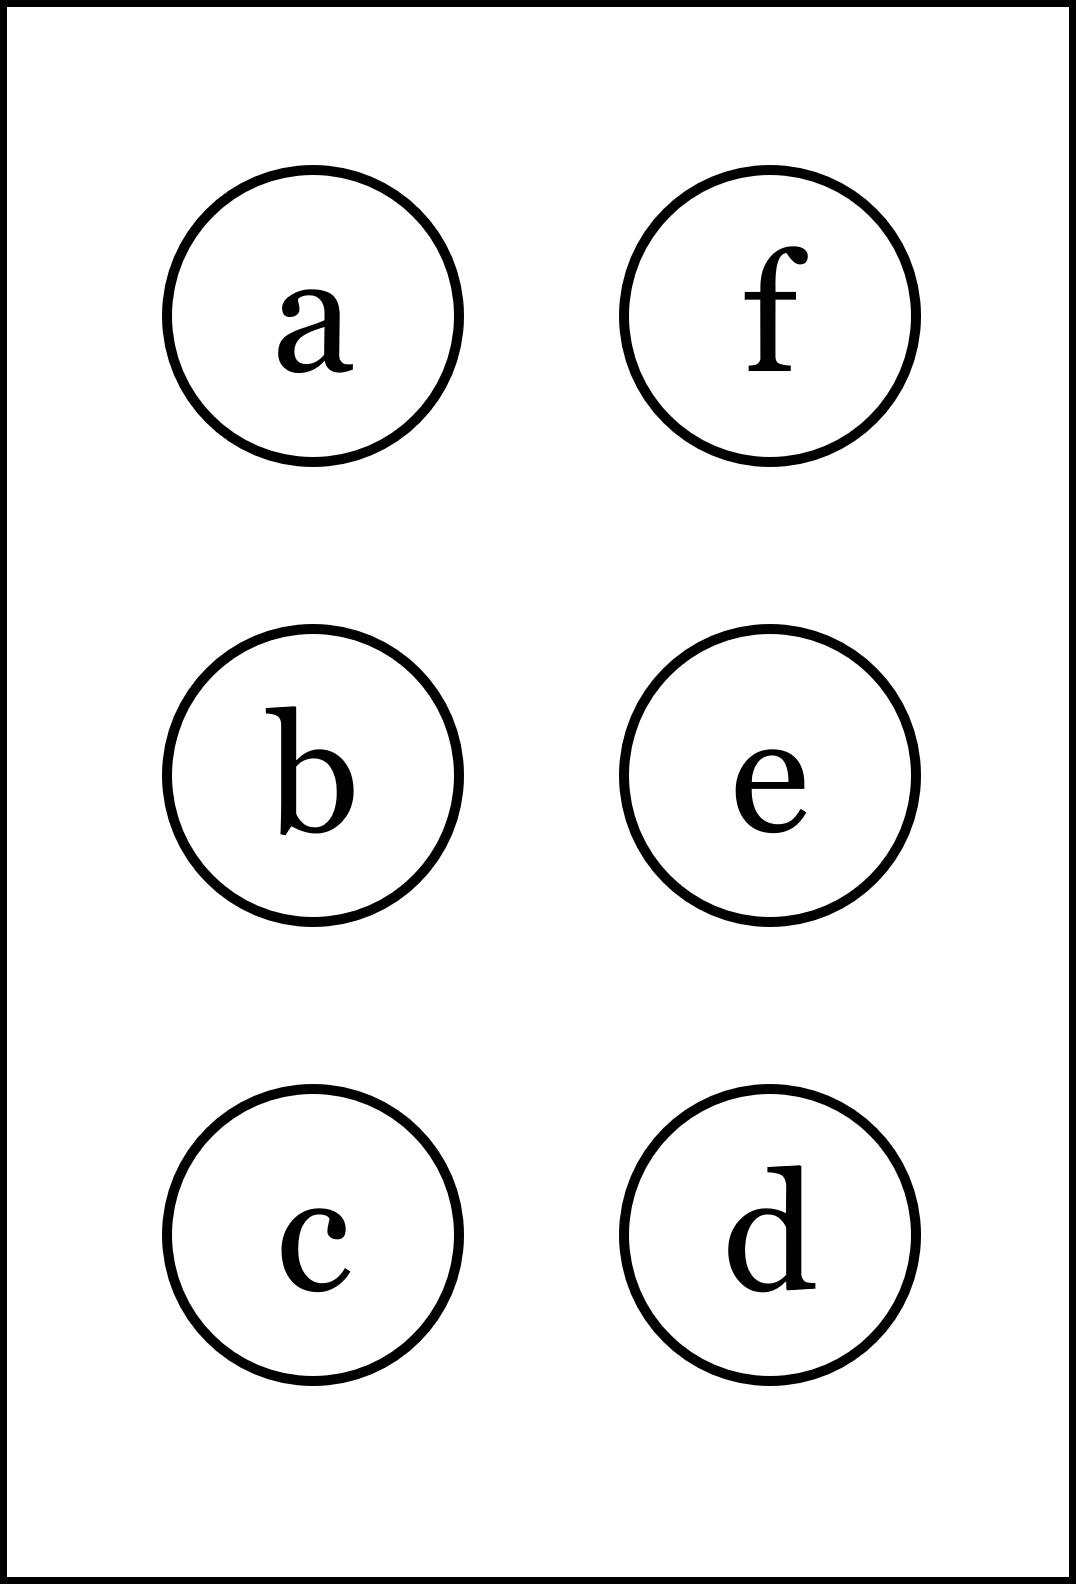
\includegraphics[height=40mm]{../images/braille.png}
{\small Písmeno Braillovej abecedy}
\end{center}
\end{minipage}
\end{center}
\end{minipage}
&
\begin{minipage}[c][104.5mm][t]{0.5\linewidth}
\begin{center}
\vspace{7mm}
{\huge Definiční obor, skupina \textit{Alpha $\alpha$} -\romannumeral2}\\[5mm]
\textit{Jméno:}\phantom{xxxxxxxxxxxxxxxxxxxxxxxxxxxxxxxxxxxxxxxxxxxxxxxxxxxxxxxxxxxxxxxxx}\\[5mm]
\begin{minipage}{0.95\linewidth}
\begin{center}
\textbf{Zjisti definiční obor} zadaných funkcí. Pokud se shoduje s tím za otazníky,\\tak napravo obarvi příslušející kroužek načerno. \textbf{Spolu odevzdejte výsledné slovo}.
\end{center}
\end{minipage}
\\[1mm]
\begin{minipage}{0.79\linewidth}
\begin{center}
\begin{varwidth}{\linewidth}
\begin{enumerate}
\normalsizerrr
\item $f(x)=\cfrac{8x+8}{-7x-2}$\quad \dotfill\; ???\;\dotfill \quad $\mathbb{R}\smallsetminus\{\nicefrac{-2}{7}\}$
\item $f(x)=\cfrac{1}{-2x^3+62x-60}$\quad \dotfill\; ???\;\dotfill \quad $\mathbb{R}\smallsetminus\{1,-6,5\}$
\item $f(x)=5\sqrt{8x+1}$\quad \dotfill\; ???\;\dotfill \quad $x\geq\nicefrac{-1}{8}$
\item $f(x)=\sqrt{-x^2-7x}$\quad \dotfill\; ???\;\dotfill \quad $x\in(-7 , 0)$
\item $f(x)=4\ln{(3x-7)}$\quad \dotfill\; ???\;\dotfill \quad $x>\nicefrac{7}{3}$
\item $f(x)=\ln{(x^2+6x+5)}$\quad \dotfill\; ???\;\dotfill \quad $x\in(-5 , -1)$
\end{enumerate}
\end{varwidth}
\end{center}
\end{minipage}
\begin{minipage}{0.20\linewidth}
\begin{center}
{\Huge\bfseries 2.} \\[2mm]
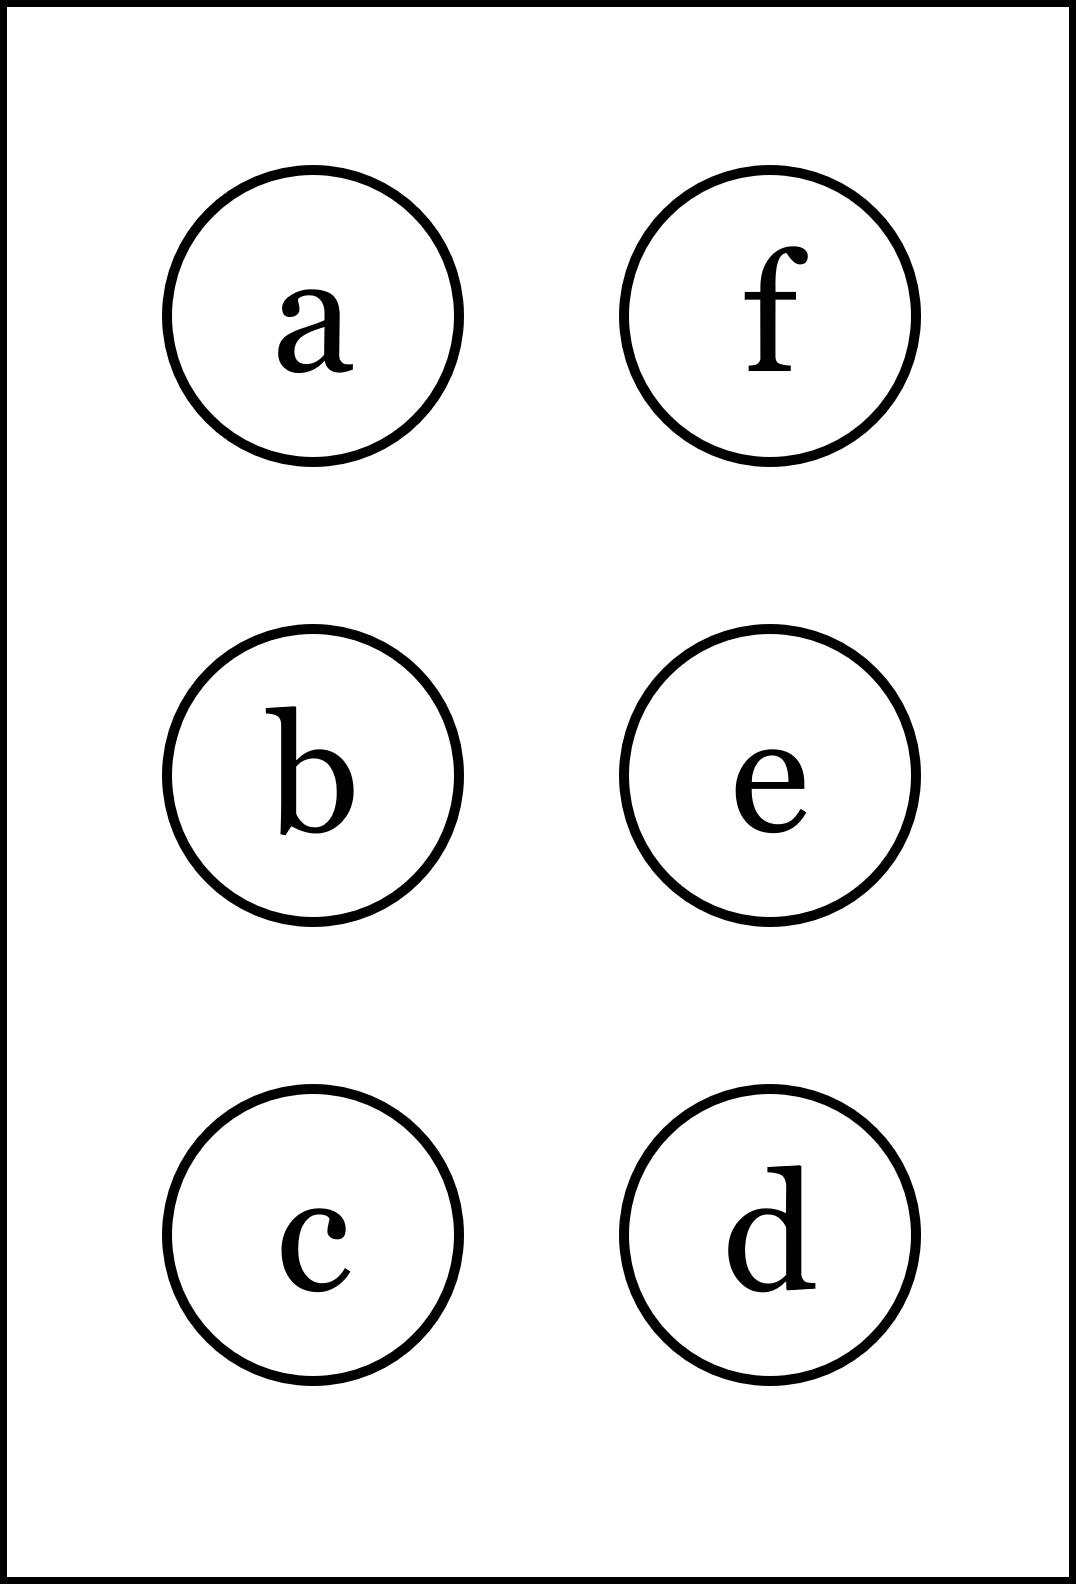
\includegraphics[height=40mm]{../images/braille.png}
{\small Písmeno Braillovej abecedy}
\end{center}
\end{minipage}
\end{center}
\end{minipage}
\\ \hdashline
\begin{minipage}[c][104.5mm][t]{0.5\linewidth}
\begin{center}
\vspace{7mm}
{\huge Definiční obor, skupina \textit{Alpha $\alpha$} -\romannumeral3}\\[5mm]
\textit{Jméno:}\phantom{xxxxxxxxxxxxxxxxxxxxxxxxxxxxxxxxxxxxxxxxxxxxxxxxxxxxxxxxxxxxxxxxx}\\[5mm]
\begin{minipage}{0.95\linewidth}
\begin{center}
\textbf{Zjisti definiční obor} zadaných funkcí. Pokud se shoduje s tím za otazníky,\\tak napravo obarvi příslušející kroužek načerno. \textbf{Spolu odevzdejte výsledné slovo}.
\end{center}
\end{minipage}
\\[1mm]
\begin{minipage}{0.79\linewidth}
\begin{center}
\begin{varwidth}{\linewidth}
\begin{enumerate}
\normalsizerrr
\item $f(x)=\cfrac{-5x+2}{4x+2}$\quad \dotfill\; ???\;\dotfill \quad $\mathbb{R}\smallsetminus\{\nicefrac{-1}{2}\}$
\item $f(x)=\cfrac{1}{x^3-4x^2-28x-32}$\quad \dotfill\; ???\;\dotfill \quad $\mathbb{R}\smallsetminus\{8,2,-1\}$
\item $f(x)=-2\sqrt{-3x+2}$\quad \dotfill\; ???\;\dotfill \quad $x\geq\nicefrac{2}{3}$
\item $f(x)=\sqrt{-x^2+4x}$\quad \dotfill\; ???\;\dotfill \quad $x\in\langle0 , 4\rangle$
\item $f(x)=3\ln{(-x+7)}$\quad \dotfill\; ???\;\dotfill \quad $x>7$
\item $f(x)=\ln{(x^2+7x-8)}$\quad \dotfill\; ???\;\dotfill \quad $x\in(-8 , 1)$
\end{enumerate}
\end{varwidth}
\end{center}
\end{minipage}
\begin{minipage}{0.20\linewidth}
\begin{center}
{\Huge\bfseries 3.} \\[2mm]
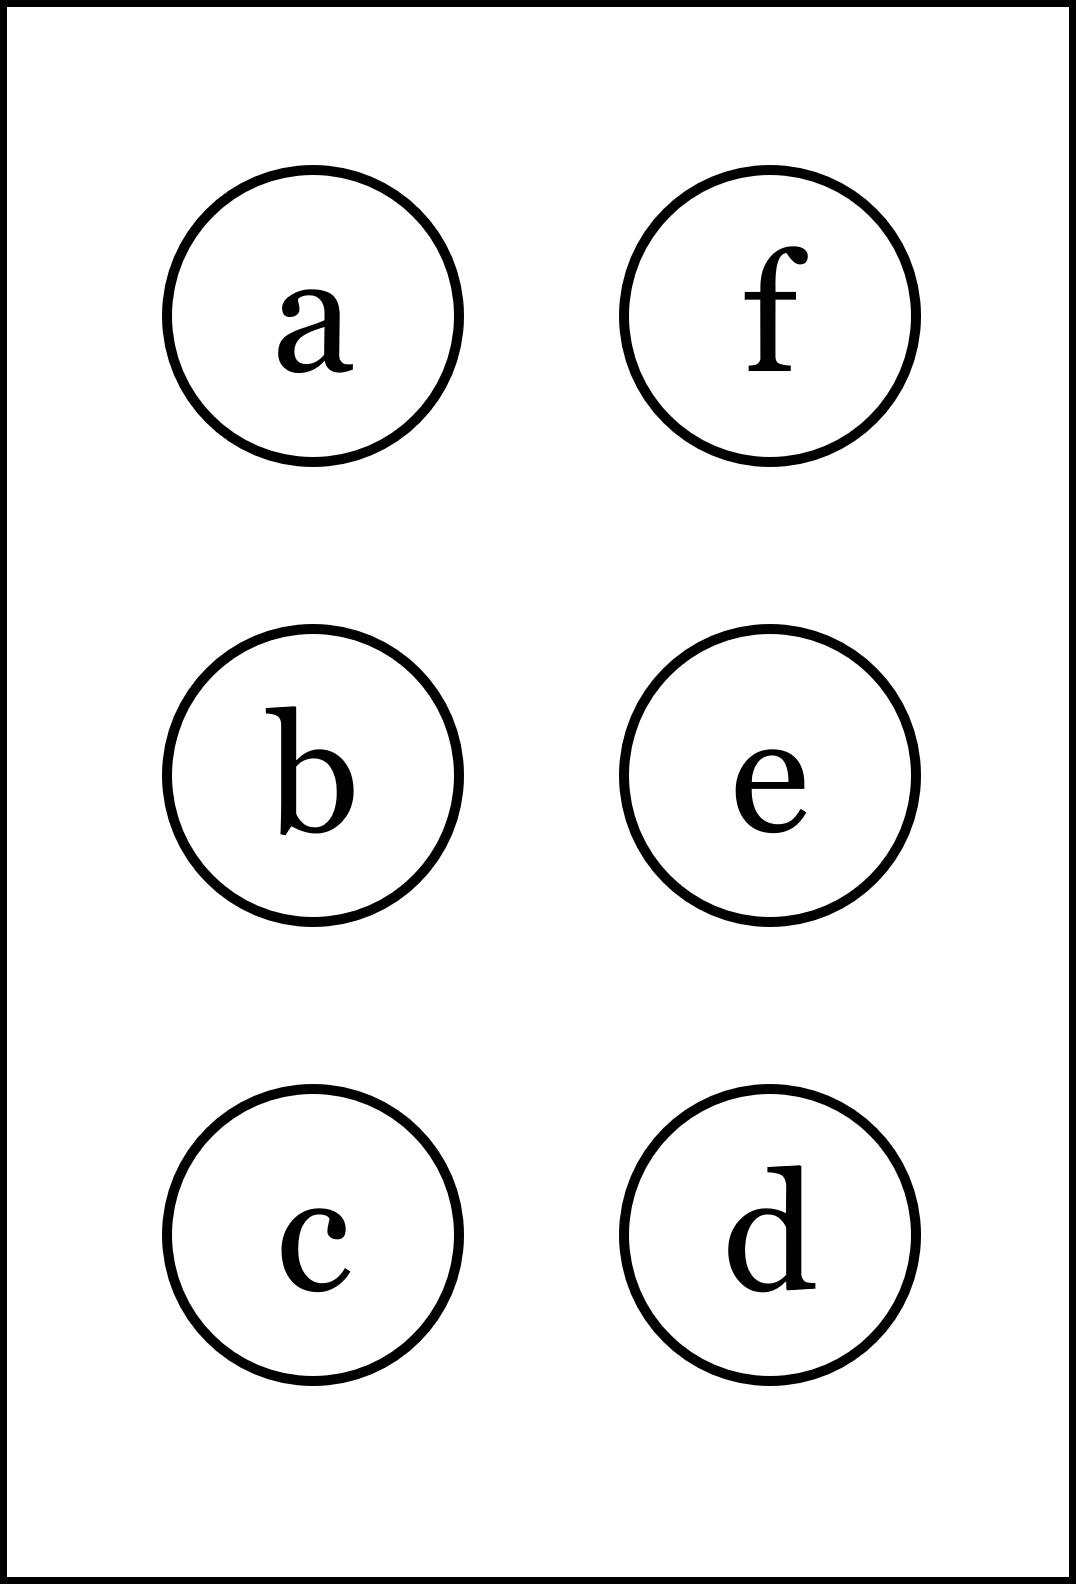
\includegraphics[height=40mm]{../images/braille.png}
{\small Písmeno Braillovej abecedy}
\end{center}
\end{minipage}
\end{center}
\end{minipage}
&
\begin{minipage}[c][104.5mm][t]{0.5\linewidth}
\begin{center}
\vspace{7mm}
{\huge Definiční obor, skupina \textit{Alpha $\alpha$} -\romannumeral4}\\[5mm]
\textit{Jméno:}\phantom{xxxxxxxxxxxxxxxxxxxxxxxxxxxxxxxxxxxxxxxxxxxxxxxxxxxxxxxxxxxxxxxxx}\\[5mm]
\begin{minipage}{0.95\linewidth}
\begin{center}
\textbf{Zjisti definiční obor} zadaných funkcí. Pokud se shoduje s tím za otazníky,\\tak napravo obarvi příslušející kroužek načerno. \textbf{Spolu odevzdejte výsledné slovo}.
\end{center}
\end{minipage}
\\[1mm]
\begin{minipage}{0.79\linewidth}
\begin{center}
\begin{varwidth}{\linewidth}
\begin{enumerate}
\normalsizerrr
\item $f(x)=\cfrac{3x+8}{-x+1}$\quad \dotfill\; ???\;\dotfill \quad $\mathbb{R}\smallsetminus\{-1\}$
\item $f(x)=\cfrac{1}{2x^3-4x^2-2x+4}$\quad \dotfill\; ???\;\dotfill \quad $\mathbb{R}\smallsetminus\{1,2,-1\}$
\item $f(x)=8\sqrt{2x+8}$\quad \dotfill\; ???\;\dotfill \quad $x\geq-4$
\item $f(x)=\sqrt{-x^2-2x}$\quad \dotfill\; ???\;\dotfill \quad $x\in\langle0 , 2\rangle$
\item $f(x)=-5\ln{(5x-3)}$\quad \dotfill\; ???\;\dotfill \quad $x>\nicefrac{3}{5}$
\item $f(x)=\ln{(x^2-4)}$\quad \dotfill\; ???\;\dotfill \quad $x\in(-\infty , -2)\cup(2 , \infty)$
\end{enumerate}
\end{varwidth}
\end{center}
\end{minipage}
\begin{minipage}{0.20\linewidth}
\begin{center}
{\Huge\bfseries 4.} \\[2mm]
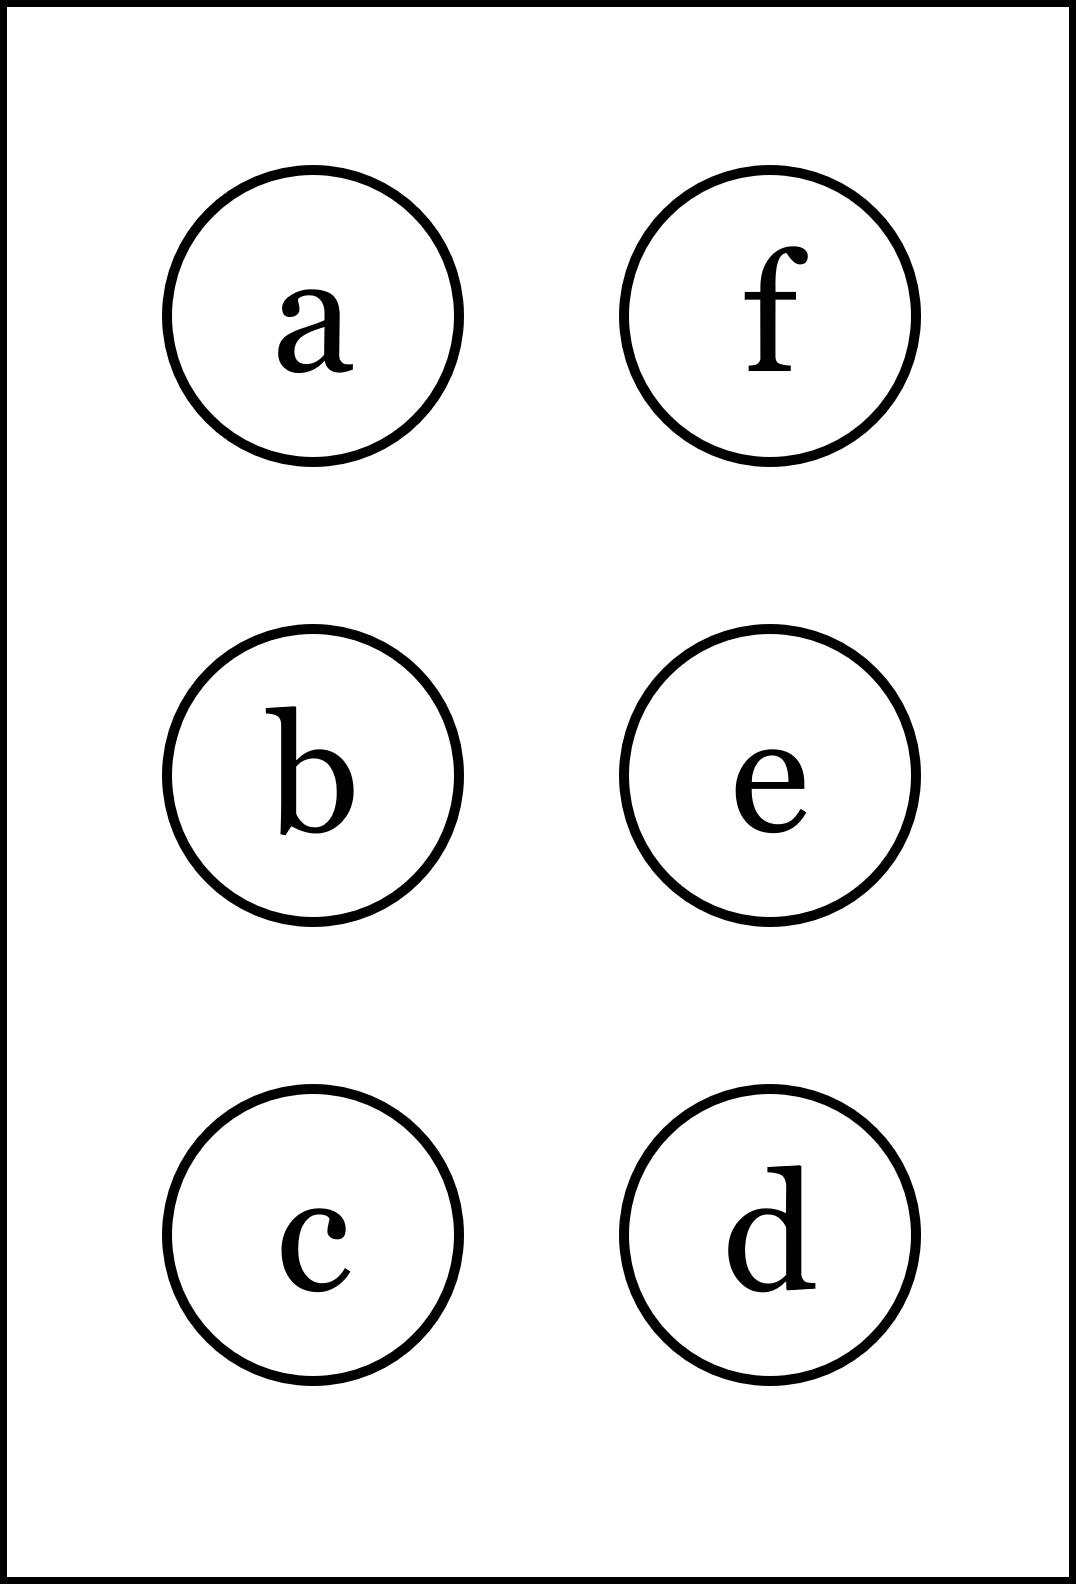
\includegraphics[height=40mm]{../images/braille.png}
{\small Písmeno Braillovej abecedy}
\end{center}
\end{minipage}
\end{center}
\end{minipage}
%
\end{tabular}
\newpage
\thispagestyle{empty}
\begin{tabular}{c:c}
\begin{minipage}[c][104.5mm][t]{0.5\linewidth}
\begin{center}
\vspace{7mm}
{\huge Definiční obor, skupina \textit{Beta $\beta$} -\romannumeral1}\\[5mm]
\textit{Jméno:}\phantom{xxxxxxxxxxxxxxxxxxxxxxxxxxxxxxxxxxxxxxxxxxxxxxxxxxxxxxxxxxxxxxxxx}\\[5mm]
\begin{minipage}{0.95\linewidth}
\begin{center}
\textbf{Zjisti definiční obor} zadaných funkcí. Pokud se shoduje s tím za otazníky,\\tak napravo obarvi příslušející kroužek načerno. \textbf{Spolu odevzdejte výsledné slovo}.
\end{center}
\end{minipage}
\\[1mm]
\begin{minipage}{0.79\linewidth}
\begin{center}
\begin{varwidth}{\linewidth}
\begin{enumerate}
\normalsizerrr
\item $f(x)=\cfrac{3x+5}{x-1}$\quad \dotfill\; ???\;\dotfill \quad $\mathbb{R}\smallsetminus\{1\}$
\item $f(x)=\cfrac{1}{-4x^3-4x^2+16x+16}$\quad \dotfill\; ???\;\dotfill \quad $\mathbb{R}\smallsetminus\{-2\}$
\item $f(x)=-3\sqrt{4x-3}$\quad \dotfill\; ???\;\dotfill \quad $x\geq\nicefrac{3}{4}$
\item $f(x)=\sqrt{-x^2-6x}$\quad \dotfill\; ???\;\dotfill \quad $x\in\langle-6 , 0\rangle$
\item $f(x)=3\ln{(6x-1)}$\quad \dotfill\; ???\;\dotfill \quad $x>\nicefrac{1}{6}$
\item $f(x)=\ln{(x^2-5x+6)}$\quad \dotfill\; ???\;\dotfill \quad $x\in(2 , 3)$
\end{enumerate}
\end{varwidth}
\end{center}
\end{minipage}
\begin{minipage}{0.20\linewidth}
\begin{center}
{\Huge\bfseries 1.} \\[2mm]
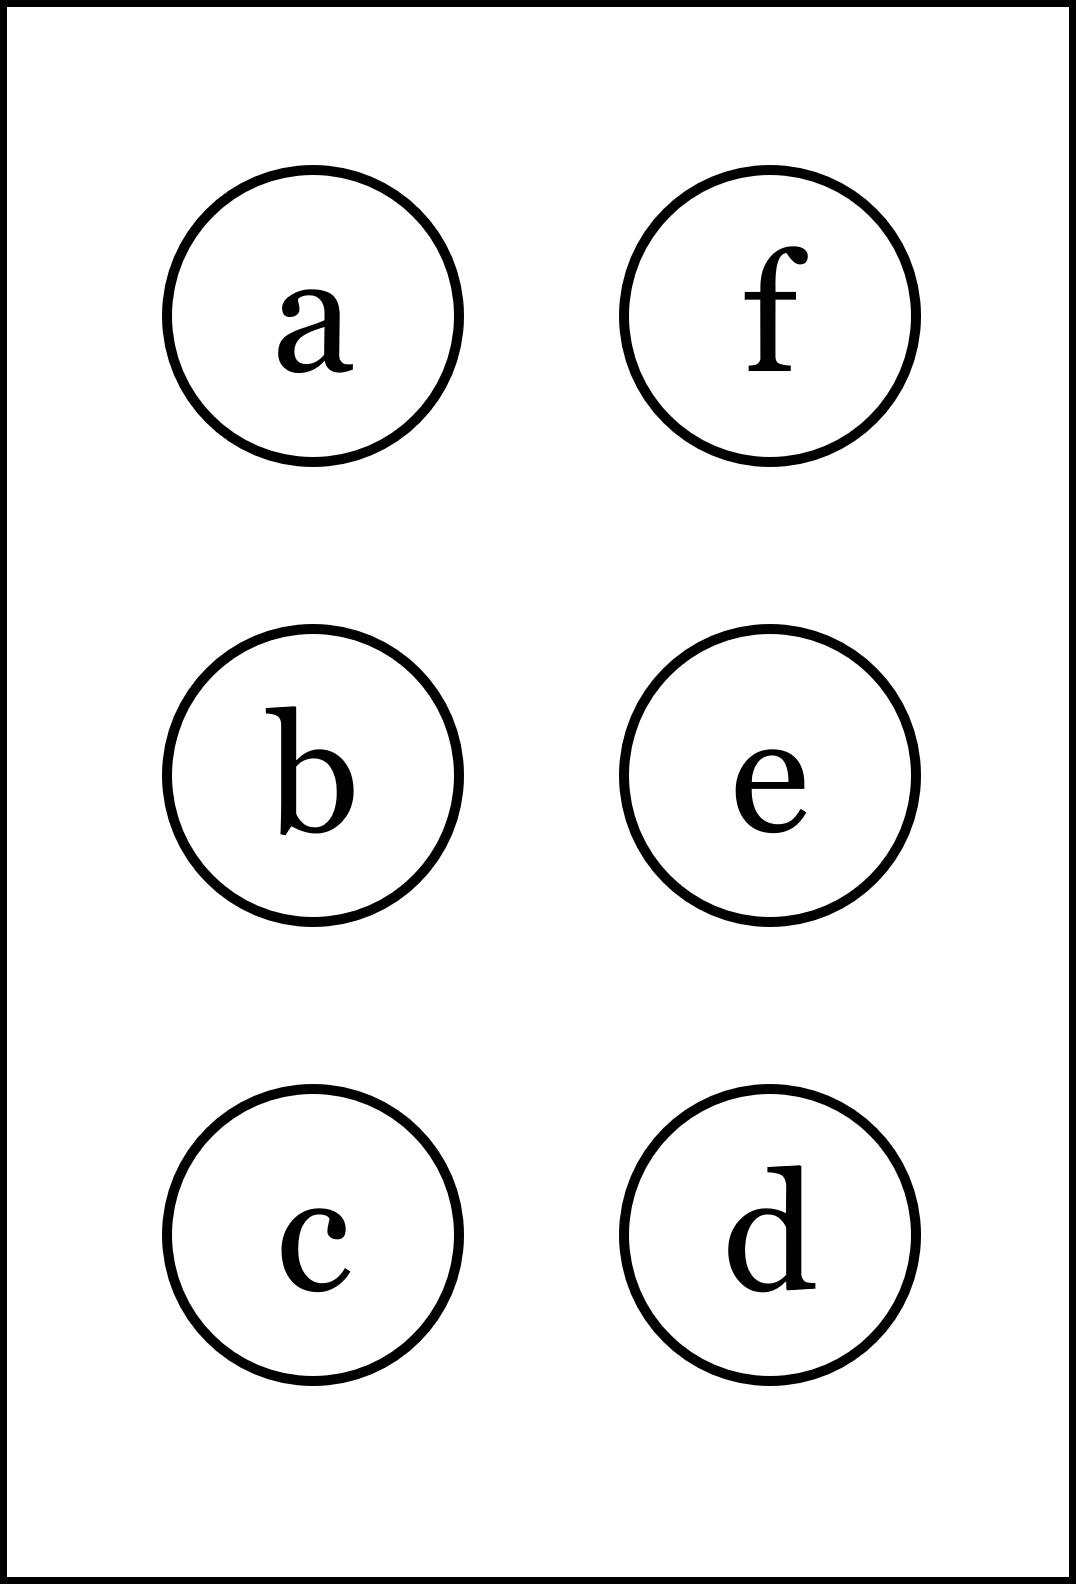
\includegraphics[height=40mm]{../images/braille.png}
{\small Písmeno Braillovej abecedy}
\end{center}
\end{minipage}
\end{center}
\end{minipage}
&
\begin{minipage}[c][104.5mm][t]{0.5\linewidth}
\begin{center}
\vspace{7mm}
{\huge Definiční obor, skupina \textit{Beta $\beta$} -\romannumeral2}\\[5mm]
\textit{Jméno:}\phantom{xxxxxxxxxxxxxxxxxxxxxxxxxxxxxxxxxxxxxxxxxxxxxxxxxxxxxxxxxxxxxxxxx}\\[5mm]
\begin{minipage}{0.95\linewidth}
\begin{center}
\textbf{Zjisti definiční obor} zadaných funkcí. Pokud se shoduje s tím za otazníky,\\tak napravo obarvi příslušející kroužek načerno. \textbf{Spolu odevzdejte výsledné slovo}.
\end{center}
\end{minipage}
\\[1mm]
\begin{minipage}{0.79\linewidth}
\begin{center}
\begin{varwidth}{\linewidth}
\begin{enumerate}
\normalsizerrr
\item $f(x)=\cfrac{-5x+5}{-2x+4}$\quad \dotfill\; ???\;\dotfill \quad $\mathbb{R}\smallsetminus\{-2\}$
\item $f(x)=\cfrac{1}{3x^3+18x^2-45x+24}$\quad \dotfill\; ???\;\dotfill \quad $\mathbb{R}\smallsetminus\{-8,1\}$
\item $f(x)=3\sqrt{2x-1}$\quad \dotfill\; ???\;\dotfill \quad $x\leq\nicefrac{1}{2}$
\item $f(x)=\sqrt{-x^2+2x}$\quad \dotfill\; ???\;\dotfill \quad $x\in\langle-2 , 0\rangle$
\item $f(x)=-7\ln{(-7x-5)}$\quad \dotfill\; ???\;\dotfill \quad $x>\nicefrac{-5}{7}$
\item $f(x)=\ln{(x^2-2x-48)}$\quad \dotfill\; ???\;\dotfill \quad $x\in(-\infty , -6)\cup(8 , \infty)$
\end{enumerate}
\end{varwidth}
\end{center}
\end{minipage}
\begin{minipage}{0.20\linewidth}
\begin{center}
{\Huge\bfseries 2.} \\[2mm]
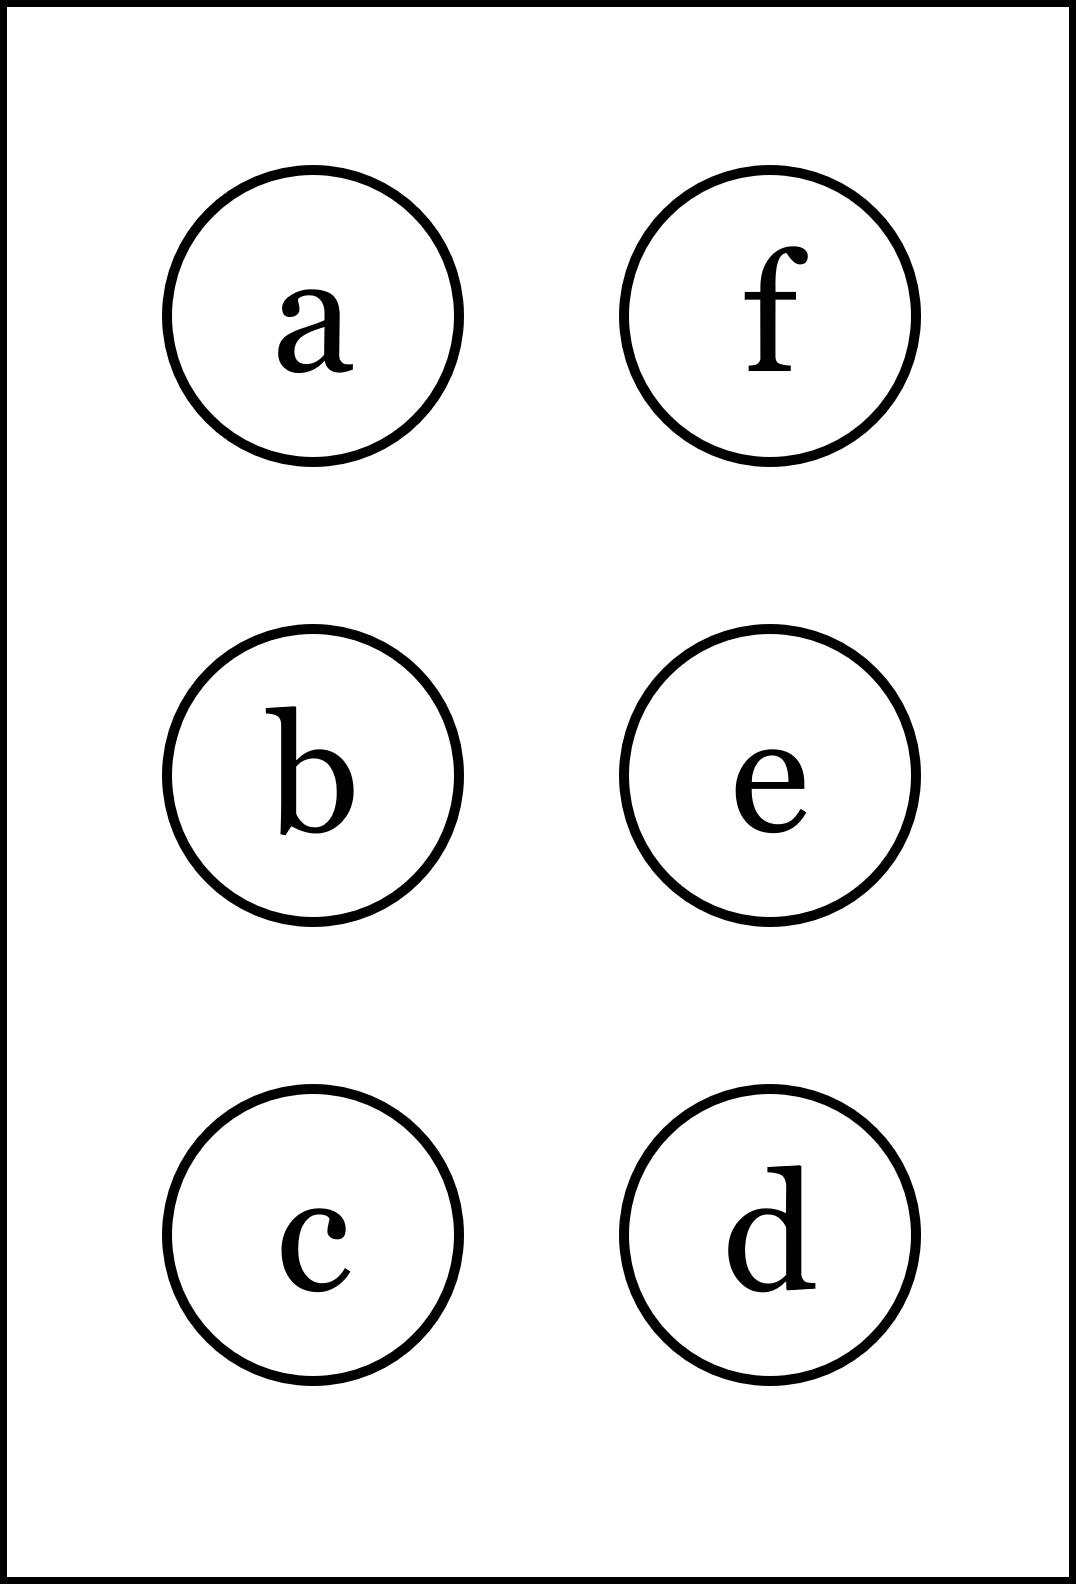
\includegraphics[height=40mm]{../images/braille.png}
{\small Písmeno Braillovej abecedy}
\end{center}
\end{minipage}
\end{center}
\end{minipage}
\\ \hdashline
\begin{minipage}[c][104.5mm][t]{0.5\linewidth}
\begin{center}
\vspace{7mm}
{\huge Definiční obor, skupina \textit{Beta $\beta$} -\romannumeral3}\\[5mm]
\textit{Jméno:}\phantom{xxxxxxxxxxxxxxxxxxxxxxxxxxxxxxxxxxxxxxxxxxxxxxxxxxxxxxxxxxxxxxxxx}\\[5mm]
\begin{minipage}{0.95\linewidth}
\begin{center}
\textbf{Zjisti definiční obor} zadaných funkcí. Pokud se shoduje s tím za otazníky,\\tak napravo obarvi příslušející kroužek načerno. \textbf{Spolu odevzdejte výsledné slovo}.
\end{center}
\end{minipage}
\\[1mm]
\begin{minipage}{0.79\linewidth}
\begin{center}
\begin{varwidth}{\linewidth}
\begin{enumerate}
\normalsizerrr
\item $f(x)=\cfrac{-x-1}{2x-5}$\quad \dotfill\; ???\;\dotfill \quad $\mathbb{R}\smallsetminus\{\nicefrac{5}{2}\}$
\item $f(x)=\cfrac{1}{2x^3-12x^2+6x+20}$\quad \dotfill\; ???\;\dotfill \quad $\mathbb{R}\smallsetminus\{1,2,4\}$
\item $f(x)=-\sqrt{x-2}$\quad \dotfill\; ???\;\dotfill \quad $x\geq2$
\item $f(x)=\sqrt{-x^2+8x}$\quad \dotfill\; ???\;\dotfill \quad $x\in(0 , 8)$
\item $f(x)=4\ln{(2x-2)}$\quad \dotfill\; ???\;\dotfill \quad $x>-1$
\item $f(x)=\ln{(x^2+2x-8)}$\quad \dotfill\; ???\;\dotfill \quad $x\in(-\infty , -4)\cup(2 , \infty)$
\end{enumerate}
\end{varwidth}
\end{center}
\end{minipage}
\begin{minipage}{0.20\linewidth}
\begin{center}
{\Huge\bfseries 3.} \\[2mm]
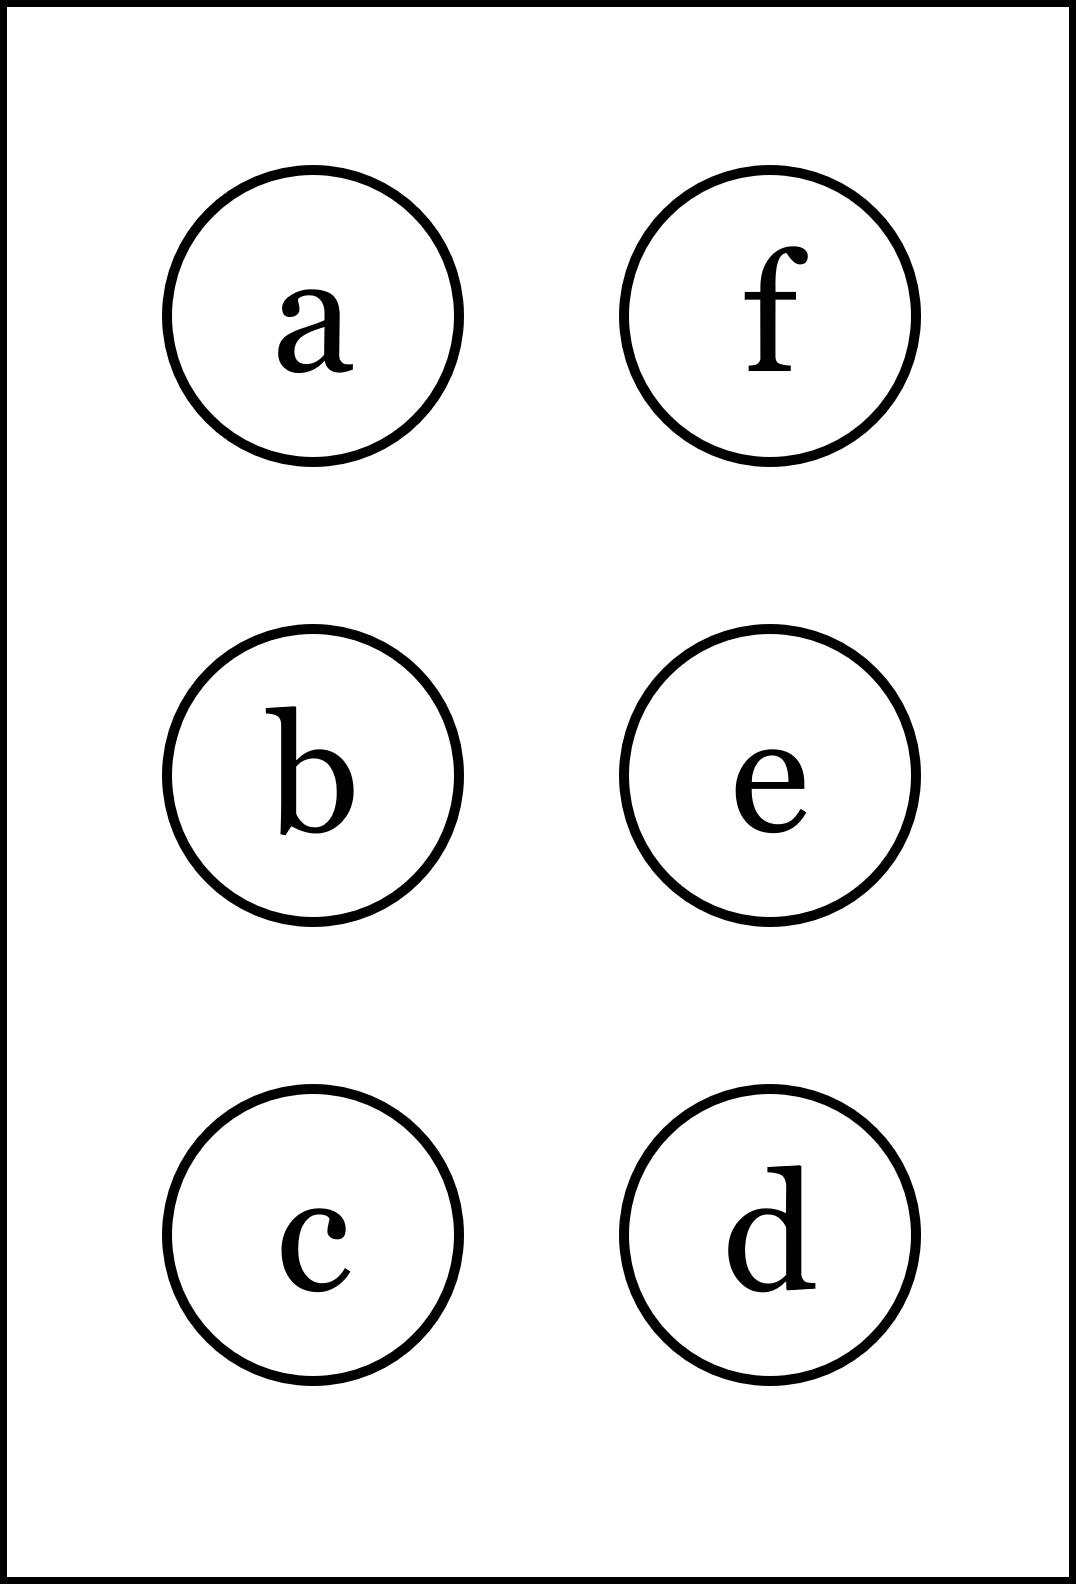
\includegraphics[height=40mm]{../images/braille.png}
{\small Písmeno Braillovej abecedy}
\end{center}
\end{minipage}
\end{center}
\end{minipage}
&
\begin{minipage}[c][104.5mm][t]{0.5\linewidth}
\begin{center}
\vspace{7mm}
{\huge Definiční obor, skupina \textit{Beta $\beta$} -\romannumeral4}\\[5mm]
\textit{Jméno:}\phantom{xxxxxxxxxxxxxxxxxxxxxxxxxxxxxxxxxxxxxxxxxxxxxxxxxxxxxxxxxxxxxxxxx}\\[5mm]
\begin{minipage}{0.95\linewidth}
\begin{center}
\textbf{Zjisti definiční obor} zadaných funkcí. Pokud se shoduje s tím za otazníky,\\tak napravo obarvi příslušející kroužek načerno. \textbf{Spolu odevzdejte výsledné slovo}.
\end{center}
\end{minipage}
\\[1mm]
\begin{minipage}{0.79\linewidth}
\begin{center}
\begin{varwidth}{\linewidth}
\begin{enumerate}
\normalsizerrr
\item $f(x)=\cfrac{-2x+5}{4x-1}$\quad \dotfill\; ???\;\dotfill \quad $\mathbb{R}\smallsetminus\{\nicefrac{1}{4}\}$
\item $f(x)=\cfrac{1}{x^3-5x^2-22x+56}$\quad \dotfill\; ???\;\dotfill \quad $\mathbb{R}\smallsetminus\{8,-4,-2\}$
\item $f(x)=-6\sqrt{-3x-3}$\quad \dotfill\; ???\;\dotfill \quad $x\leq1$
\item $f(x)=\sqrt{-x^2+7x}$\quad \dotfill\; ???\;\dotfill \quad $x\in\langle-7 , 0\rangle$
\item $f(x)=-\ln{(-4x-4)}$\quad \dotfill\; ???\;\dotfill \quad $x<1$
\item $f(x)=\ln{(x^2-10x+21)}$\quad \dotfill\; ???\;\dotfill \quad $x\in(3 , 7)$
\end{enumerate}
\end{varwidth}
\end{center}
\end{minipage}
\begin{minipage}{0.20\linewidth}
\begin{center}
{\Huge\bfseries 4.} \\[2mm]
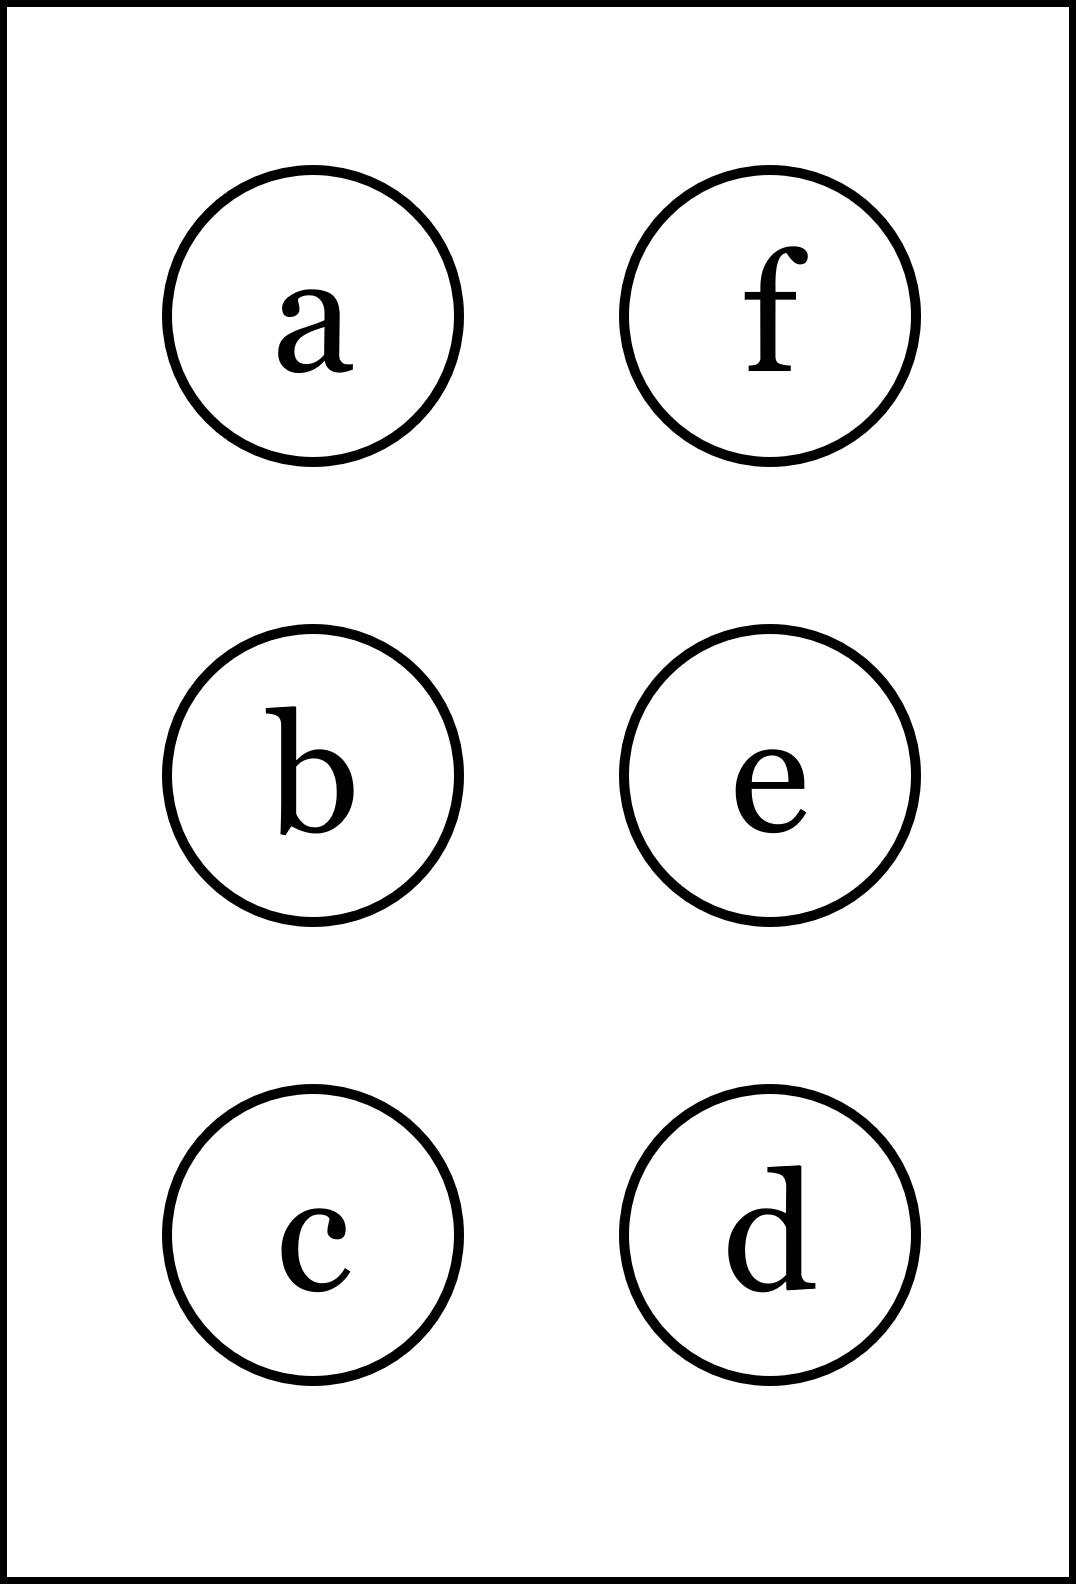
\includegraphics[height=40mm]{../images/braille.png}
{\small Písmeno Braillovej abecedy}
\end{center}
\end{minipage}
\end{center}
\end{minipage}
%
\end{tabular}
\newpage
\thispagestyle{empty}
\begin{tabular}{c:c}
\begin{minipage}[c][104.5mm][t]{0.5\linewidth}
\begin{center}
\vspace{7mm}
{\huge Definiční obor, skupina \textit{Gamma $\gamma$} -\romannumeral1}\\[5mm]
\textit{Jméno:}\phantom{xxxxxxxxxxxxxxxxxxxxxxxxxxxxxxxxxxxxxxxxxxxxxxxxxxxxxxxxxxxxxxxxx}\\[5mm]
\begin{minipage}{0.95\linewidth}
\begin{center}
\textbf{Zjisti definiční obor} zadaných funkcí. Pokud se shoduje s tím za otazníky,\\tak napravo obarvi příslušející kroužek načerno. \textbf{Spolu odevzdejte výsledné slovo}.
\end{center}
\end{minipage}
\\[1mm]
\begin{minipage}{0.79\linewidth}
\begin{center}
\begin{varwidth}{\linewidth}
\begin{enumerate}
\normalsizerrr
\item $f(x)=\cfrac{4x-6}{x-2}$\quad \dotfill\; ???\;\dotfill \quad $\mathbb{R}\smallsetminus\{2\}$
\item $f(x)=\cfrac{1}{-x^3+11x^2-34x+24}$\quad \dotfill\; ???\;\dotfill \quad $\mathbb{R}\smallsetminus\{1,4,-4\}$
\item $f(x)=\sqrt{2x+2}$\quad \dotfill\; ???\;\dotfill \quad $x\leq-1$
\item $f(x)=\sqrt{-x^2-6x}$\quad \dotfill\; ???\;\dotfill \quad $x\in(-6 , 0)$
\item $f(x)=-4\ln{(-2x-5)}$\quad \dotfill\; ???\;\dotfill \quad $x<\nicefrac{-5}{2}$
\item $f(x)=\ln{(x^2+11x+24)}$\quad \dotfill\; ???\;\dotfill \quad $x\in(-8 , -3)$
\end{enumerate}
\end{varwidth}
\end{center}
\end{minipage}
\begin{minipage}{0.20\linewidth}
\begin{center}
{\Huge\bfseries 1.} \\[2mm]
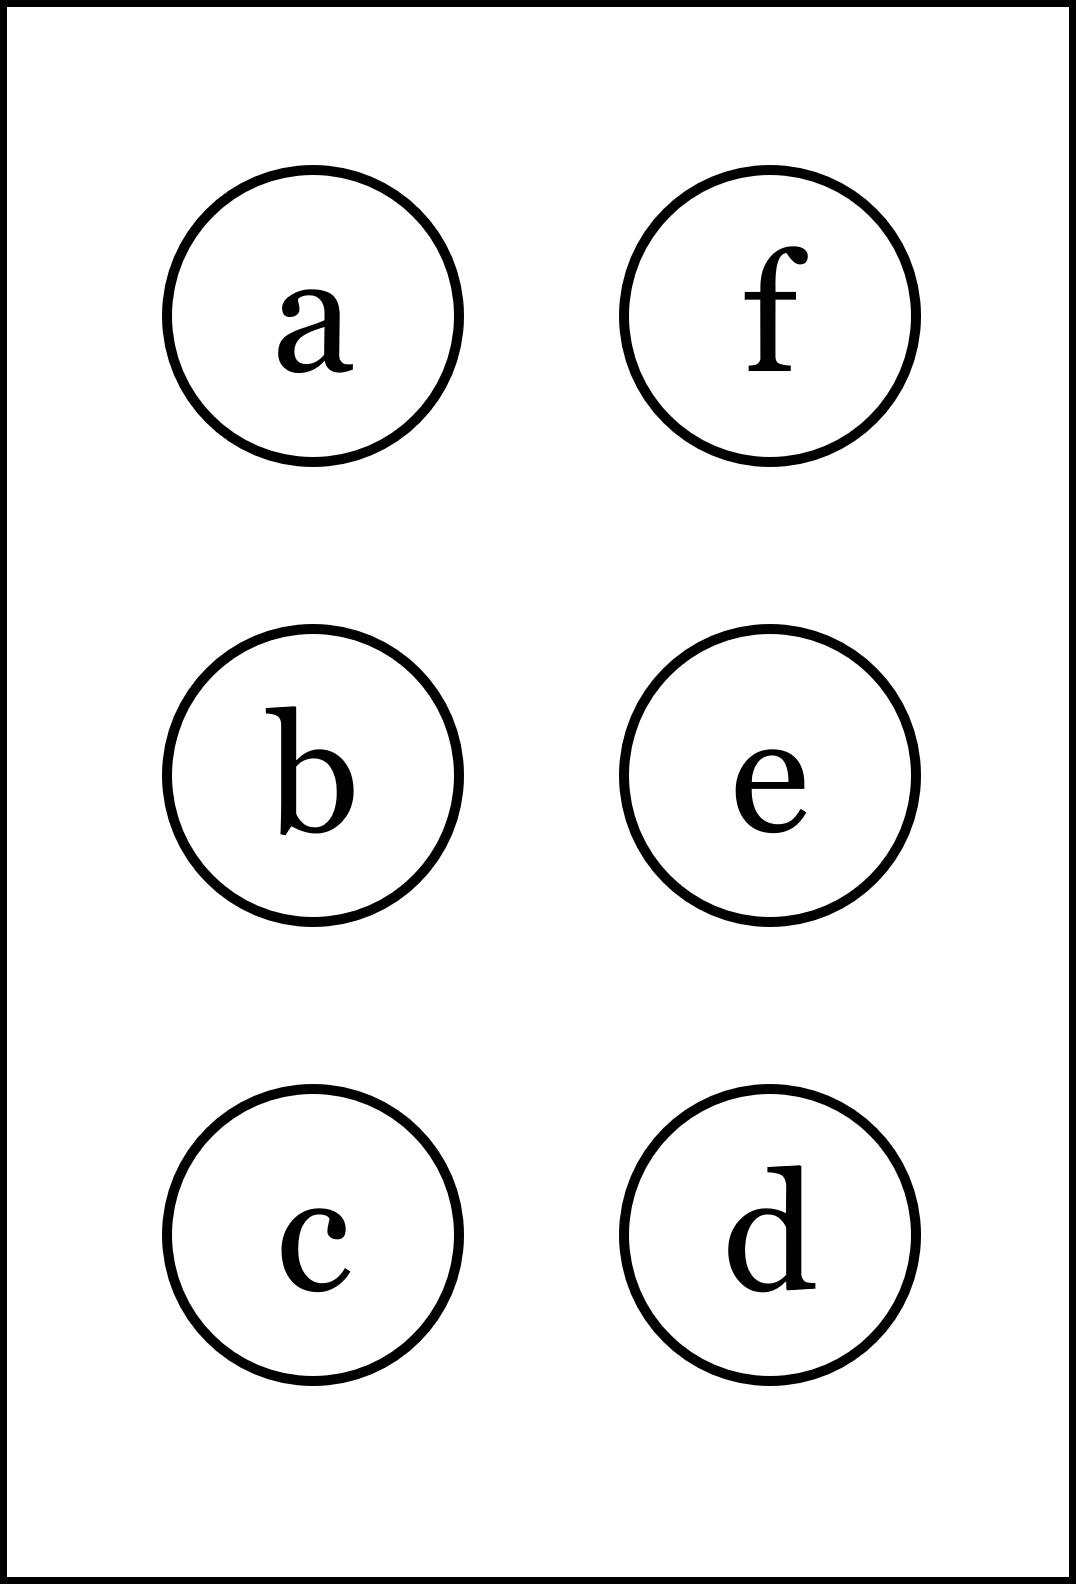
\includegraphics[height=40mm]{../images/braille.png}
{\small Písmeno Braillovej abecedy}
\end{center}
\end{minipage}
\end{center}
\end{minipage}
&
\begin{minipage}[c][104.5mm][t]{0.5\linewidth}
\begin{center}
\vspace{7mm}
{\huge Definiční obor, skupina \textit{Gamma $\gamma$} -\romannumeral2}\\[5mm]
\textit{Jméno:}\phantom{xxxxxxxxxxxxxxxxxxxxxxxxxxxxxxxxxxxxxxxxxxxxxxxxxxxxxxxxxxxxxxxxx}\\[5mm]
\begin{minipage}{0.95\linewidth}
\begin{center}
\textbf{Zjisti definiční obor} zadaných funkcí. Pokud se shoduje s tím za otazníky,\\tak napravo obarvi příslušející kroužek načerno. \textbf{Spolu odevzdejte výsledné slovo}.
\end{center}
\end{minipage}
\\[1mm]
\begin{minipage}{0.79\linewidth}
\begin{center}
\begin{varwidth}{\linewidth}
\begin{enumerate}
\normalsizerrr
\item $f(x)=\cfrac{5x+2}{2x-1}$\quad \dotfill\; ???\;\dotfill \quad $\mathbb{R}\smallsetminus\{\nicefrac{1}{2}\}$
\item $f(x)=\cfrac{1}{2x^3-8x^2-30x+36}$\quad \dotfill\; ???\;\dotfill \quad $\mathbb{R}\smallsetminus\{-5,6,-1\}$
\item $f(x)=9\sqrt{4x-6}$\quad \dotfill\; ???\;\dotfill \quad $x\geq\nicefrac{3}{2}$
\item $f(x)=\sqrt{-x^2+6x}$\quad \dotfill\; ???\;\dotfill \quad $x\in\langle-6 , 0\rangle$
\item $f(x)=-\ln{(-2x+5)}$\quad \dotfill\; ???\;\dotfill \quad $x<\nicefrac{-5}{2}$
\item $f(x)=\ln{(x^2-6x+8)}$\quad \dotfill\; ???\;\dotfill \quad $x\in(-\infty , 2)\cup(4 , \infty)$
\end{enumerate}
\end{varwidth}
\end{center}
\end{minipage}
\begin{minipage}{0.20\linewidth}
\begin{center}
{\Huge\bfseries 2.} \\[2mm]
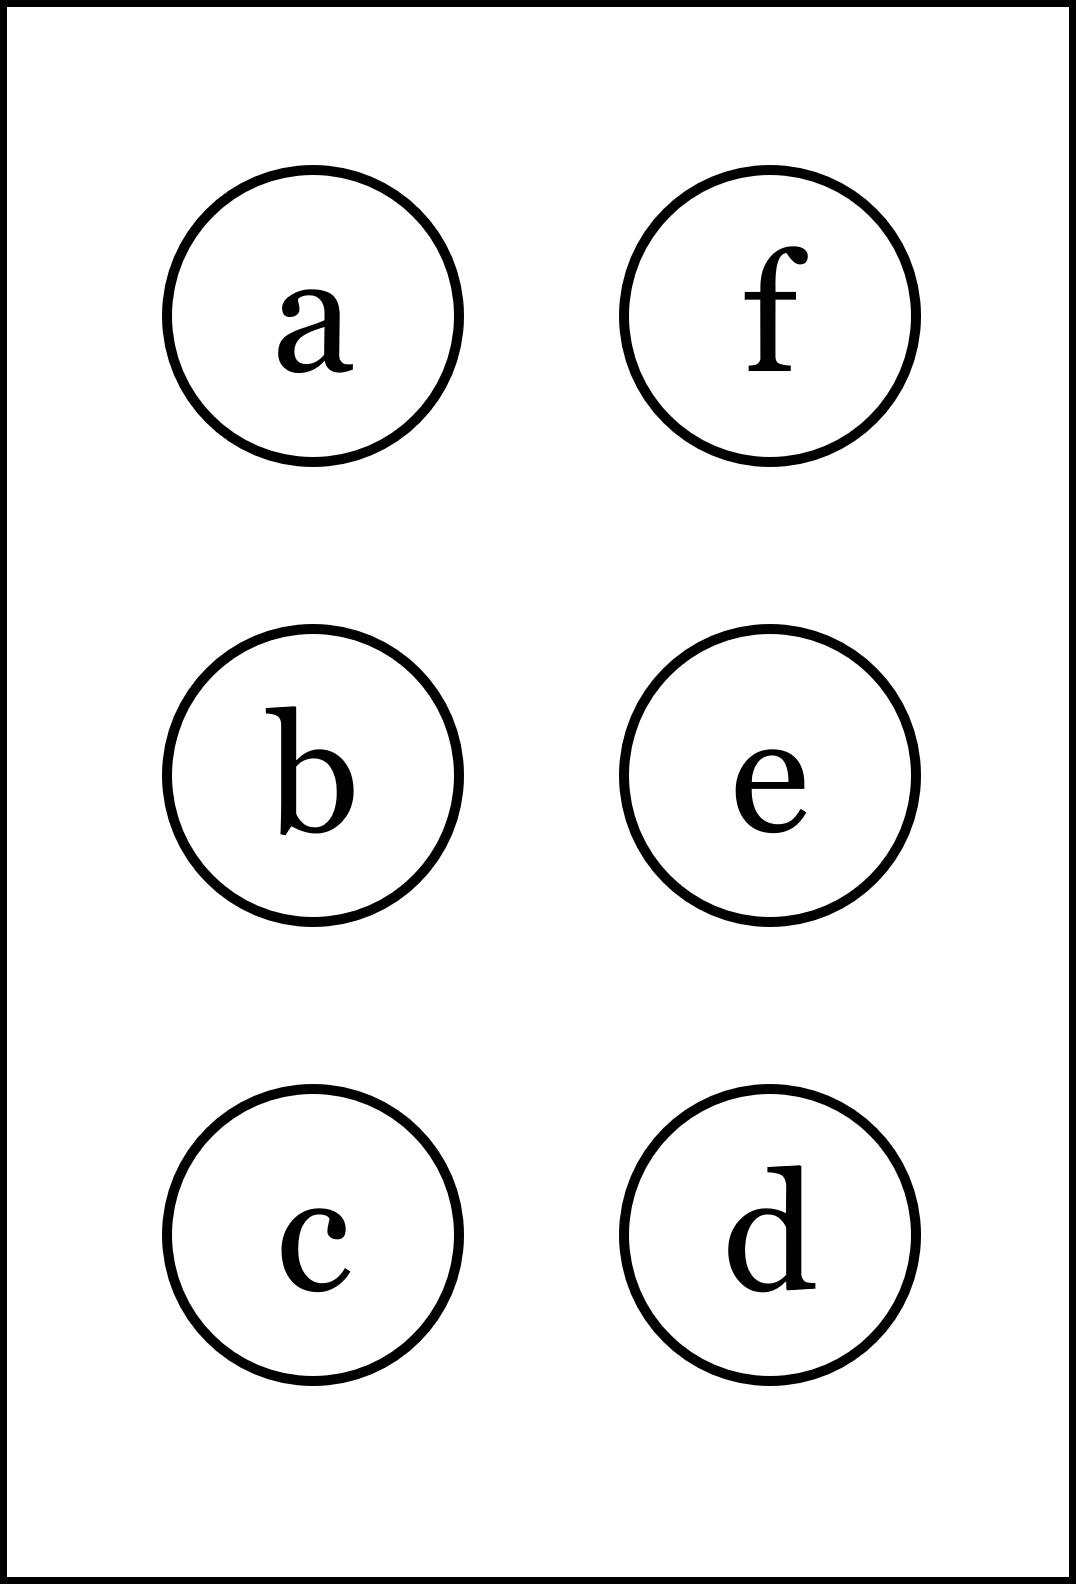
\includegraphics[height=40mm]{../images/braille.png}
{\small Písmeno Braillovej abecedy}
\end{center}
\end{minipage}
\end{center}
\end{minipage}
\\ \hdashline
\begin{minipage}[c][104.5mm][t]{0.5\linewidth}
\begin{center}
\vspace{7mm}
{\huge Definiční obor, skupina \textit{Gamma $\gamma$} -\romannumeral3}\\[5mm]
\textit{Jméno:}\phantom{xxxxxxxxxxxxxxxxxxxxxxxxxxxxxxxxxxxxxxxxxxxxxxxxxxxxxxxxxxxxxxxxx}\\[5mm]
\begin{minipage}{0.95\linewidth}
\begin{center}
\textbf{Zjisti definiční obor} zadaných funkcí. Pokud se shoduje s tím za otazníky,\\tak napravo obarvi příslušející kroužek načerno. \textbf{Spolu odevzdejte výsledné slovo}.
\end{center}
\end{minipage}
\\[1mm]
\begin{minipage}{0.79\linewidth}
\begin{center}
\begin{varwidth}{\linewidth}
\begin{enumerate}
\normalsizerrr
\item $f(x)=\cfrac{6x-1}{-3x+1}$\quad \dotfill\; ???\;\dotfill \quad $\mathbb{R}\smallsetminus\{\nicefrac{-1}{3}\}$
\item $f(x)=\cfrac{1}{-x^3-9x^2-27x-27}$\quad \dotfill\; ???\;\dotfill \quad $\mathbb{R}\smallsetminus\{-3\}$
\item $f(x)=4\sqrt{-3x-2}$\quad \dotfill\; ???\;\dotfill \quad $x\leq\nicefrac{2}{3}$
\item $f(x)=\sqrt{-x^2-9x}$\quad \dotfill\; ???\;\dotfill \quad $x\in(-9 , 0)$
\item $f(x)=-3\ln{(5x-3)}$\quad \dotfill\; ???\;\dotfill \quad $x<\nicefrac{3}{5}$
\item $f(x)=\ln{(x^2+2x-15)}$\quad \dotfill\; ???\;\dotfill \quad $x\in(-\infty , -5)\cup(3 , \infty)$
\end{enumerate}
\end{varwidth}
\end{center}
\end{minipage}
\begin{minipage}{0.20\linewidth}
\begin{center}
{\Huge\bfseries 3.} \\[2mm]
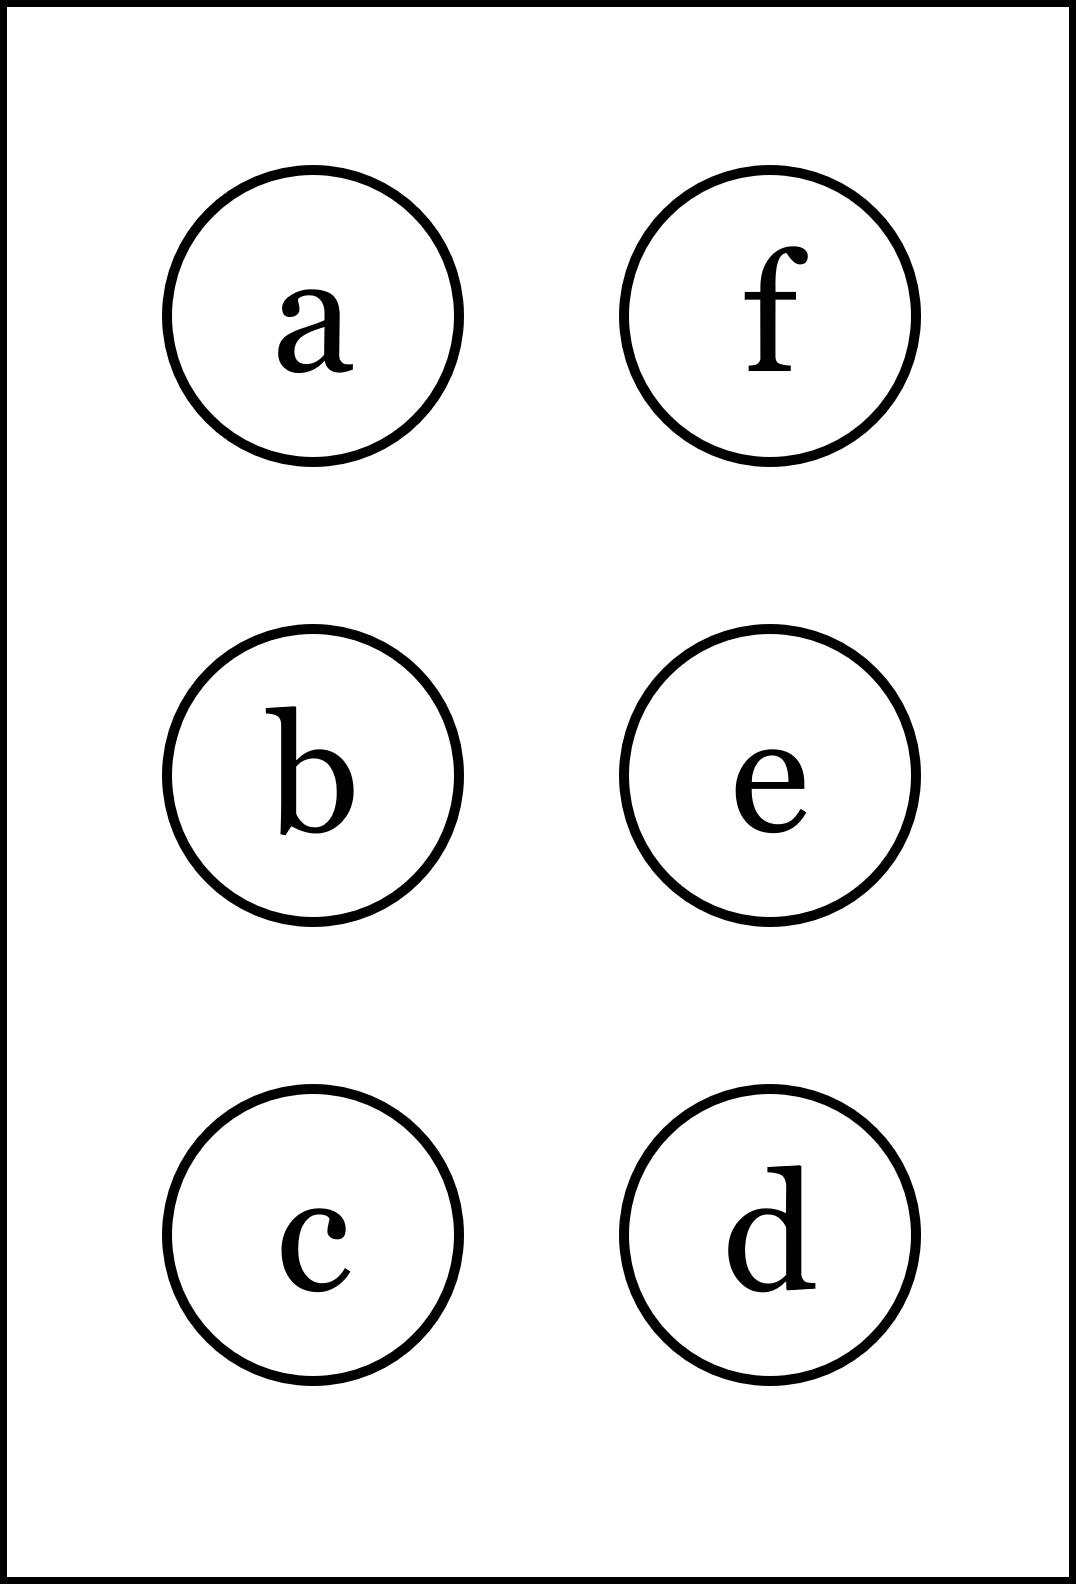
\includegraphics[height=40mm]{../images/braille.png}
{\small Písmeno Braillovej abecedy}
\end{center}
\end{minipage}
\end{center}
\end{minipage}
&
\begin{minipage}[c][104.5mm][t]{0.5\linewidth}
\begin{center}
\vspace{7mm}
{\huge Definiční obor, skupina \textit{Gamma $\gamma$} -\romannumeral4}\\[5mm]
\textit{Jméno:}\phantom{xxxxxxxxxxxxxxxxxxxxxxxxxxxxxxxxxxxxxxxxxxxxxxxxxxxxxxxxxxxxxxxxx}\\[5mm]
\begin{minipage}{0.95\linewidth}
\begin{center}
\textbf{Zjisti definiční obor} zadaných funkcí. Pokud se shoduje s tím za otazníky,\\tak napravo obarvi příslušející kroužek načerno. \textbf{Spolu odevzdejte výsledné slovo}.
\end{center}
\end{minipage}
\\[1mm]
\begin{minipage}{0.79\linewidth}
\begin{center}
\begin{varwidth}{\linewidth}
\begin{enumerate}
\normalsizerrr
\item $f(x)=\cfrac{-7x+1}{6x-1}$\quad \dotfill\; ???\;\dotfill \quad $\mathbb{R}\smallsetminus\{\nicefrac{1}{6}\}$
\item $f(x)=\cfrac{1}{4x^3-24x^2+36x-16}$\quad \dotfill\; ???\;\dotfill \quad $\mathbb{R}\smallsetminus\{1,4\}$
\item $f(x)=9\sqrt{5x+1}$\quad \dotfill\; ???\;\dotfill \quad $x\geq\nicefrac{-1}{5}$
\item $f(x)=\sqrt{-x^2-6x}$\quad \dotfill\; ???\;\dotfill \quad $x\in(-6 , 0)$
\item $f(x)=-7\ln{(-8x+3)}$\quad \dotfill\; ???\;\dotfill \quad $x>\nicefrac{3}{8}$
\item $f(x)=\ln{(x^2+x-6)}$\quad \dotfill\; ???\;\dotfill \quad $x\in(-3 , 2)$
\end{enumerate}
\end{varwidth}
\end{center}
\end{minipage}
\begin{minipage}{0.20\linewidth}
\begin{center}
{\Huge\bfseries 4.} \\[2mm]
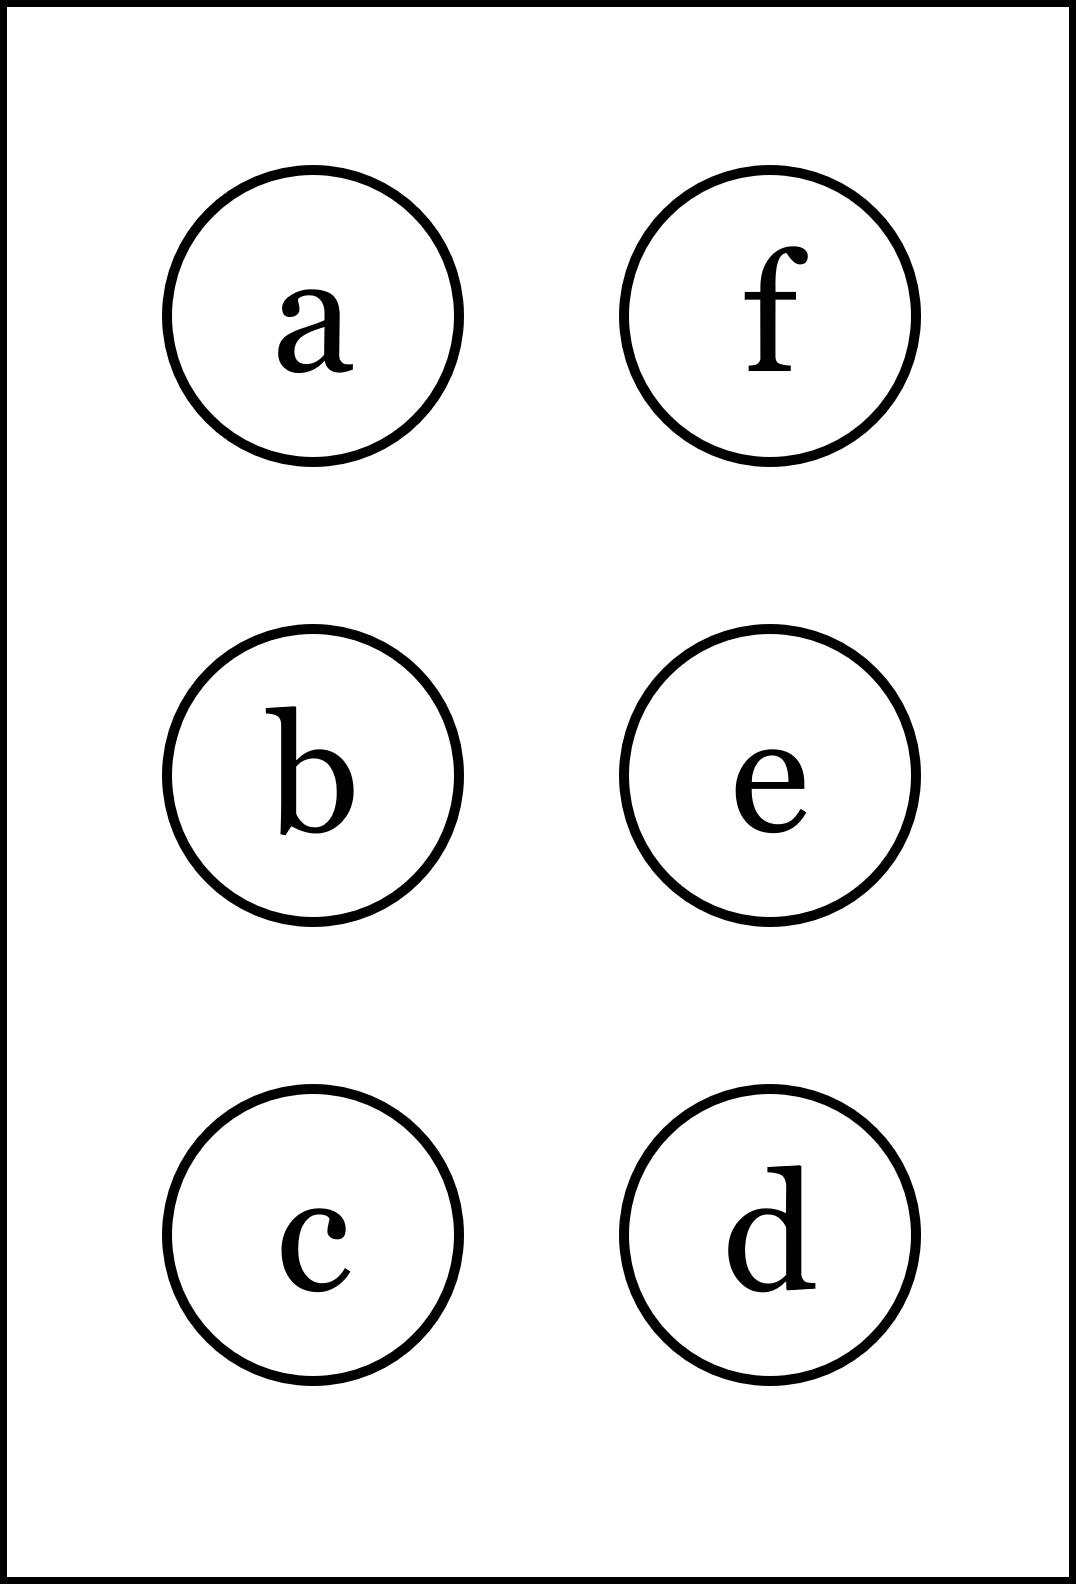
\includegraphics[height=40mm]{../images/braille.png}
{\small Písmeno Braillovej abecedy}
\end{center}
\end{minipage}
\end{center}
\end{minipage}
%
\end{tabular}
\newpage
\thispagestyle{empty}
\begin{tabular}{c:c}
\begin{minipage}[c][104.5mm][t]{0.5\linewidth}
\begin{center}
\vspace{7mm}
{\huge Definiční obor, skupina \textit{Delta $\delta$} -\romannumeral1}\\[5mm]
\textit{Jméno:}\phantom{xxxxxxxxxxxxxxxxxxxxxxxxxxxxxxxxxxxxxxxxxxxxxxxxxxxxxxxxxxxxxxxxx}\\[5mm]
\begin{minipage}{0.95\linewidth}
\begin{center}
\textbf{Zjisti definiční obor} zadaných funkcí. Pokud se shoduje s tím za otazníky,\\tak napravo obarvi příslušející kroužek načerno. \textbf{Spolu odevzdejte výsledné slovo}.
\end{center}
\end{minipage}
\\[1mm]
\begin{minipage}{0.79\linewidth}
\begin{center}
\begin{varwidth}{\linewidth}
\begin{enumerate}
\normalsizerrr
\item $f(x)=\cfrac{x-3}{4x-1}$\quad \dotfill\; ???\;\dotfill \quad $\mathbb{R}\smallsetminus\{\nicefrac{1}{4}\}$
\item $f(x)=\cfrac{1}{-2x^3+8x^2+6x-36}$\quad \dotfill\; ???\;\dotfill \quad $\mathbb{R}\smallsetminus\{-3,5,-2\}$
\item $f(x)=\sqrt{-x+1}$\quad \dotfill\; ???\;\dotfill \quad $x\leq1$
\item $f(x)=\sqrt{-x^2-2x}$\quad \dotfill\; ???\;\dotfill \quad $x\in\langle0 , 2\rangle$
\item $f(x)=-2\ln{(-2x+4)}$\quad \dotfill\; ???\;\dotfill \quad $x<2$
\item $f(x)=\ln{(x^2-13x+42)}$\quad \dotfill\; ???\;\dotfill \quad $x\in(6 , 7)$
\end{enumerate}
\end{varwidth}
\end{center}
\end{minipage}
\begin{minipage}{0.20\linewidth}
\begin{center}
{\Huge\bfseries 1.} \\[2mm]
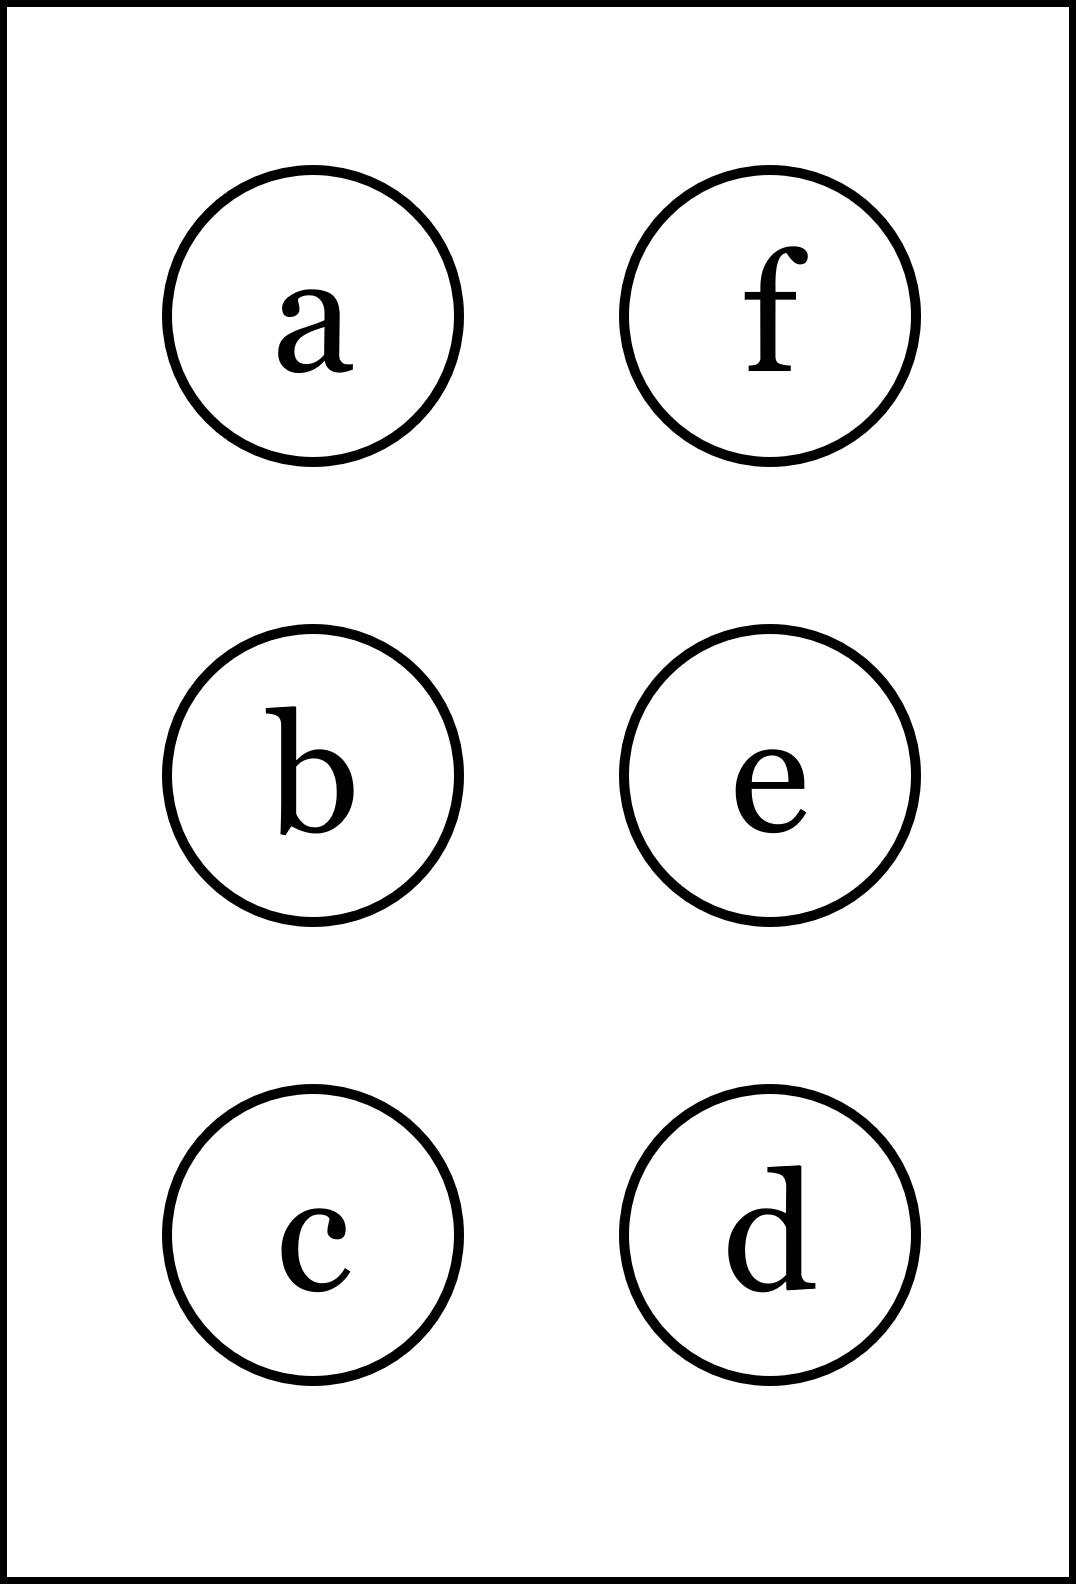
\includegraphics[height=40mm]{../images/braille.png}
{\small Písmeno Braillovej abecedy}
\end{center}
\end{minipage}
\end{center}
\end{minipage}
&
\begin{minipage}[c][104.5mm][t]{0.5\linewidth}
\begin{center}
\vspace{7mm}
{\huge Definiční obor, skupina \textit{Delta $\delta$} -\romannumeral2}\\[5mm]
\textit{Jméno:}\phantom{xxxxxxxxxxxxxxxxxxxxxxxxxxxxxxxxxxxxxxxxxxxxxxxxxxxxxxxxxxxxxxxxx}\\[5mm]
\begin{minipage}{0.95\linewidth}
\begin{center}
\textbf{Zjisti definiční obor} zadaných funkcí. Pokud se shoduje s tím za otazníky,\\tak napravo obarvi příslušející kroužek načerno. \textbf{Spolu odevzdejte výsledné slovo}.
\end{center}
\end{minipage}
\\[1mm]
\begin{minipage}{0.79\linewidth}
\begin{center}
\begin{varwidth}{\linewidth}
\begin{enumerate}
\normalsizerrr
\item $f(x)=\cfrac{-7x-2}{2x+7}$\quad \dotfill\; ???\;\dotfill \quad $\mathbb{R}\smallsetminus\{\nicefrac{-7}{2}\}$
\item $f(x)=\cfrac{1}{x^3-x^2-9x+9}$\quad \dotfill\; ???\;\dotfill \quad $\mathbb{R}\smallsetminus\{2,3\}$
\item $f(x)=-\sqrt{-9x-3}$\quad \dotfill\; ???\;\dotfill \quad $x\leq\nicefrac{-1}{3}$
\item $f(x)=\sqrt{-x^2+2x}$\quad \dotfill\; ???\;\dotfill \quad $x\in(0 , 2)$
\item $f(x)=5\ln{(x-4)}$\quad \dotfill\; ???\;\dotfill \quad $x<4$
\item $f(x)=\ln{(x^2+11x+30)}$\quad \dotfill\; ???\;\dotfill \quad $x\in(-6 , -5)$
\end{enumerate}
\end{varwidth}
\end{center}
\end{minipage}
\begin{minipage}{0.20\linewidth}
\begin{center}
{\Huge\bfseries 2.} \\[2mm]
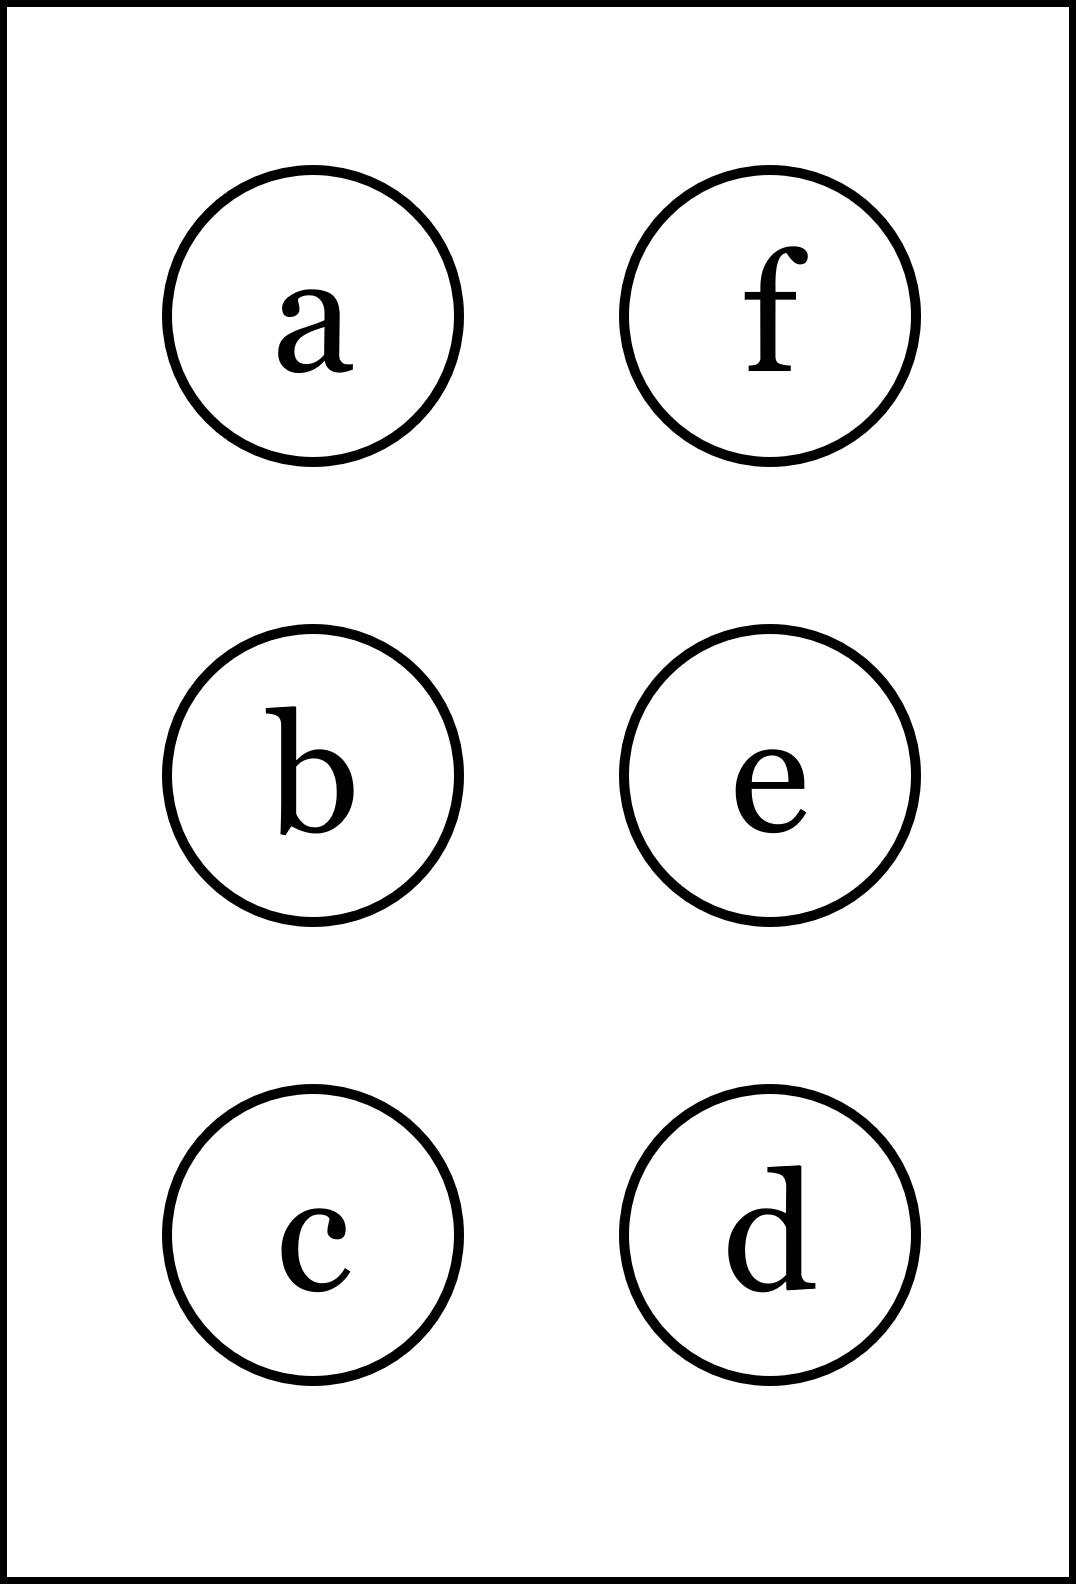
\includegraphics[height=40mm]{../images/braille.png}
{\small Písmeno Braillovej abecedy}
\end{center}
\end{minipage}
\end{center}
\end{minipage}
\\ \hdashline
\begin{minipage}[c][104.5mm][t]{0.5\linewidth}
\begin{center}
\vspace{7mm}
{\huge Definiční obor, skupina \textit{Delta $\delta$} -\romannumeral3}\\[5mm]
\textit{Jméno:}\phantom{xxxxxxxxxxxxxxxxxxxxxxxxxxxxxxxxxxxxxxxxxxxxxxxxxxxxxxxxxxxxxxxxx}\\[5mm]
\begin{minipage}{0.95\linewidth}
\begin{center}
\textbf{Zjisti definiční obor} zadaných funkcí. Pokud se shoduje s tím za otazníky,\\tak napravo obarvi příslušející kroužek načerno. \textbf{Spolu odevzdejte výsledné slovo}.
\end{center}
\end{minipage}
\\[1mm]
\begin{minipage}{0.79\linewidth}
\begin{center}
\begin{varwidth}{\linewidth}
\begin{enumerate}
\normalsizerrr
\item $f(x)=\cfrac{-5x+6}{-5x+2}$\quad \dotfill\; ???\;\dotfill \quad $\mathbb{R}\smallsetminus\{\nicefrac{2}{5}\}$
\item $f(x)=\cfrac{1}{4x^3+16x^2-4x-16}$\quad \dotfill\; ???\;\dotfill \quad $\mathbb{R}\smallsetminus\{1,-4,-1\}$
\item $f(x)=-\sqrt{x+3}$\quad \dotfill\; ???\;\dotfill \quad $x\geq-3$
\item $f(x)=\sqrt{-x^2-2x}$\quad \dotfill\; ???\;\dotfill \quad $x\in(-2 , 0)$
\item $f(x)=5\ln{(-2x+3)}$\quad \dotfill\; ???\;\dotfill \quad $x<\nicefrac{3}{2}$
\item $f(x)=\ln{(x^2+10x+24)}$\quad \dotfill\; ???\;\dotfill \quad $x\in(-\infty , -6)\cup(-4 , \infty)$
\end{enumerate}
\end{varwidth}
\end{center}
\end{minipage}
\begin{minipage}{0.20\linewidth}
\begin{center}
{\Huge\bfseries 3.} \\[2mm]
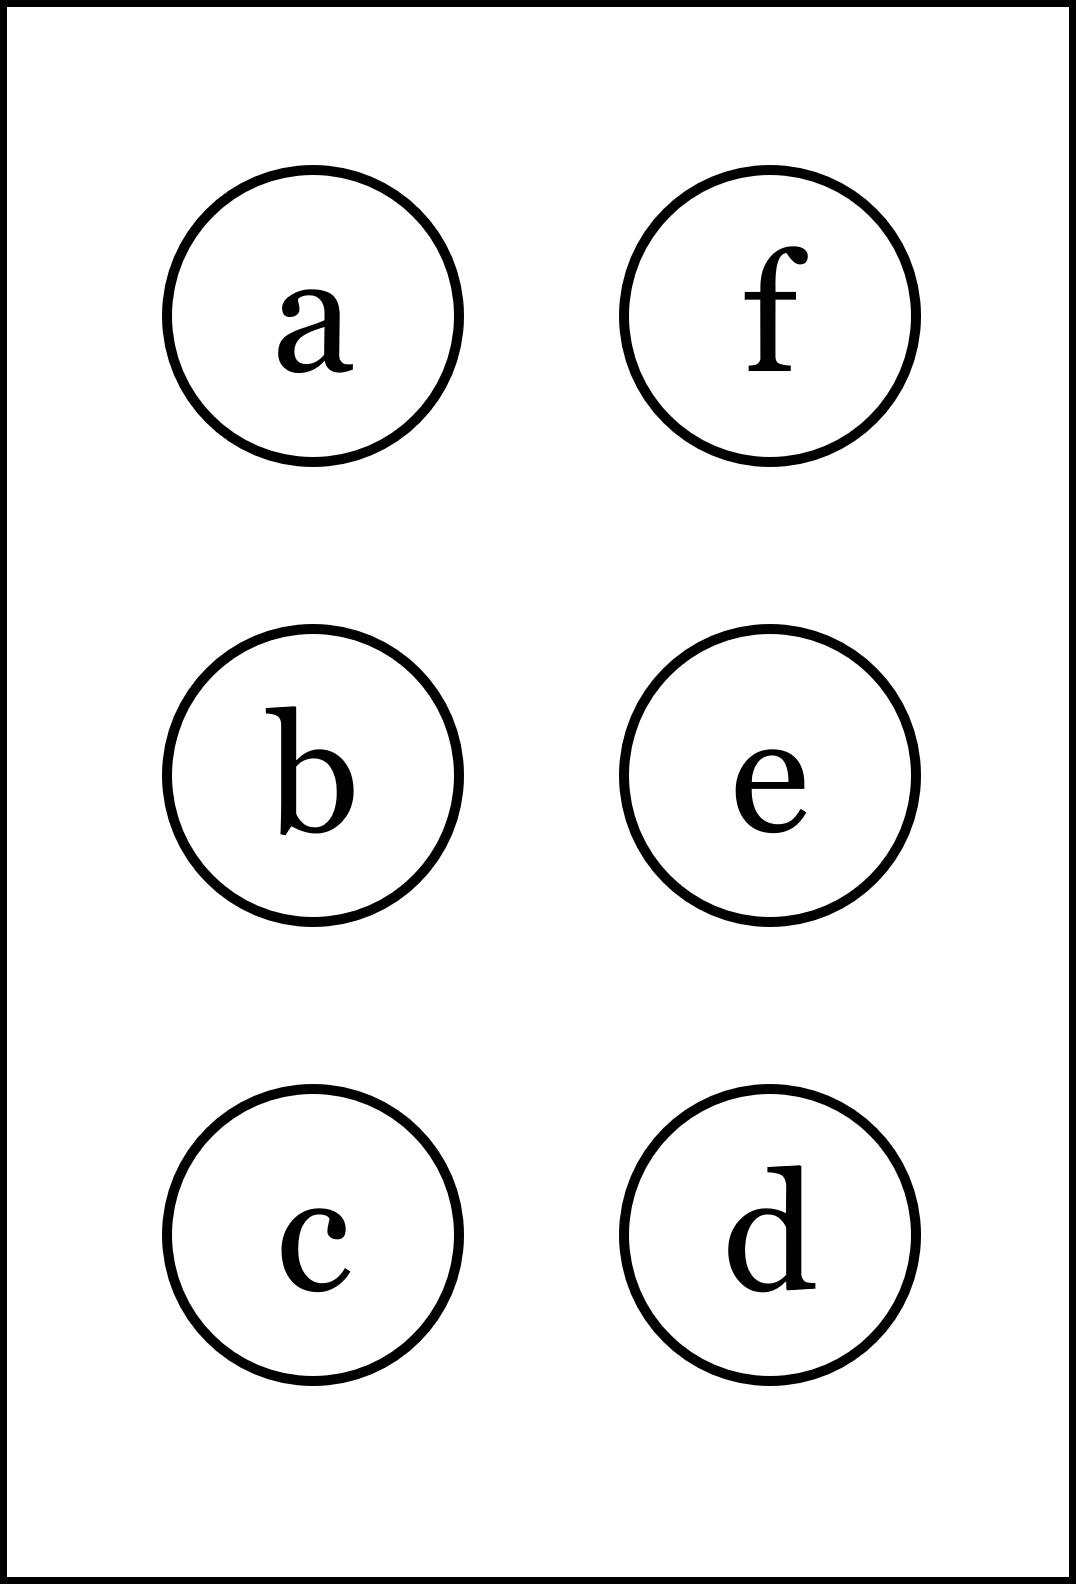
\includegraphics[height=40mm]{../images/braille.png}
{\small Písmeno Braillovej abecedy}
\end{center}
\end{minipage}
\end{center}
\end{minipage}
&
\begin{minipage}[c][104.5mm][t]{0.5\linewidth}
\begin{center}
\vspace{7mm}
{\huge Definiční obor, skupina \textit{Delta $\delta$} -\romannumeral4}\\[5mm]
\textit{Jméno:}\phantom{xxxxxxxxxxxxxxxxxxxxxxxxxxxxxxxxxxxxxxxxxxxxxxxxxxxxxxxxxxxxxxxxx}\\[5mm]
\begin{minipage}{0.95\linewidth}
\begin{center}
\textbf{Zjisti definiční obor} zadaných funkcí. Pokud se shoduje s tím za otazníky,\\tak napravo obarvi příslušející kroužek načerno. \textbf{Spolu odevzdejte výsledné slovo}.
\end{center}
\end{minipage}
\\[1mm]
\begin{minipage}{0.79\linewidth}
\begin{center}
\begin{varwidth}{\linewidth}
\begin{enumerate}
\normalsizerrr
\item $f(x)=\cfrac{3x+4}{9x+4}$\quad \dotfill\; ???\;\dotfill \quad $\mathbb{R}\smallsetminus\{\nicefrac{-4}{9}\}$
\item $f(x)=\cfrac{1}{-3x^3-27x^2-69x-45}$\quad \dotfill\; ???\;\dotfill \quad $\mathbb{R}\smallsetminus\{1,-4,-3\}$
\item $f(x)=-5\sqrt{-8x+3}$\quad \dotfill\; ???\;\dotfill \quad $x\leq\nicefrac{3}{8}$
\item $f(x)=\sqrt{-x^2-4x}$\quad \dotfill\; ???\;\dotfill \quad $x\in\langle0 , 4\rangle$
\item $f(x)=-6\ln{(4x-4)}$\quad \dotfill\; ???\;\dotfill \quad $x>1$
\item $f(x)=\ln{(x^2-4x-5)}$\quad \dotfill\; ???\;\dotfill \quad $x\in(-1 , 5)$
\end{enumerate}
\end{varwidth}
\end{center}
\end{minipage}
\begin{minipage}{0.20\linewidth}
\begin{center}
{\Huge\bfseries 4.} \\[2mm]
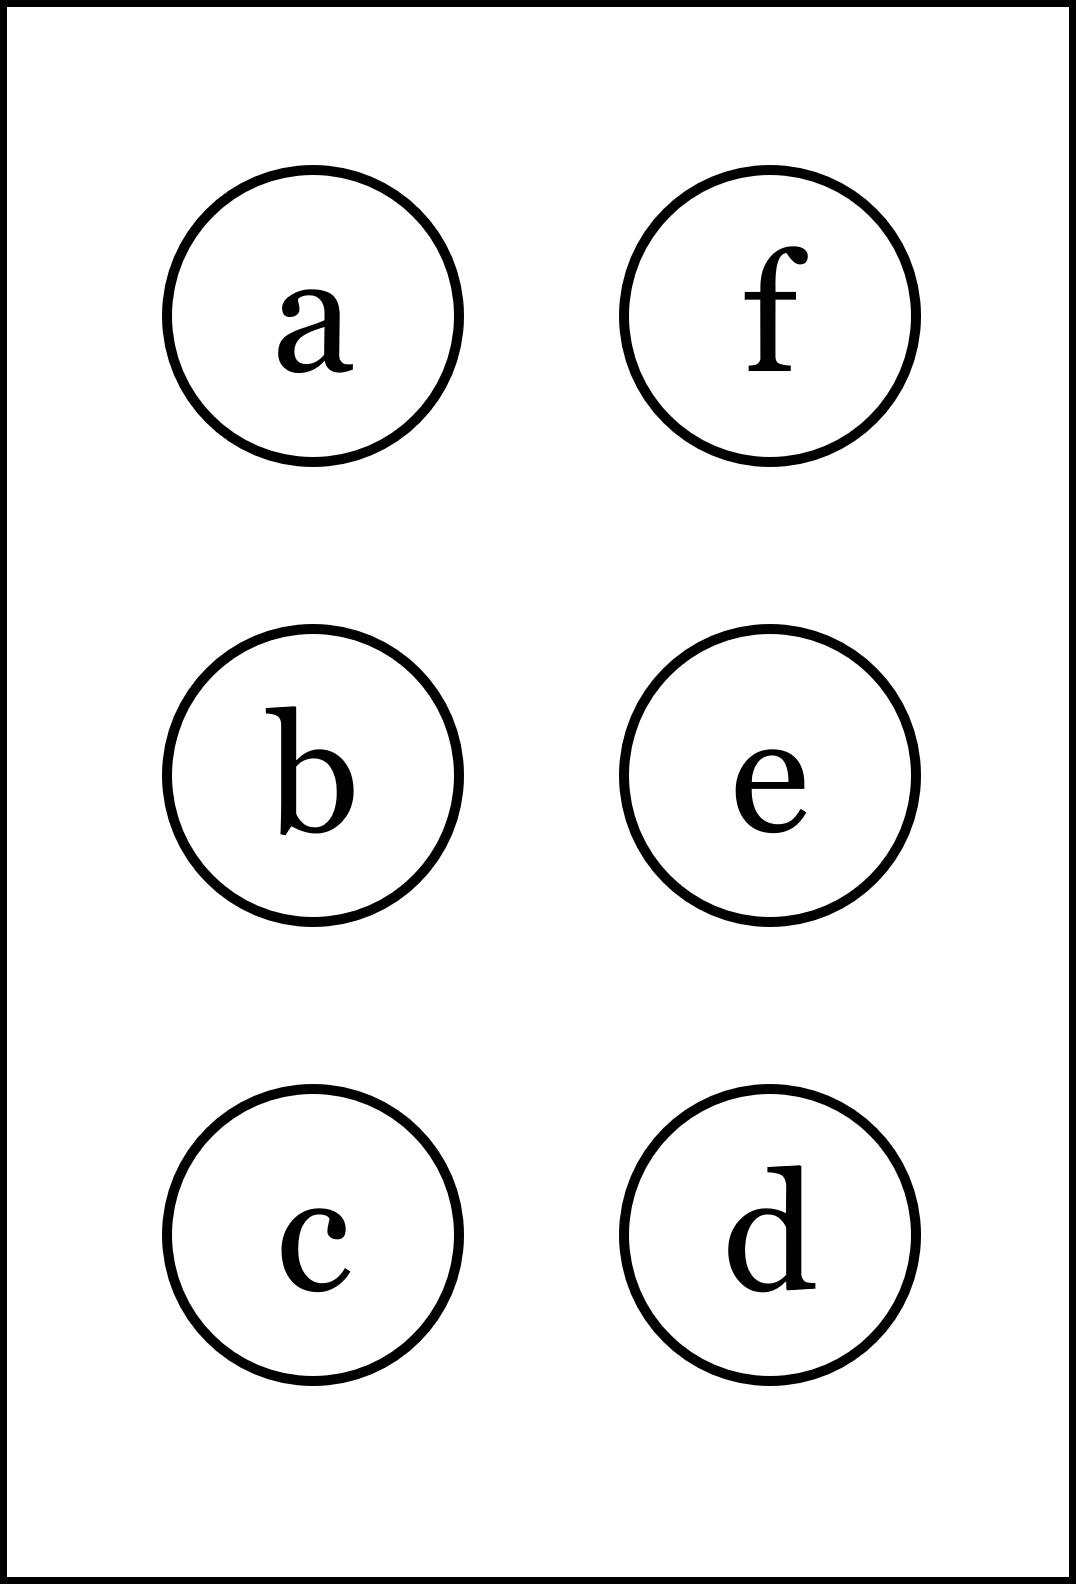
\includegraphics[height=40mm]{../images/braille.png}
{\small Písmeno Braillovej abecedy}
\end{center}
\end{minipage}
\end{center}
\end{minipage}
%
\end{tabular}
\newpage
\thispagestyle{empty}
\begin{tabular}{c:c}
\begin{minipage}[c][104.5mm][t]{0.5\linewidth}
\begin{center}
\vspace{7mm}
{\huge Definiční obor, skupina \textit{Epsilon $\epsilon$} -\romannumeral1}\\[5mm]
\textit{Jméno:}\phantom{xxxxxxxxxxxxxxxxxxxxxxxxxxxxxxxxxxxxxxxxxxxxxxxxxxxxxxxxxxxxxxxxx}\\[5mm]
\begin{minipage}{0.95\linewidth}
\begin{center}
\textbf{Zjisti definiční obor} zadaných funkcí. Pokud se shoduje s tím za otazníky,\\tak napravo obarvi příslušející kroužek načerno. \textbf{Spolu odevzdejte výsledné slovo}.
\end{center}
\end{minipage}
\\[1mm]
\begin{minipage}{0.79\linewidth}
\begin{center}
\begin{varwidth}{\linewidth}
\begin{enumerate}
\normalsizerrr
\item $f(x)=\cfrac{-6x-2}{-x-4}$\quad \dotfill\; ???\;\dotfill \quad $\mathbb{R}\smallsetminus\{-4\}$
\item $f(x)=\cfrac{1}{-x^3-4x^2-5x-2}$\quad \dotfill\; ???\;\dotfill \quad $\mathbb{R}\smallsetminus\{1,2,-1\}$
\item $f(x)=-\sqrt{-2x+1}$\quad \dotfill\; ???\;\dotfill \quad $x\geq\nicefrac{1}{2}$
\item $f(x)=\sqrt{-x^2-7x}$\quad \dotfill\; ???\;\dotfill \quad $x\in(-7 , 0)$
\item $f(x)=-8\ln{(2x-4)}$\quad \dotfill\; ???\;\dotfill \quad $x<2$
\item $f(x)=\ln{(x^2+10x+24)}$\quad \dotfill\; ???\;\dotfill \quad $x\in(-\infty , -6)\cup(-4 , \infty)$
\end{enumerate}
\end{varwidth}
\end{center}
\end{minipage}
\begin{minipage}{0.20\linewidth}
\begin{center}
{\Huge\bfseries 1.} \\[2mm]
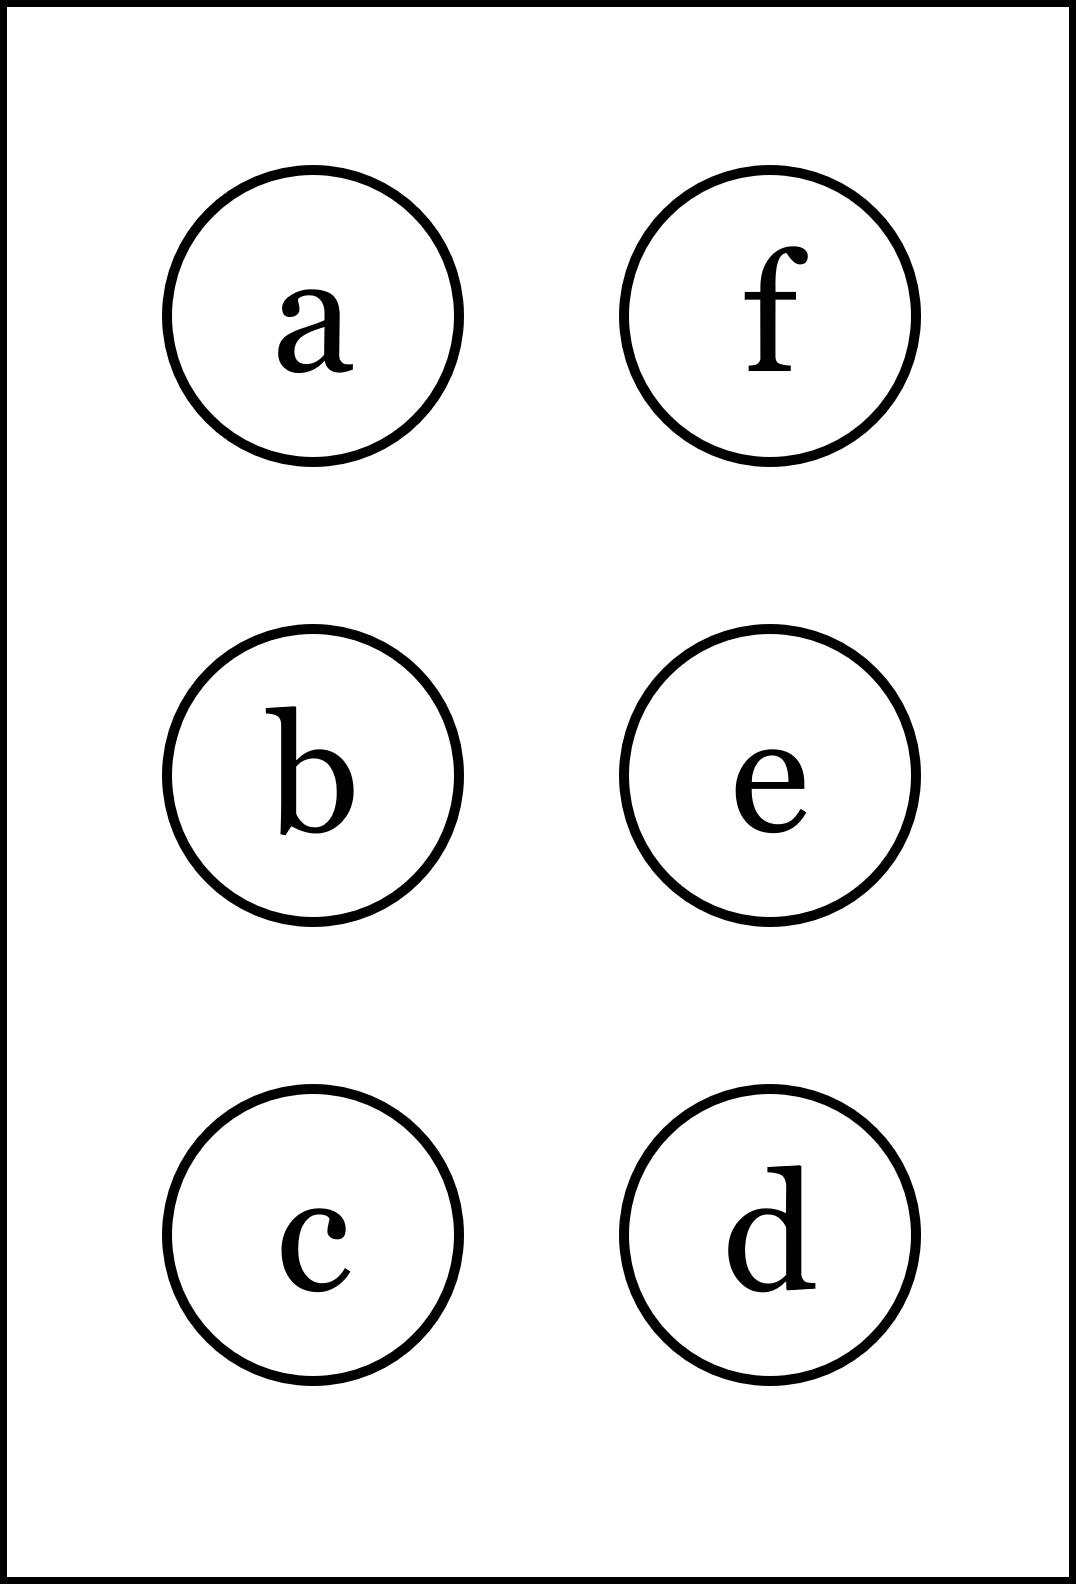
\includegraphics[height=40mm]{../images/braille.png}
{\small Písmeno Braillovej abecedy}
\end{center}
\end{minipage}
\end{center}
\end{minipage}
&
\begin{minipage}[c][104.5mm][t]{0.5\linewidth}
\begin{center}
\vspace{7mm}
{\huge Definiční obor, skupina \textit{Epsilon $\epsilon$} -\romannumeral2}\\[5mm]
\textit{Jméno:}\phantom{xxxxxxxxxxxxxxxxxxxxxxxxxxxxxxxxxxxxxxxxxxxxxxxxxxxxxxxxxxxxxxxxx}\\[5mm]
\begin{minipage}{0.95\linewidth}
\begin{center}
\textbf{Zjisti definiční obor} zadaných funkcí. Pokud se shoduje s tím za otazníky,\\tak napravo obarvi příslušející kroužek načerno. \textbf{Spolu odevzdejte výsledné slovo}.
\end{center}
\end{minipage}
\\[1mm]
\begin{minipage}{0.79\linewidth}
\begin{center}
\begin{varwidth}{\linewidth}
\begin{enumerate}
\normalsizerrr
\item $f(x)=\cfrac{7x+8}{8x-6}$\quad \dotfill\; ???\;\dotfill \quad $\mathbb{R}\smallsetminus\{\nicefrac{3}{4}\}$
\item $f(x)=\cfrac{1}{-4x^3-16x^2-20x-8}$\quad \dotfill\; ???\;\dotfill \quad $\mathbb{R}\smallsetminus\{1,-3,-1\}$
\item $f(x)=-4\sqrt{2x+4}$\quad \dotfill\; ???\;\dotfill \quad $x\geq2$
\item $f(x)=\sqrt{-x^2-4x}$\quad \dotfill\; ???\;\dotfill \quad $x\in\langle0 , 4\rangle$
\item $f(x)=-6\ln{(4x-3)}$\quad \dotfill\; ???\;\dotfill \quad $x>\nicefrac{3}{4}$
\item $f(x)=\ln{(x^2+14x+48)}$\quad \dotfill\; ???\;\dotfill \quad $x\in(-8 , -6)$
\end{enumerate}
\end{varwidth}
\end{center}
\end{minipage}
\begin{minipage}{0.20\linewidth}
\begin{center}
{\Huge\bfseries 2.} \\[2mm]
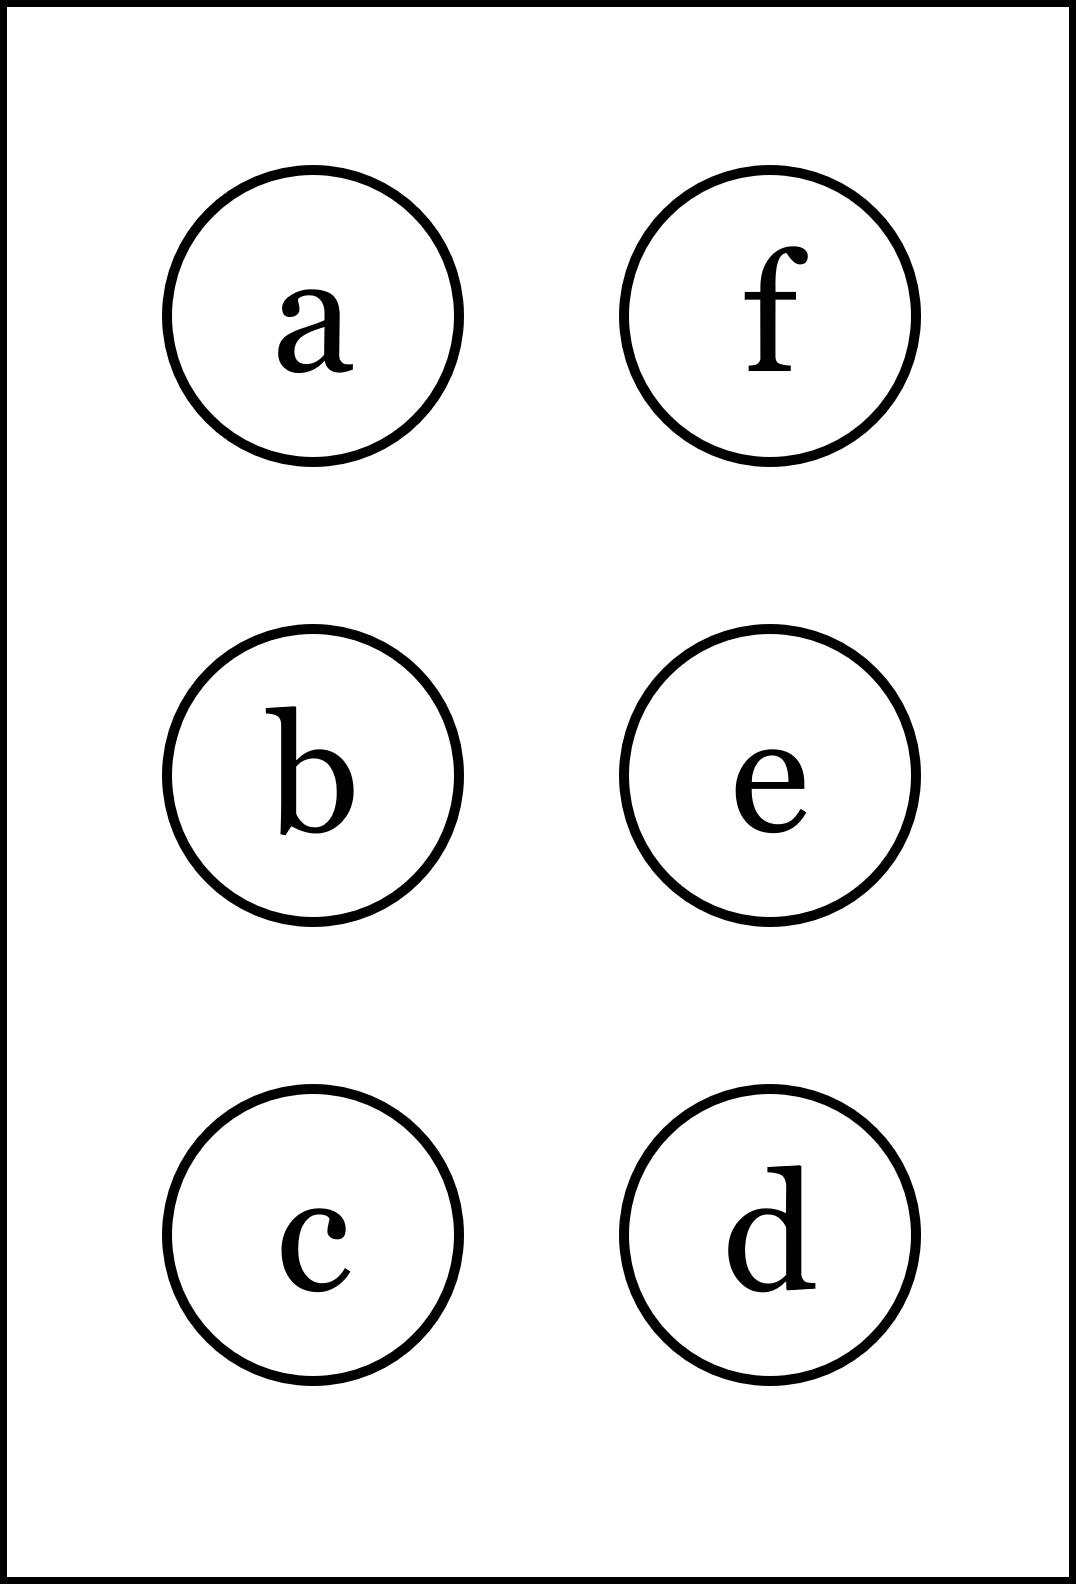
\includegraphics[height=40mm]{../images/braille.png}
{\small Písmeno Braillovej abecedy}
\end{center}
\end{minipage}
\end{center}
\end{minipage}
\\ \hdashline
\begin{minipage}[c][104.5mm][t]{0.5\linewidth}
\begin{center}
\vspace{7mm}
{\huge Definiční obor, skupina \textit{Epsilon $\epsilon$} -\romannumeral3}\\[5mm]
\textit{Jméno:}\phantom{xxxxxxxxxxxxxxxxxxxxxxxxxxxxxxxxxxxxxxxxxxxxxxxxxxxxxxxxxxxxxxxxx}\\[5mm]
\begin{minipage}{0.95\linewidth}
\begin{center}
\textbf{Zjisti definiční obor} zadaných funkcí. Pokud se shoduje s tím za otazníky,\\tak napravo obarvi příslušející kroužek načerno. \textbf{Spolu odevzdejte výsledné slovo}.
\end{center}
\end{minipage}
\\[1mm]
\begin{minipage}{0.79\linewidth}
\begin{center}
\begin{varwidth}{\linewidth}
\begin{enumerate}
\normalsizerrr
\item $f(x)=\cfrac{2x-3}{3x-2}$\quad \dotfill\; ???\;\dotfill \quad $\mathbb{R}\smallsetminus\{\nicefrac{2}{3}\}$
\item $f(x)=\cfrac{1}{-x^3-8x^2-21x-18}$\quad \dotfill\; ???\;\dotfill \quad $\mathbb{R}\smallsetminus\{2,-3,-1\}$
\item $f(x)=5\sqrt{-9x+3}$\quad \dotfill\; ???\;\dotfill \quad $x\leq\nicefrac{1}{3}$
\item $f(x)=\sqrt{-x^2+2x}$\quad \dotfill\; ???\;\dotfill \quad $x\in(0 , 2)$
\item $f(x)=-9\ln{(-5x-1)}$\quad \dotfill\; ???\;\dotfill \quad $x<\nicefrac{-1}{5}$
\item $f(x)=\ln{(x^2+3x+2)}$\quad \dotfill\; ???\;\dotfill \quad $x\in(-\infty , -2)\cup(-1 , \infty)$
\end{enumerate}
\end{varwidth}
\end{center}
\end{minipage}
\begin{minipage}{0.20\linewidth}
\begin{center}
{\Huge\bfseries 3.} \\[2mm]
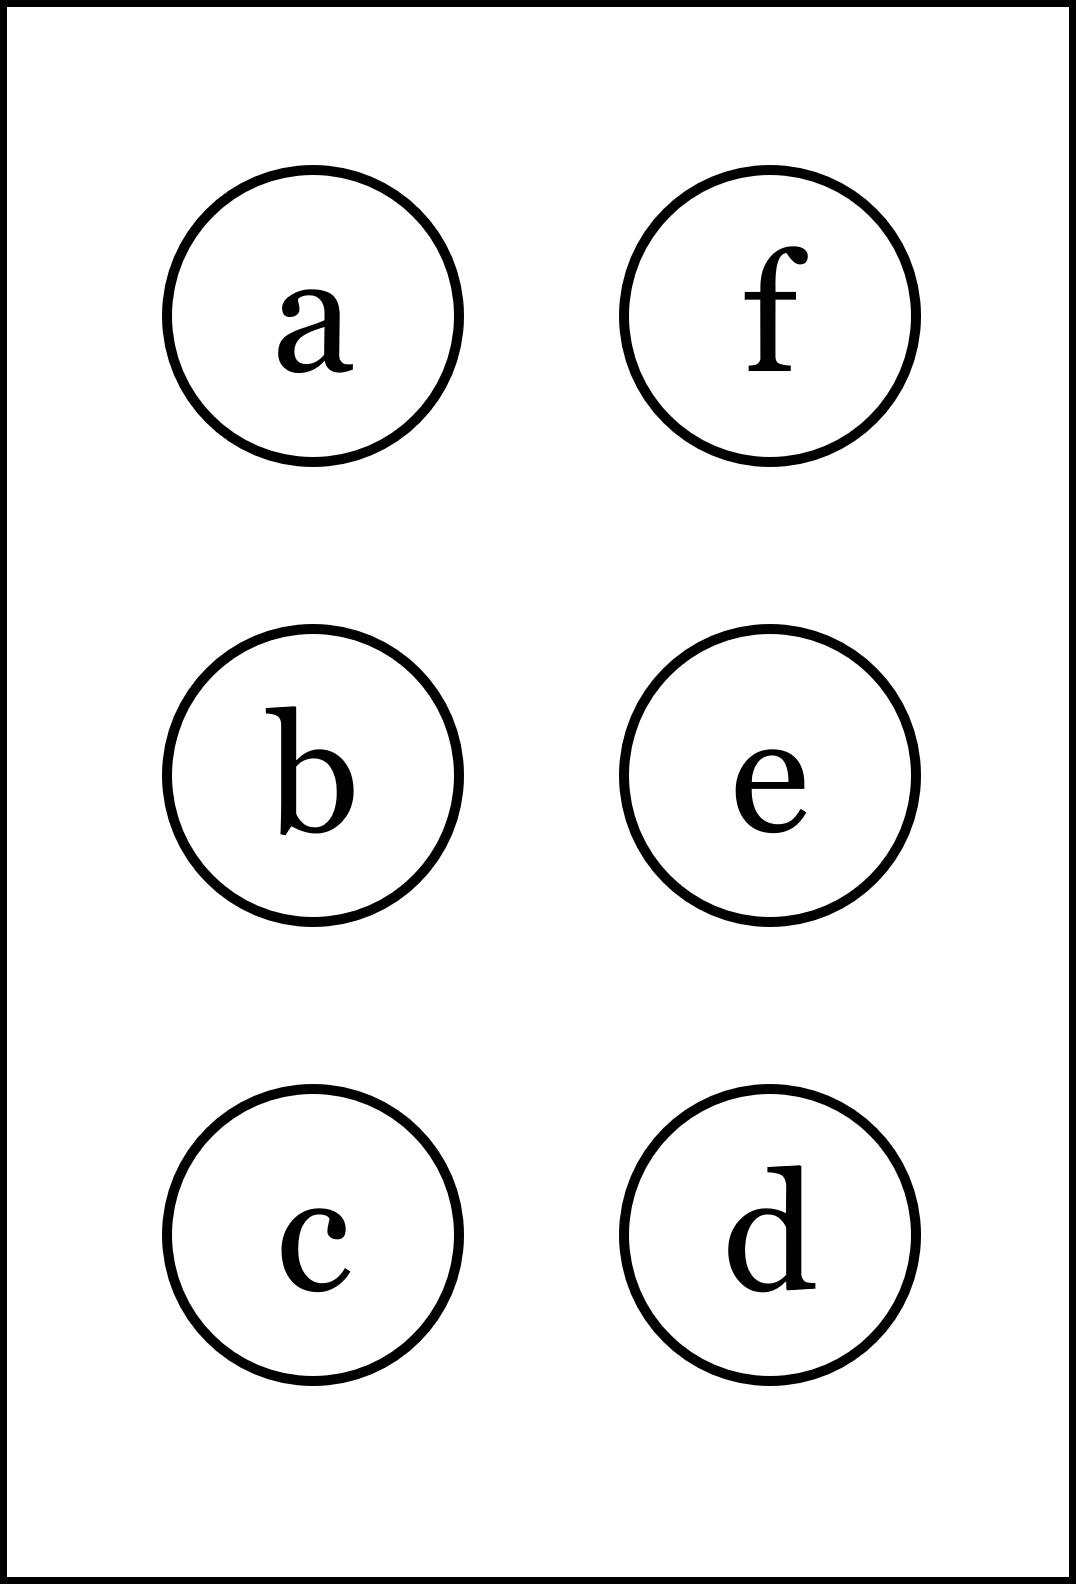
\includegraphics[height=40mm]{../images/braille.png}
{\small Písmeno Braillovej abecedy}
\end{center}
\end{minipage}
\end{center}
\end{minipage}
&
\begin{minipage}[c][104.5mm][t]{0.5\linewidth}
\begin{center}
\vspace{7mm}
{\huge Definiční obor, skupina \textit{Epsilon $\epsilon$} -\romannumeral4}\\[5mm]
\textit{Jméno:}\phantom{xxxxxxxxxxxxxxxxxxxxxxxxxxxxxxxxxxxxxxxxxxxxxxxxxxxxxxxxxxxxxxxxx}\\[5mm]
\begin{minipage}{0.95\linewidth}
\begin{center}
\textbf{Zjisti definiční obor} zadaných funkcí. Pokud se shoduje s tím za otazníky,\\tak napravo obarvi příslušející kroužek načerno. \textbf{Spolu odevzdejte výsledné slovo}.
\end{center}
\end{minipage}
\\[1mm]
\begin{minipage}{0.79\linewidth}
\begin{center}
\begin{varwidth}{\linewidth}
\begin{enumerate}
\normalsizerrr
\item $f(x)=\cfrac{-5x+6}{2x-2}$\quad \dotfill\; ???\;\dotfill \quad $\mathbb{R}\smallsetminus\{1\}$
\item $f(x)=\cfrac{1}{-6x^3+36x^2-54x+24}$\quad \dotfill\; ???\;\dotfill \quad $\mathbb{R}\smallsetminus\{1,3,-1\}$
\item $f(x)=3\sqrt{3x+4}$\quad \dotfill\; ???\;\dotfill \quad $x\geq\nicefrac{4}{3}$
\item $f(x)=\sqrt{-x^2-x}$\quad \dotfill\; ???\;\dotfill \quad $x\in\langle0 , 1\rangle$
\item $f(x)=3\ln{(8x-2)}$\quad \dotfill\; ???\;\dotfill \quad $x>\nicefrac{-1}{4}$
\item $f(x)=\ln{(x^2+2x-8)}$\quad \dotfill\; ???\;\dotfill \quad $x\in(-4 , 2)$
\end{enumerate}
\end{varwidth}
\end{center}
\end{minipage}
\begin{minipage}{0.20\linewidth}
\begin{center}
{\Huge\bfseries 4.} \\[2mm]
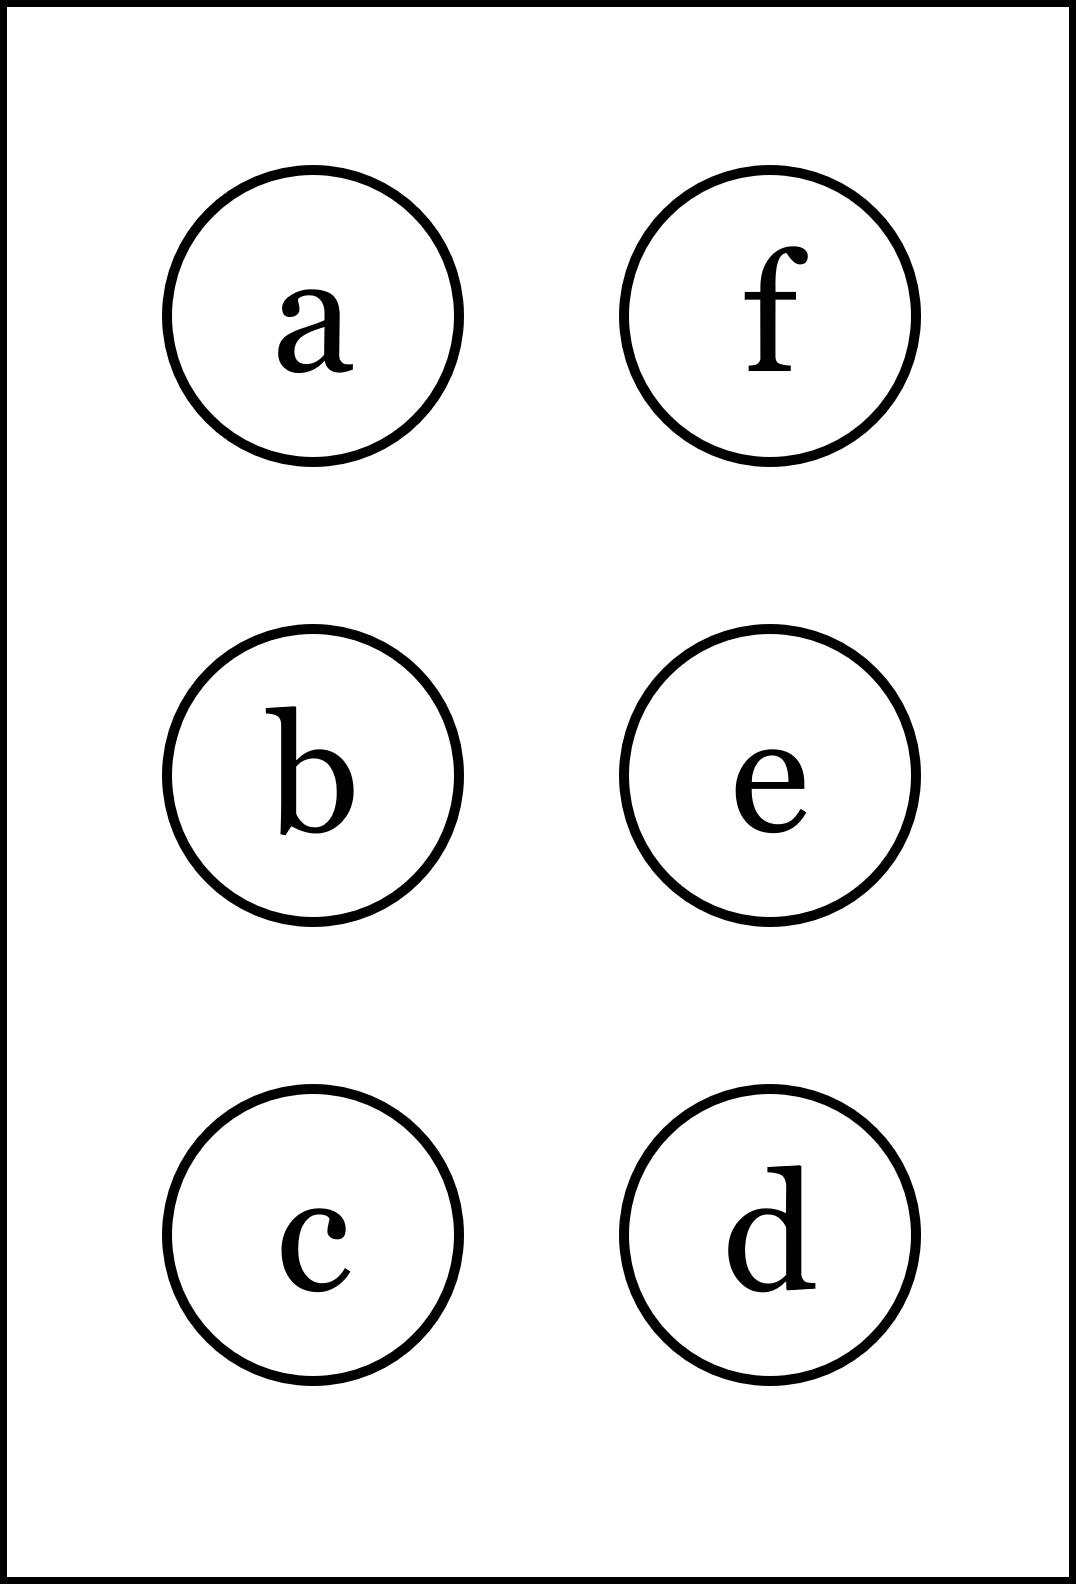
\includegraphics[height=40mm]{../images/braille.png}
{\small Písmeno Braillovej abecedy}
\end{center}
\end{minipage}
\end{center}
\end{minipage}
%
\end{tabular}
\newpage
\thispagestyle{empty}
\begin{tabular}{c:c}
\begin{minipage}[c][104.5mm][t]{0.5\linewidth}
\begin{center}
\vspace{7mm}
{\huge Definiční obor, skupina \textit{Zeta $\zeta$} -\romannumeral1}\\[5mm]
\textit{Jméno:}\phantom{xxxxxxxxxxxxxxxxxxxxxxxxxxxxxxxxxxxxxxxxxxxxxxxxxxxxxxxxxxxxxxxxx}\\[5mm]
\begin{minipage}{0.95\linewidth}
\begin{center}
\textbf{Zjisti definiční obor} zadaných funkcí. Pokud se shoduje s tím za otazníky,\\tak napravo obarvi příslušející kroužek načerno. \textbf{Spolu odevzdejte výsledné slovo}.
\end{center}
\end{minipage}
\\[1mm]
\begin{minipage}{0.79\linewidth}
\begin{center}
\begin{varwidth}{\linewidth}
\begin{enumerate}
\normalsizerrr
\item $f(x)=\cfrac{5x-1}{-6x+3}$\quad \dotfill\; ???\;\dotfill \quad $\mathbb{R}\smallsetminus\{\nicefrac{1}{2}\}$
\item $f(x)=\cfrac{1}{4x^3-12x-8}$\quad \dotfill\; ???\;\dotfill \quad $\mathbb{R}\smallsetminus\{2,-1\}$
\item $f(x)=3\sqrt{-7x+6}$\quad \dotfill\; ???\;\dotfill \quad $x\leq\nicefrac{6}{7}$
\item $f(x)=\sqrt{-x^2+x}$\quad \dotfill\; ???\;\dotfill \quad $x\in\langle0 , 1\rangle$
\item $f(x)=2\ln{(5x-8)}$\quad \dotfill\; ???\;\dotfill \quad $x>\nicefrac{8}{5}$
\item $f(x)=\ln{(x^2+9x+8)}$\quad \dotfill\; ???\;\dotfill \quad $x\in(-8 , -1)$
\end{enumerate}
\end{varwidth}
\end{center}
\end{minipage}
\begin{minipage}{0.20\linewidth}
\begin{center}
{\Huge\bfseries 1.} \\[2mm]
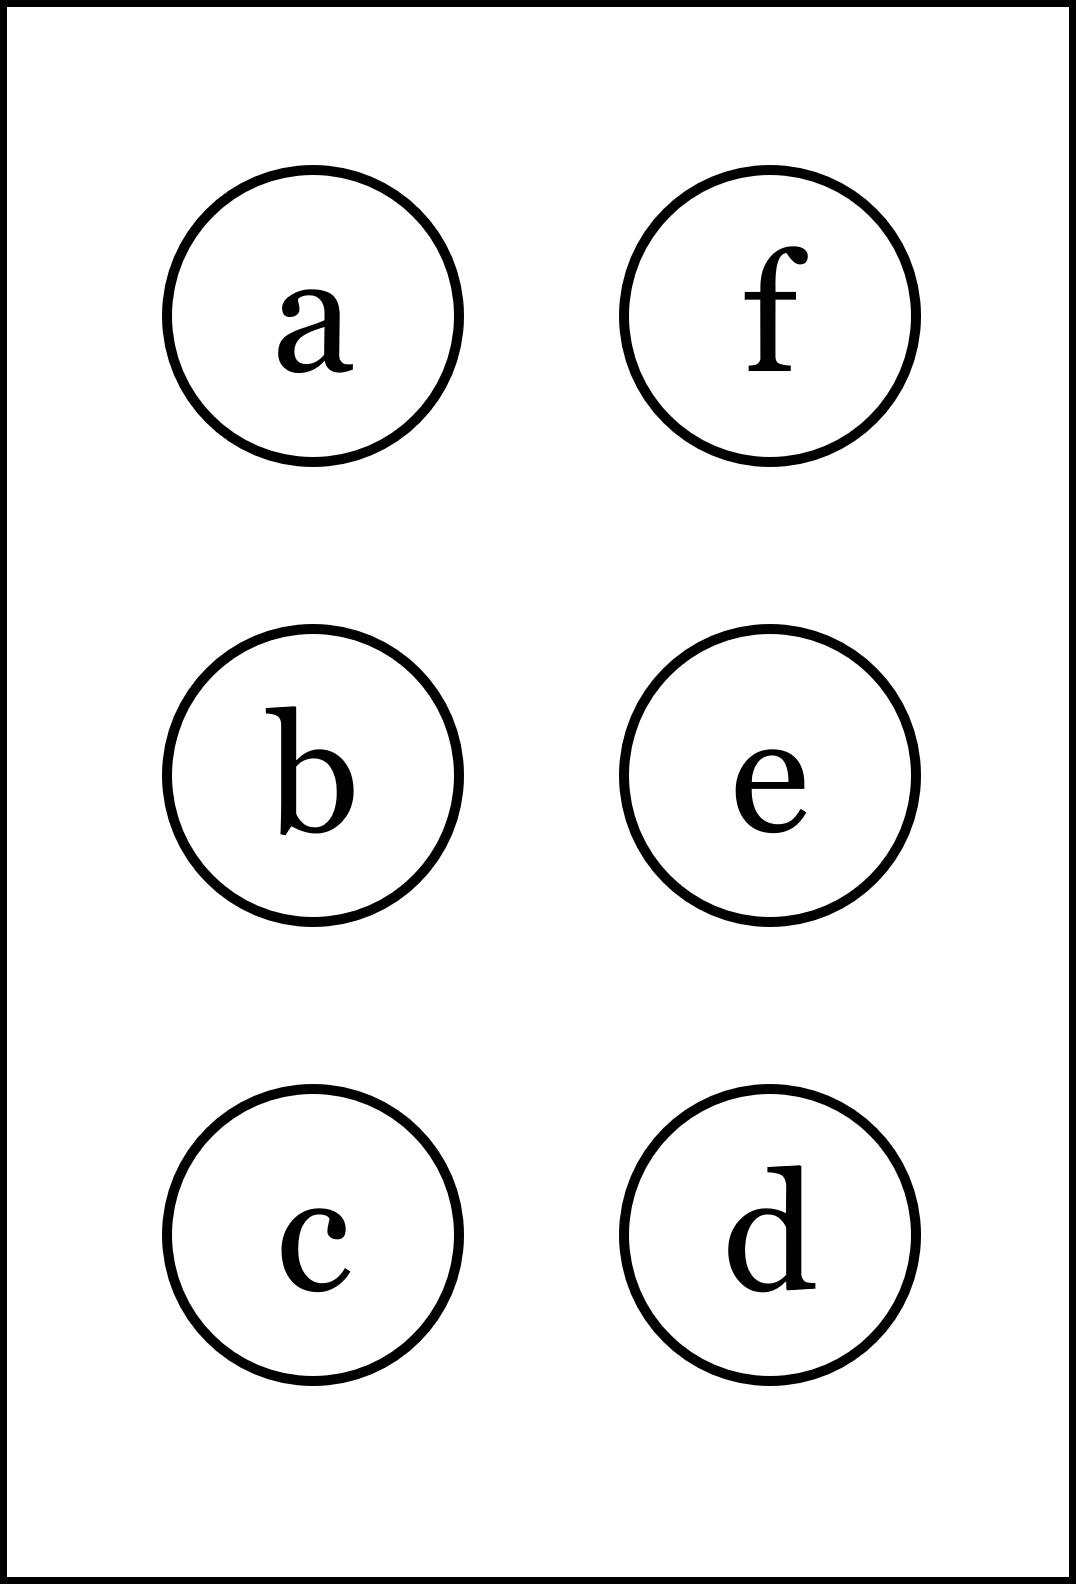
\includegraphics[height=40mm]{../images/braille.png}
{\small Písmeno Braillovej abecedy}
\end{center}
\end{minipage}
\end{center}
\end{minipage}
&
\begin{minipage}[c][104.5mm][t]{0.5\linewidth}
\begin{center}
\vspace{7mm}
{\huge Definiční obor, skupina \textit{Zeta $\zeta$} -\romannumeral2}\\[5mm]
\textit{Jméno:}\phantom{xxxxxxxxxxxxxxxxxxxxxxxxxxxxxxxxxxxxxxxxxxxxxxxxxxxxxxxxxxxxxxxxx}\\[5mm]
\begin{minipage}{0.95\linewidth}
\begin{center}
\textbf{Zjisti definiční obor} zadaných funkcí. Pokud se shoduje s tím za otazníky,\\tak napravo obarvi příslušející kroužek načerno. \textbf{Spolu odevzdejte výsledné slovo}.
\end{center}
\end{minipage}
\\[1mm]
\begin{minipage}{0.79\linewidth}
\begin{center}
\begin{varwidth}{\linewidth}
\begin{enumerate}
\normalsizerrr
\item $f(x)=\cfrac{8x+8}{x-1}$\quad \dotfill\; ???\;\dotfill \quad $\mathbb{R}\smallsetminus\{1\}$
\item $f(x)=\cfrac{1}{3x^3-21x^2+33x-15}$\quad \dotfill\; ???\;\dotfill \quad $\mathbb{R}\smallsetminus\{1,-1,7\}$
\item $f(x)=-3\sqrt{-4x-6}$\quad \dotfill\; ???\;\dotfill \quad $x\leq\nicefrac{-3}{2}$
\item $f(x)=\sqrt{-x^2+4x}$\quad \dotfill\; ???\;\dotfill \quad $x\in(0 , 4)$
\item $f(x)=4\ln{(-5x-4)}$\quad \dotfill\; ???\;\dotfill \quad $x<\nicefrac{-4}{5}$
\item $f(x)=\ln{(x^2+5x-14)}$\quad \dotfill\; ???\;\dotfill \quad $x\in(-7 , 2)$
\end{enumerate}
\end{varwidth}
\end{center}
\end{minipage}
\begin{minipage}{0.20\linewidth}
\begin{center}
{\Huge\bfseries 2.} \\[2mm]
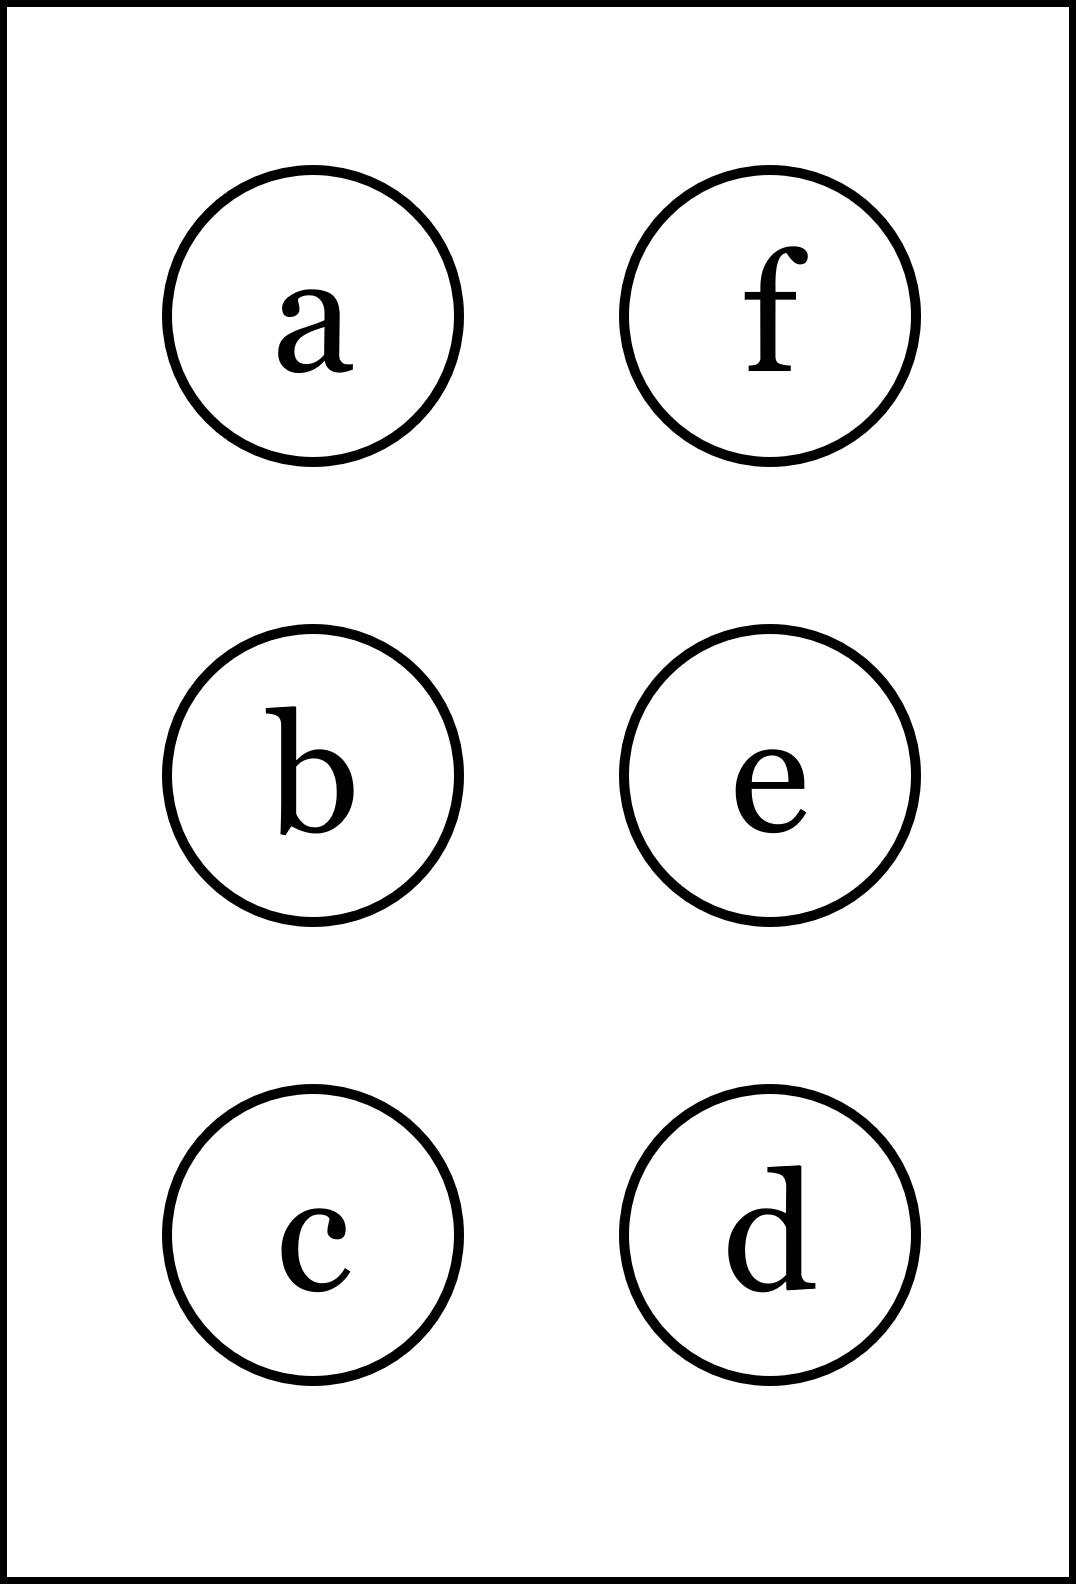
\includegraphics[height=40mm]{../images/braille.png}
{\small Písmeno Braillovej abecedy}
\end{center}
\end{minipage}
\end{center}
\end{minipage}
\\ \hdashline
\begin{minipage}[c][104.5mm][t]{0.5\linewidth}
\begin{center}
\vspace{7mm}
{\huge Definiční obor, skupina \textit{Zeta $\zeta$} -\romannumeral3}\\[5mm]
\textit{Jméno:}\phantom{xxxxxxxxxxxxxxxxxxxxxxxxxxxxxxxxxxxxxxxxxxxxxxxxxxxxxxxxxxxxxxxxx}\\[5mm]
\begin{minipage}{0.95\linewidth}
\begin{center}
\textbf{Zjisti definiční obor} zadaných funkcí. Pokud se shoduje s tím za otazníky,\\tak napravo obarvi příslušející kroužek načerno. \textbf{Spolu odevzdejte výsledné slovo}.
\end{center}
\end{minipage}
\\[1mm]
\begin{minipage}{0.79\linewidth}
\begin{center}
\begin{varwidth}{\linewidth}
\begin{enumerate}
\normalsizerrr
\item $f(x)=\cfrac{-4x-6}{-8x-6}$\quad \dotfill\; ???\;\dotfill \quad $\mathbb{R}\smallsetminus\{\nicefrac{-3}{4}\}$
\item $f(x)=\cfrac{1}{-x^3+x^2+14x-24}$\quad \dotfill\; ???\;\dotfill \quad $\mathbb{R}\smallsetminus\{2,3,-4\}$
\item $f(x)=-2\sqrt{-5x+6}$\quad \dotfill\; ???\;\dotfill \quad $x\leq\nicefrac{6}{5}$
\item $f(x)=\sqrt{-x^2-x}$\quad \dotfill\; ???\;\dotfill \quad $x\in\langle0 , 1\rangle$
\item $f(x)=7\ln{(-9x-2)}$\quad \dotfill\; ???\;\dotfill \quad $x<\nicefrac{-2}{9}$
\item $f(x)=\ln{(x^2+6x-27)}$\quad \dotfill\; ???\;\dotfill \quad $x\in(-9 , 3)$
\end{enumerate}
\end{varwidth}
\end{center}
\end{minipage}
\begin{minipage}{0.20\linewidth}
\begin{center}
{\Huge\bfseries 3.} \\[2mm]
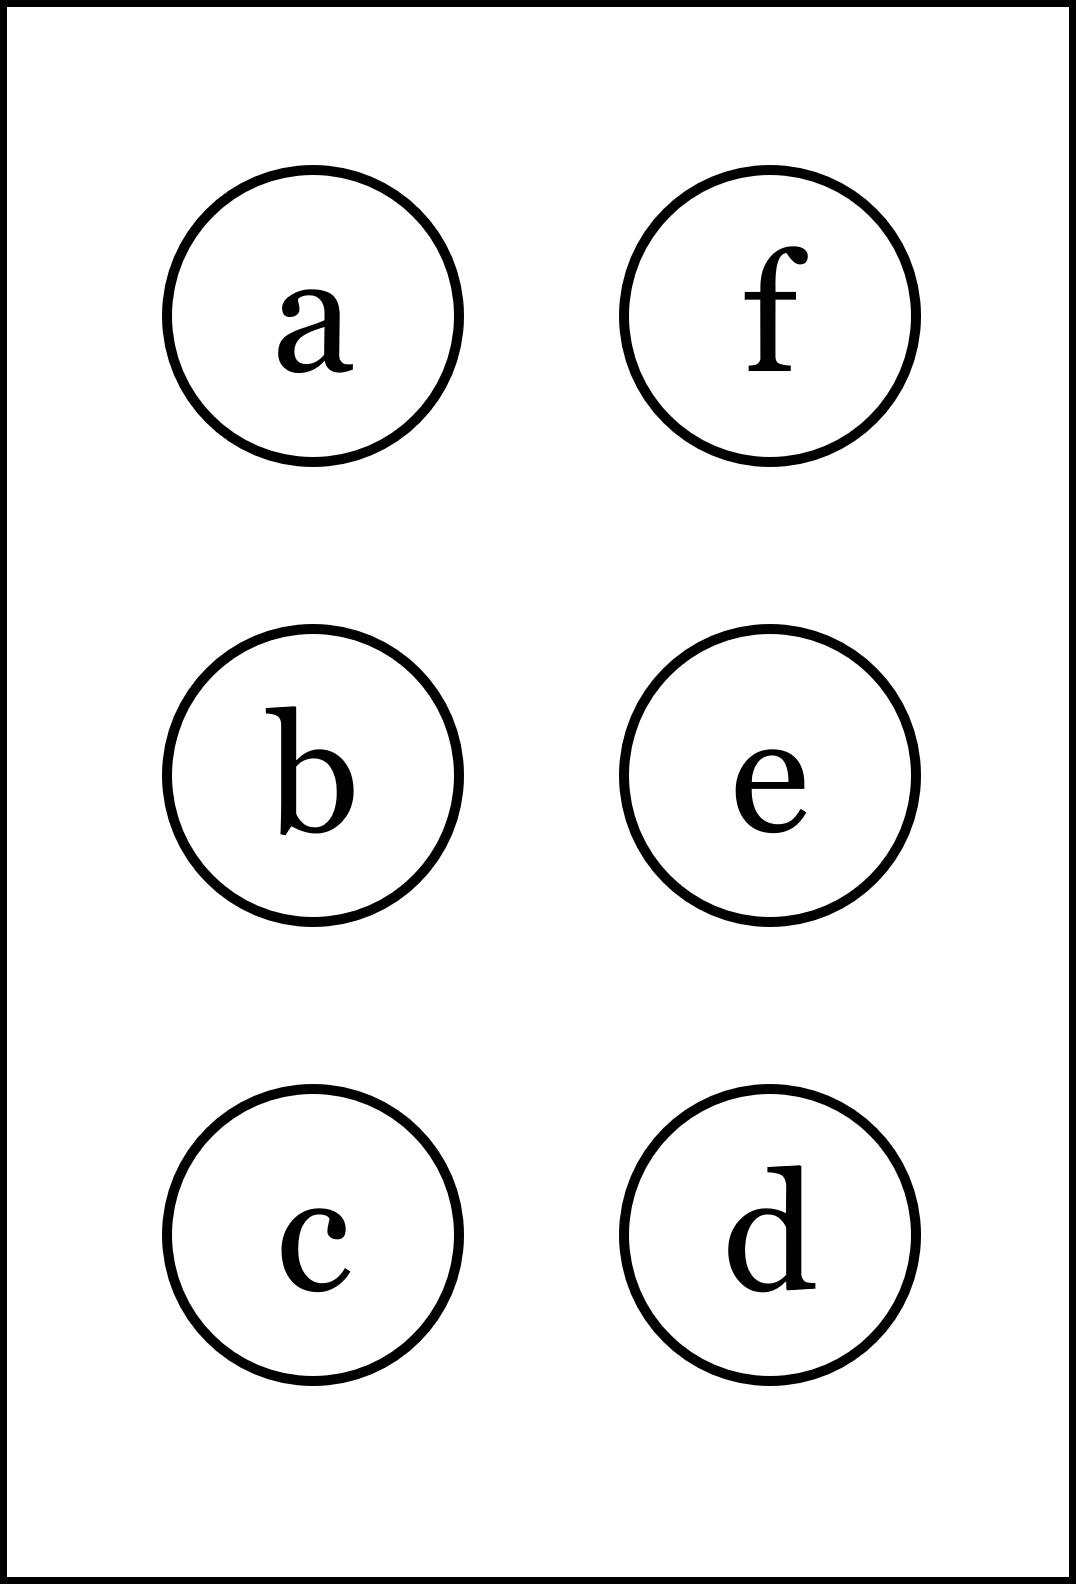
\includegraphics[height=40mm]{../images/braille.png}
{\small Písmeno Braillovej abecedy}
\end{center}
\end{minipage}
\end{center}
\end{minipage}
&
\begin{minipage}[c][104.5mm][t]{0.5\linewidth}
\begin{center}
\vspace{7mm}
{\huge Definiční obor, skupina \textit{Zeta $\zeta$} -\romannumeral4}\\[5mm]
\textit{Jméno:}\phantom{xxxxxxxxxxxxxxxxxxxxxxxxxxxxxxxxxxxxxxxxxxxxxxxxxxxxxxxxxxxxxxxxx}\\[5mm]
\begin{minipage}{0.95\linewidth}
\begin{center}
\textbf{Zjisti definiční obor} zadaných funkcí. Pokud se shoduje s tím za otazníky,\\tak napravo obarvi příslušející kroužek načerno. \textbf{Spolu odevzdejte výsledné slovo}.
\end{center}
\end{minipage}
\\[1mm]
\begin{minipage}{0.79\linewidth}
\begin{center}
\begin{varwidth}{\linewidth}
\begin{enumerate}
\normalsizerrr
\item $f(x)=\cfrac{-4x+1}{2x-6}$\quad \dotfill\; ???\;\dotfill \quad $\mathbb{R}\smallsetminus\{3\}$
\item $f(x)=\cfrac{1}{x^3-9x^2+15x-7}$\quad \dotfill\; ???\;\dotfill \quad $\mathbb{R}\smallsetminus\{1,2,-7\}$
\item $f(x)=-\sqrt{-7x+2}$\quad \dotfill\; ???\;\dotfill \quad $x\geq\nicefrac{2}{7}$
\item $f(x)=\sqrt{-x^2-x}$\quad \dotfill\; ???\;\dotfill \quad $x\in(-1 , 0)$
\item $f(x)=-4\ln{(-2x+4)}$\quad \dotfill\; ???\;\dotfill \quad $x<2$
\item $f(x)=\ln{(x^2+6x+8)}$\quad \dotfill\; ???\;\dotfill \quad $x\in(-\infty , -4)\cup(-2 , \infty)$
\end{enumerate}
\end{varwidth}
\end{center}
\end{minipage}
\begin{minipage}{0.20\linewidth}
\begin{center}
{\Huge\bfseries 4.} \\[2mm]
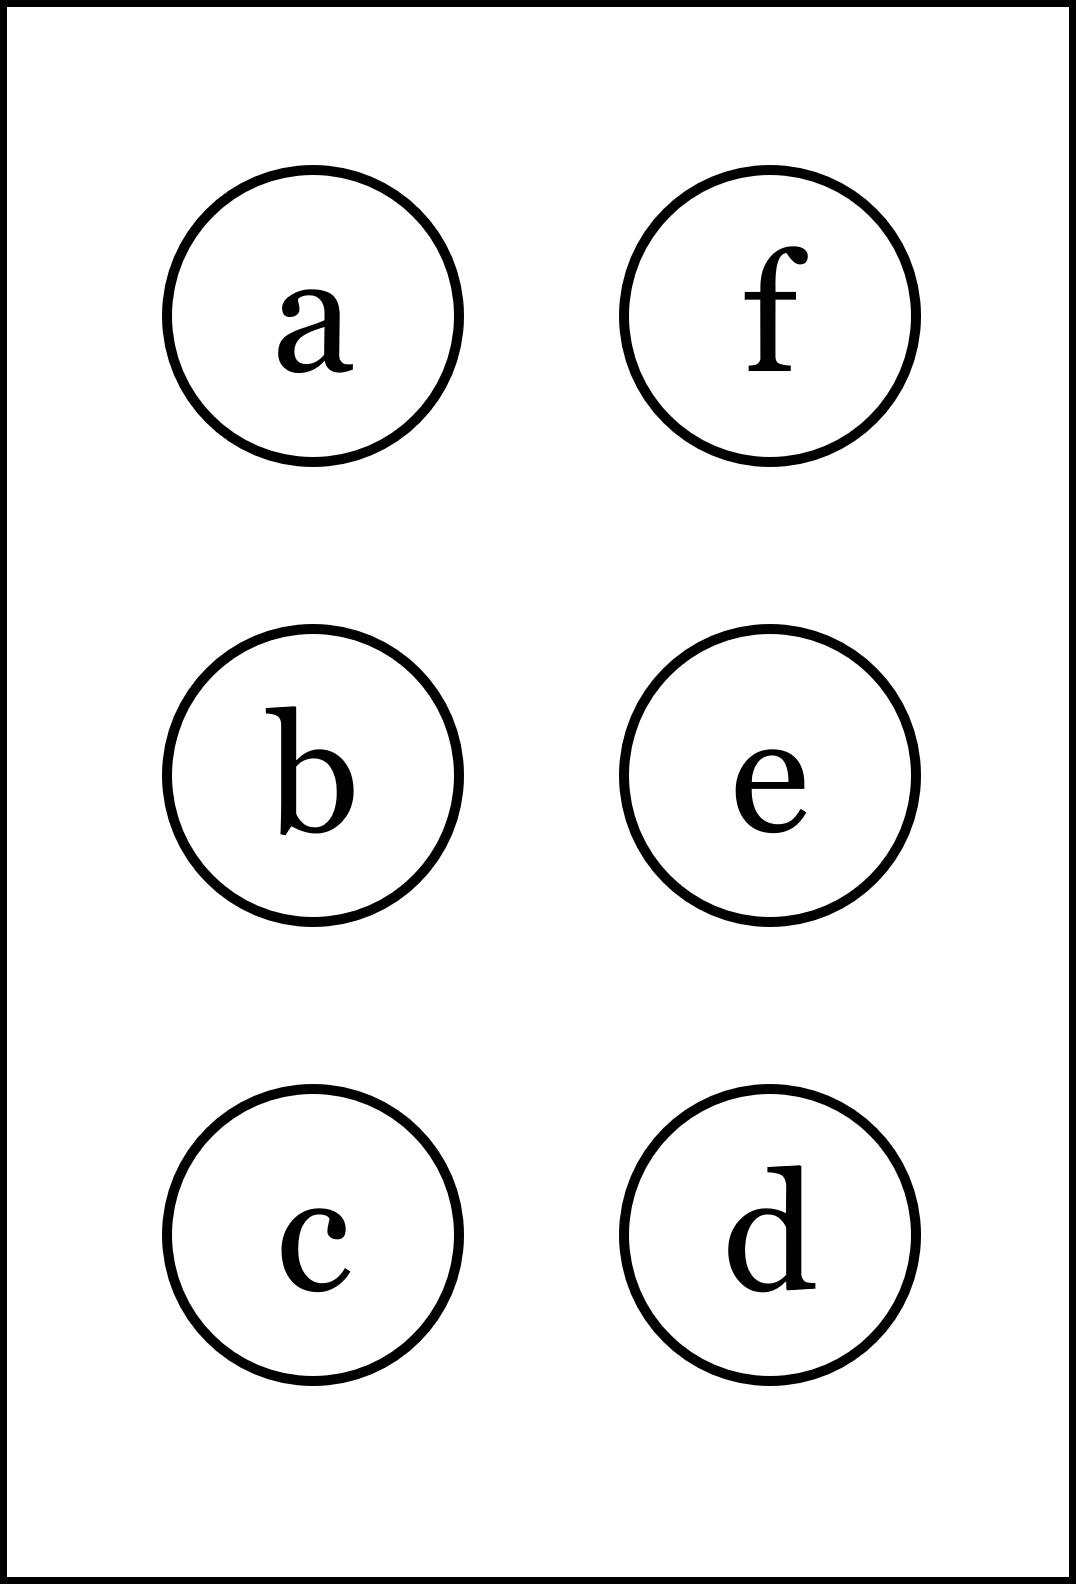
\includegraphics[height=40mm]{../images/braille.png}
{\small Písmeno Braillovej abecedy}
\end{center}
\end{minipage}
\end{center}
\end{minipage}
%
\end{tabular}
\newpage
\thispagestyle{empty}
\begin{tabular}{c:c}
\begin{minipage}[c][104.5mm][t]{0.5\linewidth}
\begin{center}
\vspace{7mm}
{\huge Definiční obor, skupina \textit{Eta $\eta$} -\romannumeral1}\\[5mm]
\textit{Jméno:}\phantom{xxxxxxxxxxxxxxxxxxxxxxxxxxxxxxxxxxxxxxxxxxxxxxxxxxxxxxxxxxxxxxxxx}\\[5mm]
\begin{minipage}{0.95\linewidth}
\begin{center}
\textbf{Zjisti definiční obor} zadaných funkcí. Pokud se shoduje s tím za otazníky,\\tak napravo obarvi příslušející kroužek načerno. \textbf{Spolu odevzdejte výsledné slovo}.
\end{center}
\end{minipage}
\\[1mm]
\begin{minipage}{0.79\linewidth}
\begin{center}
\begin{varwidth}{\linewidth}
\begin{enumerate}
\normalsizerrr
\item $f(x)=\cfrac{4x-3}{4x-3}$\quad \dotfill\; ???\;\dotfill \quad $\mathbb{R}\smallsetminus\{\nicefrac{-3}{4}\}$
\item $f(x)=\cfrac{1}{-2x^3-12x^2-10x+24}$\quad \dotfill\; ???\;\dotfill \quad $\mathbb{R}\smallsetminus\{1,-4,-3\}$
\item $f(x)=5\sqrt{-6x+9}$\quad \dotfill\; ???\;\dotfill \quad $x\leq\nicefrac{-3}{2}$
\item $f(x)=\sqrt{-x^2-5x}$\quad \dotfill\; ???\;\dotfill \quad $x\in\langle0 , 5\rangle$
\item $f(x)=-5\ln{(7x+6)}$\quad \dotfill\; ???\;\dotfill \quad $x>\nicefrac{6}{7}$
\item $f(x)=\ln{(x^2+x-30)}$\quad \dotfill\; ???\;\dotfill \quad $x\in(-\infty , -6)\cup(5 , \infty)$
\end{enumerate}
\end{varwidth}
\end{center}
\end{minipage}
\begin{minipage}{0.20\linewidth}
\begin{center}
{\Huge\bfseries 1.} \\[2mm]
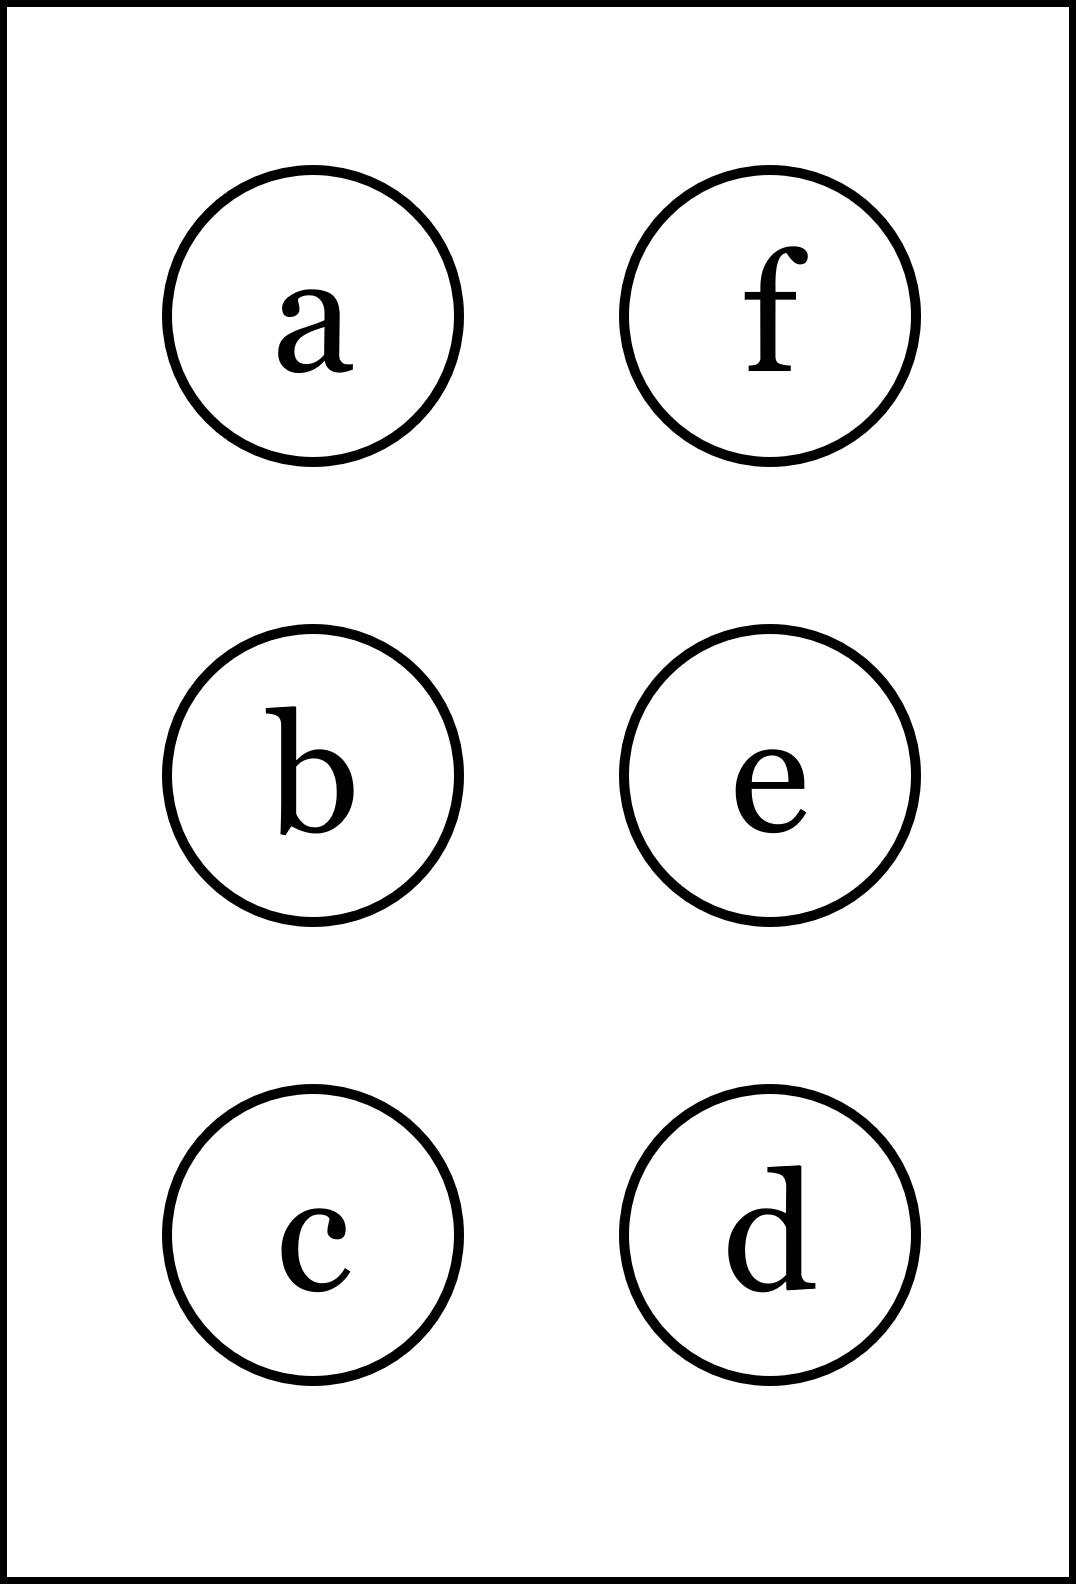
\includegraphics[height=40mm]{../images/braille.png}
{\small Písmeno Braillovej abecedy}
\end{center}
\end{minipage}
\end{center}
\end{minipage}
&
\begin{minipage}[c][104.5mm][t]{0.5\linewidth}
\begin{center}
\vspace{7mm}
{\huge Definiční obor, skupina \textit{Eta $\eta$} -\romannumeral2}\\[5mm]
\textit{Jméno:}\phantom{xxxxxxxxxxxxxxxxxxxxxxxxxxxxxxxxxxxxxxxxxxxxxxxxxxxxxxxxxxxxxxxxx}\\[5mm]
\begin{minipage}{0.95\linewidth}
\begin{center}
\textbf{Zjisti definiční obor} zadaných funkcí. Pokud se shoduje s tím za otazníky,\\tak napravo obarvi příslušející kroužek načerno. \textbf{Spolu odevzdejte výsledné slovo}.
\end{center}
\end{minipage}
\\[1mm]
\begin{minipage}{0.79\linewidth}
\begin{center}
\begin{varwidth}{\linewidth}
\begin{enumerate}
\normalsizerrr
\item $f(x)=\cfrac{-4x+1}{-x-5}$\quad \dotfill\; ???\;\dotfill \quad $\mathbb{R}\smallsetminus\{-5\}$
\item $f(x)=\cfrac{1}{-x^3-3x^2+10x+24}$\quad \dotfill\; ???\;\dotfill \quad $\mathbb{R}\smallsetminus\{3,-4,-2\}$
\item $f(x)=4\sqrt{8x-4}$\quad \dotfill\; ???\;\dotfill \quad $x\leq\nicefrac{1}{2}$
\item $f(x)=\sqrt{-x^2-6x}$\quad \dotfill\; ???\;\dotfill \quad $x\in\langle0 , 6\rangle$
\item $f(x)=\ln{(5x+8)}$\quad \dotfill\; ???\;\dotfill \quad $x>\nicefrac{-8}{5}$
\item $f(x)=\ln{(x^2+11x+24)}$\quad \dotfill\; ???\;\dotfill \quad $x\in(-\infty , -8)\cup(-3 , \infty)$
\end{enumerate}
\end{varwidth}
\end{center}
\end{minipage}
\begin{minipage}{0.20\linewidth}
\begin{center}
{\Huge\bfseries 2.} \\[2mm]
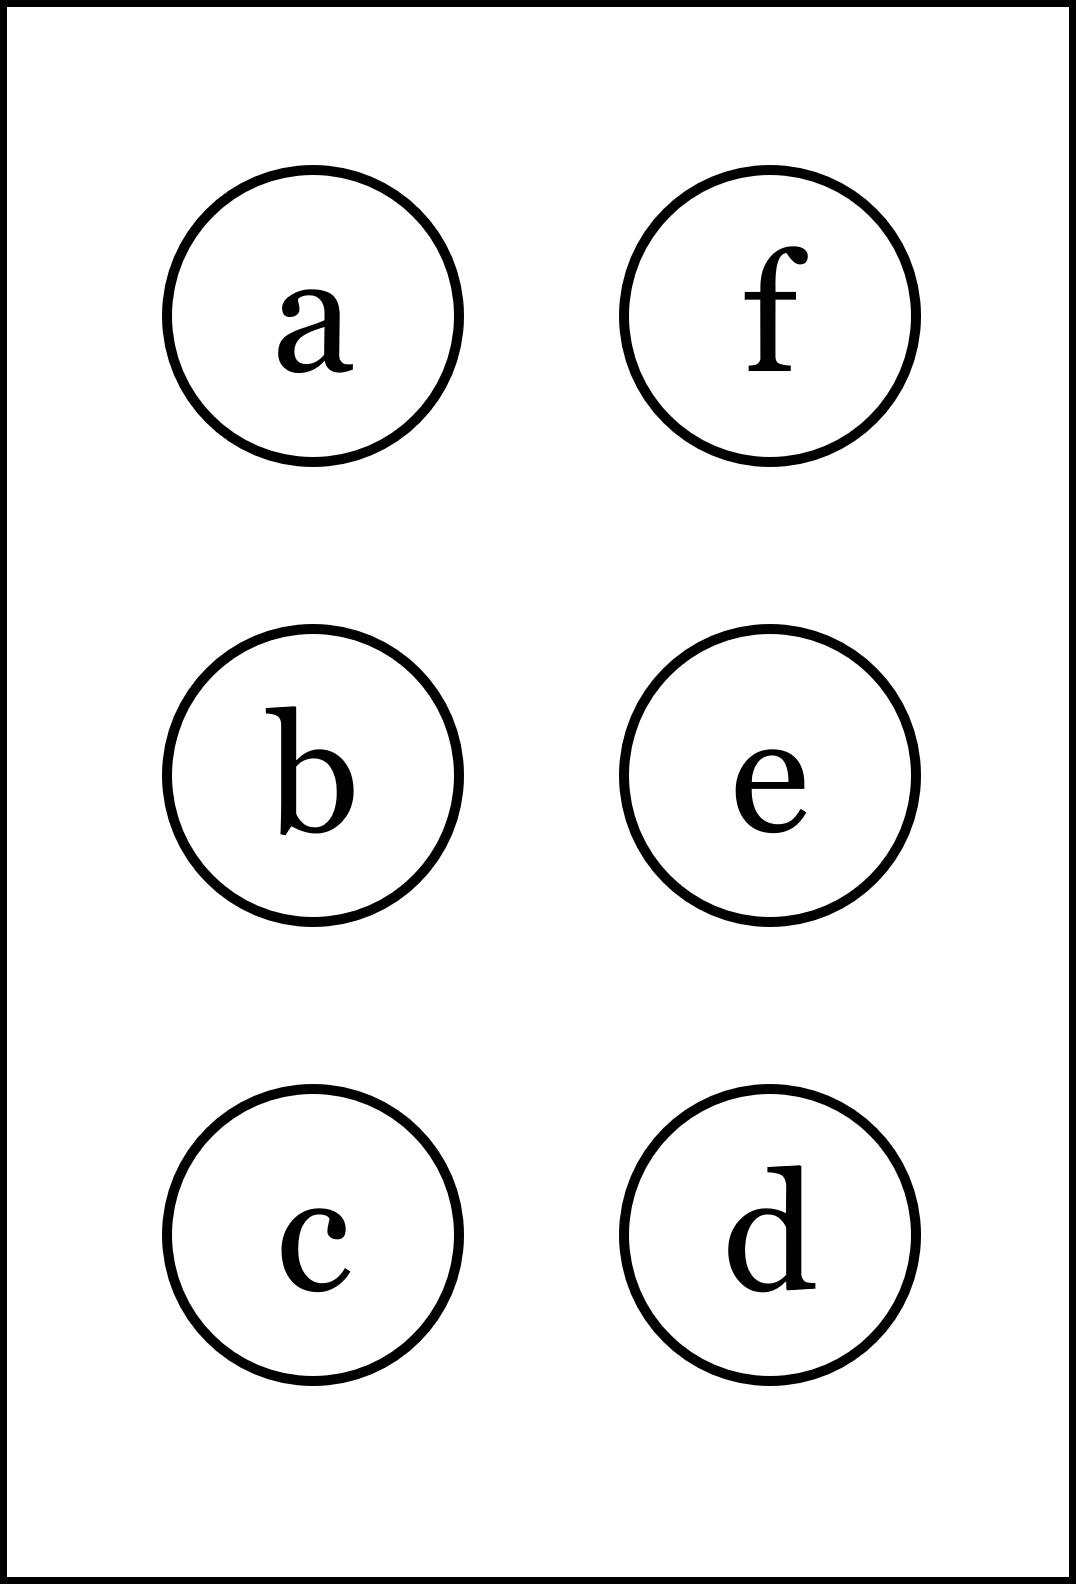
\includegraphics[height=40mm]{../images/braille.png}
{\small Písmeno Braillovej abecedy}
\end{center}
\end{minipage}
\end{center}
\end{minipage}
\\ \hdashline
\begin{minipage}[c][104.5mm][t]{0.5\linewidth}
\begin{center}
\vspace{7mm}
{\huge Definiční obor, skupina \textit{Eta $\eta$} -\romannumeral3}\\[5mm]
\textit{Jméno:}\phantom{xxxxxxxxxxxxxxxxxxxxxxxxxxxxxxxxxxxxxxxxxxxxxxxxxxxxxxxxxxxxxxxxx}\\[5mm]
\begin{minipage}{0.95\linewidth}
\begin{center}
\textbf{Zjisti definiční obor} zadaných funkcí. Pokud se shoduje s tím za otazníky,\\tak napravo obarvi příslušející kroužek načerno. \textbf{Spolu odevzdejte výsledné slovo}.
\end{center}
\end{minipage}
\\[1mm]
\begin{minipage}{0.79\linewidth}
\begin{center}
\begin{varwidth}{\linewidth}
\begin{enumerate}
\normalsizerrr
\item $f(x)=\cfrac{-4x+1}{4x+6}$\quad \dotfill\; ???\;\dotfill \quad $\mathbb{R}\smallsetminus\{\nicefrac{-3}{2}\}$
\item $f(x)=\cfrac{1}{3x^3-12x^2-21x+30}$\quad \dotfill\; ???\;\dotfill \quad $\mathbb{R}\smallsetminus\{1,5,-2\}$
\item $f(x)=-2\sqrt{-8x-5}$\quad \dotfill\; ???\;\dotfill \quad $x\leq\nicefrac{-5}{8}$
\item $f(x)=\sqrt{-x^2-5x}$\quad \dotfill\; ???\;\dotfill \quad $x\in(-5 , 0)$
\item $f(x)=-2\ln{(-6x-1)}$\quad \dotfill\; ???\;\dotfill \quad $x>\nicefrac{-1}{6}$
\item $f(x)=\ln{(x^2-x-6)}$\quad \dotfill\; ???\;\dotfill \quad $x\in(-2 , 3)$
\end{enumerate}
\end{varwidth}
\end{center}
\end{minipage}
\begin{minipage}{0.20\linewidth}
\begin{center}
{\Huge\bfseries 3.} \\[2mm]
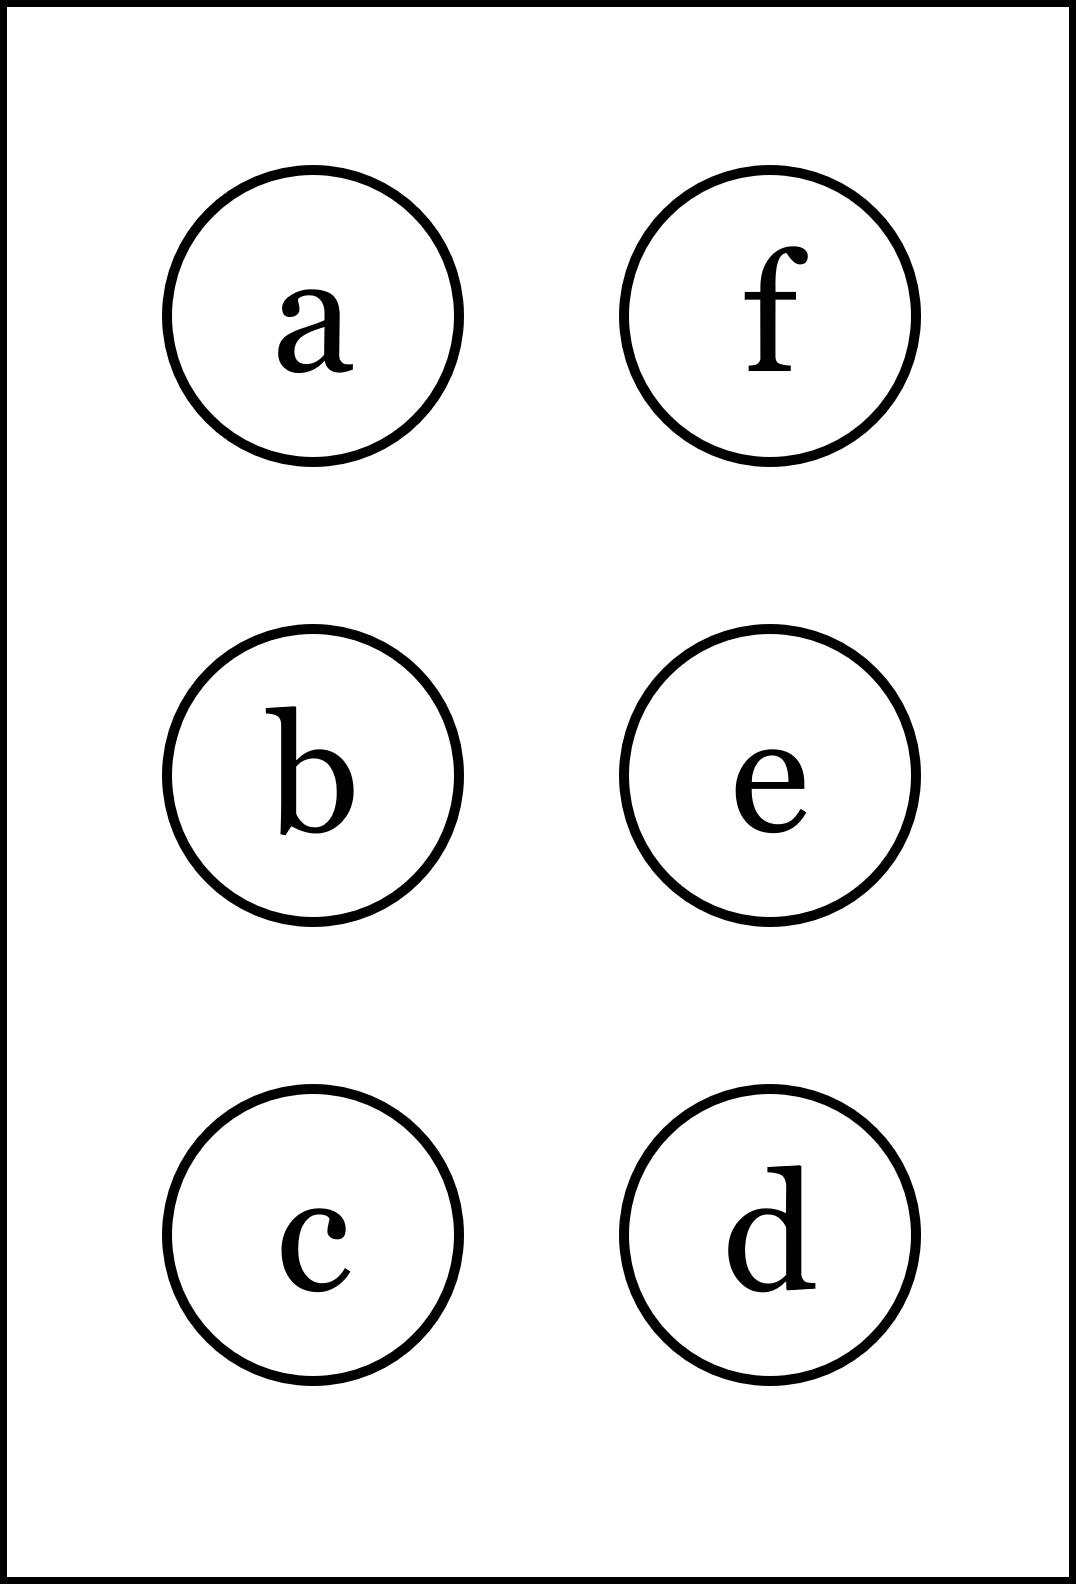
\includegraphics[height=40mm]{../images/braille.png}
{\small Písmeno Braillovej abecedy}
\end{center}
\end{minipage}
\end{center}
\end{minipage}
&
\begin{minipage}[c][104.5mm][t]{0.5\linewidth}
\begin{center}
\vspace{7mm}
{\huge Definiční obor, skupina \textit{Eta $\eta$} -\romannumeral4}\\[5mm]
\textit{Jméno:}\phantom{xxxxxxxxxxxxxxxxxxxxxxxxxxxxxxxxxxxxxxxxxxxxxxxxxxxxxxxxxxxxxxxxx}\\[5mm]
\begin{minipage}{0.95\linewidth}
\begin{center}
\textbf{Zjisti definiční obor} zadaných funkcí. Pokud se shoduje s tím za otazníky,\\tak napravo obarvi příslušející kroužek načerno. \textbf{Spolu odevzdejte výsledné slovo}.
\end{center}
\end{minipage}
\\[1mm]
\begin{minipage}{0.79\linewidth}
\begin{center}
\begin{varwidth}{\linewidth}
\begin{enumerate}
\normalsizerrr
\item $f(x)=\cfrac{2x-1}{8x-1}$\quad \dotfill\; ???\;\dotfill \quad $\mathbb{R}\smallsetminus\{\nicefrac{1}{8}\}$
\item $f(x)=\cfrac{1}{-2x^3-10x^2-4x+16}$\quad \dotfill\; ???\;\dotfill \quad $\mathbb{R}\smallsetminus\{-6,-2,-1\}$
\item $f(x)=5\sqrt{x+4}$\quad \dotfill\; ???\;\dotfill \quad $x\geq-4$
\item $f(x)=\sqrt{-x^2-5x}$\quad \dotfill\; ???\;\dotfill \quad $x\in\langle-5 , 0\rangle$
\item $f(x)=-2\ln{(3x+2)}$\quad \dotfill\; ???\;\dotfill \quad $x>\nicefrac{2}{3}$
\item $f(x)=\ln{(x^2+12x+35)}$\quad \dotfill\; ???\;\dotfill \quad $x\in(-7 , -5)$
\end{enumerate}
\end{varwidth}
\end{center}
\end{minipage}
\begin{minipage}{0.20\linewidth}
\begin{center}
{\Huge\bfseries 4.} \\[2mm]
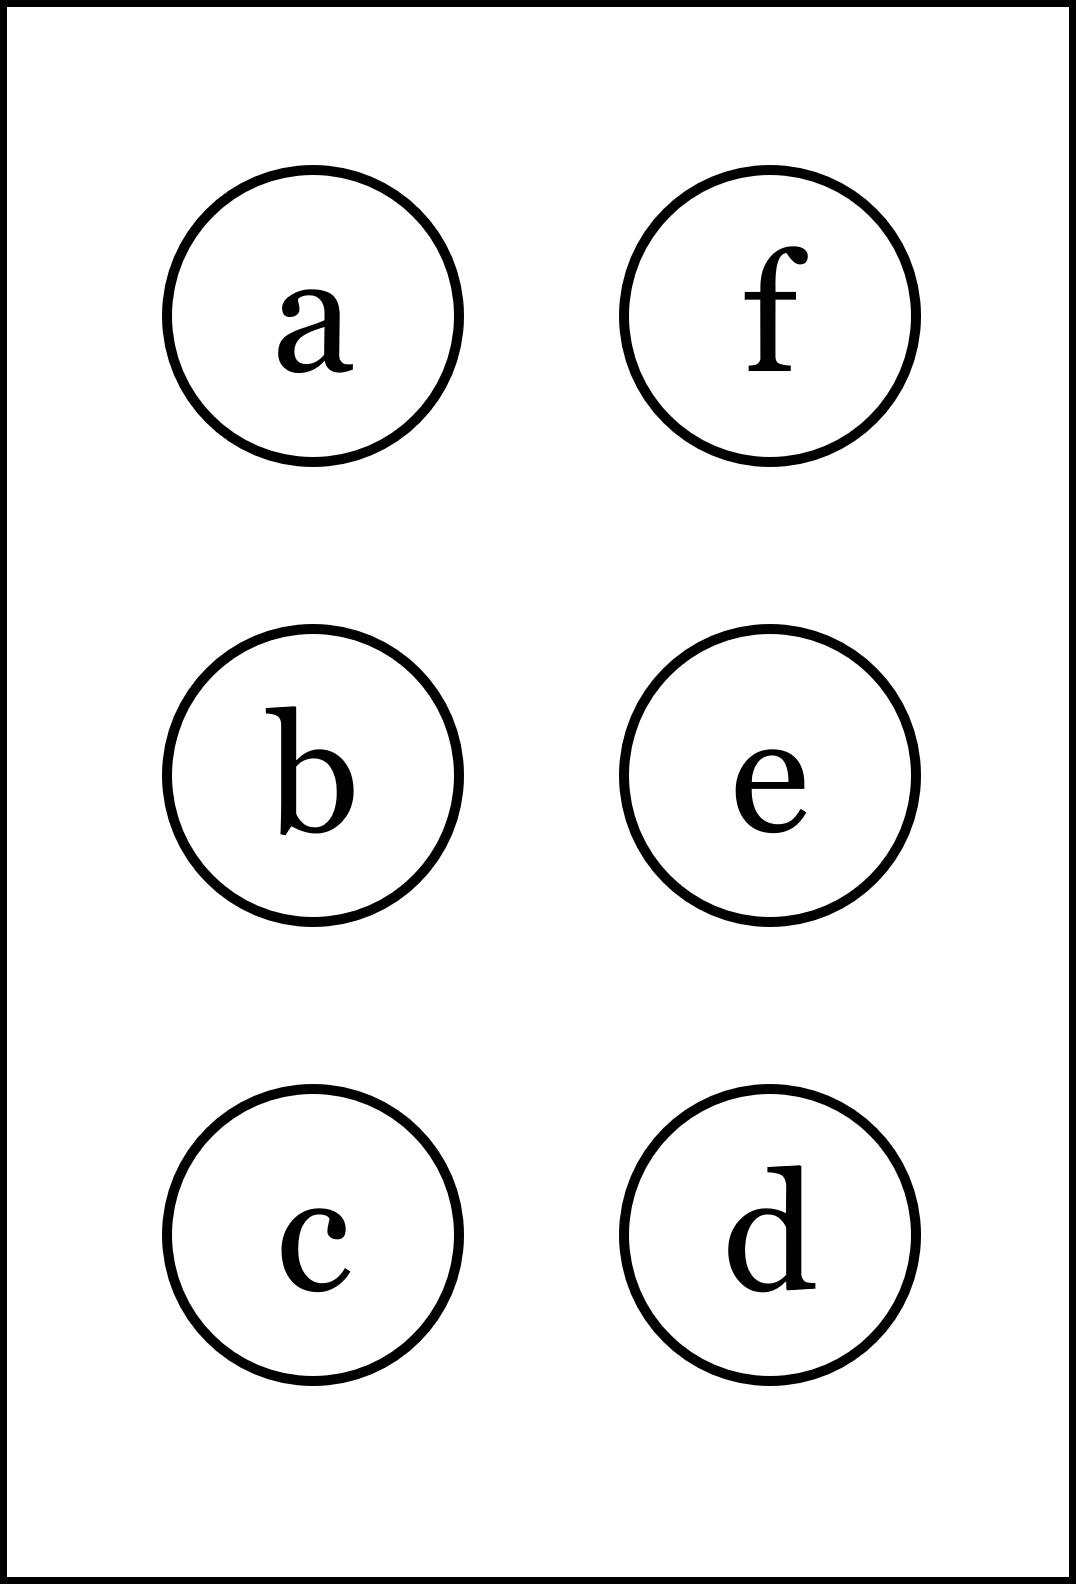
\includegraphics[height=40mm]{../images/braille.png}
{\small Písmeno Braillovej abecedy}
\end{center}
\end{minipage}
\end{center}
\end{minipage}
%
\end{tabular}
\newpage
\thispagestyle{empty}
\begin{tabular}{c:c}
\begin{minipage}[c][104.5mm][t]{0.5\linewidth}
\begin{center}
\vspace{7mm}
{\huge Definiční obor, skupina \textit{Theta $\theta$} -\romannumeral1}\\[5mm]
\textit{Jméno:}\phantom{xxxxxxxxxxxxxxxxxxxxxxxxxxxxxxxxxxxxxxxxxxxxxxxxxxxxxxxxxxxxxxxxx}\\[5mm]
\begin{minipage}{0.95\linewidth}
\begin{center}
\textbf{Zjisti definiční obor} zadaných funkcí. Pokud se shoduje s tím za otazníky,\\tak napravo obarvi příslušející kroužek načerno. \textbf{Spolu odevzdejte výsledné slovo}.
\end{center}
\end{minipage}
\\[1mm]
\begin{minipage}{0.79\linewidth}
\begin{center}
\begin{varwidth}{\linewidth}
\begin{enumerate}
\normalsizerrr
\item $f(x)=\cfrac{5x-5}{-3x+6}$\quad \dotfill\; ???\;\dotfill \quad $\mathbb{R}\smallsetminus\{2\}$
\item $f(x)=\cfrac{1}{x^3-8x^2+17x-10}$\quad \dotfill\; ???\;\dotfill \quad $\mathbb{R}\smallsetminus\{1,4,-2\}$
\item $f(x)=5\sqrt{-6x+4}$\quad \dotfill\; ???\;\dotfill \quad $x\leq\nicefrac{2}{3}$
\item $f(x)=\sqrt{-x^2-6x}$\quad \dotfill\; ???\;\dotfill \quad $x\in\langle-6 , 0\rangle$
\item $f(x)=2\ln{(-5x-5)}$\quad \dotfill\; ???\;\dotfill \quad $x<1$
\item $f(x)=\ln{(x^2-8x+12)}$\quad \dotfill\; ???\;\dotfill \quad $x\in(2 , 6)$
\end{enumerate}
\end{varwidth}
\end{center}
\end{minipage}
\begin{minipage}{0.20\linewidth}
\begin{center}
{\Huge\bfseries 1.} \\[2mm]
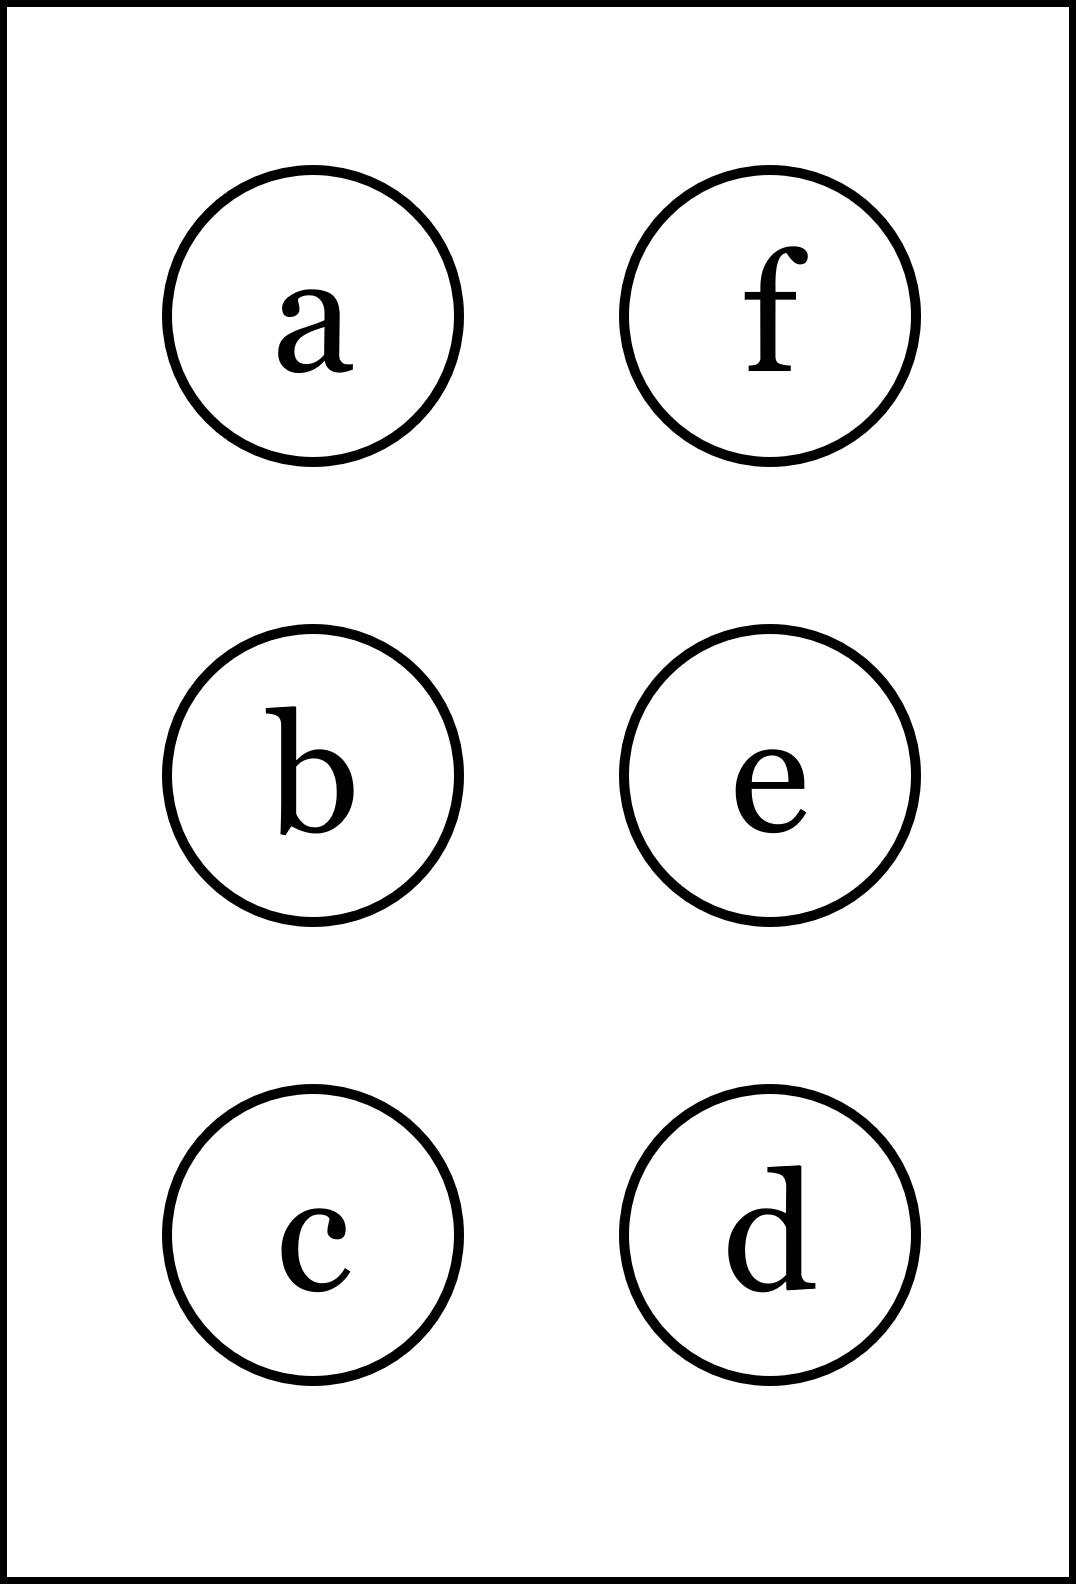
\includegraphics[height=40mm]{../images/braille.png}
{\small Písmeno Braillovej abecedy}
\end{center}
\end{minipage}
\end{center}
\end{minipage}
&
\begin{minipage}[c][104.5mm][t]{0.5\linewidth}
\begin{center}
\vspace{7mm}
{\huge Definiční obor, skupina \textit{Theta $\theta$} -\romannumeral2}\\[5mm]
\textit{Jméno:}\phantom{xxxxxxxxxxxxxxxxxxxxxxxxxxxxxxxxxxxxxxxxxxxxxxxxxxxxxxxxxxxxxxxxx}\\[5mm]
\begin{minipage}{0.95\linewidth}
\begin{center}
\textbf{Zjisti definiční obor} zadaných funkcí. Pokud se shoduje s tím za otazníky,\\tak napravo obarvi příslušející kroužek načerno. \textbf{Spolu odevzdejte výsledné slovo}.
\end{center}
\end{minipage}
\\[1mm]
\begin{minipage}{0.79\linewidth}
\begin{center}
\begin{varwidth}{\linewidth}
\begin{enumerate}
\normalsizerrr
\item $f(x)=\cfrac{4x+3}{6x+6}$\quad \dotfill\; ???\;\dotfill \quad $\mathbb{R}\smallsetminus\{-1\}$
\item $f(x)=\cfrac{1}{-x^3-9x^2-23x-15}$\quad \dotfill\; ???\;\dotfill \quad $\mathbb{R}\smallsetminus\{5,-3\}$
\item $f(x)=-\sqrt{4x+5}$\quad \dotfill\; ???\;\dotfill \quad $x\leq\nicefrac{-5}{4}$
\item $f(x)=\sqrt{-x^2-x}$\quad \dotfill\; ???\;\dotfill \quad $x\in\langle0 , 1\rangle$
\item $f(x)=2\ln{(-x-4)}$\quad \dotfill\; ???\;\dotfill \quad $x<4$
\item $f(x)=\ln{(x^2+3x-4)}$\quad \dotfill\; ???\;\dotfill \quad $x\in(-\infty , -4)\cup(1 , \infty)$
\end{enumerate}
\end{varwidth}
\end{center}
\end{minipage}
\begin{minipage}{0.20\linewidth}
\begin{center}
{\Huge\bfseries 2.} \\[2mm]
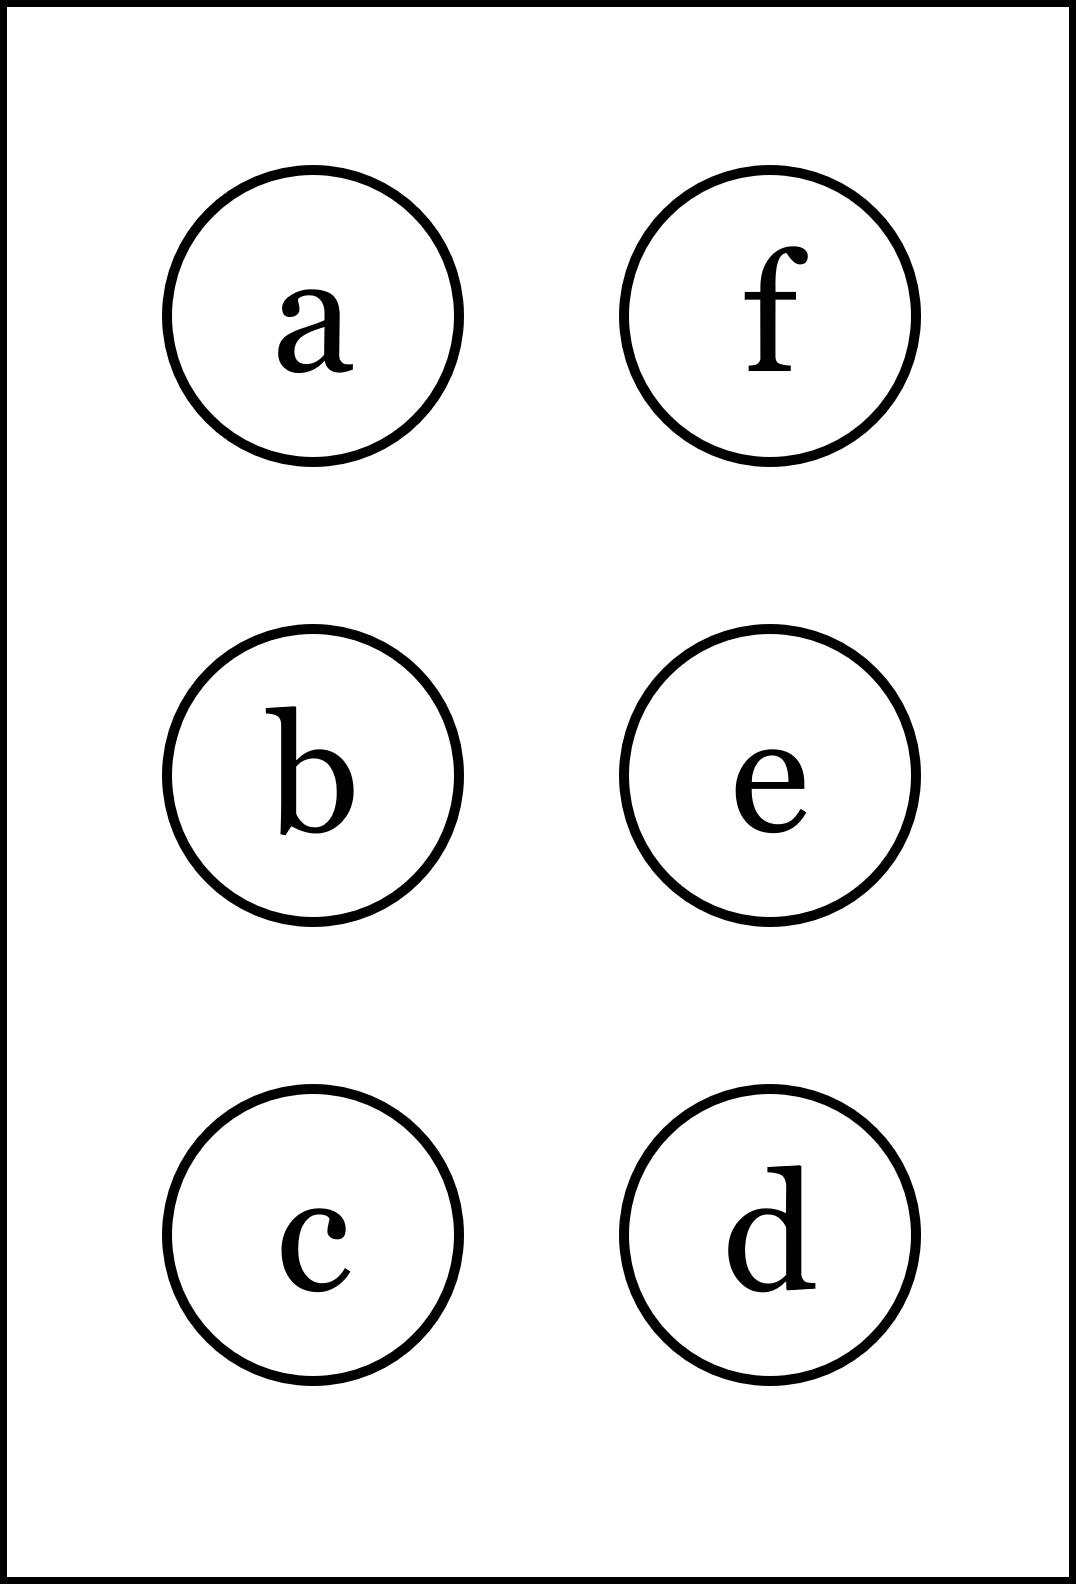
\includegraphics[height=40mm]{../images/braille.png}
{\small Písmeno Braillovej abecedy}
\end{center}
\end{minipage}
\end{center}
\end{minipage}
\\ \hdashline
\begin{minipage}[c][104.5mm][t]{0.5\linewidth}
\begin{center}
\vspace{7mm}
{\huge Definiční obor, skupina \textit{Theta $\theta$} -\romannumeral3}\\[5mm]
\textit{Jméno:}\phantom{xxxxxxxxxxxxxxxxxxxxxxxxxxxxxxxxxxxxxxxxxxxxxxxxxxxxxxxxxxxxxxxxx}\\[5mm]
\begin{minipage}{0.95\linewidth}
\begin{center}
\textbf{Zjisti definiční obor} zadaných funkcí. Pokud se shoduje s tím za otazníky,\\tak napravo obarvi příslušející kroužek načerno. \textbf{Spolu odevzdejte výsledné slovo}.
\end{center}
\end{minipage}
\\[1mm]
\begin{minipage}{0.79\linewidth}
\begin{center}
\begin{varwidth}{\linewidth}
\begin{enumerate}
\normalsizerrr
\item $f(x)=\cfrac{-x-1}{4x-4}$\quad \dotfill\; ???\;\dotfill \quad $\mathbb{R}\smallsetminus\{1\}$
\item $f(x)=\cfrac{1}{3x^3+27x^2+18x-48}$\quad \dotfill\; ???\;\dotfill \quad $\mathbb{R}\smallsetminus\{-8,1,-2\}$
\item $f(x)=-2\sqrt{5x-3}$\quad \dotfill\; ???\;\dotfill \quad $x\leq\nicefrac{3}{5}$
\item $f(x)=\sqrt{-x^2+2x}$\quad \dotfill\; ???\;\dotfill \quad $x\in(0 , 2)$
\item $f(x)=-8\ln{(7x-5)}$\quad \dotfill\; ???\;\dotfill \quad $x>\nicefrac{5}{7}$
\item $f(x)=\ln{(x^2+2x-3)}$\quad \dotfill\; ???\;\dotfill \quad $x\in(-3 , 1)$
\end{enumerate}
\end{varwidth}
\end{center}
\end{minipage}
\begin{minipage}{0.20\linewidth}
\begin{center}
{\Huge\bfseries 3.} \\[2mm]
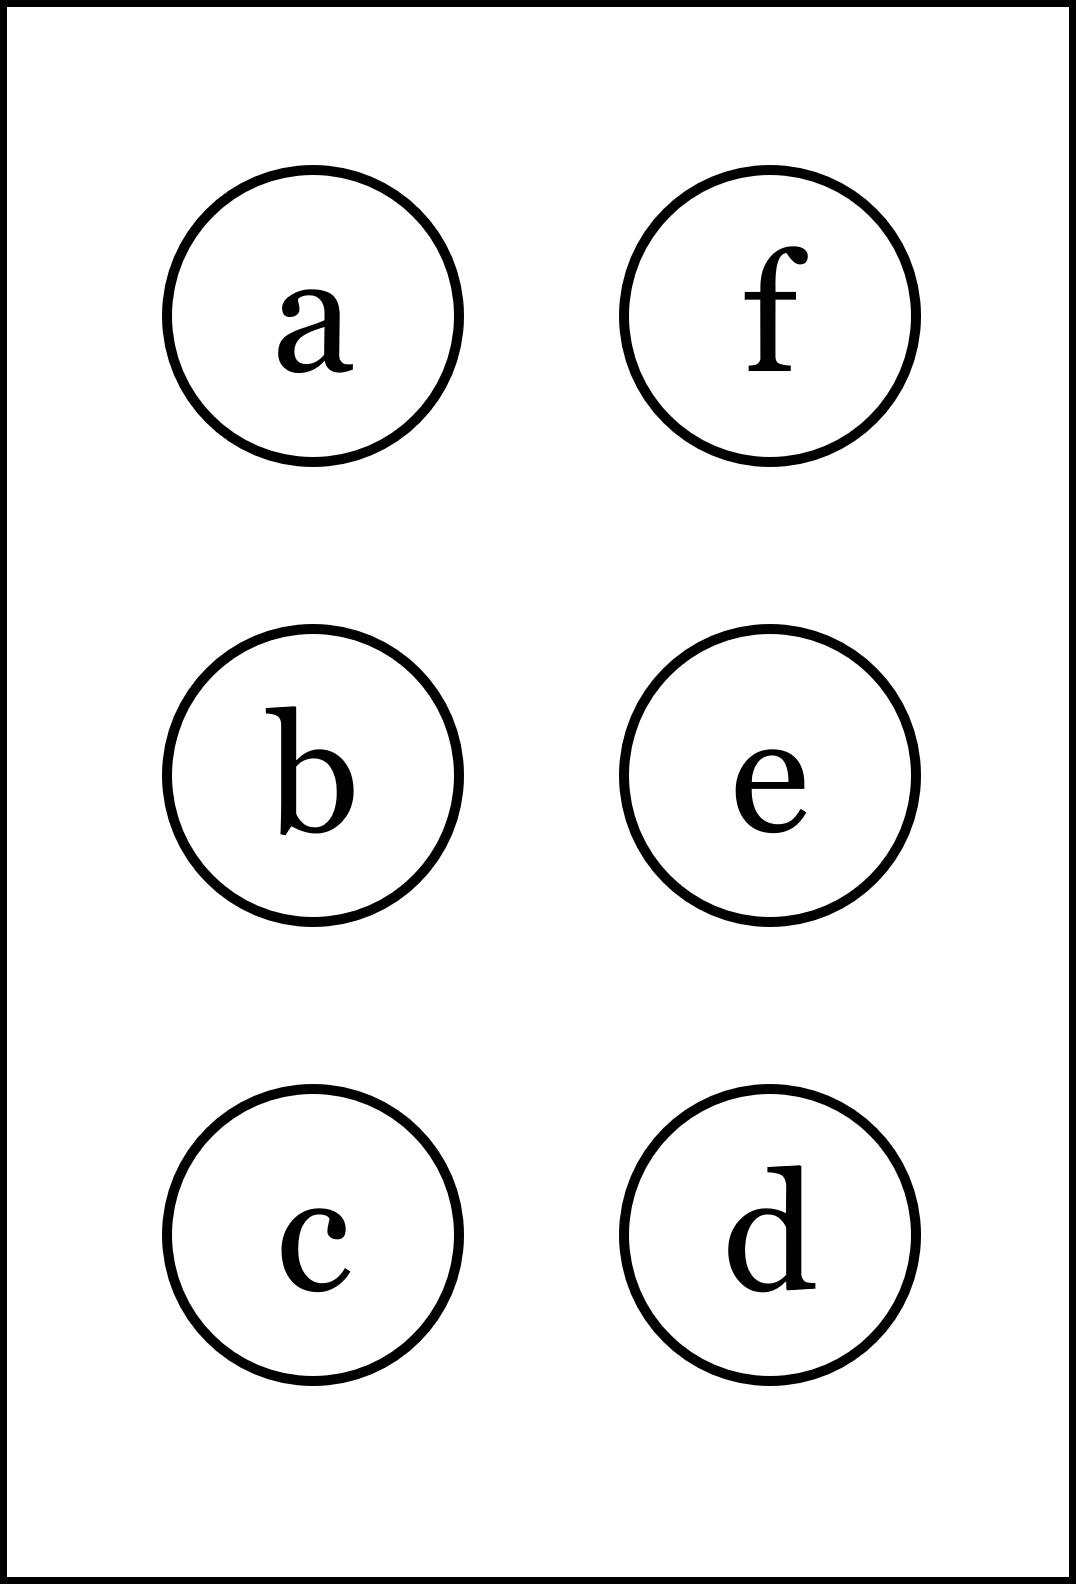
\includegraphics[height=40mm]{../images/braille.png}
{\small Písmeno Braillovej abecedy}
\end{center}
\end{minipage}
\end{center}
\end{minipage}
&
\begin{minipage}[c][104.5mm][t]{0.5\linewidth}
\begin{center}
\vspace{7mm}
{\huge Definiční obor, skupina \textit{Theta $\theta$} -\romannumeral4}\\[5mm]
\textit{Jméno:}\phantom{xxxxxxxxxxxxxxxxxxxxxxxxxxxxxxxxxxxxxxxxxxxxxxxxxxxxxxxxxxxxxxxxx}\\[5mm]
\begin{minipage}{0.95\linewidth}
\begin{center}
\textbf{Zjisti definiční obor} zadaných funkcí. Pokud se shoduje s tím za otazníky,\\tak napravo obarvi příslušející kroužek načerno. \textbf{Spolu odevzdejte výsledné slovo}.
\end{center}
\end{minipage}
\\[1mm]
\begin{minipage}{0.79\linewidth}
\begin{center}
\begin{varwidth}{\linewidth}
\begin{enumerate}
\normalsizerrr
\item $f(x)=\cfrac{7x-3}{-5x+1}$\quad \dotfill\; ???\;\dotfill \quad $\mathbb{R}\smallsetminus\{\nicefrac{1}{5}\}$
\item $f(x)=\cfrac{1}{-5x^3+10x^2+5x-10}$\quad \dotfill\; ???\;\dotfill \quad $\mathbb{R}\smallsetminus\{3,-1,-2\}$
\item $f(x)=\sqrt{2x-1}$\quad \dotfill\; ???\;\dotfill \quad $x\geq\nicefrac{1}{2}$
\item $f(x)=\sqrt{-x^2-5x}$\quad \dotfill\; ???\;\dotfill \quad $x\in(-5 , 0)$
\item $f(x)=6\ln{(8x+9)}$\quad \dotfill\; ???\;\dotfill \quad $x>\nicefrac{-9}{8}$
\item $f(x)=\ln{(x^2+8x+12)}$\quad \dotfill\; ???\;\dotfill \quad $x\in(-6 , -2)$
\end{enumerate}
\end{varwidth}
\end{center}
\end{minipage}
\begin{minipage}{0.20\linewidth}
\begin{center}
{\Huge\bfseries 4.} \\[2mm]
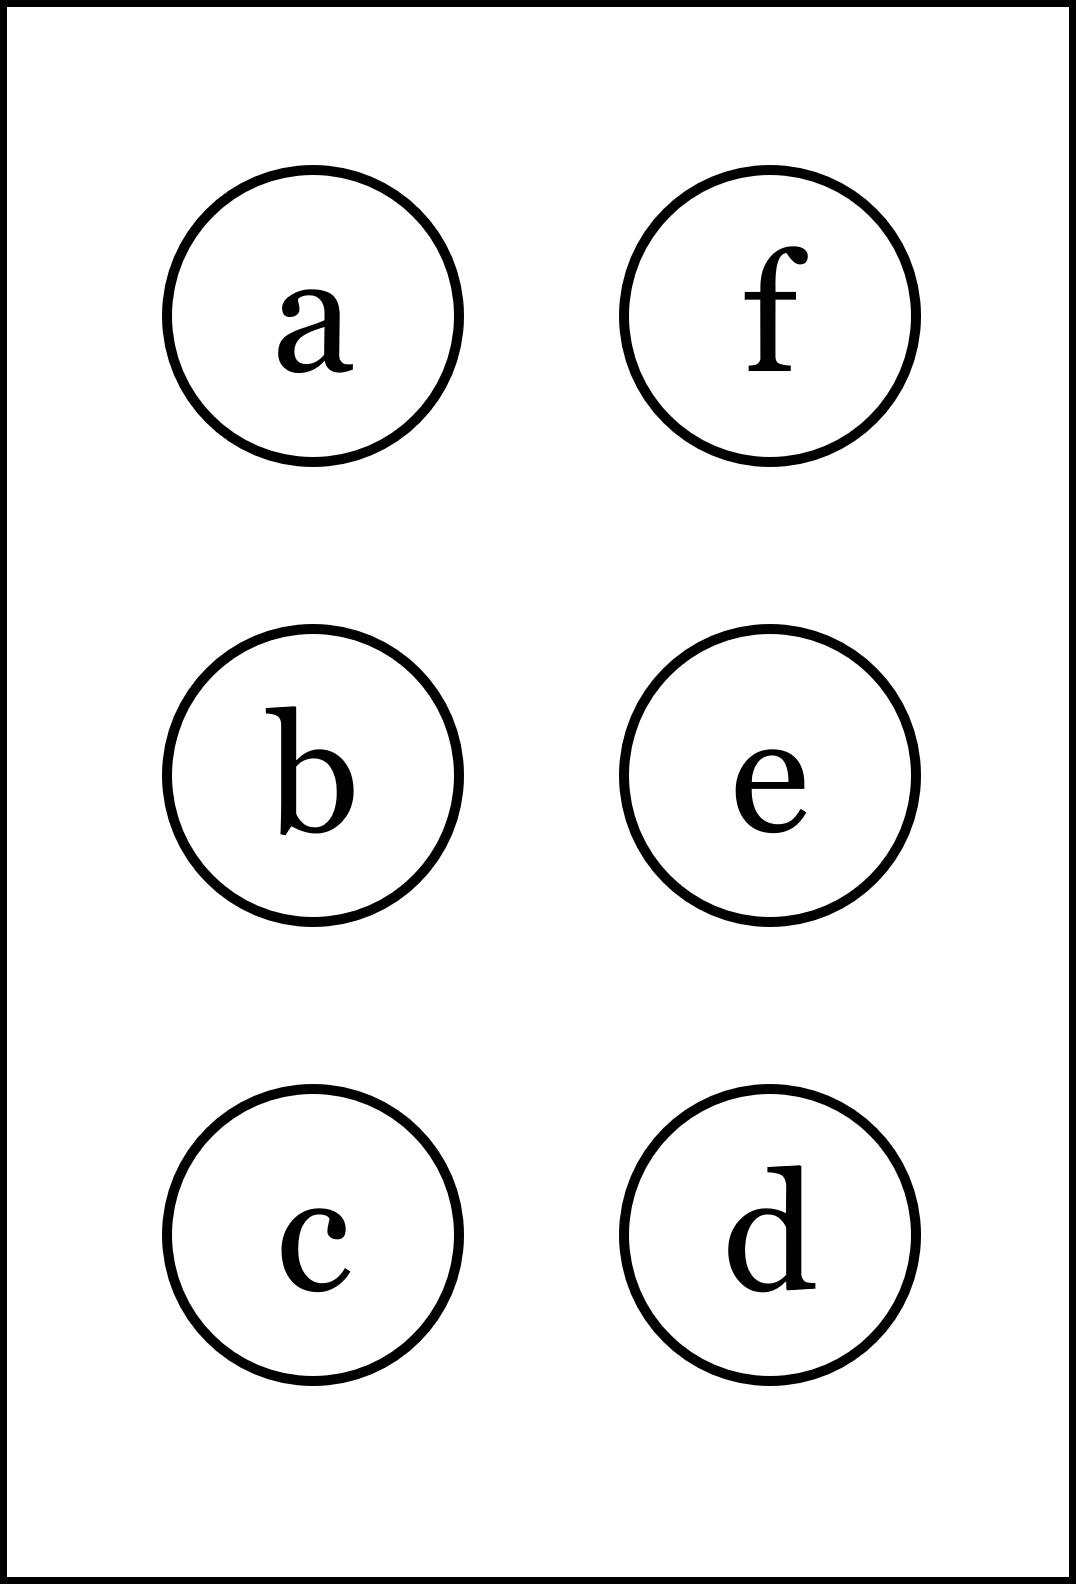
\includegraphics[height=40mm]{../images/braille.png}
{\small Písmeno Braillovej abecedy}
\end{center}
\end{minipage}
\end{center}
\end{minipage}
%
\end{tabular}
\newpage
\thispagestyle{empty}
\begin{tabular}{c:c}
\begin{minipage}[c][104.5mm][t]{0.5\linewidth}
\begin{center}
\vspace{7mm}
{\huge Definiční obor, skupina \textit{Iota $\iota$} -\romannumeral1}\\[5mm]
\textit{Jméno:}\phantom{xxxxxxxxxxxxxxxxxxxxxxxxxxxxxxxxxxxxxxxxxxxxxxxxxxxxxxxxxxxxxxxxx}\\[5mm]
\begin{minipage}{0.95\linewidth}
\begin{center}
\textbf{Zjisti definiční obor} zadaných funkcí. Pokud se shoduje s tím za otazníky,\\tak napravo obarvi příslušející kroužek načerno. \textbf{Spolu odevzdejte výsledné slovo}.
\end{center}
\end{minipage}
\\[1mm]
\begin{minipage}{0.79\linewidth}
\begin{center}
\begin{varwidth}{\linewidth}
\begin{enumerate}
\normalsizerrr
\item $f(x)=\cfrac{9x-3}{2x-5}$\quad \dotfill\; ???\;\dotfill \quad $\mathbb{R}\smallsetminus\{\nicefrac{5}{2}\}$
\item $f(x)=\cfrac{1}{-x^3+9x^2-15x-25}$\quad \dotfill\; ???\;\dotfill \quad $\mathbb{R}\smallsetminus\{-5,5,-2\}$
\item $f(x)=5\sqrt{2x-4}$\quad \dotfill\; ???\;\dotfill \quad $x\geq2$
\item $f(x)=\sqrt{-x^2+5x}$\quad \dotfill\; ???\;\dotfill \quad $x\in\langle0 , 5\rangle$
\item $f(x)=-5\ln{(3x+1)}$\quad \dotfill\; ???\;\dotfill \quad $x>\nicefrac{1}{3}$
\item $f(x)=\ln{(x^2+2x-15)}$\quad \dotfill\; ???\;\dotfill \quad $x\in(-5 , 3)$
\end{enumerate}
\end{varwidth}
\end{center}
\end{minipage}
\begin{minipage}{0.20\linewidth}
\begin{center}
{\Huge\bfseries 1.} \\[2mm]
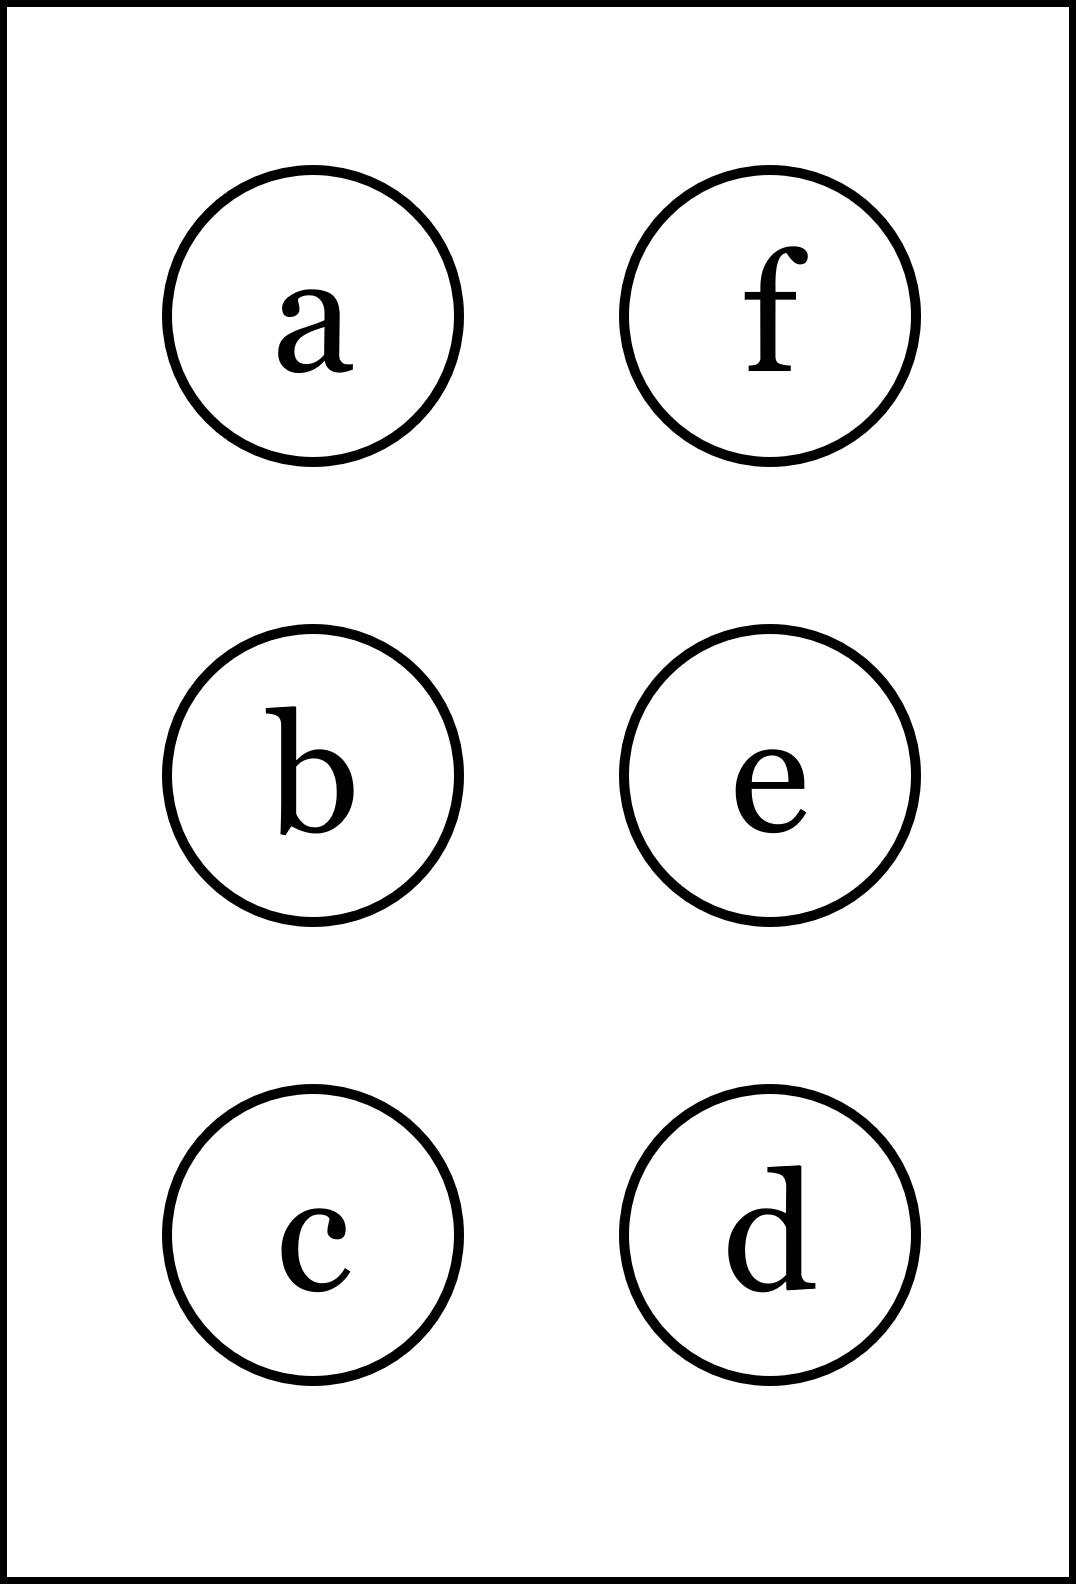
\includegraphics[height=40mm]{../images/braille.png}
{\small Písmeno Braillovej abecedy}
\end{center}
\end{minipage}
\end{center}
\end{minipage}
&
\begin{minipage}[c][104.5mm][t]{0.5\linewidth}
\begin{center}
\vspace{7mm}
{\huge Definiční obor, skupina \textit{Iota $\iota$} -\romannumeral2}\\[5mm]
\textit{Jméno:}\phantom{xxxxxxxxxxxxxxxxxxxxxxxxxxxxxxxxxxxxxxxxxxxxxxxxxxxxxxxxxxxxxxxxx}\\[5mm]
\begin{minipage}{0.95\linewidth}
\begin{center}
\textbf{Zjisti definiční obor} zadaných funkcí. Pokud se shoduje s tím za otazníky,\\tak napravo obarvi příslušející kroužek načerno. \textbf{Spolu odevzdejte výsledné slovo}.
\end{center}
\end{minipage}
\\[1mm]
\begin{minipage}{0.79\linewidth}
\begin{center}
\begin{varwidth}{\linewidth}
\begin{enumerate}
\normalsizerrr
\item $f(x)=\cfrac{4x-4}{-x-1}$\quad \dotfill\; ???\;\dotfill \quad $\mathbb{R}\smallsetminus\{-1\}$
\item $f(x)=\cfrac{1}{x^3-4x^2-11x-6}$\quad \dotfill\; ???\;\dotfill \quad $\mathbb{R}\smallsetminus\{-1,6\}$
\item $f(x)=-5\sqrt{-9x+3}$\quad \dotfill\; ???\;\dotfill \quad $x\leq\nicefrac{1}{3}$
\item $f(x)=\sqrt{-x^2+x}$\quad \dotfill\; ???\;\dotfill \quad $x\in\langle-1 , 0\rangle$
\item $f(x)=\ln{(5x-3)}$\quad \dotfill\; ???\;\dotfill \quad $x>\nicefrac{3}{5}$
\item $f(x)=\ln{(x^2-4)}$\quad \dotfill\; ???\;\dotfill \quad $x\in(-2 , 2)$
\end{enumerate}
\end{varwidth}
\end{center}
\end{minipage}
\begin{minipage}{0.20\linewidth}
\begin{center}
{\Huge\bfseries 2.} \\[2mm]
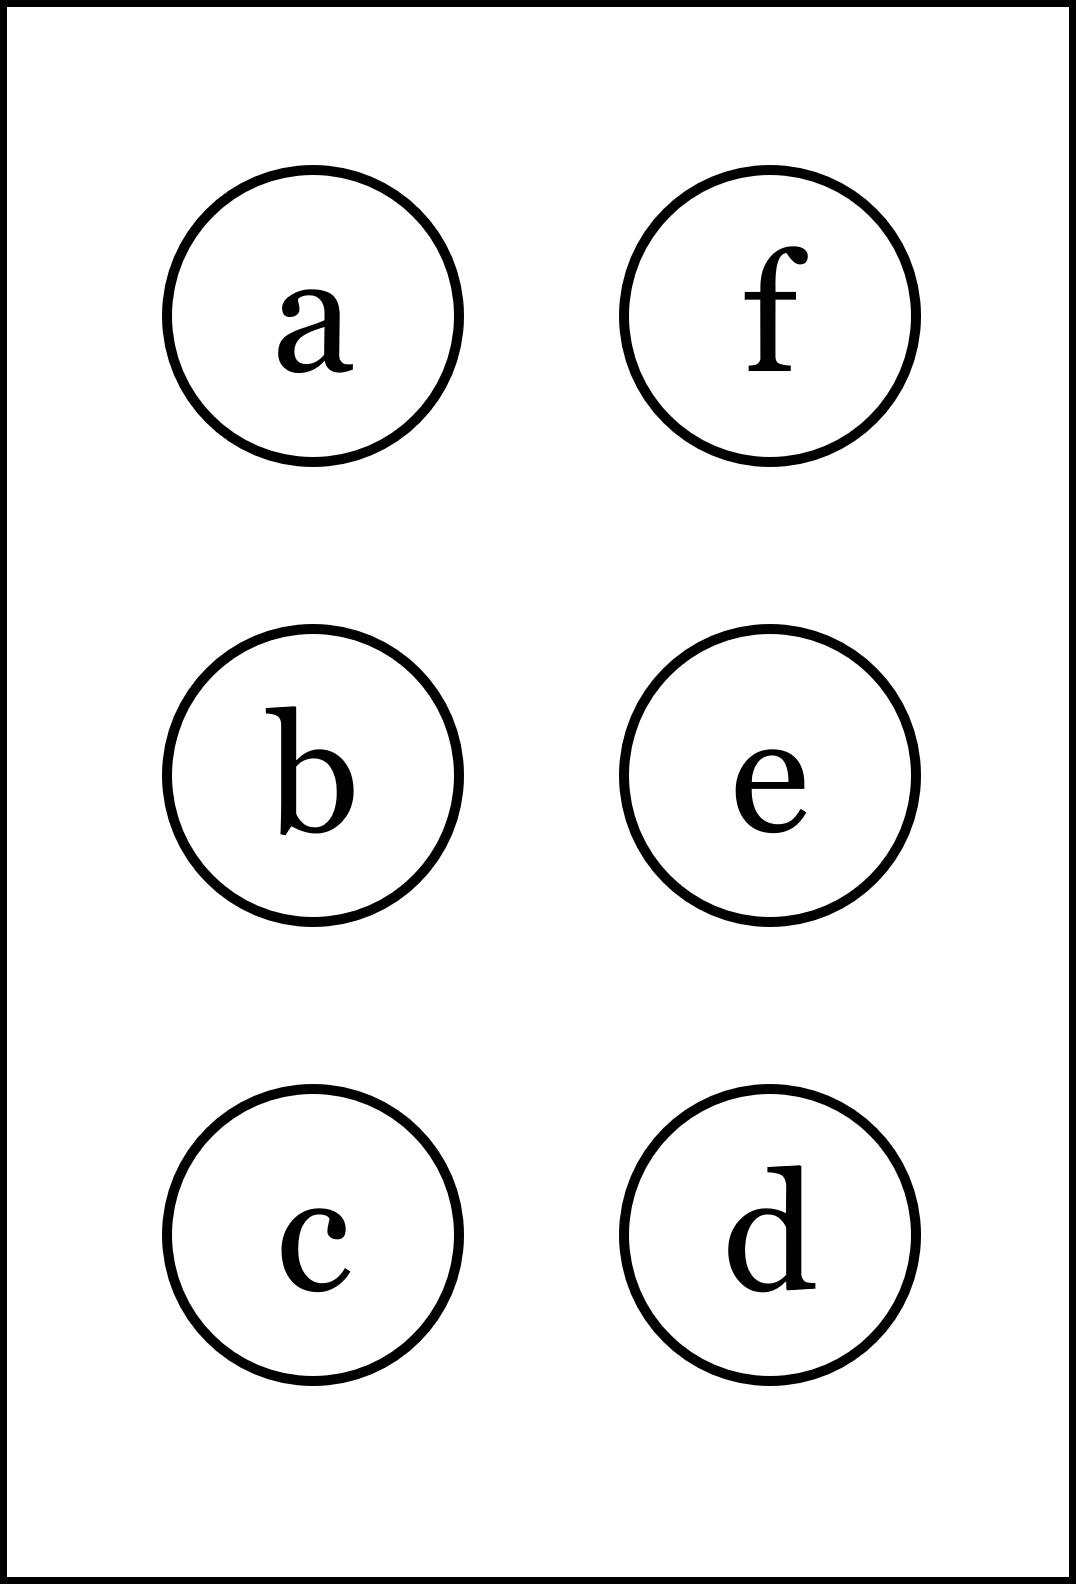
\includegraphics[height=40mm]{../images/braille.png}
{\small Písmeno Braillovej abecedy}
\end{center}
\end{minipage}
\end{center}
\end{minipage}
\\ \hdashline
\begin{minipage}[c][104.5mm][t]{0.5\linewidth}
\begin{center}
\vspace{7mm}
{\huge Definiční obor, skupina \textit{Iota $\iota$} -\romannumeral3}\\[5mm]
\textit{Jméno:}\phantom{xxxxxxxxxxxxxxxxxxxxxxxxxxxxxxxxxxxxxxxxxxxxxxxxxxxxxxxxxxxxxxxxx}\\[5mm]
\begin{minipage}{0.95\linewidth}
\begin{center}
\textbf{Zjisti definiční obor} zadaných funkcí. Pokud se shoduje s tím za otazníky,\\tak napravo obarvi příslušející kroužek načerno. \textbf{Spolu odevzdejte výsledné slovo}.
\end{center}
\end{minipage}
\\[1mm]
\begin{minipage}{0.79\linewidth}
\begin{center}
\begin{varwidth}{\linewidth}
\begin{enumerate}
\normalsizerrr
\item $f(x)=\cfrac{-x+1}{-7x-4}$\quad \dotfill\; ???\;\dotfill \quad $\mathbb{R}\smallsetminus\{\nicefrac{-4}{7}\}$
\item $f(x)=\cfrac{1}{-2x^3+14x^2+34x+18}$\quad \dotfill\; ???\;\dotfill \quad $\mathbb{R}\smallsetminus\{1,-1,7\}$
\item $f(x)=-3\sqrt{-7x-7}$\quad \dotfill\; ???\;\dotfill \quad $x\leq-1$
\item $f(x)=\sqrt{-x^2+7x}$\quad \dotfill\; ???\;\dotfill \quad $x\in(0 , 7)$
\item $f(x)=-4\ln{(-9x-1)}$\quad \dotfill\; ???\;\dotfill \quad $x<\nicefrac{-1}{9}$
\item $f(x)=\ln{(x^2+9x+8)}$\quad \dotfill\; ???\;\dotfill \quad $x\in(-\infty , -8)\cup(-1 , \infty)$
\end{enumerate}
\end{varwidth}
\end{center}
\end{minipage}
\begin{minipage}{0.20\linewidth}
\begin{center}
{\Huge\bfseries 3.} \\[2mm]
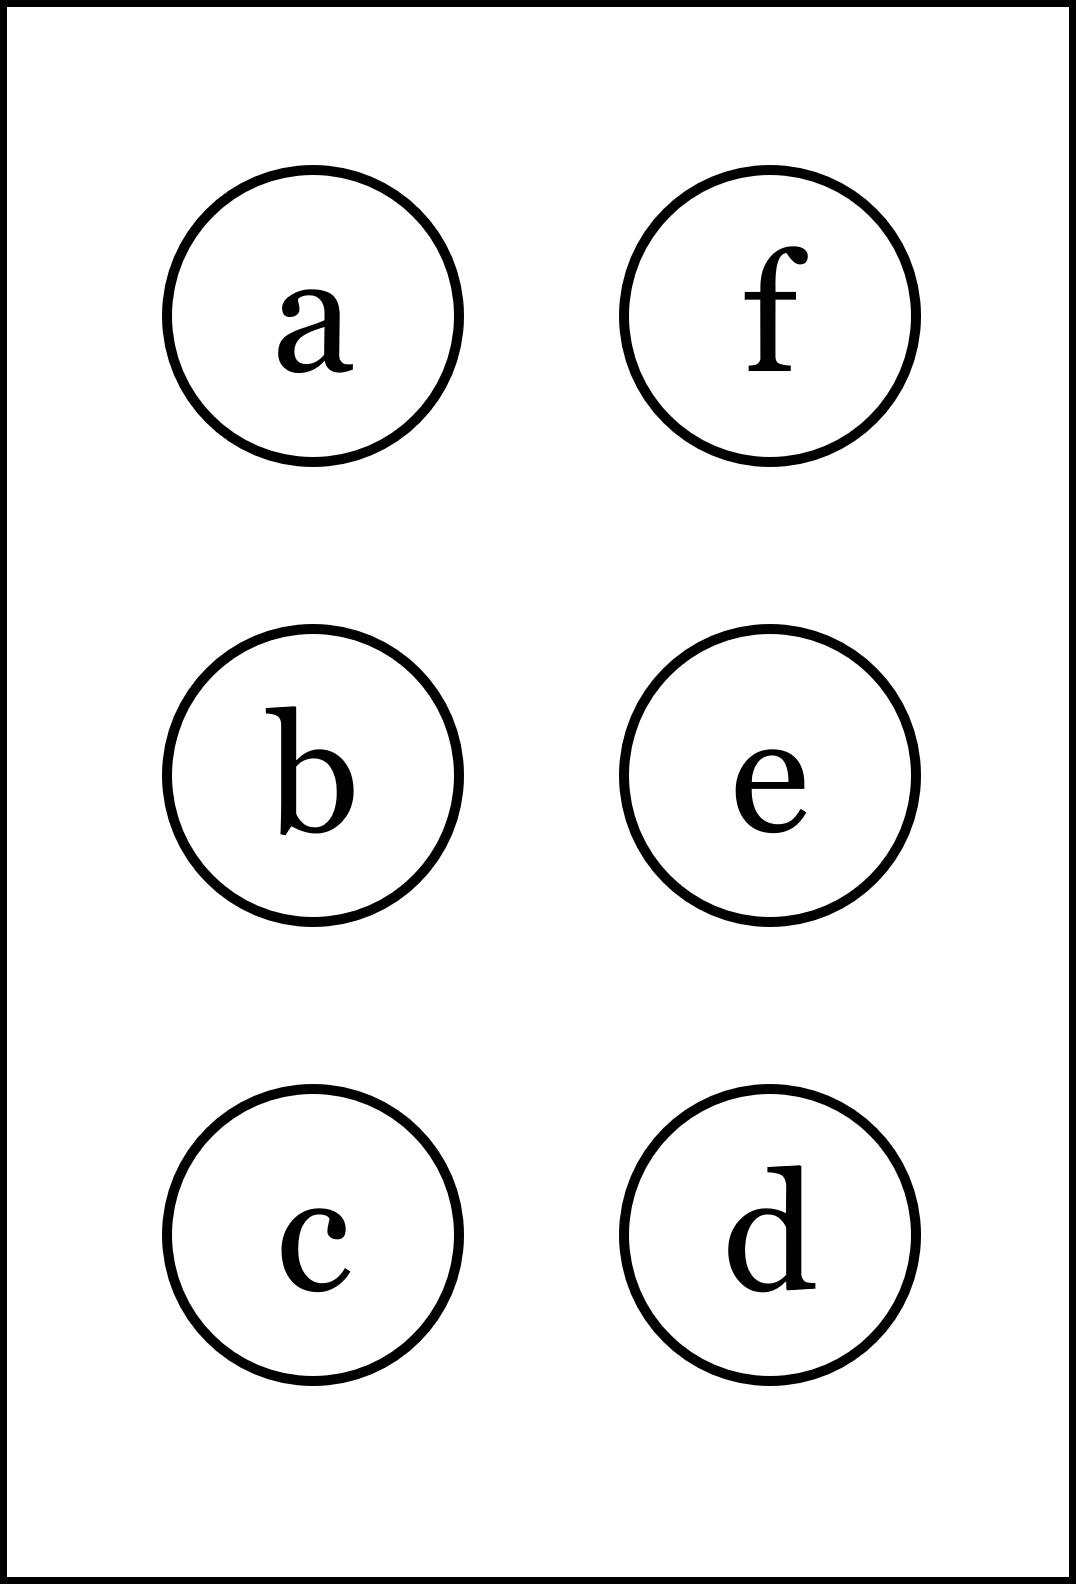
\includegraphics[height=40mm]{../images/braille.png}
{\small Písmeno Braillovej abecedy}
\end{center}
\end{minipage}
\end{center}
\end{minipage}
&
\begin{minipage}[c][104.5mm][t]{0.5\linewidth}
\begin{center}
\vspace{7mm}
{\huge Definiční obor, skupina \textit{Iota $\iota$} -\romannumeral4}\\[5mm]
\textit{Jméno:}\phantom{xxxxxxxxxxxxxxxxxxxxxxxxxxxxxxxxxxxxxxxxxxxxxxxxxxxxxxxxxxxxxxxxx}\\[5mm]
\begin{minipage}{0.95\linewidth}
\begin{center}
\textbf{Zjisti definiční obor} zadaných funkcí. Pokud se shoduje s tím za otazníky,\\tak napravo obarvi příslušející kroužek načerno. \textbf{Spolu odevzdejte výsledné slovo}.
\end{center}
\end{minipage}
\\[1mm]
\begin{minipage}{0.79\linewidth}
\begin{center}
\begin{varwidth}{\linewidth}
\begin{enumerate}
\normalsizerrr
\item $f(x)=\cfrac{-4x-1}{7x-8}$\quad \dotfill\; ???\;\dotfill \quad $\mathbb{R}\smallsetminus\{\nicefrac{8}{7}\}$
\item $f(x)=\cfrac{1}{2x^3+10x^2-2x-10}$\quad \dotfill\; ???\;\dotfill \quad $\mathbb{R}\smallsetminus\{0,-5,-1\}$
\item $f(x)=-3\sqrt{-x+2}$\quad \dotfill\; ???\;\dotfill \quad $x\leq-2$
\item $f(x)=\sqrt{-x^2-6x}$\quad \dotfill\; ???\;\dotfill \quad $x\in(-6 , 0)$
\item $f(x)=-\ln{(-6x-4)}$\quad \dotfill\; ???\;\dotfill \quad $x<\nicefrac{2}{3}$
\item $f(x)=\ln{(x^2-x-12)}$\quad \dotfill\; ???\;\dotfill \quad $x\in(-3 , 4)$
\end{enumerate}
\end{varwidth}
\end{center}
\end{minipage}
\begin{minipage}{0.20\linewidth}
\begin{center}
{\Huge\bfseries 4.} \\[2mm]
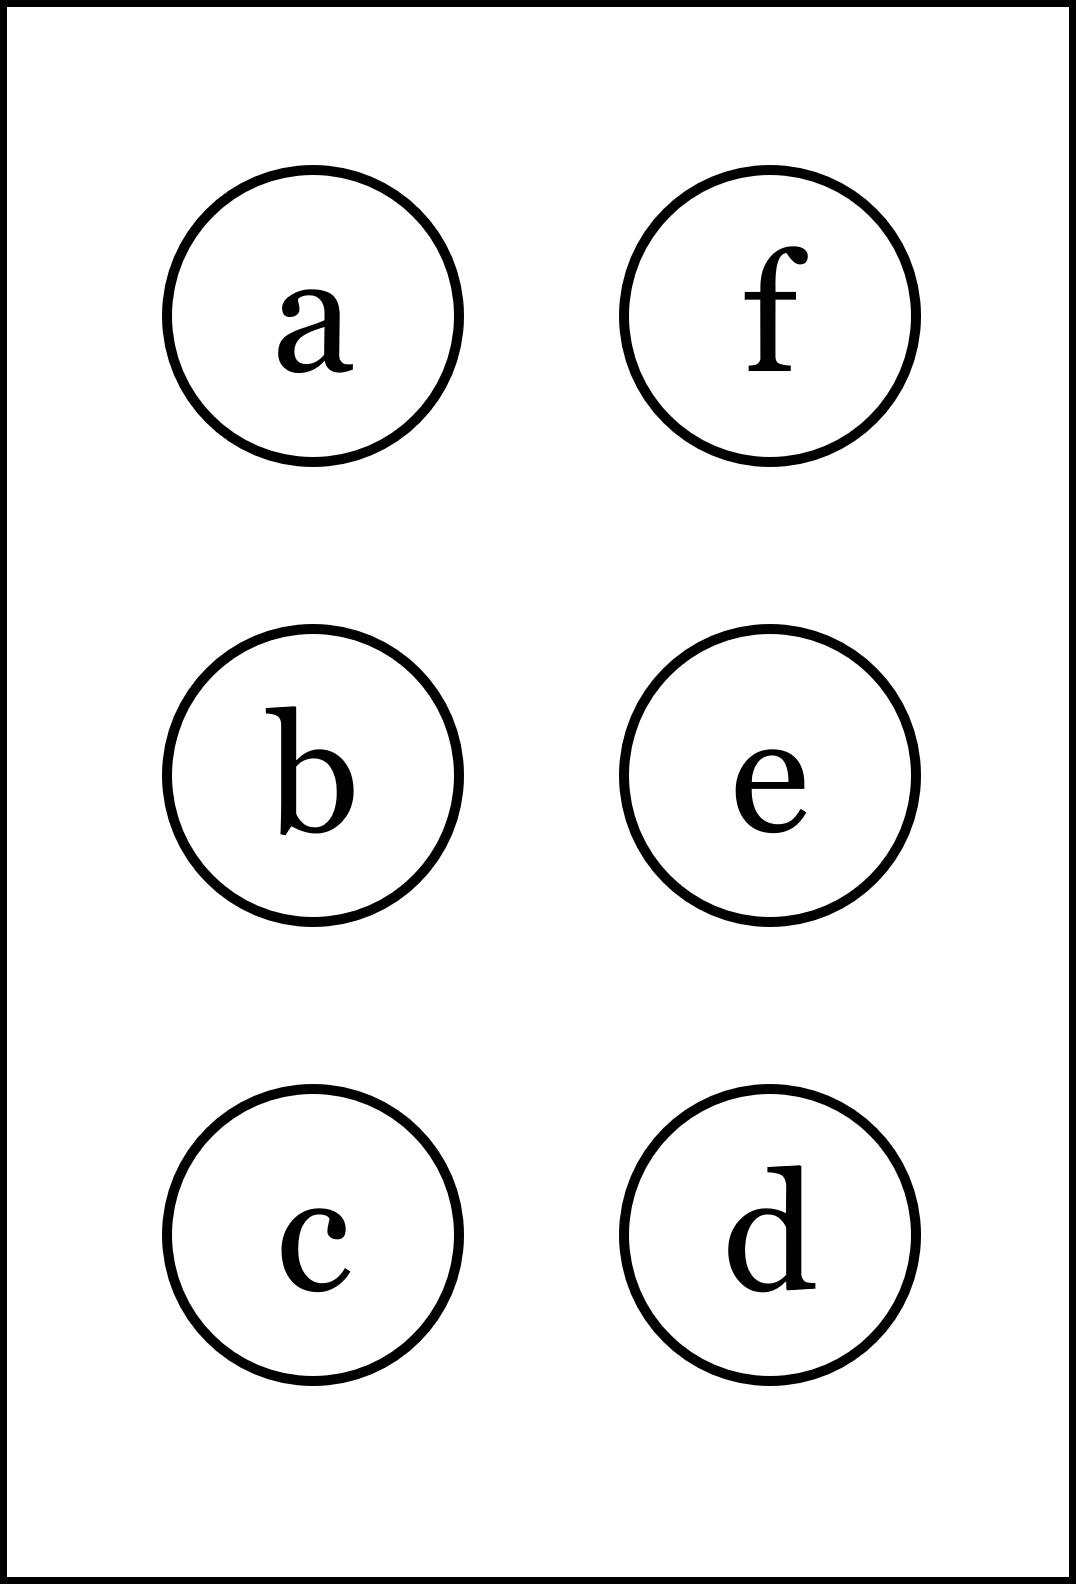
\includegraphics[height=40mm]{../images/braille.png}
{\small Písmeno Braillovej abecedy}
\end{center}
\end{minipage}
\end{center}
\end{minipage}
%
\end{tabular}
\newpage
\thispagestyle{empty}
\begin{tabular}{c:c}
\begin{minipage}[c][104.5mm][t]{0.5\linewidth}
\begin{center}
\vspace{7mm}
{\huge Definiční obor, skupina \textit{Kappa $\kappa$} -\romannumeral1}\\[5mm]
\textit{Jméno:}\phantom{xxxxxxxxxxxxxxxxxxxxxxxxxxxxxxxxxxxxxxxxxxxxxxxxxxxxxxxxxxxxxxxxx}\\[5mm]
\begin{minipage}{0.95\linewidth}
\begin{center}
\textbf{Zjisti definiční obor} zadaných funkcí. Pokud se shoduje s tím za otazníky,\\tak napravo obarvi příslušející kroužek načerno. \textbf{Spolu odevzdejte výsledné slovo}.
\end{center}
\end{minipage}
\\[1mm]
\begin{minipage}{0.79\linewidth}
\begin{center}
\begin{varwidth}{\linewidth}
\begin{enumerate}
\normalsizerrr
\item $f(x)=\cfrac{-7x+2}{-2x-1}$\quad \dotfill\; ???\;\dotfill \quad $\mathbb{R}\smallsetminus\{\nicefrac{-1}{2}\}$
\item $f(x)=\cfrac{1}{-x^3-7x^2-14x-8}$\quad \dotfill\; ???\;\dotfill \quad $\mathbb{R}\smallsetminus\{-4,-1,-2\}$
\item $f(x)=5\sqrt{6x-1}$\quad \dotfill\; ???\;\dotfill \quad $x\geq\nicefrac{1}{6}$
\item $f(x)=\sqrt{-x^2-6x}$\quad \dotfill\; ???\;\dotfill \quad $x\in\langle0 , 6\rangle$
\item $f(x)=-4\ln{(-8x-8)}$\quad \dotfill\; ???\;\dotfill \quad $x<-1$
\item $f(x)=\ln{(x^2-8x+7)}$\quad \dotfill\; ???\;\dotfill \quad $x\in(1 , 7)$
\end{enumerate}
\end{varwidth}
\end{center}
\end{minipage}
\begin{minipage}{0.20\linewidth}
\begin{center}
{\Huge\bfseries 1.} \\[2mm]
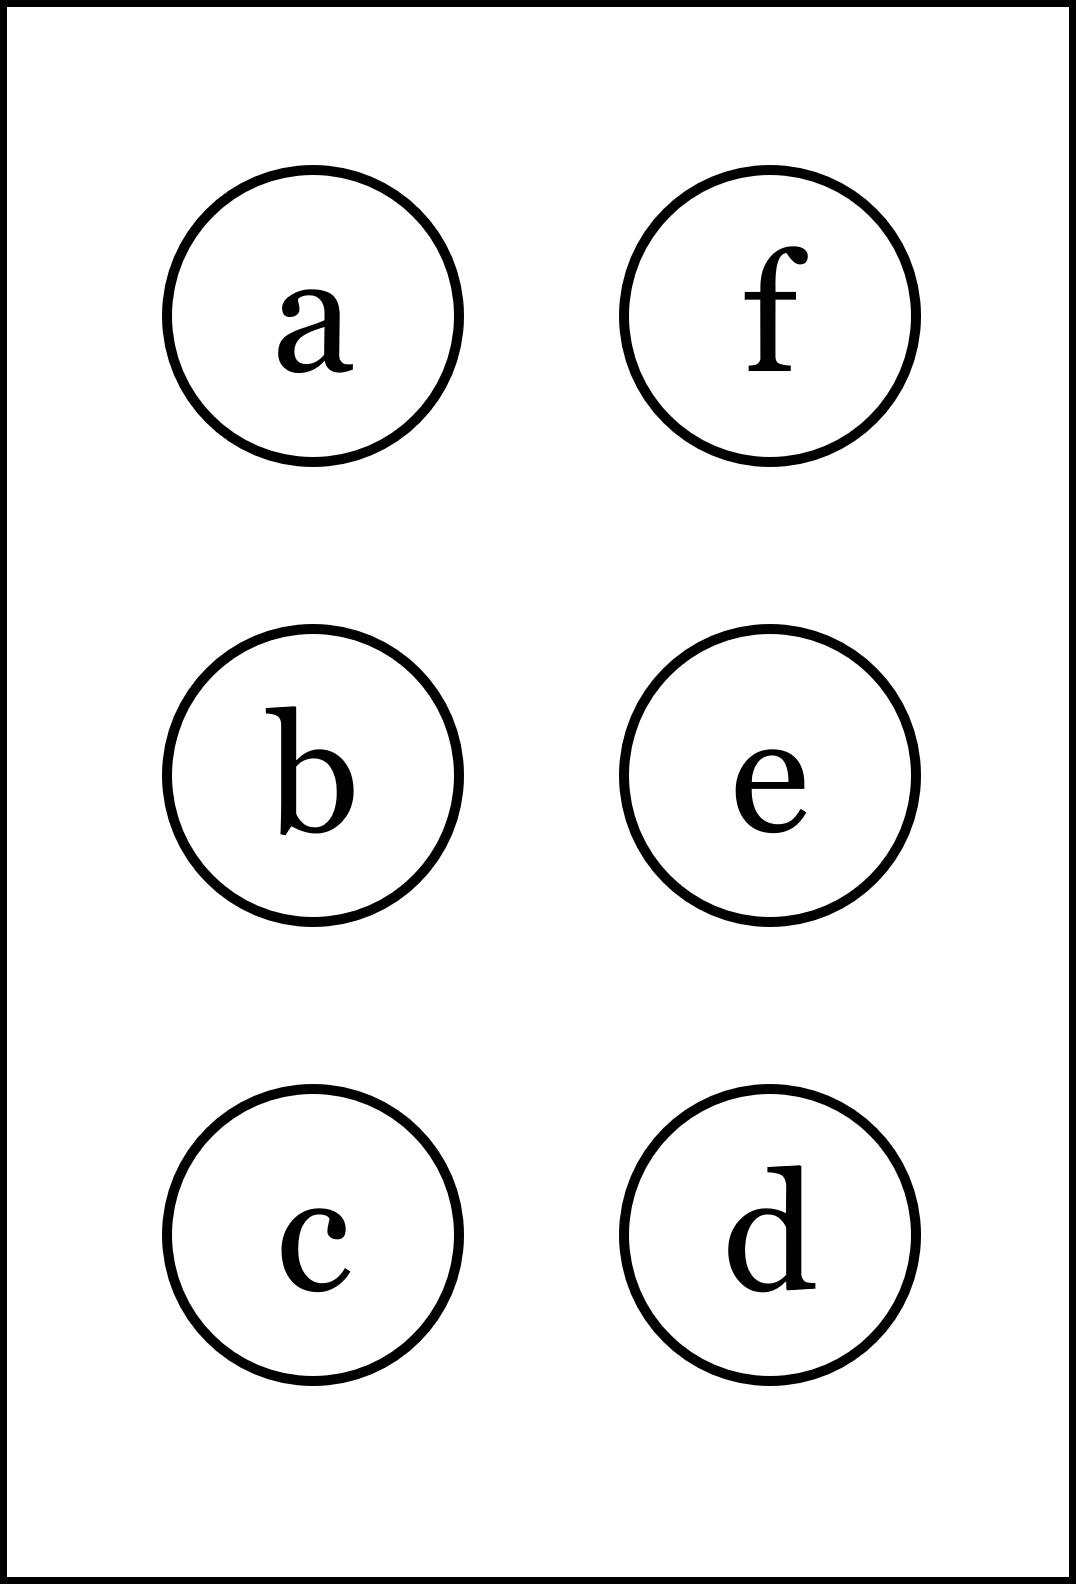
\includegraphics[height=40mm]{../images/braille.png}
{\small Písmeno Braillovej abecedy}
\end{center}
\end{minipage}
\end{center}
\end{minipage}
&
\begin{minipage}[c][104.5mm][t]{0.5\linewidth}
\begin{center}
\vspace{7mm}
{\huge Definiční obor, skupina \textit{Kappa $\kappa$} -\romannumeral2}\\[5mm]
\textit{Jméno:}\phantom{xxxxxxxxxxxxxxxxxxxxxxxxxxxxxxxxxxxxxxxxxxxxxxxxxxxxxxxxxxxxxxxxx}\\[5mm]
\begin{minipage}{0.95\linewidth}
\begin{center}
\textbf{Zjisti definiční obor} zadaných funkcí. Pokud se shoduje s tím za otazníky,\\tak napravo obarvi příslušející kroužek načerno. \textbf{Spolu odevzdejte výsledné slovo}.
\end{center}
\end{minipage}
\\[1mm]
\begin{minipage}{0.79\linewidth}
\begin{center}
\begin{varwidth}{\linewidth}
\begin{enumerate}
\normalsizerrr
\item $f(x)=\cfrac{2x-9}{3x-2}$\quad \dotfill\; ???\;\dotfill \quad $\mathbb{R}\smallsetminus\{\nicefrac{2}{3}\}$
\item $f(x)=\cfrac{1}{x^3-4x^2-19x-14}$\quad \dotfill\; ???\;\dotfill \quad $\mathbb{R}\smallsetminus\{1,5,-2\}$
\item $f(x)=-4\sqrt{-2x-6}$\quad \dotfill\; ???\;\dotfill \quad $x\geq-3$
\item $f(x)=\sqrt{-x^2-4x}$\quad \dotfill\; ???\;\dotfill \quad $x\in\langle0 , 4\rangle$
\item $f(x)=8\ln{(4x+1)}$\quad \dotfill\; ???\;\dotfill \quad $x<\nicefrac{-1}{4}$
\item $f(x)=\ln{(x^2+4x-21)}$\quad \dotfill\; ???\;\dotfill \quad $x\in(-7 , 3)$
\end{enumerate}
\end{varwidth}
\end{center}
\end{minipage}
\begin{minipage}{0.20\linewidth}
\begin{center}
{\Huge\bfseries 2.} \\[2mm]
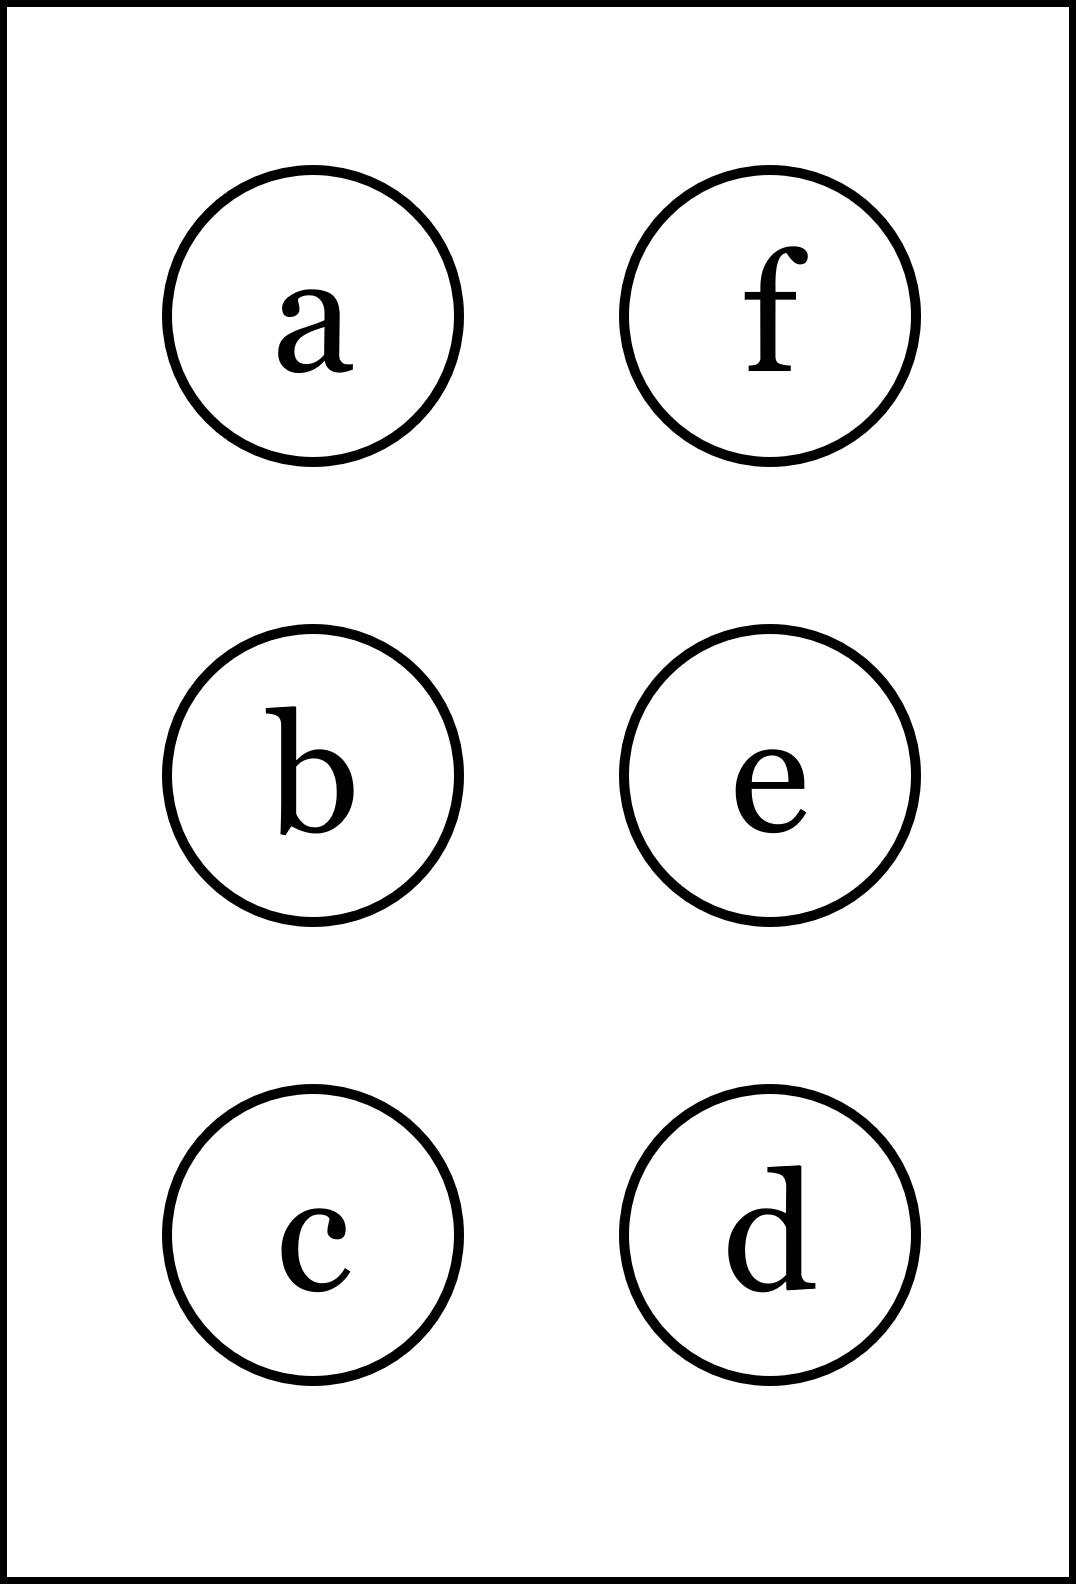
\includegraphics[height=40mm]{../images/braille.png}
{\small Písmeno Braillovej abecedy}
\end{center}
\end{minipage}
\end{center}
\end{minipage}
\\ \hdashline
\begin{minipage}[c][104.5mm][t]{0.5\linewidth}
\begin{center}
\vspace{7mm}
{\huge Definiční obor, skupina \textit{Kappa $\kappa$} -\romannumeral3}\\[5mm]
\textit{Jméno:}\phantom{xxxxxxxxxxxxxxxxxxxxxxxxxxxxxxxxxxxxxxxxxxxxxxxxxxxxxxxxxxxxxxxxx}\\[5mm]
\begin{minipage}{0.95\linewidth}
\begin{center}
\textbf{Zjisti definiční obor} zadaných funkcí. Pokud se shoduje s tím za otazníky,\\tak napravo obarvi příslušející kroužek načerno. \textbf{Spolu odevzdejte výsledné slovo}.
\end{center}
\end{minipage}
\\[1mm]
\begin{minipage}{0.79\linewidth}
\begin{center}
\begin{varwidth}{\linewidth}
\begin{enumerate}
\normalsizerrr
\item $f(x)=\cfrac{-x+5}{-6x-5}$\quad \dotfill\; ???\;\dotfill \quad $\mathbb{R}\smallsetminus\{\nicefrac{-5}{6}\}$
\item $f(x)=\cfrac{1}{2x^3-12x^2+22x-12}$\quad \dotfill\; ???\;\dotfill \quad $\mathbb{R}\smallsetminus\{3,4,-1\}$
\item $f(x)=2\sqrt{2x+4}$\quad \dotfill\; ???\;\dotfill \quad $x\leq-2$
\item $f(x)=\sqrt{-x^2+4x}$\quad \dotfill\; ???\;\dotfill \quad $x\in(0 , 4)$
\item $f(x)=4\ln{(5x-7)}$\quad \dotfill\; ???\;\dotfill \quad $x>\nicefrac{7}{5}$
\item $f(x)=\ln{(x^2-11x+24)}$\quad \dotfill\; ???\;\dotfill \quad $x\in(-\infty , 3)\cup(8 , \infty)$
\end{enumerate}
\end{varwidth}
\end{center}
\end{minipage}
\begin{minipage}{0.20\linewidth}
\begin{center}
{\Huge\bfseries 3.} \\[2mm]
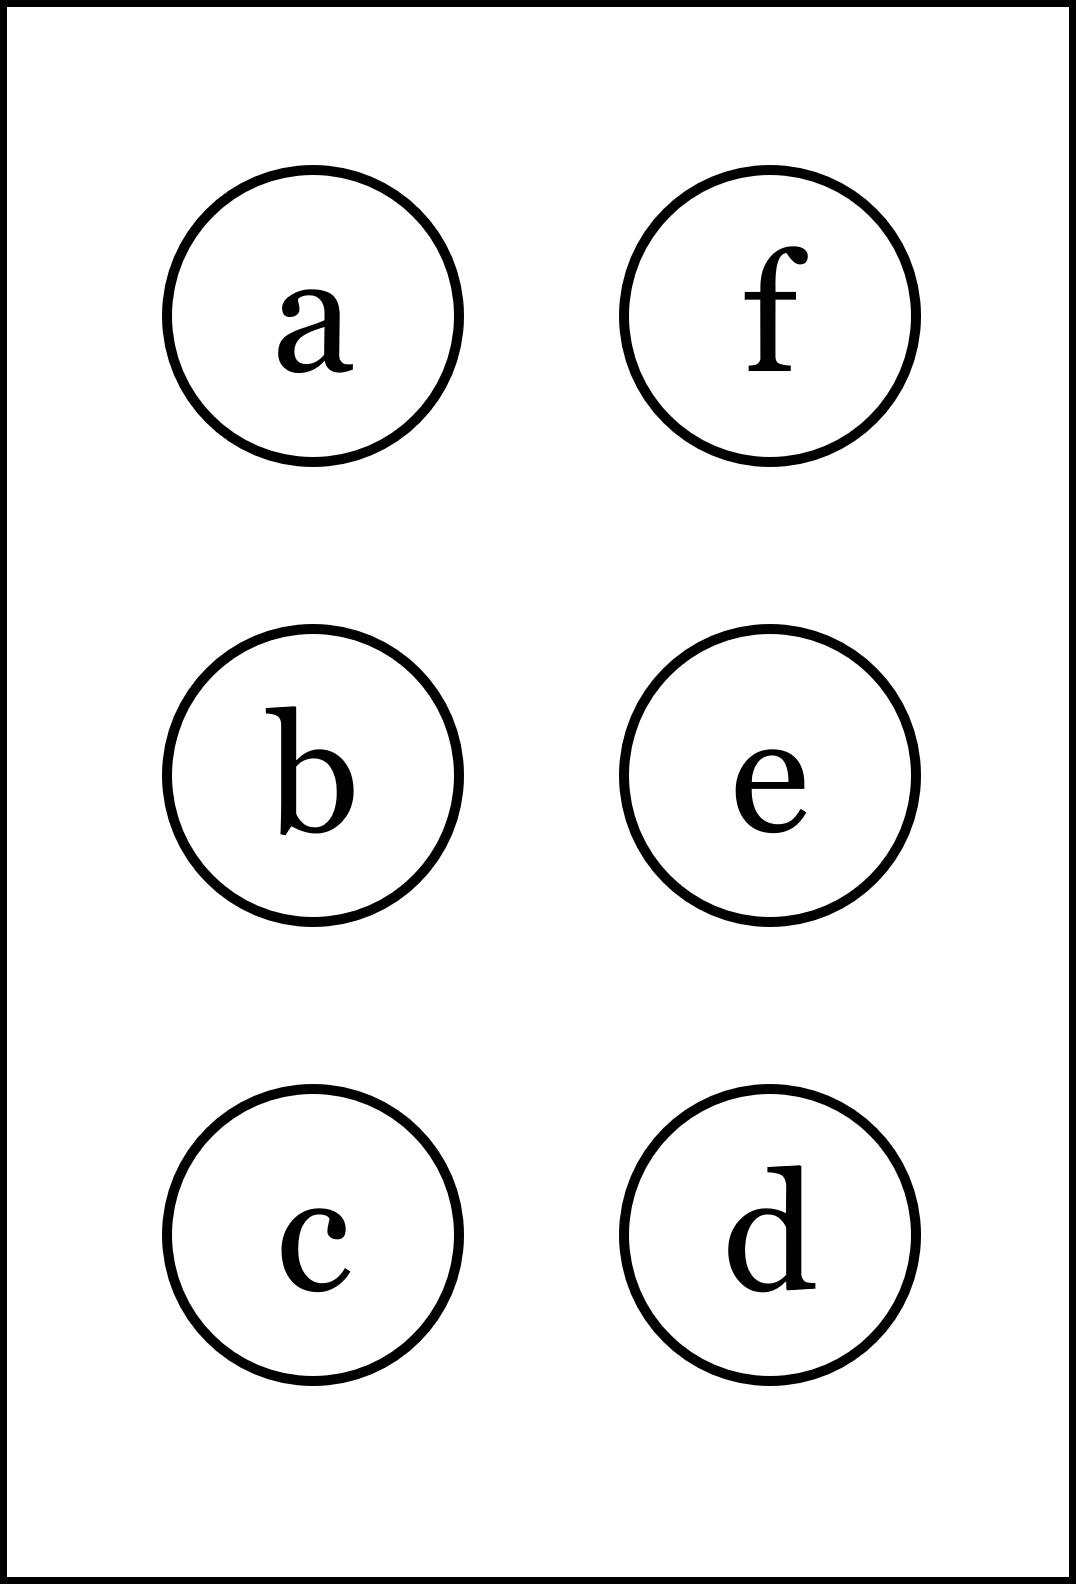
\includegraphics[height=40mm]{../images/braille.png}
{\small Písmeno Braillovej abecedy}
\end{center}
\end{minipage}
\end{center}
\end{minipage}
&
\begin{minipage}[c][104.5mm][t]{0.5\linewidth}
\begin{center}
\vspace{7mm}
{\huge Definiční obor, skupina \textit{Kappa $\kappa$} -\romannumeral4}\\[5mm]
\textit{Jméno:}\phantom{xxxxxxxxxxxxxxxxxxxxxxxxxxxxxxxxxxxxxxxxxxxxxxxxxxxxxxxxxxxxxxxxx}\\[5mm]
\begin{minipage}{0.95\linewidth}
\begin{center}
\textbf{Zjisti definiční obor} zadaných funkcí. Pokud se shoduje s tím za otazníky,\\tak napravo obarvi příslušející kroužek načerno. \textbf{Spolu odevzdejte výsledné slovo}.
\end{center}
\end{minipage}
\\[1mm]
\begin{minipage}{0.79\linewidth}
\begin{center}
\begin{varwidth}{\linewidth}
\begin{enumerate}
\normalsizerrr
\item $f(x)=\cfrac{2x-4}{x-6}$\quad \dotfill\; ???\;\dotfill \quad $\mathbb{R}\smallsetminus\{6\}$
\item $f(x)=\cfrac{1}{-5x^3+15x^2-15x+5}$\quad \dotfill\; ???\;\dotfill \quad $\mathbb{R}\smallsetminus\{1,2,-1\}$
\item $f(x)=-2\sqrt{-3x-1}$\quad \dotfill\; ???\;\dotfill \quad $x\geq\nicefrac{-1}{3}$
\item $f(x)=\sqrt{-x^2-7x}$\quad \dotfill\; ???\;\dotfill \quad $x\in(-7 , 0)$
\item $f(x)=-2\ln{(2x-2)}$\quad \dotfill\; ???\;\dotfill \quad $x<1$
\item $f(x)=\ln{(x^2-64)}$\quad \dotfill\; ???\;\dotfill \quad $x\in(-8 , 8)$
\end{enumerate}
\end{varwidth}
\end{center}
\end{minipage}
\begin{minipage}{0.20\linewidth}
\begin{center}
{\Huge\bfseries 4.} \\[2mm]
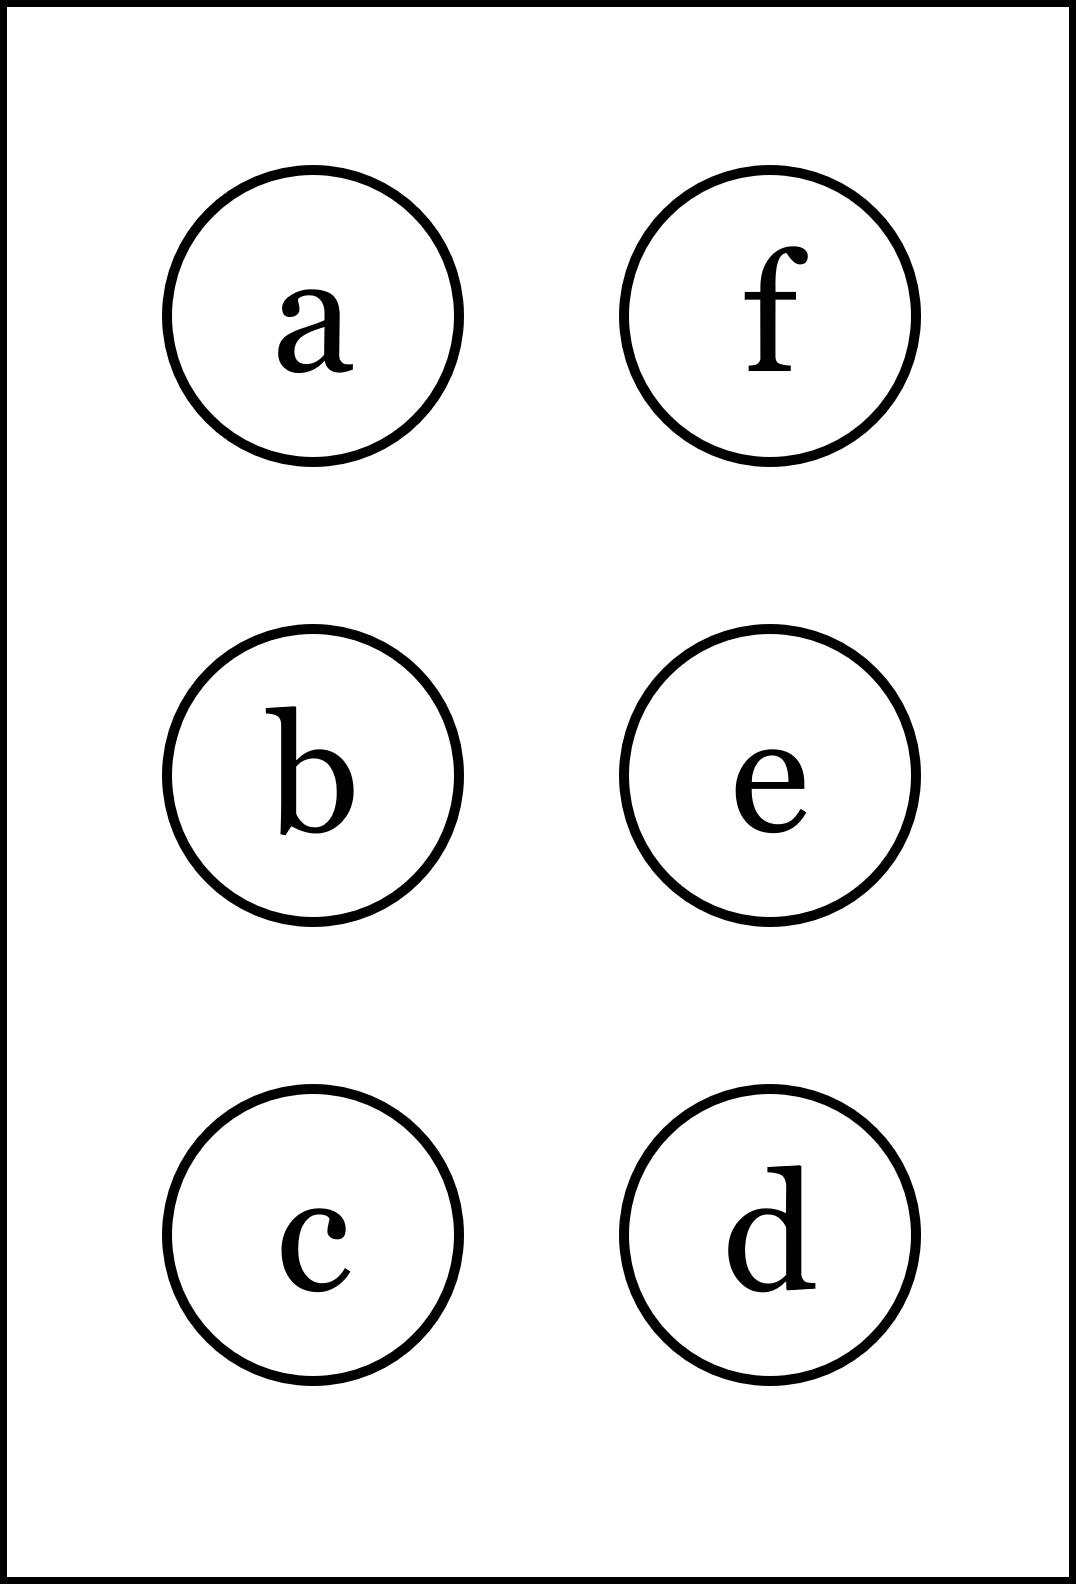
\includegraphics[height=40mm]{../images/braille.png}
{\small Písmeno Braillovej abecedy}
\end{center}
\end{minipage}
\end{center}
\end{minipage}
%
\end{tabular}
\newpage
\thispagestyle{empty}
\begin{tabular}{c:c}
\begin{minipage}[c][104.5mm][t]{0.5\linewidth}
\begin{center}
\vspace{7mm}
{\huge Definiční obor, skupina \textit{Lambda $\lambda$} -\romannumeral1}\\[5mm]
\textit{Jméno:}\phantom{xxxxxxxxxxxxxxxxxxxxxxxxxxxxxxxxxxxxxxxxxxxxxxxxxxxxxxxxxxxxxxxxx}\\[5mm]
\begin{minipage}{0.95\linewidth}
\begin{center}
\textbf{Zjisti definiční obor} zadaných funkcí. Pokud se shoduje s tím za otazníky,\\tak napravo obarvi příslušející kroužek načerno. \textbf{Spolu odevzdejte výsledné slovo}.
\end{center}
\end{minipage}
\\[1mm]
\begin{minipage}{0.79\linewidth}
\begin{center}
\begin{varwidth}{\linewidth}
\begin{enumerate}
\normalsizerrr
\item $f(x)=\cfrac{-2x-8}{-2x+4}$\quad \dotfill\; ???\;\dotfill \quad $\mathbb{R}\smallsetminus\{2\}$
\item $f(x)=\cfrac{1}{x^3-7x-6}$\quad \dotfill\; ???\;\dotfill \quad $\mathbb{R}\smallsetminus\{3,-2,-1\}$
\item $f(x)=-\sqrt{-3x-3}$\quad \dotfill\; ???\;\dotfill \quad $x\leq-1$
\item $f(x)=\sqrt{-x^2+2x}$\quad \dotfill\; ???\;\dotfill \quad $x\in\langle0 , 2\rangle$
\item $f(x)=2\ln{(-6x-4)}$\quad \dotfill\; ???\;\dotfill \quad $x<\nicefrac{-2}{3}$
\item $f(x)=\ln{(x^2-3x-10)}$\quad \dotfill\; ???\;\dotfill \quad $x\in(-2 , 5)$
\end{enumerate}
\end{varwidth}
\end{center}
\end{minipage}
\begin{minipage}{0.20\linewidth}
\begin{center}
{\Huge\bfseries 1.} \\[2mm]
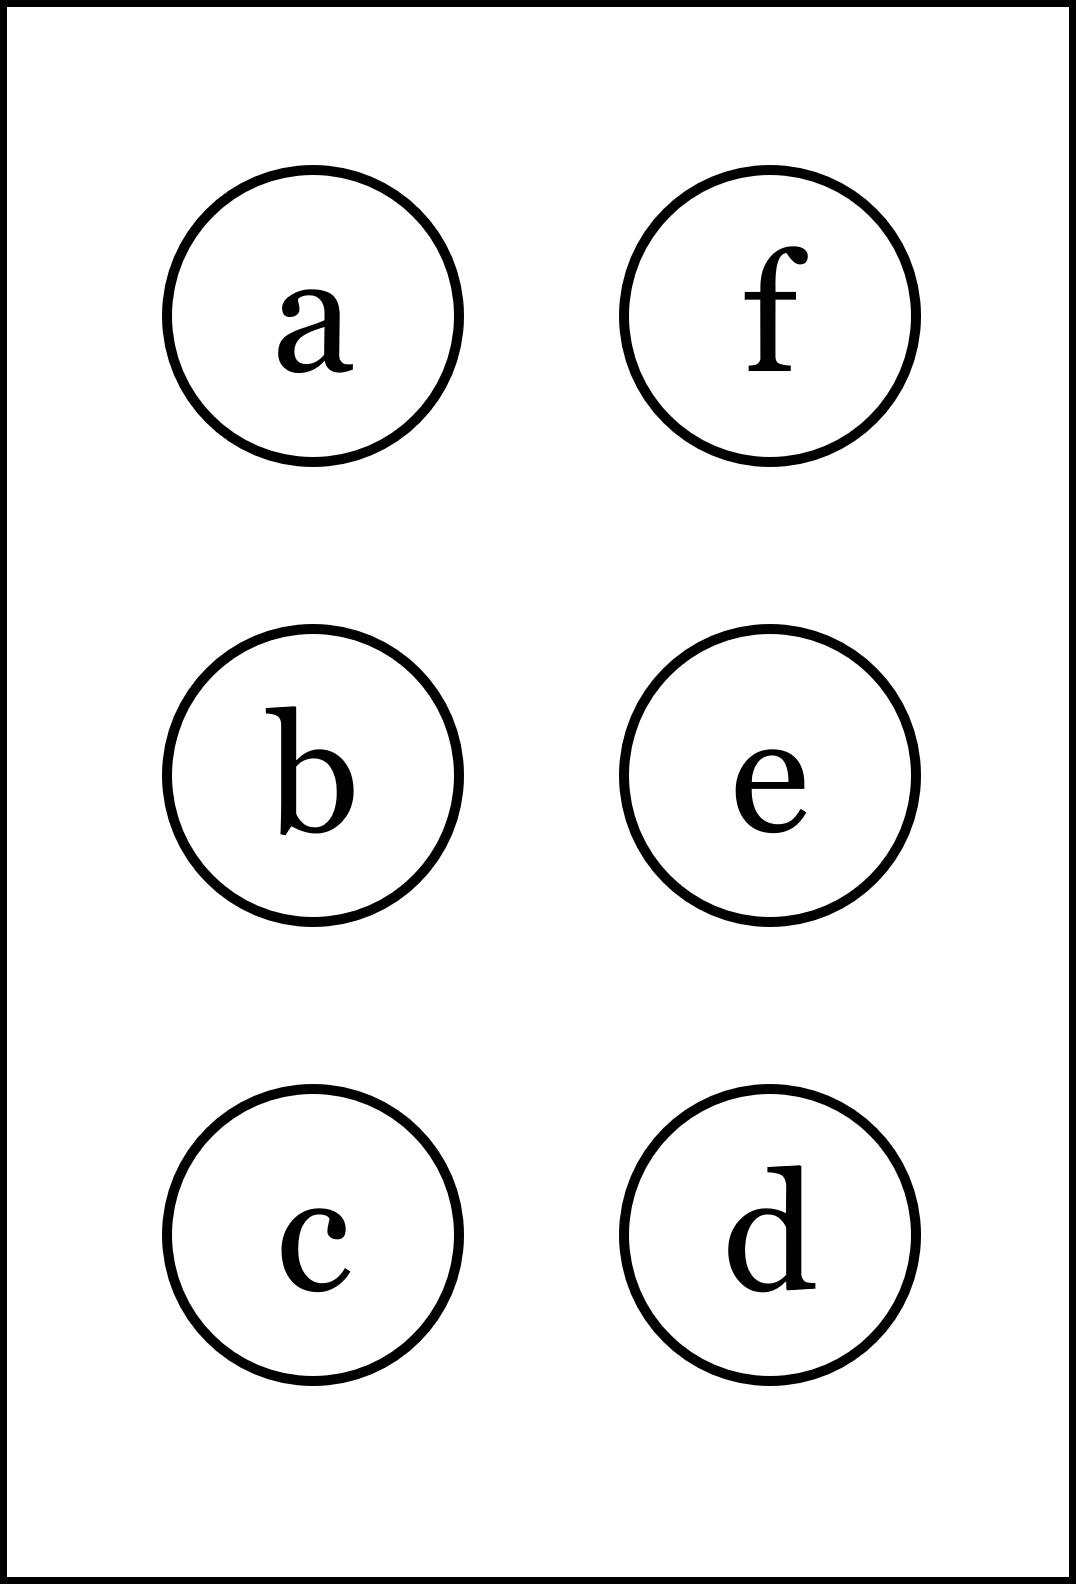
\includegraphics[height=40mm]{../images/braille.png}
{\small Písmeno Braillovej abecedy}
\end{center}
\end{minipage}
\end{center}
\end{minipage}
&
\begin{minipage}[c][104.5mm][t]{0.5\linewidth}
\begin{center}
\vspace{7mm}
{\huge Definiční obor, skupina \textit{Lambda $\lambda$} -\romannumeral2}\\[5mm]
\textit{Jméno:}\phantom{xxxxxxxxxxxxxxxxxxxxxxxxxxxxxxxxxxxxxxxxxxxxxxxxxxxxxxxxxxxxxxxxx}\\[5mm]
\begin{minipage}{0.95\linewidth}
\begin{center}
\textbf{Zjisti definiční obor} zadaných funkcí. Pokud se shoduje s tím za otazníky,\\tak napravo obarvi příslušející kroužek načerno. \textbf{Spolu odevzdejte výsledné slovo}.
\end{center}
\end{minipage}
\\[1mm]
\begin{minipage}{0.79\linewidth}
\begin{center}
\begin{varwidth}{\linewidth}
\begin{enumerate}
\normalsizerrr
\item $f(x)=\cfrac{9x+3}{x-1}$\quad \dotfill\; ???\;\dotfill \quad $\mathbb{R}\smallsetminus\{1\}$
\item $f(x)=\cfrac{1}{x^3-5x^2-17x+21}$\quad \dotfill\; ???\;\dotfill \quad $\mathbb{R}\smallsetminus\{-5,-1,7\}$
\item $f(x)=-4\sqrt{6x+5}$\quad \dotfill\; ???\;\dotfill \quad $x\geq\nicefrac{-5}{6}$
\item $f(x)=\sqrt{-x^2-2x}$\quad \dotfill\; ???\;\dotfill \quad $x\in\langle0 , 2\rangle$
\item $f(x)=-\ln{(x-5)}$\quad \dotfill\; ???\;\dotfill \quad $x>5$
\item $f(x)=\ln{(x^2+2x-3)}$\quad \dotfill\; ???\;\dotfill \quad $x\in(-3 , 1)$
\end{enumerate}
\end{varwidth}
\end{center}
\end{minipage}
\begin{minipage}{0.20\linewidth}
\begin{center}
{\Huge\bfseries 2.} \\[2mm]
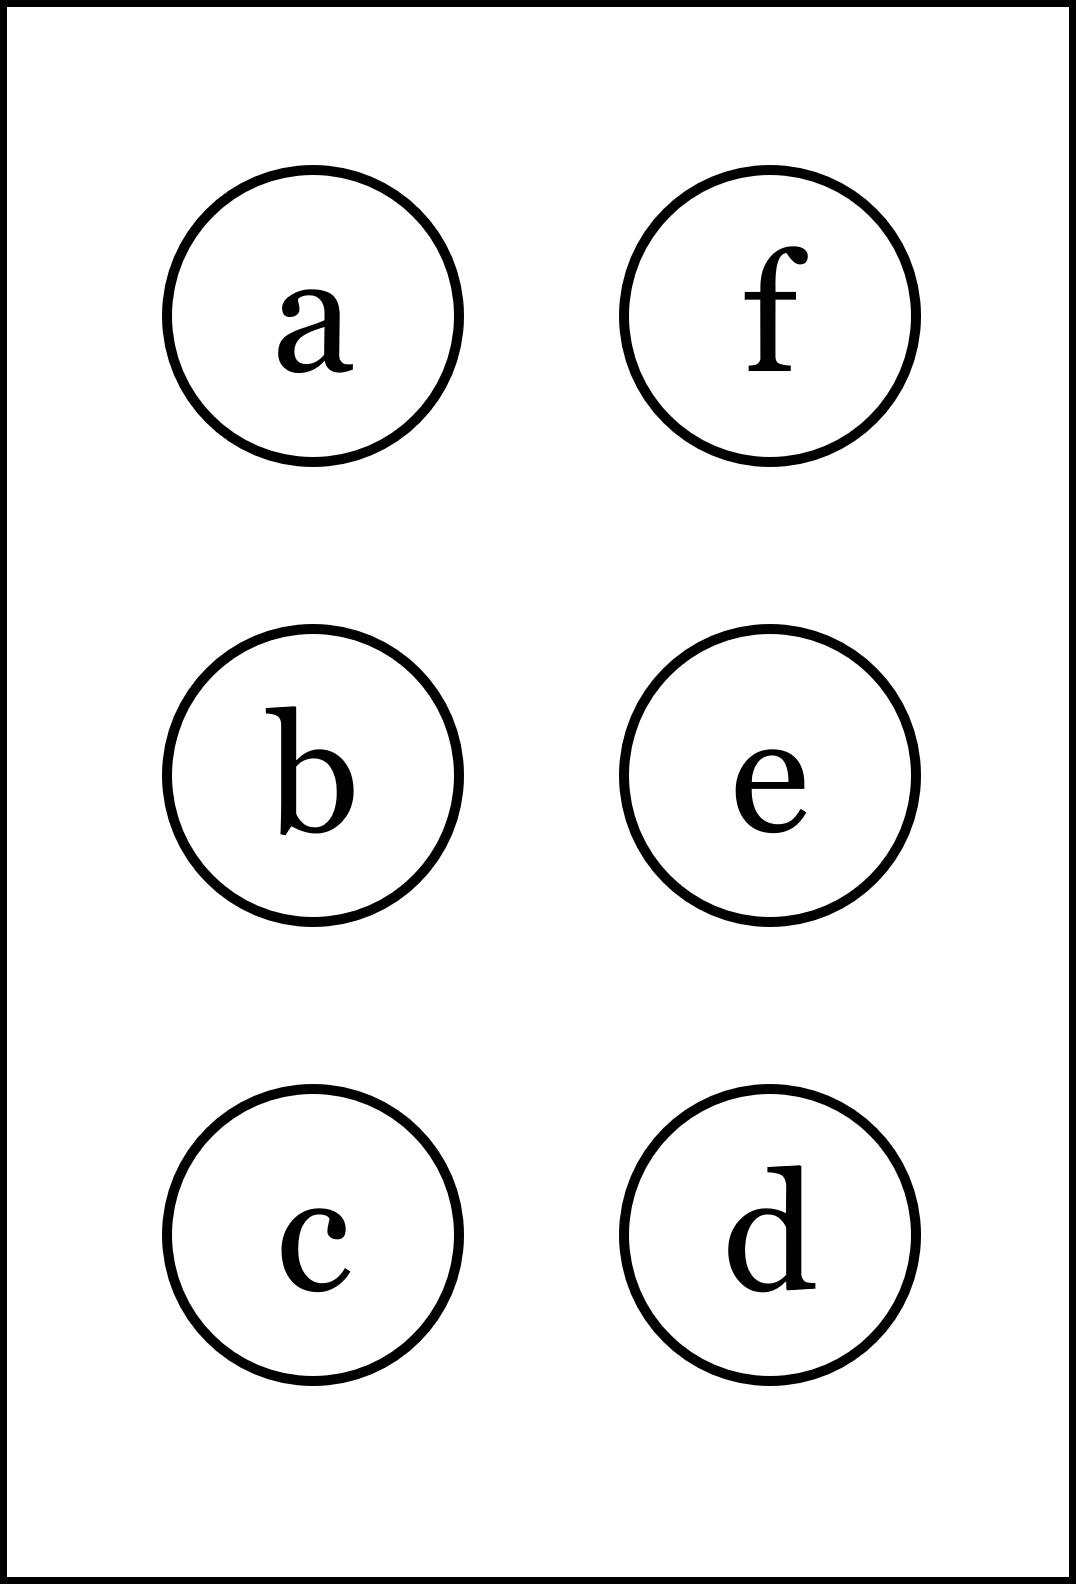
\includegraphics[height=40mm]{../images/braille.png}
{\small Písmeno Braillovej abecedy}
\end{center}
\end{minipage}
\end{center}
\end{minipage}
\\ \hdashline
\begin{minipage}[c][104.5mm][t]{0.5\linewidth}
\begin{center}
\vspace{7mm}
{\huge Definiční obor, skupina \textit{Lambda $\lambda$} -\romannumeral3}\\[5mm]
\textit{Jméno:}\phantom{xxxxxxxxxxxxxxxxxxxxxxxxxxxxxxxxxxxxxxxxxxxxxxxxxxxxxxxxxxxxxxxxx}\\[5mm]
\begin{minipage}{0.95\linewidth}
\begin{center}
\textbf{Zjisti definiční obor} zadaných funkcí. Pokud se shoduje s tím za otazníky,\\tak napravo obarvi příslušející kroužek načerno. \textbf{Spolu odevzdejte výsledné slovo}.
\end{center}
\end{minipage}
\\[1mm]
\begin{minipage}{0.79\linewidth}
\begin{center}
\begin{varwidth}{\linewidth}
\begin{enumerate}
\normalsizerrr
\item $f(x)=\cfrac{3x+4}{x-3}$\quad \dotfill\; ???\;\dotfill \quad $\mathbb{R}\smallsetminus\{3\}$
\item $f(x)=\cfrac{1}{-2x^3-18x^2-22x+42}$\quad \dotfill\; ???\;\dotfill \quad $\mathbb{R}\smallsetminus\{-7,-3,1\}$
\item $f(x)=-5\sqrt{7x-3}$\quad \dotfill\; ???\;\dotfill \quad $x\geq\nicefrac{3}{7}$
\item $f(x)=\sqrt{-x^2-9x}$\quad \dotfill\; ???\;\dotfill \quad $x\in\langle0 , 9\rangle$
\item $f(x)=5\ln{(-7x+1)}$\quad \dotfill\; ???\;\dotfill \quad $x>\nicefrac{1}{7}$
\item $f(x)=\ln{(x^2-8x+15)}$\quad \dotfill\; ???\;\dotfill \quad $x\in(3 , 5)$
\end{enumerate}
\end{varwidth}
\end{center}
\end{minipage}
\begin{minipage}{0.20\linewidth}
\begin{center}
{\Huge\bfseries 3.} \\[2mm]
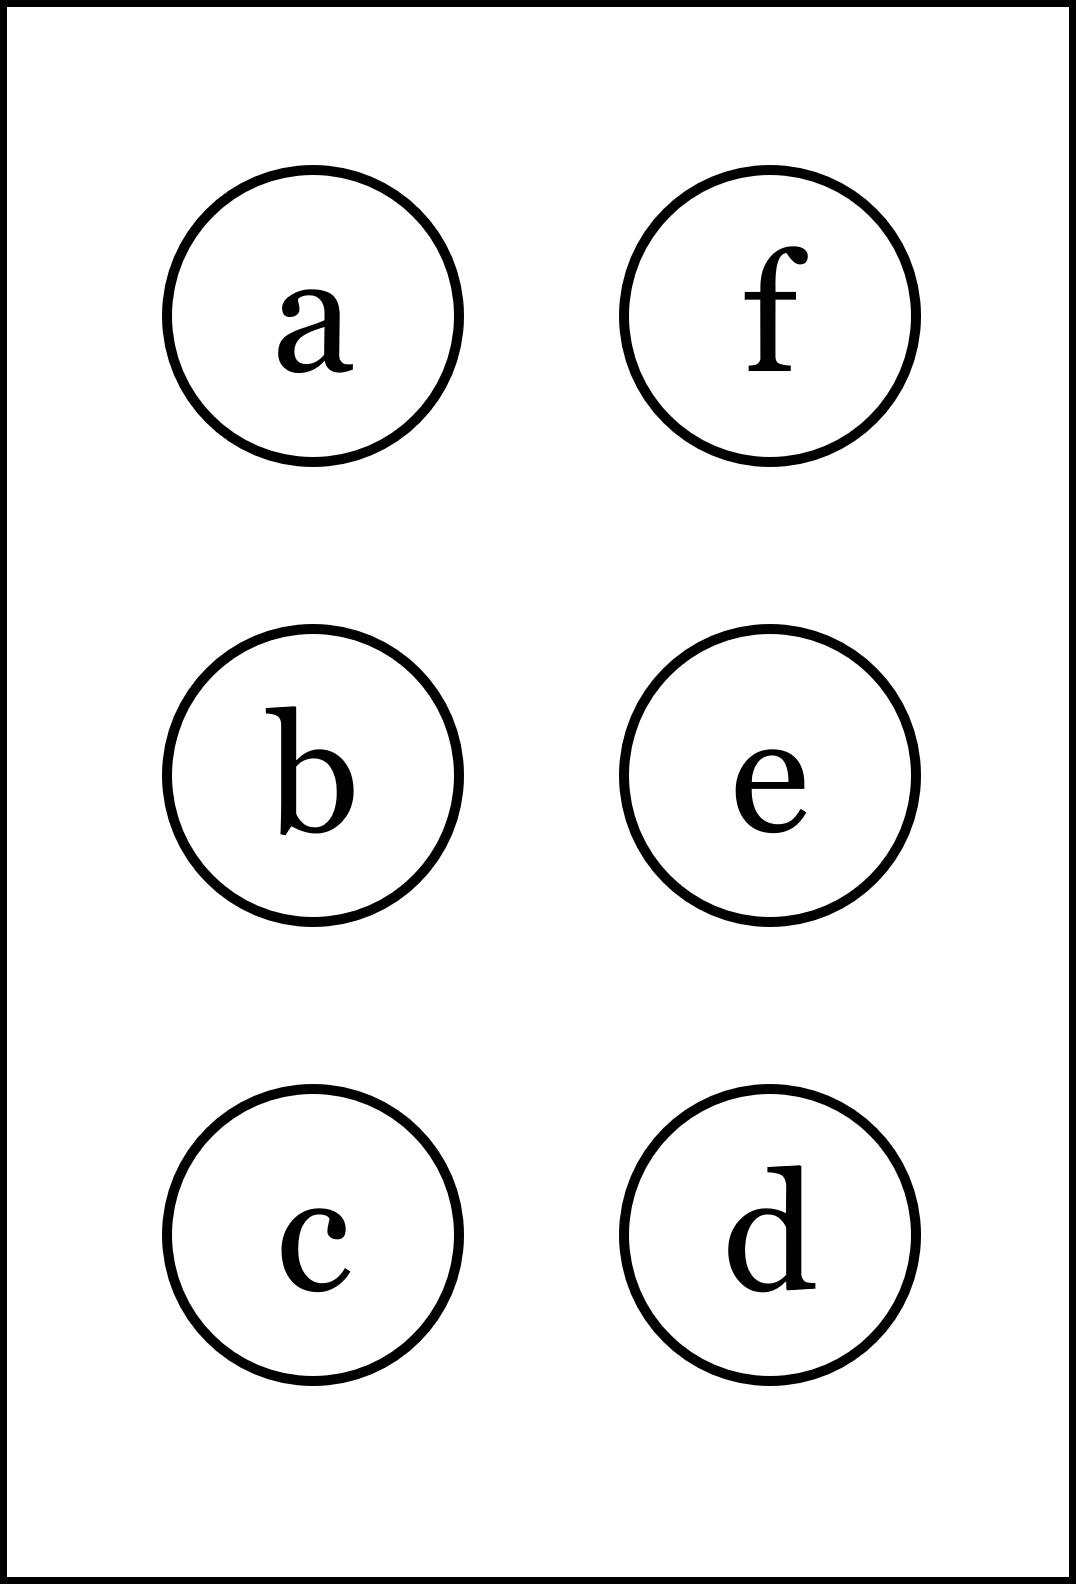
\includegraphics[height=40mm]{../images/braille.png}
{\small Písmeno Braillovej abecedy}
\end{center}
\end{minipage}
\end{center}
\end{minipage}
&
\begin{minipage}[c][104.5mm][t]{0.5\linewidth}
\begin{center}
\vspace{7mm}
{\huge Definiční obor, skupina \textit{Lambda $\lambda$} -\romannumeral4}\\[5mm]
\textit{Jméno:}\phantom{xxxxxxxxxxxxxxxxxxxxxxxxxxxxxxxxxxxxxxxxxxxxxxxxxxxxxxxxxxxxxxxxx}\\[5mm]
\begin{minipage}{0.95\linewidth}
\begin{center}
\textbf{Zjisti definiční obor} zadaných funkcí. Pokud se shoduje s tím za otazníky,\\tak napravo obarvi příslušející kroužek načerno. \textbf{Spolu odevzdejte výsledné slovo}.
\end{center}
\end{minipage}
\\[1mm]
\begin{minipage}{0.79\linewidth}
\begin{center}
\begin{varwidth}{\linewidth}
\begin{enumerate}
\normalsizerrr
\item $f(x)=\cfrac{6x-8}{x+8}$\quad \dotfill\; ???\;\dotfill \quad $\mathbb{R}\smallsetminus\{-8\}$
\item $f(x)=\cfrac{1}{-5x^3-35x^2-70x-40}$\quad \dotfill\; ???\;\dotfill \quad $\mathbb{R}\smallsetminus\{-4,-1,-2\}$
\item $f(x)=6\sqrt{-x-1}$\quad \dotfill\; ???\;\dotfill \quad $x\geq-1$
\item $f(x)=\sqrt{-x^2+9x}$\quad \dotfill\; ???\;\dotfill \quad $x\in\langle-9 , 0\rangle$
\item $f(x)=5\ln{(7x+5)}$\quad \dotfill\; ???\;\dotfill \quad $x<\nicefrac{-5}{7}$
\item $f(x)=\ln{(x^2-10x+9)}$\quad \dotfill\; ???\;\dotfill \quad $x\in(-\infty , 1)\cup(9 , \infty)$
\end{enumerate}
\end{varwidth}
\end{center}
\end{minipage}
\begin{minipage}{0.20\linewidth}
\begin{center}
{\Huge\bfseries 4.} \\[2mm]
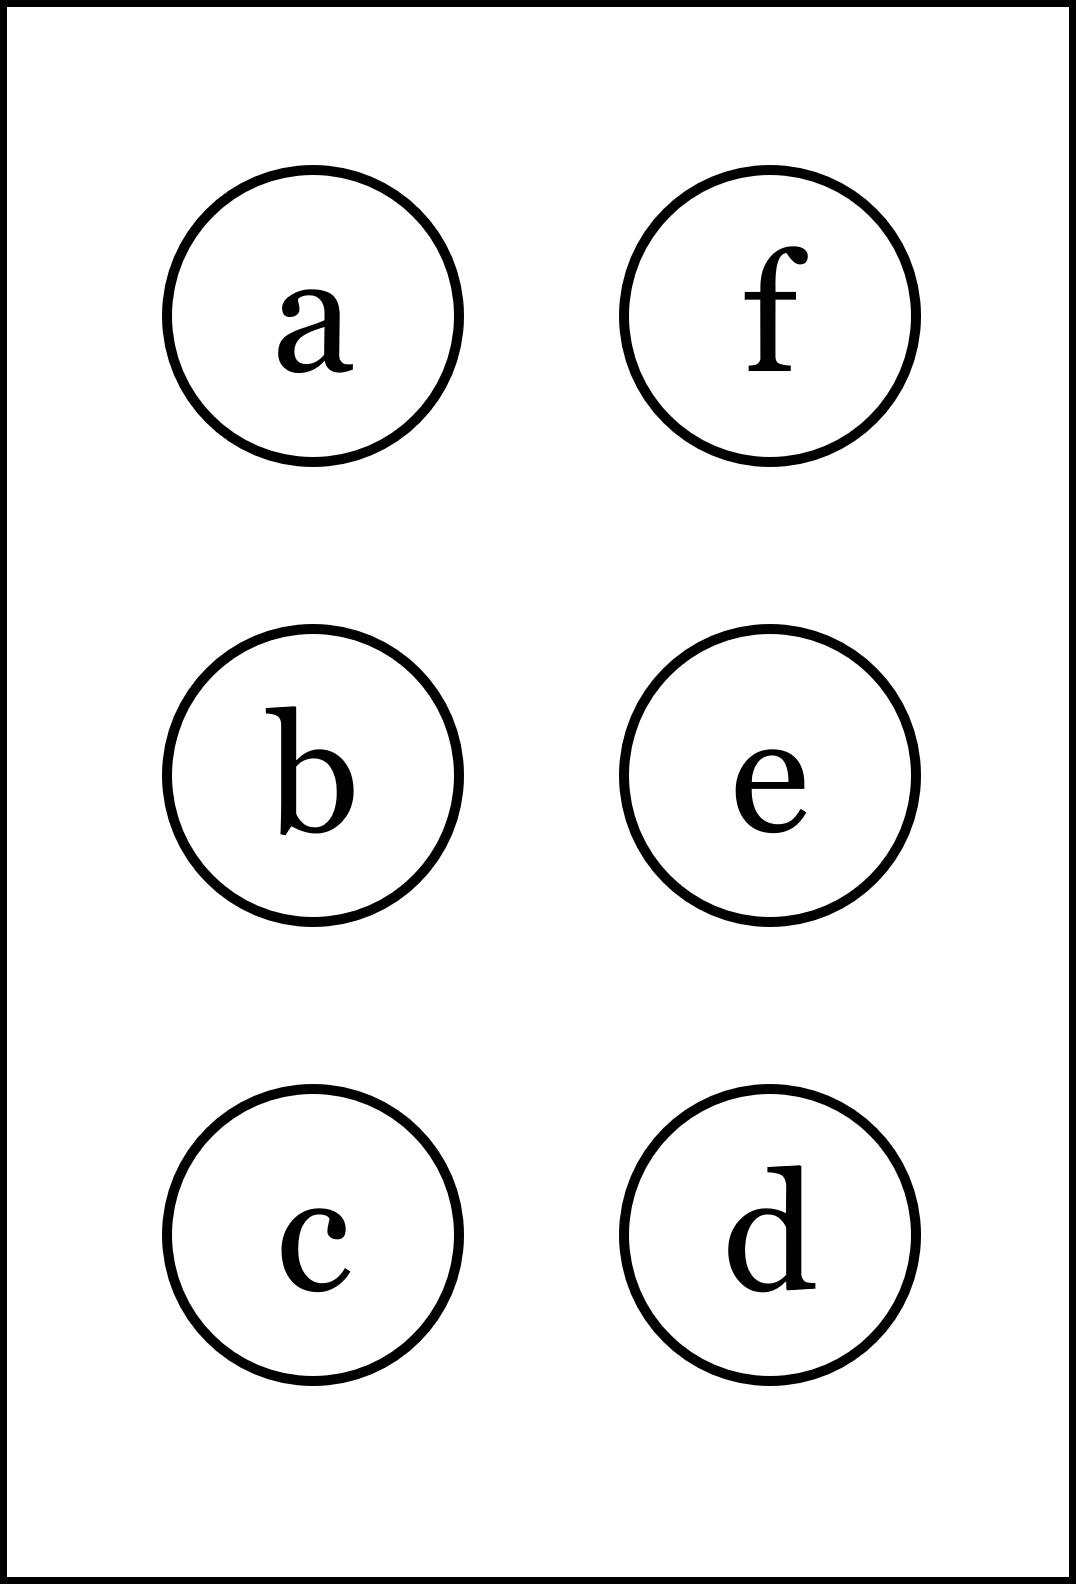
\includegraphics[height=40mm]{../images/braille.png}
{\small Písmeno Braillovej abecedy}
\end{center}
\end{minipage}
\end{center}
\end{minipage}
%
\end{tabular}
\newpage
\thispagestyle{empty}
\begin{tabular}{c:c}
\begin{minipage}[c][104.5mm][t]{0.5\linewidth}
\begin{center}
\vspace{7mm}
{\huge Definiční obor, skupina \textit{Mu $\mu$} -\romannumeral1}\\[5mm]
\textit{Jméno:}\phantom{xxxxxxxxxxxxxxxxxxxxxxxxxxxxxxxxxxxxxxxxxxxxxxxxxxxxxxxxxxxxxxxxx}\\[5mm]
\begin{minipage}{0.95\linewidth}
\begin{center}
\textbf{Zjisti definiční obor} zadaných funkcí. Pokud se shoduje s tím za otazníky,\\tak napravo obarvi příslušející kroužek načerno. \textbf{Spolu odevzdejte výsledné slovo}.
\end{center}
\end{minipage}
\\[1mm]
\begin{minipage}{0.79\linewidth}
\begin{center}
\begin{varwidth}{\linewidth}
\begin{enumerate}
\normalsizerrr
\item $f(x)=\cfrac{-x+5}{-x-8}$\quad \dotfill\; ???\;\dotfill \quad $\mathbb{R}\smallsetminus\{-8\}$
\item $f(x)=\cfrac{1}{-2x^3-16x^2-42x-36}$\quad \dotfill\; ???\;\dotfill \quad $\mathbb{R}\smallsetminus\{-3,-2\}$
\item $f(x)=\sqrt{2x+5}$\quad \dotfill\; ???\;\dotfill \quad $x\geq\nicefrac{-5}{2}$
\item $f(x)=\sqrt{-x^2+7x}$\quad \dotfill\; ???\;\dotfill \quad $x\in\langle0 , 7\rangle$
\item $f(x)=5\ln{(-9x-6)}$\quad \dotfill\; ???\;\dotfill \quad $x<\nicefrac{-2}{3}$
\item $f(x)=\ln{(x^2-9x+14)}$\quad \dotfill\; ???\;\dotfill \quad $x\in(2 , 7)$
\end{enumerate}
\end{varwidth}
\end{center}
\end{minipage}
\begin{minipage}{0.20\linewidth}
\begin{center}
{\Huge\bfseries 1.} \\[2mm]
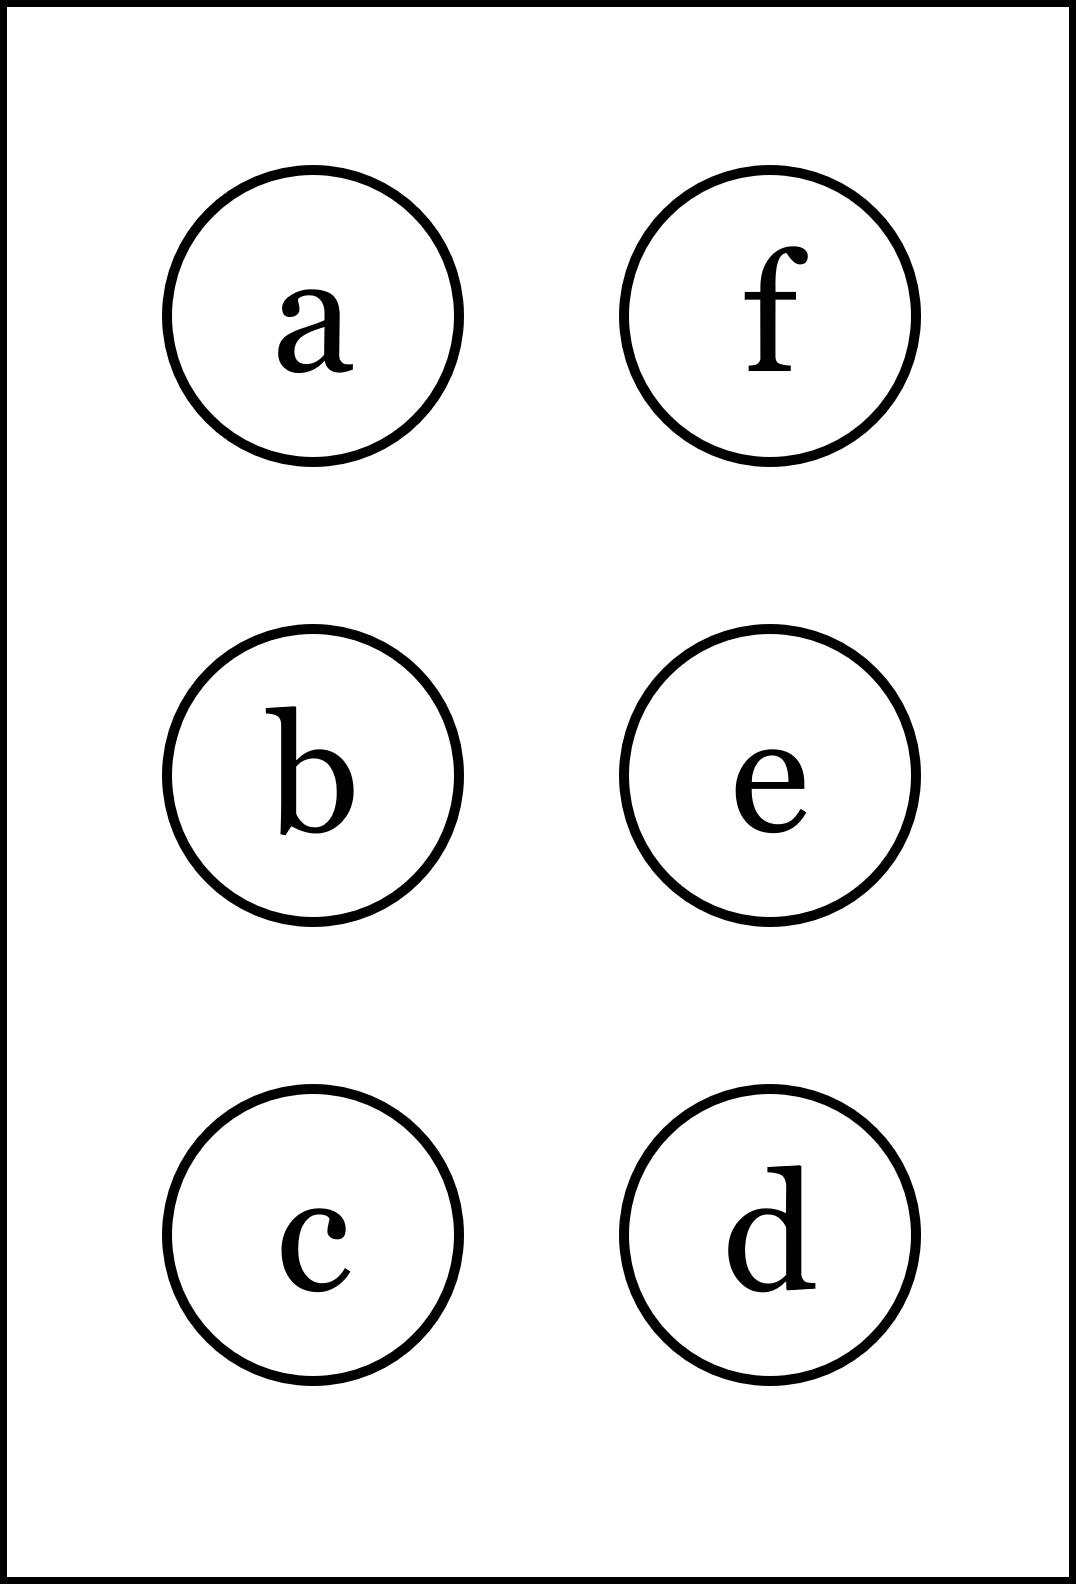
\includegraphics[height=40mm]{../images/braille.png}
{\small Písmeno Braillovej abecedy}
\end{center}
\end{minipage}
\end{center}
\end{minipage}
&
\begin{minipage}[c][104.5mm][t]{0.5\linewidth}
\begin{center}
\vspace{7mm}
{\huge Definiční obor, skupina \textit{Mu $\mu$} -\romannumeral2}\\[5mm]
\textit{Jméno:}\phantom{xxxxxxxxxxxxxxxxxxxxxxxxxxxxxxxxxxxxxxxxxxxxxxxxxxxxxxxxxxxxxxxxx}\\[5mm]
\begin{minipage}{0.95\linewidth}
\begin{center}
\textbf{Zjisti definiční obor} zadaných funkcí. Pokud se shoduje s tím za otazníky,\\tak napravo obarvi příslušející kroužek načerno. \textbf{Spolu odevzdejte výsledné slovo}.
\end{center}
\end{minipage}
\\[1mm]
\begin{minipage}{0.79\linewidth}
\begin{center}
\begin{varwidth}{\linewidth}
\begin{enumerate}
\normalsizerrr
\item $f(x)=\cfrac{x-7}{4x-2}$\quad \dotfill\; ???\;\dotfill \quad $\mathbb{R}\smallsetminus\{\nicefrac{-1}{2}\}$
\item $f(x)=\cfrac{1}{3x^3-3x^2-3x+3}$\quad \dotfill\; ???\;\dotfill \quad $\mathbb{R}\smallsetminus\{1,-1\}$
\item $f(x)=-5\sqrt{5x-5}$\quad \dotfill\; ???\;\dotfill \quad $x\leq1$
\item $f(x)=\sqrt{-x^2+3x}$\quad \dotfill\; ???\;\dotfill \quad $x\in(0 , 3)$
\item $f(x)=4\ln{(-5x+2)}$\quad \dotfill\; ???\;\dotfill \quad $x<\nicefrac{-2}{5}$
\item $f(x)=\ln{(x^2+3x-4)}$\quad \dotfill\; ???\;\dotfill \quad $x\in(-\infty , -4)\cup(1 , \infty)$
\end{enumerate}
\end{varwidth}
\end{center}
\end{minipage}
\begin{minipage}{0.20\linewidth}
\begin{center}
{\Huge\bfseries 2.} \\[2mm]
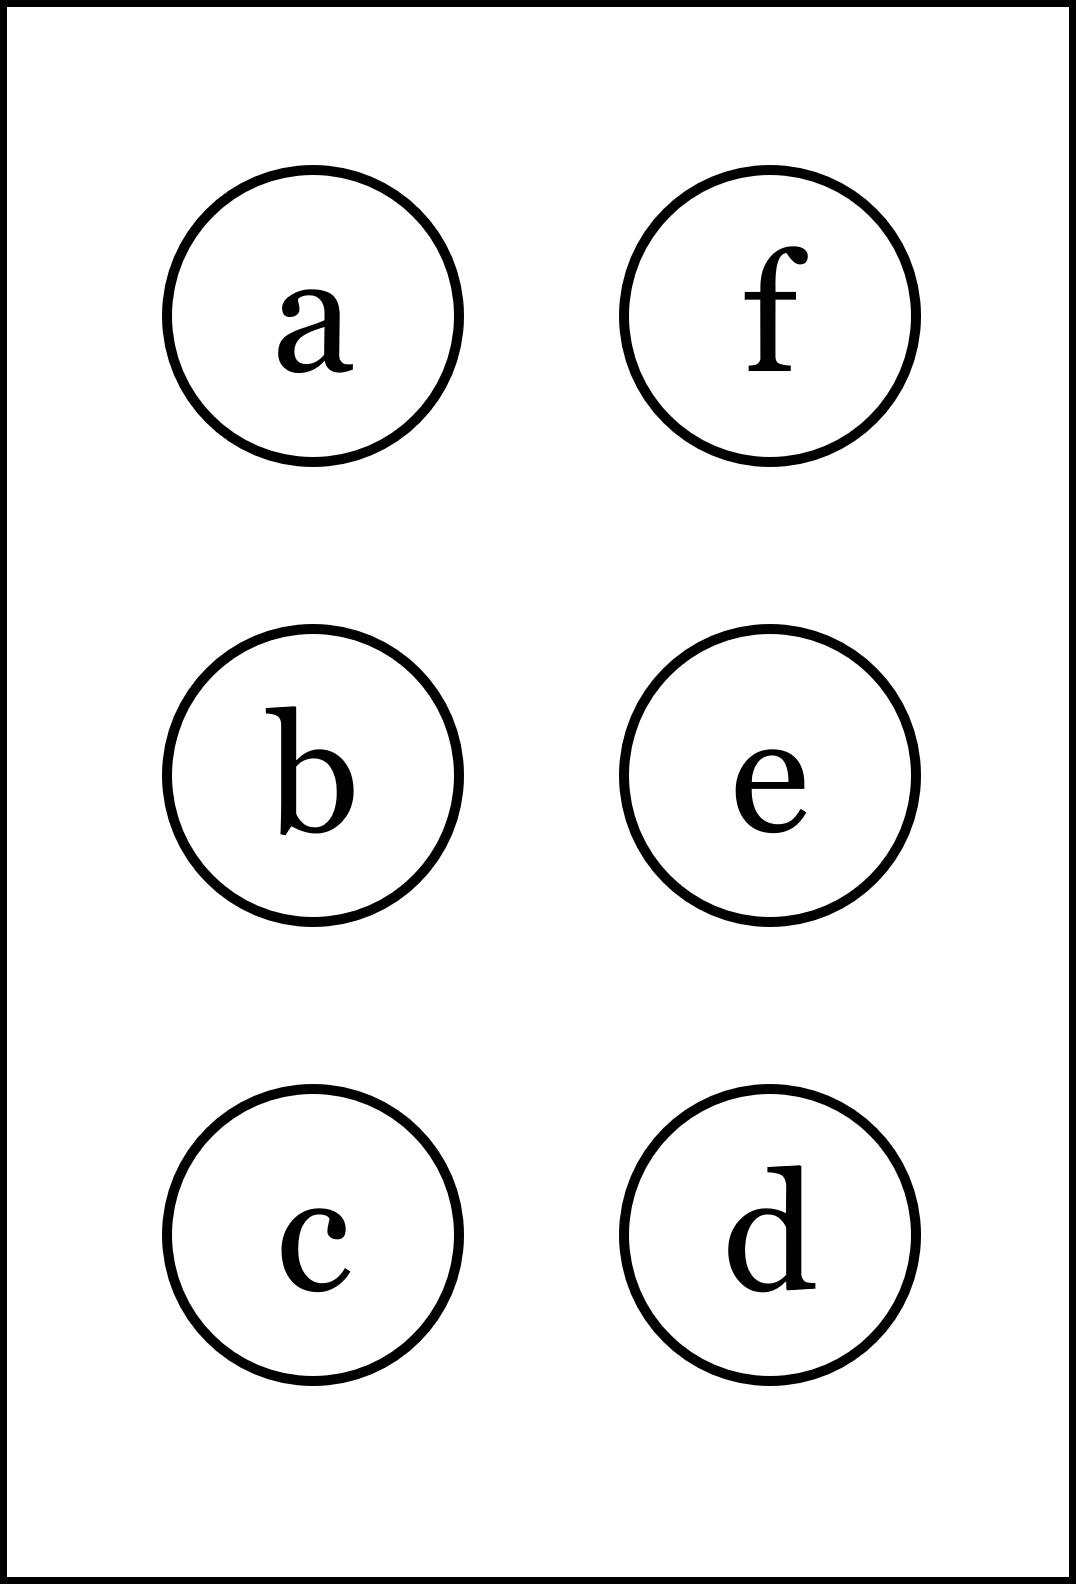
\includegraphics[height=40mm]{../images/braille.png}
{\small Písmeno Braillovej abecedy}
\end{center}
\end{minipage}
\end{center}
\end{minipage}
\\ \hdashline
\begin{minipage}[c][104.5mm][t]{0.5\linewidth}
\begin{center}
\vspace{7mm}
{\huge Definiční obor, skupina \textit{Mu $\mu$} -\romannumeral3}\\[5mm]
\textit{Jméno:}\phantom{xxxxxxxxxxxxxxxxxxxxxxxxxxxxxxxxxxxxxxxxxxxxxxxxxxxxxxxxxxxxxxxxx}\\[5mm]
\begin{minipage}{0.95\linewidth}
\begin{center}
\textbf{Zjisti definiční obor} zadaných funkcí. Pokud se shoduje s tím za otazníky,\\tak napravo obarvi příslušející kroužek načerno. \textbf{Spolu odevzdejte výsledné slovo}.
\end{center}
\end{minipage}
\\[1mm]
\begin{minipage}{0.79\linewidth}
\begin{center}
\begin{varwidth}{\linewidth}
\begin{enumerate}
\normalsizerrr
\item $f(x)=\cfrac{-7x-8}{5x+1}$\quad \dotfill\; ???\;\dotfill \quad $\mathbb{R}\smallsetminus\{\nicefrac{-1}{5}\}$
\item $f(x)=\cfrac{1}{2x^3+2x^2-10x+6}$\quad \dotfill\; ???\;\dotfill \quad $\mathbb{R}\smallsetminus\{1,-3\}$
\item $f(x)=\sqrt{-2x-7}$\quad \dotfill\; ???\;\dotfill \quad $x\leq\nicefrac{7}{2}$
\item $f(x)=\sqrt{-x^2+7x}$\quad \dotfill\; ???\;\dotfill \quad $x\in\langle-7 , 0\rangle$
\item $f(x)=\ln{(2x-2)}$\quad \dotfill\; ???\;\dotfill \quad $x<1$
\item $f(x)=\ln{(x^2-14x+49)}$\quad \dotfill\; ???\;\dotfill \quad $x\in(-\infty , 7)\cup(7 , \infty)$
\end{enumerate}
\end{varwidth}
\end{center}
\end{minipage}
\begin{minipage}{0.20\linewidth}
\begin{center}
{\Huge\bfseries 3.} \\[2mm]
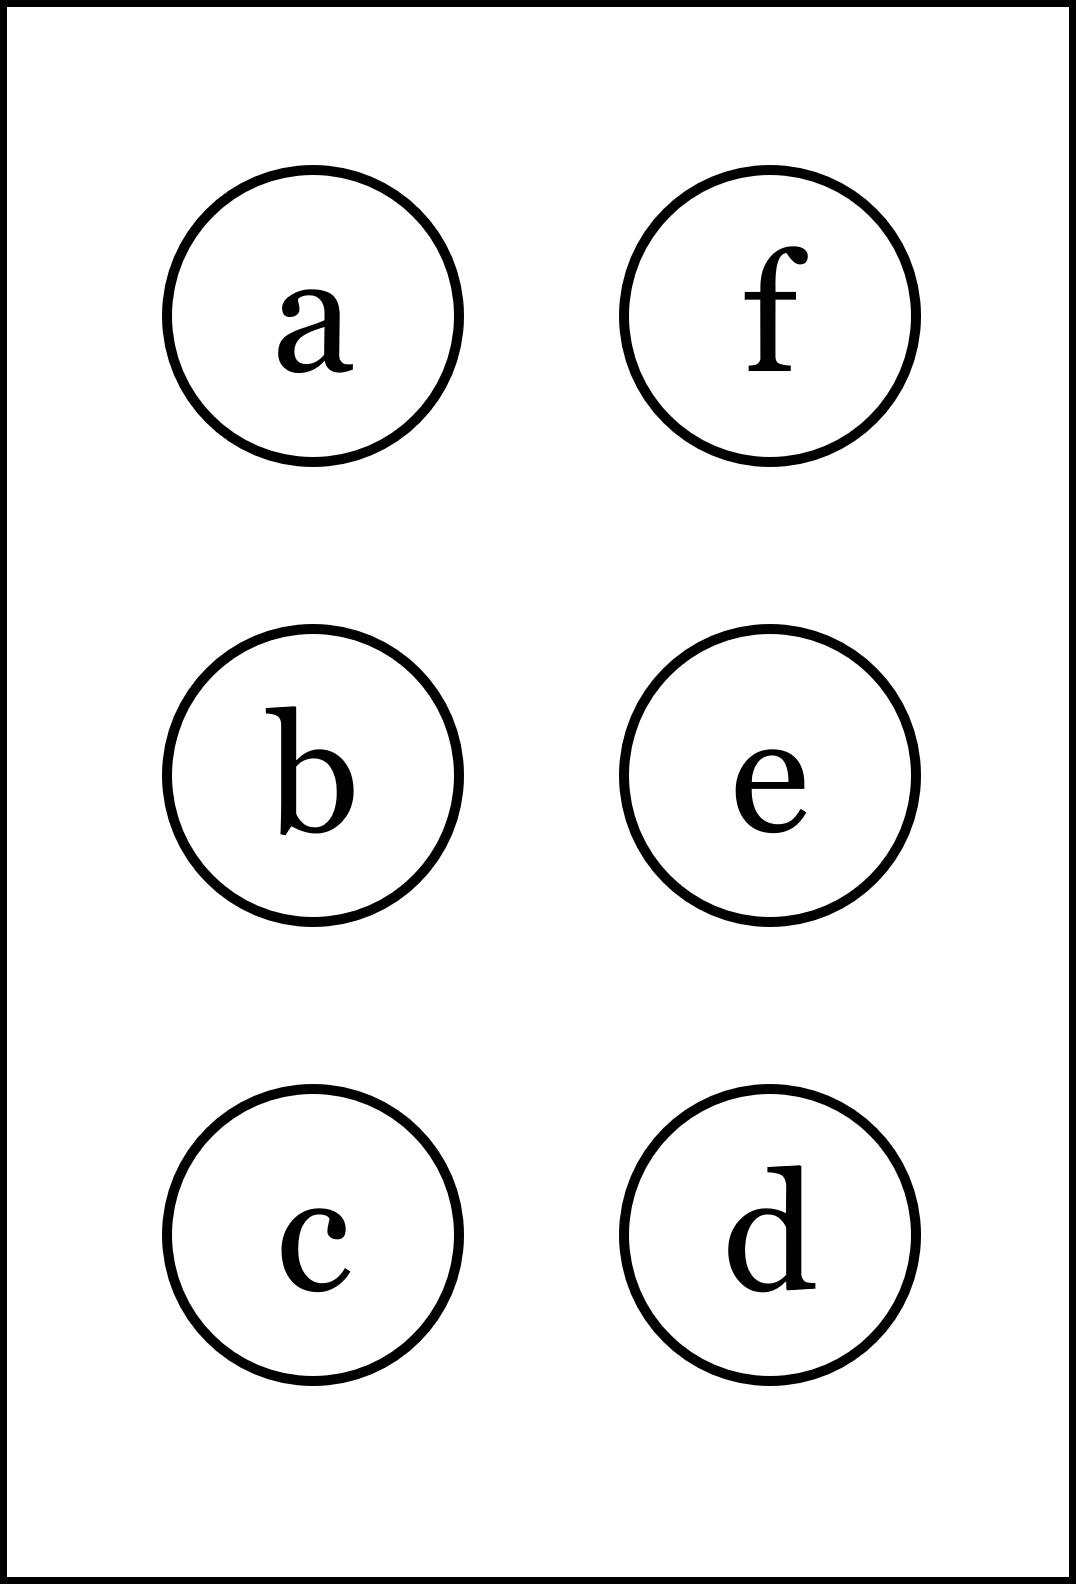
\includegraphics[height=40mm]{../images/braille.png}
{\small Písmeno Braillovej abecedy}
\end{center}
\end{minipage}
\end{center}
\end{minipage}
&
\begin{minipage}[c][104.5mm][t]{0.5\linewidth}
\begin{center}
\vspace{7mm}
{\huge Definiční obor, skupina \textit{Mu $\mu$} -\romannumeral4}\\[5mm]
\textit{Jméno:}\phantom{xxxxxxxxxxxxxxxxxxxxxxxxxxxxxxxxxxxxxxxxxxxxxxxxxxxxxxxxxxxxxxxxx}\\[5mm]
\begin{minipage}{0.95\linewidth}
\begin{center}
\textbf{Zjisti definiční obor} zadaných funkcí. Pokud se shoduje s tím za otazníky,\\tak napravo obarvi příslušející kroužek načerno. \textbf{Spolu odevzdejte výsledné slovo}.
\end{center}
\end{minipage}
\\[1mm]
\begin{minipage}{0.79\linewidth}
\begin{center}
\begin{varwidth}{\linewidth}
\begin{enumerate}
\normalsizerrr
\item $f(x)=\cfrac{9x-9}{-3x+2}$\quad \dotfill\; ???\;\dotfill \quad $\mathbb{R}\smallsetminus\{\nicefrac{-2}{3}\}$
\item $f(x)=\cfrac{1}{x^3-4x^2-20x+48}$\quad \dotfill\; ???\;\dotfill \quad $\mathbb{R}\smallsetminus\{2,-4,6\}$
\item $f(x)=-6\sqrt{2x+3}$\quad \dotfill\; ???\;\dotfill \quad $x\geq\nicefrac{3}{2}$
\item $f(x)=\sqrt{-x^2+8x}$\quad \dotfill\; ???\;\dotfill \quad $x\in\langle-8 , 0\rangle$
\item $f(x)=6\ln{(-7x-3)}$\quad \dotfill\; ???\;\dotfill \quad $x>\nicefrac{-3}{7}$
\item $f(x)=\ln{(x^2-10x+21)}$\quad \dotfill\; ???\;\dotfill \quad $x\in(-\infty , 3)\cup(7 , \infty)$
\end{enumerate}
\end{varwidth}
\end{center}
\end{minipage}
\begin{minipage}{0.20\linewidth}
\begin{center}
{\Huge\bfseries 4.} \\[2mm]
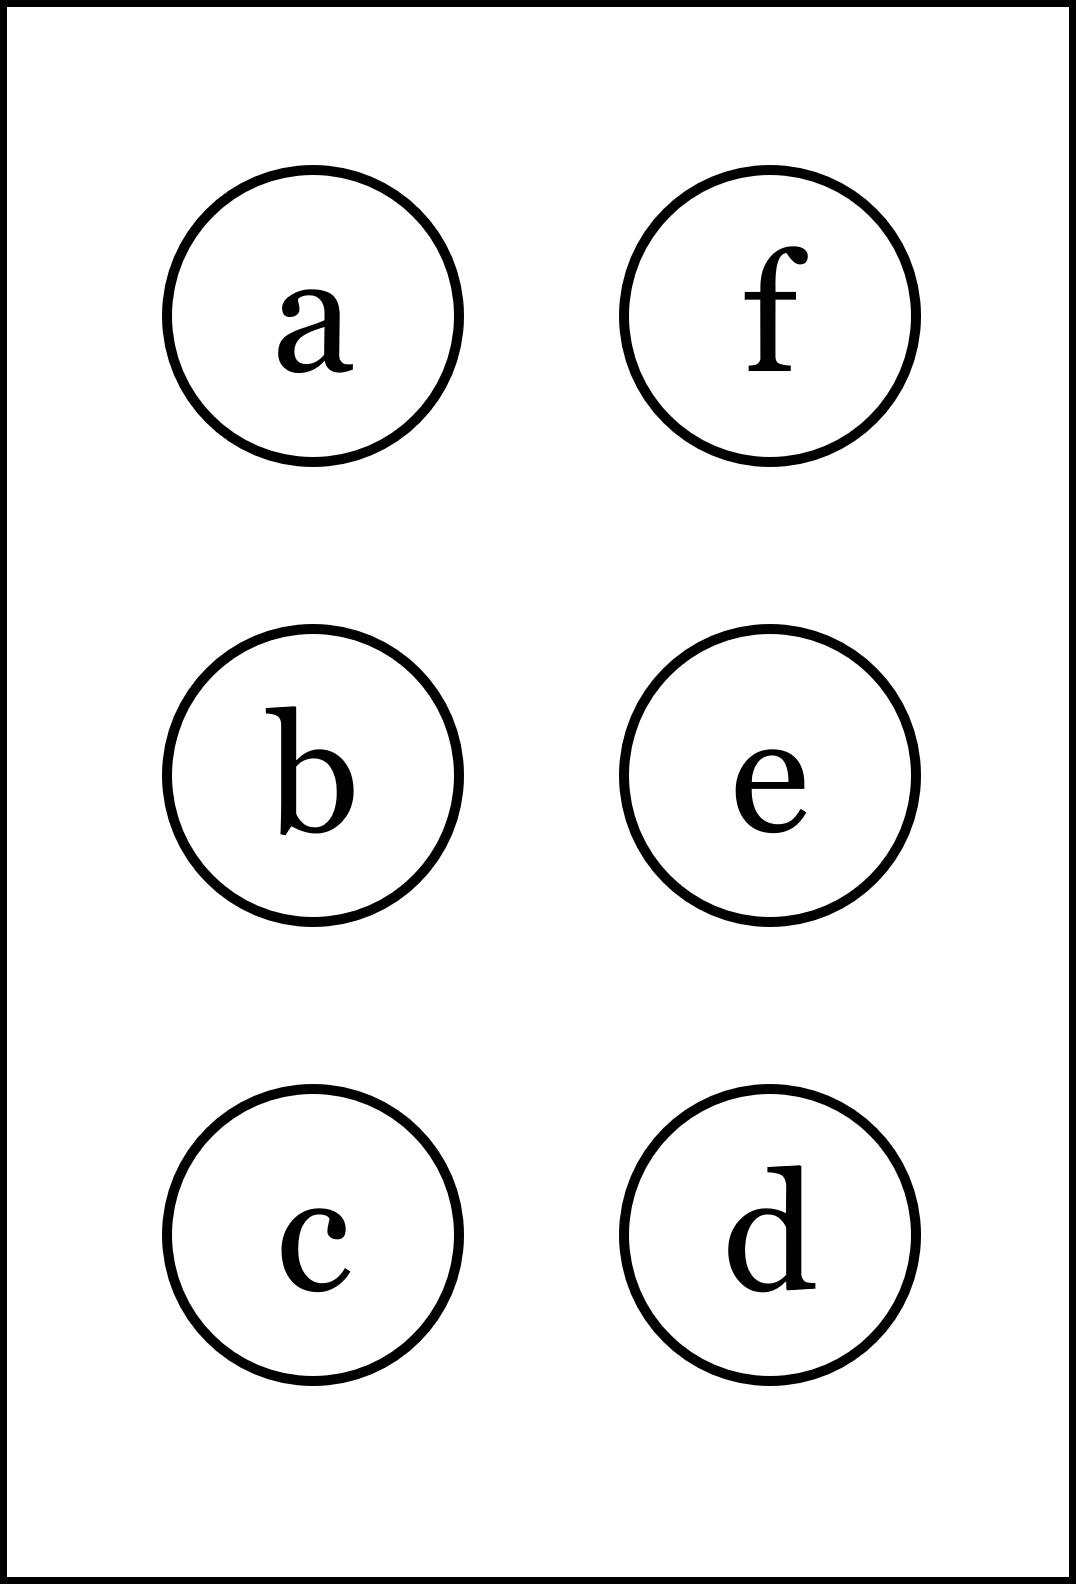
\includegraphics[height=40mm]{../images/braille.png}
{\small Písmeno Braillovej abecedy}
\end{center}
\end{minipage}
\end{center}
\end{minipage}
%
\end{tabular}
\newpage
\thispagestyle{empty}
\begin{tabular}{c:c}
\begin{minipage}[c][104.5mm][t]{0.5\linewidth}
\begin{center}
\vspace{7mm}
{\huge Definiční obor, skupina \textit{Nu $\nu$} -\romannumeral1}\\[5mm]
\textit{Jméno:}\phantom{xxxxxxxxxxxxxxxxxxxxxxxxxxxxxxxxxxxxxxxxxxxxxxxxxxxxxxxxxxxxxxxxx}\\[5mm]
\begin{minipage}{0.95\linewidth}
\begin{center}
\textbf{Zjisti definiční obor} zadaných funkcí. Pokud se shoduje s tím za otazníky,\\tak napravo obarvi příslušející kroužek načerno. \textbf{Spolu odevzdejte výsledné slovo}.
\end{center}
\end{minipage}
\\[1mm]
\begin{minipage}{0.79\linewidth}
\begin{center}
\begin{varwidth}{\linewidth}
\begin{enumerate}
\normalsizerrr
\item $f(x)=\cfrac{-6x-1}{-7x+9}$\quad \dotfill\; ???\;\dotfill \quad $\mathbb{R}\smallsetminus\{\nicefrac{9}{7}\}$
\item $f(x)=\cfrac{1}{-3x^3-18x^2-9x+30}$\quad \dotfill\; ???\;\dotfill \quad $\mathbb{R}\smallsetminus\{1,-4,5\}$
\item $f(x)=4\sqrt{2x-8}$\quad \dotfill\; ???\;\dotfill \quad $x\leq4$
\item $f(x)=\sqrt{-x^2-2x}$\quad \dotfill\; ???\;\dotfill \quad $x\in\langle-2 , 0\rangle$
\item $f(x)=2\ln{(8x-4)}$\quad \dotfill\; ???\;\dotfill \quad $x>\nicefrac{-1}{2}$
\item $f(x)=\ln{(x^2+4x-5)}$\quad \dotfill\; ???\;\dotfill \quad $x\in(-\infty , -5)\cup(1 , \infty)$
\end{enumerate}
\end{varwidth}
\end{center}
\end{minipage}
\begin{minipage}{0.20\linewidth}
\begin{center}
{\Huge\bfseries 1.} \\[2mm]
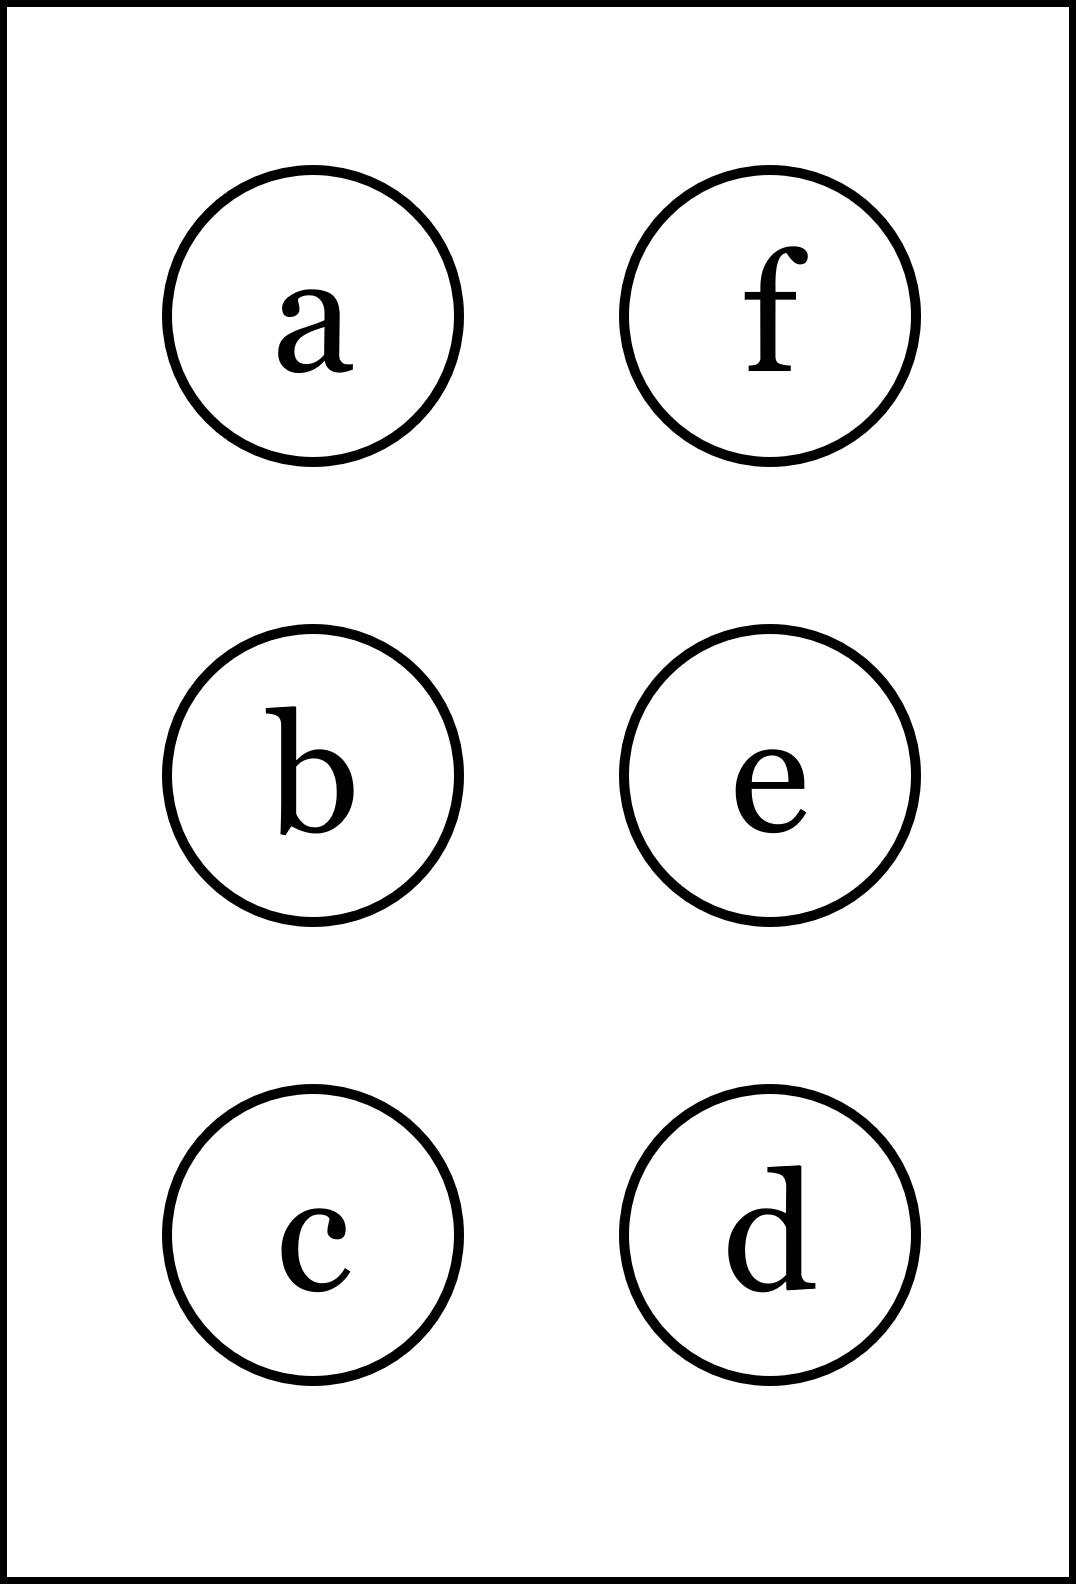
\includegraphics[height=40mm]{../images/braille.png}
{\small Písmeno Braillovej abecedy}
\end{center}
\end{minipage}
\end{center}
\end{minipage}
&
\begin{minipage}[c][104.5mm][t]{0.5\linewidth}
\begin{center}
\vspace{7mm}
{\huge Definiční obor, skupina \textit{Nu $\nu$} -\romannumeral2}\\[5mm]
\textit{Jméno:}\phantom{xxxxxxxxxxxxxxxxxxxxxxxxxxxxxxxxxxxxxxxxxxxxxxxxxxxxxxxxxxxxxxxxx}\\[5mm]
\begin{minipage}{0.95\linewidth}
\begin{center}
\textbf{Zjisti definiční obor} zadaných funkcí. Pokud se shoduje s tím za otazníky,\\tak napravo obarvi příslušející kroužek načerno. \textbf{Spolu odevzdejte výsledné slovo}.
\end{center}
\end{minipage}
\\[1mm]
\begin{minipage}{0.79\linewidth}
\begin{center}
\begin{varwidth}{\linewidth}
\begin{enumerate}
\normalsizerrr
\item $f(x)=\cfrac{2x-5}{-2x+6}$\quad \dotfill\; ???\;\dotfill \quad $\mathbb{R}\smallsetminus\{3\}$
\item $f(x)=\cfrac{1}{-2x^3+4x^2+2x-4}$\quad \dotfill\; ???\;\dotfill \quad $\mathbb{R}\smallsetminus\{4,-1\}$
\item $f(x)=4\sqrt{7x+1}$\quad \dotfill\; ???\;\dotfill \quad $x\geq\nicefrac{-1}{7}$
\item $f(x)=\sqrt{-x^2+8x}$\quad \dotfill\; ???\;\dotfill \quad $x\in\langle-8 , 0\rangle$
\item $f(x)=-6\ln{(2x-5)}$\quad \dotfill\; ???\;\dotfill \quad $x>\nicefrac{5}{2}$
\item $f(x)=\ln{(x^2+2x+1)}$\quad \dotfill\; ???\;\dotfill \quad $x\in(-1 , -1)$
\end{enumerate}
\end{varwidth}
\end{center}
\end{minipage}
\begin{minipage}{0.20\linewidth}
\begin{center}
{\Huge\bfseries 2.} \\[2mm]
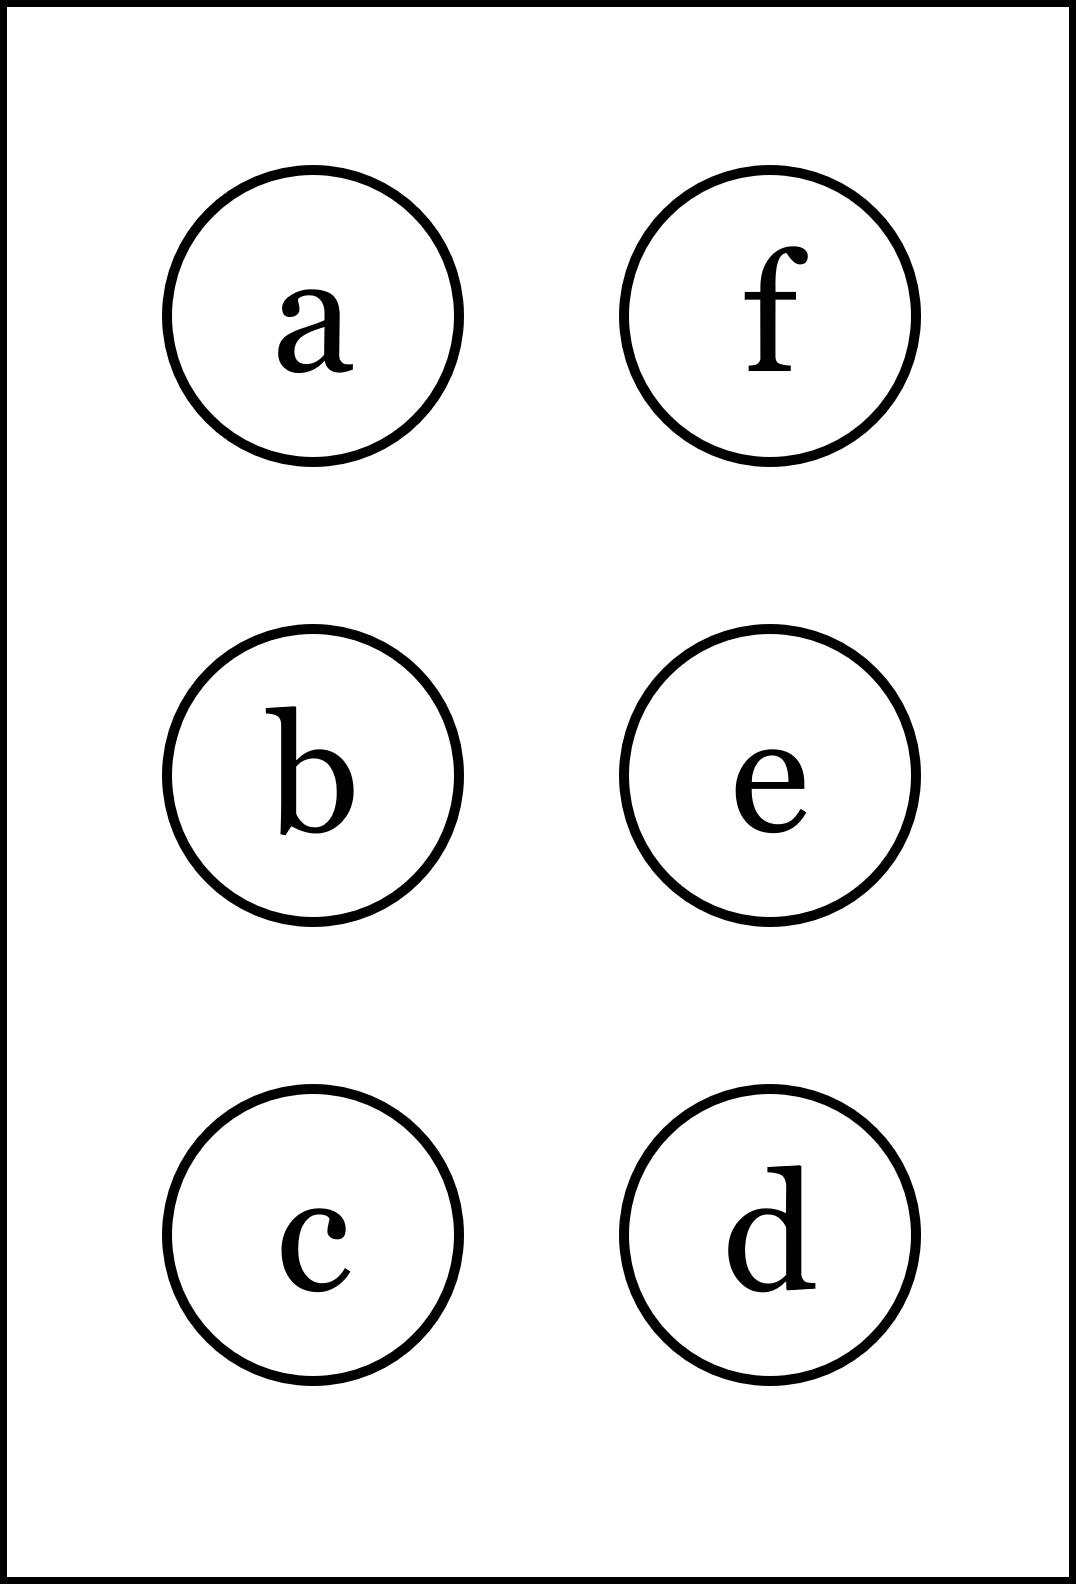
\includegraphics[height=40mm]{../images/braille.png}
{\small Písmeno Braillovej abecedy}
\end{center}
\end{minipage}
\end{center}
\end{minipage}
\\ \hdashline
\begin{minipage}[c][104.5mm][t]{0.5\linewidth}
\begin{center}
\vspace{7mm}
{\huge Definiční obor, skupina \textit{Nu $\nu$} -\romannumeral3}\\[5mm]
\textit{Jméno:}\phantom{xxxxxxxxxxxxxxxxxxxxxxxxxxxxxxxxxxxxxxxxxxxxxxxxxxxxxxxxxxxxxxxxx}\\[5mm]
\begin{minipage}{0.95\linewidth}
\begin{center}
\textbf{Zjisti definiční obor} zadaných funkcí. Pokud se shoduje s tím za otazníky,\\tak napravo obarvi příslušející kroužek načerno. \textbf{Spolu odevzdejte výsledné slovo}.
\end{center}
\end{minipage}
\\[1mm]
\begin{minipage}{0.79\linewidth}
\begin{center}
\begin{varwidth}{\linewidth}
\begin{enumerate}
\normalsizerrr
\item $f(x)=\cfrac{x+6}{8x-4}$\quad \dotfill\; ???\;\dotfill \quad $\mathbb{R}\smallsetminus\{\nicefrac{1}{2}\}$
\item $f(x)=\cfrac{1}{6x^3-18x-12}$\quad \dotfill\; ???\;\dotfill \quad $\mathbb{R}\smallsetminus\{1,2,-2\}$
\item $f(x)=8\sqrt{7x-3}$\quad \dotfill\; ???\;\dotfill \quad $x\geq\nicefrac{3}{7}$
\item $f(x)=\sqrt{-x^2+5x}$\quad \dotfill\; ???\;\dotfill \quad $x\in\langle-5 , 0\rangle$
\item $f(x)=\ln{(-7x-6)}$\quad \dotfill\; ???\;\dotfill \quad $x>\nicefrac{-6}{7}$
\item $f(x)=\ln{(x^2+7x+12)}$\quad \dotfill\; ???\;\dotfill \quad $x\in(-4 , -3)$
\end{enumerate}
\end{varwidth}
\end{center}
\end{minipage}
\begin{minipage}{0.20\linewidth}
\begin{center}
{\Huge\bfseries 3.} \\[2mm]
\includegraphics[height=40mm]{../images/braille.png}
{\small Písmeno Braillovej abecedy}
\end{center}
\end{minipage}
\end{center}
\end{minipage}
&
\begin{minipage}[c][104.5mm][t]{0.5\linewidth}
\begin{center}
\vspace{7mm}
{\huge Definiční obor, skupina \textit{Nu $\nu$} -\romannumeral4}\\[5mm]
\textit{Jméno:}\phantom{xxxxxxxxxxxxxxxxxxxxxxxxxxxxxxxxxxxxxxxxxxxxxxxxxxxxxxxxxxxxxxxxx}\\[5mm]
\begin{minipage}{0.95\linewidth}
\begin{center}
\textbf{Zjisti definiční obor} zadaných funkcí. Pokud se shoduje s tím za otazníky,\\tak napravo obarvi příslušející kroužek načerno. \textbf{Spolu odevzdejte výsledné slovo}.
\end{center}
\end{minipage}
\\[1mm]
\begin{minipage}{0.79\linewidth}
\begin{center}
\begin{varwidth}{\linewidth}
\begin{enumerate}
\normalsizerrr
\item $f(x)=\cfrac{-x+2}{-x-3}$\quad \dotfill\; ???\;\dotfill \quad $\mathbb{R}\smallsetminus\{-3\}$
\item $f(x)=\cfrac{1}{-5x^3-25x^2+5x+25}$\quad \dotfill\; ???\;\dotfill \quad $\mathbb{R}\smallsetminus\{1,-5,-1\}$
\item $f(x)=-7\sqrt{-6x+3}$\quad \dotfill\; ???\;\dotfill \quad $x\leq\nicefrac{1}{2}$
\item $f(x)=\sqrt{-x^2-x}$\quad \dotfill\; ???\;\dotfill \quad $x\in(-1 , 0)$
\item $f(x)=-\ln{(x+4)}$\quad \dotfill\; ???\;\dotfill \quad $x>4$
\item $f(x)=\ln{(x^2+5x+4)}$\quad \dotfill\; ???\;\dotfill \quad $x\in(-4 , -1)$
\end{enumerate}
\end{varwidth}
\end{center}
\end{minipage}
\begin{minipage}{0.20\linewidth}
\begin{center}
{\Huge\bfseries 4.} \\[2mm]
\includegraphics[height=40mm]{../images/braille.png}
{\small Písmeno Braillovej abecedy}
\end{center}
\end{minipage}
\end{center}
\end{minipage}
%
\end{tabular}
\newpage
\thispagestyle{empty}
\begin{tabular}{c:c}
\begin{minipage}[c][104.5mm][t]{0.5\linewidth}
\begin{center}
\vspace{7mm}
{\huge Definiční obor, skupina \textit{Xi $\xi$} -\romannumeral1}\\[5mm]
\textit{Jméno:}\phantom{xxxxxxxxxxxxxxxxxxxxxxxxxxxxxxxxxxxxxxxxxxxxxxxxxxxxxxxxxxxxxxxxx}\\[5mm]
\begin{minipage}{0.95\linewidth}
\begin{center}
\textbf{Zjisti definiční obor} zadaných funkcí. Pokud se shoduje s tím za otazníky,\\tak napravo obarvi příslušející kroužek načerno. \textbf{Spolu odevzdejte výsledné slovo}.
\end{center}
\end{minipage}
\\[1mm]
\begin{minipage}{0.79\linewidth}
\begin{center}
\begin{varwidth}{\linewidth}
\begin{enumerate}
\normalsizerrr
\item $f(x)=\cfrac{x+2}{-x+6}$\quad \dotfill\; ???\;\dotfill \quad $\mathbb{R}\smallsetminus\{6\}$
\item $f(x)=\cfrac{1}{-3x^3+9x+6}$\quad \dotfill\; ???\;\dotfill \quad $\mathbb{R}\smallsetminus\{0,1,2\}$
\item $f(x)=-\sqrt{-5x+2}$\quad \dotfill\; ???\;\dotfill \quad $x\leq\nicefrac{-2}{5}$
\item $f(x)=\sqrt{-x^2-6x}$\quad \dotfill\; ???\;\dotfill \quad $x\in(-6 , 0)$
\item $f(x)=2\ln{(-4x-3)}$\quad \dotfill\; ???\;\dotfill \quad $x<\nicefrac{-3}{4}$
\item $f(x)=\ln{(x^2-2x-3)}$\quad \dotfill\; ???\;\dotfill \quad $x\in(-\infty , -1)\cup(3 , \infty)$
\end{enumerate}
\end{varwidth}
\end{center}
\end{minipage}
\begin{minipage}{0.20\linewidth}
\begin{center}
{\Huge\bfseries 1.} \\[2mm]
\includegraphics[height=40mm]{../images/braille.png}
{\small Písmeno Braillovej abecedy}
\end{center}
\end{minipage}
\end{center}
\end{minipage}
&
\begin{minipage}[c][104.5mm][t]{0.5\linewidth}
\begin{center}
\vspace{7mm}
{\huge Definiční obor, skupina \textit{Xi $\xi$} -\romannumeral2}\\[5mm]
\textit{Jméno:}\phantom{xxxxxxxxxxxxxxxxxxxxxxxxxxxxxxxxxxxxxxxxxxxxxxxxxxxxxxxxxxxxxxxxx}\\[5mm]
\begin{minipage}{0.95\linewidth}
\begin{center}
\textbf{Zjisti definiční obor} zadaných funkcí. Pokud se shoduje s tím za otazníky,\\tak napravo obarvi příslušející kroužek načerno. \textbf{Spolu odevzdejte výsledné slovo}.
\end{center}
\end{minipage}
\\[1mm]
\begin{minipage}{0.79\linewidth}
\begin{center}
\begin{varwidth}{\linewidth}
\begin{enumerate}
\normalsizerrr
\item $f(x)=\cfrac{6x+5}{-6x+8}$\quad \dotfill\; ???\;\dotfill \quad $\mathbb{R}\smallsetminus\{\nicefrac{4}{3}\}$
\item $f(x)=\cfrac{1}{-4x^3-8x^2+20x+24}$\quad \dotfill\; ???\;\dotfill \quad $\mathbb{R}\smallsetminus\{2,-3,-1\}$
\item $f(x)=-8\sqrt{-x+6}$\quad \dotfill\; ???\;\dotfill \quad $x\leq6$
\item $f(x)=\sqrt{-x^2+x}$\quad \dotfill\; ???\;\dotfill \quad $x\in(0 , 1)$
\item $f(x)=9\ln{(-2x-1)}$\quad \dotfill\; ???\;\dotfill \quad $x<\nicefrac{-1}{2}$
\item $f(x)=\ln{(x^2-7x+6)}$\quad \dotfill\; ???\;\dotfill \quad $x\in(1 , 6)$
\end{enumerate}
\end{varwidth}
\end{center}
\end{minipage}
\begin{minipage}{0.20\linewidth}
\begin{center}
{\Huge\bfseries 2.} \\[2mm]
\includegraphics[height=40mm]{../images/braille.png}
{\small Písmeno Braillovej abecedy}
\end{center}
\end{minipage}
\end{center}
\end{minipage}
\\ \hdashline
\begin{minipage}[c][104.5mm][t]{0.5\linewidth}
\begin{center}
\vspace{7mm}
{\huge Definiční obor, skupina \textit{Xi $\xi$} -\romannumeral3}\\[5mm]
\textit{Jméno:}\phantom{xxxxxxxxxxxxxxxxxxxxxxxxxxxxxxxxxxxxxxxxxxxxxxxxxxxxxxxxxxxxxxxxx}\\[5mm]
\begin{minipage}{0.95\linewidth}
\begin{center}
\textbf{Zjisti definiční obor} zadaných funkcí. Pokud se shoduje s tím za otazníky,\\tak napravo obarvi příslušející kroužek načerno. \textbf{Spolu odevzdejte výsledné slovo}.
\end{center}
\end{minipage}
\\[1mm]
\begin{minipage}{0.79\linewidth}
\begin{center}
\begin{varwidth}{\linewidth}
\begin{enumerate}
\normalsizerrr
\item $f(x)=\cfrac{-7x-1}{5x+5}$\quad \dotfill\; ???\;\dotfill \quad $\mathbb{R}\smallsetminus\{-1\}$
\item $f(x)=\cfrac{1}{x^3-4x^2-19x-14}$\quad \dotfill\; ???\;\dotfill \quad $\mathbb{R}\smallsetminus\{1,-2,6\}$
\item $f(x)=3\sqrt{8x+9}$\quad \dotfill\; ???\;\dotfill \quad $x\geq\nicefrac{9}{8}$
\item $f(x)=\sqrt{-x^2+3x}$\quad \dotfill\; ???\;\dotfill \quad $x\in(0 , 3)$
\item $f(x)=-3\ln{(2x-9)}$\quad \dotfill\; ???\;\dotfill \quad $x>\nicefrac{-9}{2}$
\item $f(x)=\ln{(x^2+6x-7)}$\quad \dotfill\; ???\;\dotfill \quad $x\in(-7 , 1)$
\end{enumerate}
\end{varwidth}
\end{center}
\end{minipage}
\begin{minipage}{0.20\linewidth}
\begin{center}
{\Huge\bfseries 3.} \\[2mm]
\includegraphics[height=40mm]{../images/braille.png}
{\small Písmeno Braillovej abecedy}
\end{center}
\end{minipage}
\end{center}
\end{minipage}
&
\begin{minipage}[c][104.5mm][t]{0.5\linewidth}
\begin{center}
\vspace{7mm}
{\huge Definiční obor, skupina \textit{Xi $\xi$} -\romannumeral4}\\[5mm]
\textit{Jméno:}\phantom{xxxxxxxxxxxxxxxxxxxxxxxxxxxxxxxxxxxxxxxxxxxxxxxxxxxxxxxxxxxxxxxxx}\\[5mm]
\begin{minipage}{0.95\linewidth}
\begin{center}
\textbf{Zjisti definiční obor} zadaných funkcí. Pokud se shoduje s tím za otazníky,\\tak napravo obarvi příslušející kroužek načerno. \textbf{Spolu odevzdejte výsledné slovo}.
\end{center}
\end{minipage}
\\[1mm]
\begin{minipage}{0.79\linewidth}
\begin{center}
\begin{varwidth}{\linewidth}
\begin{enumerate}
\normalsizerrr
\item $f(x)=\cfrac{-x-1}{4x+1}$\quad \dotfill\; ???\;\dotfill \quad $\mathbb{R}\smallsetminus\{\nicefrac{-1}{4}\}$
\item $f(x)=\cfrac{1}{-4x^3-28x^2-56x-32}$\quad \dotfill\; ???\;\dotfill \quad $\mathbb{R}\smallsetminus\{1,-6,-2\}$
\item $f(x)=2\sqrt{x+3}$\quad \dotfill\; ???\;\dotfill \quad $x\geq-3$
\item $f(x)=\sqrt{-x^2-3x}$\quad \dotfill\; ???\;\dotfill \quad $x\in\langle0 , 3\rangle$
\item $f(x)=3\ln{(8x-6)}$\quad \dotfill\; ???\;\dotfill \quad $x>\nicefrac{-3}{4}$
\item $f(x)=\ln{(x^2-8x+16)}$\quad \dotfill\; ???\;\dotfill \quad $x\in(4 , 4)$
\end{enumerate}
\end{varwidth}
\end{center}
\end{minipage}
\begin{minipage}{0.20\linewidth}
\begin{center}
{\Huge\bfseries 4.} \\[2mm]
\includegraphics[height=40mm]{../images/braille.png}
{\small Písmeno Braillovej abecedy}
\end{center}
\end{minipage}
\end{center}
\end{minipage}
%
\end{tabular}
\newpage
\thispagestyle{empty}
\begin{tabular}{c:c}
\begin{minipage}[c][104.5mm][t]{0.5\linewidth}
\begin{center}
\vspace{7mm}
{\huge Definiční obor, skupina \textit{Omicron $\omicron$} -\romannumeral1}\\[5mm]
\textit{Jméno:}\phantom{xxxxxxxxxxxxxxxxxxxxxxxxxxxxxxxxxxxxxxxxxxxxxxxxxxxxxxxxxxxxxxxxx}\\[5mm]
\begin{minipage}{0.95\linewidth}
\begin{center}
\textbf{Zjisti definiční obor} zadaných funkcí. Pokud se shoduje s tím za otazníky,\\tak napravo obarvi příslušející kroužek načerno. \textbf{Spolu odevzdejte výsledné slovo}.
\end{center}
\end{minipage}
\\[1mm]
\begin{minipage}{0.79\linewidth}
\begin{center}
\begin{varwidth}{\linewidth}
\begin{enumerate}
\normalsizerrr
\item $f(x)=\cfrac{x+4}{-3x-5}$\quad \dotfill\; ???\;\dotfill \quad $\mathbb{R}\smallsetminus\{\nicefrac{-5}{3}\}$
\item $f(x)=\cfrac{1}{-x^3-2x^2+13x-10}$\quad \dotfill\; ???\;\dotfill \quad $\mathbb{R}\smallsetminus\{1,5\}$
\item $f(x)=3\sqrt{5x+7}$\quad \dotfill\; ???\;\dotfill \quad $x\geq\nicefrac{7}{5}$
\item $f(x)=\sqrt{-x^2+3x}$\quad \dotfill\; ???\;\dotfill \quad $x\in\langle-3 , 0\rangle$
\item $f(x)=-4\ln{(-4x-7)}$\quad \dotfill\; ???\;\dotfill \quad $x<\nicefrac{7}{4}$
\item $f(x)=\ln{(x^2-2x-35)}$\quad \dotfill\; ???\;\dotfill \quad $x\in(-5 , 7)$
\end{enumerate}
\end{varwidth}
\end{center}
\end{minipage}
\begin{minipage}{0.20\linewidth}
\begin{center}
{\Huge\bfseries 1.} \\[2mm]
\includegraphics[height=40mm]{../images/braille.png}
{\small Písmeno Braillovej abecedy}
\end{center}
\end{minipage}
\end{center}
\end{minipage}
&
\begin{minipage}[c][104.5mm][t]{0.5\linewidth}
\begin{center}
\vspace{7mm}
{\huge Definiční obor, skupina \textit{Omicron $\omicron$} -\romannumeral2}\\[5mm]
\textit{Jméno:}\phantom{xxxxxxxxxxxxxxxxxxxxxxxxxxxxxxxxxxxxxxxxxxxxxxxxxxxxxxxxxxxxxxxxx}\\[5mm]
\begin{minipage}{0.95\linewidth}
\begin{center}
\textbf{Zjisti definiční obor} zadaných funkcí. Pokud se shoduje s tím za otazníky,\\tak napravo obarvi příslušející kroužek načerno. \textbf{Spolu odevzdejte výsledné slovo}.
\end{center}
\end{minipage}
\\[1mm]
\begin{minipage}{0.79\linewidth}
\begin{center}
\begin{varwidth}{\linewidth}
\begin{enumerate}
\normalsizerrr
\item $f(x)=\cfrac{2x+5}{5x-5}$\quad \dotfill\; ???\;\dotfill \quad $\mathbb{R}\smallsetminus\{1\}$
\item $f(x)=\cfrac{1}{-3x^3+9x^2-12}$\quad \dotfill\; ???\;\dotfill \quad $\mathbb{R}\smallsetminus\{1,2\}$
\item $f(x)=-\sqrt{-x+8}$\quad \dotfill\; ???\;\dotfill \quad $x\leq8$
\item $f(x)=\sqrt{-x^2-2x}$\quad \dotfill\; ???\;\dotfill \quad $x\in\langle-2 , 0\rangle$
\item $f(x)=\ln{(3x+1)}$\quad \dotfill\; ???\;\dotfill \quad $x<\nicefrac{-1}{3}$
\item $f(x)=\ln{(x^2+11x+24)}$\quad \dotfill\; ???\;\dotfill \quad $x\in(-8 , -3)$
\end{enumerate}
\end{varwidth}
\end{center}
\end{minipage}
\begin{minipage}{0.20\linewidth}
\begin{center}
{\Huge\bfseries 2.} \\[2mm]
\includegraphics[height=40mm]{../images/braille.png}
{\small Písmeno Braillovej abecedy}
\end{center}
\end{minipage}
\end{center}
\end{minipage}
\\ \hdashline
\begin{minipage}[c][104.5mm][t]{0.5\linewidth}
\begin{center}
\vspace{7mm}
{\huge Definiční obor, skupina \textit{Omicron $\omicron$} -\romannumeral3}\\[5mm]
\textit{Jméno:}\phantom{xxxxxxxxxxxxxxxxxxxxxxxxxxxxxxxxxxxxxxxxxxxxxxxxxxxxxxxxxxxxxxxxx}\\[5mm]
\begin{minipage}{0.95\linewidth}
\begin{center}
\textbf{Zjisti definiční obor} zadaných funkcí. Pokud se shoduje s tím za otazníky,\\tak napravo obarvi příslušející kroužek načerno. \textbf{Spolu odevzdejte výsledné slovo}.
\end{center}
\end{minipage}
\\[1mm]
\begin{minipage}{0.79\linewidth}
\begin{center}
\begin{varwidth}{\linewidth}
\begin{enumerate}
\normalsizerrr
\item $f(x)=\cfrac{-x+4}{-2x+4}$\quad \dotfill\; ???\;\dotfill \quad $\mathbb{R}\smallsetminus\{-2\}$
\item $f(x)=\cfrac{1}{3x^3-6x^2-39x-30}$\quad \dotfill\; ???\;\dotfill \quad $\mathbb{R}\smallsetminus\{5,-1,-2\}$
\item $f(x)=2\sqrt{5x-9}$\quad \dotfill\; ???\;\dotfill \quad $x\geq\nicefrac{9}{5}$
\item $f(x)=\sqrt{-x^2-6x}$\quad \dotfill\; ???\;\dotfill \quad $x\in\langle0 , 6\rangle$
\item $f(x)=-4\ln{(4x-2)}$\quad \dotfill\; ???\;\dotfill \quad $x>\nicefrac{1}{2}$
\item $f(x)=\ln{(x^2+x-6)}$\quad \dotfill\; ???\;\dotfill \quad $x\in(-\infty , -3)\cup(2 , \infty)$
\end{enumerate}
\end{varwidth}
\end{center}
\end{minipage}
\begin{minipage}{0.20\linewidth}
\begin{center}
{\Huge\bfseries 3.} \\[2mm]
\includegraphics[height=40mm]{../images/braille.png}
{\small Písmeno Braillovej abecedy}
\end{center}
\end{minipage}
\end{center}
\end{minipage}
&
\begin{minipage}[c][104.5mm][t]{0.5\linewidth}
\begin{center}
\vspace{7mm}
{\huge Definiční obor, skupina \textit{Omicron $\omicron$} -\romannumeral4}\\[5mm]
\textit{Jméno:}\phantom{xxxxxxxxxxxxxxxxxxxxxxxxxxxxxxxxxxxxxxxxxxxxxxxxxxxxxxxxxxxxxxxxx}\\[5mm]
\begin{minipage}{0.95\linewidth}
\begin{center}
\textbf{Zjisti definiční obor} zadaných funkcí. Pokud se shoduje s tím za otazníky,\\tak napravo obarvi příslušející kroužek načerno. \textbf{Spolu odevzdejte výsledné slovo}.
\end{center}
\end{minipage}
\\[1mm]
\begin{minipage}{0.79\linewidth}
\begin{center}
\begin{varwidth}{\linewidth}
\begin{enumerate}
\normalsizerrr
\item $f(x)=\cfrac{-6x-2}{-4x+2}$\quad \dotfill\; ???\;\dotfill \quad $\mathbb{R}\smallsetminus\{\nicefrac{1}{2}\}$
\item $f(x)=\cfrac{1}{3x^3+9x^2-12}$\quad \dotfill\; ???\;\dotfill \quad $\mathbb{R}\smallsetminus\{0,2,-2\}$
\item $f(x)=-7\sqrt{-5x+6}$\quad \dotfill\; ???\;\dotfill \quad $x\leq\nicefrac{6}{5}$
\item $f(x)=\sqrt{-x^2+6x}$\quad \dotfill\; ???\;\dotfill \quad $x\in\langle-6 , 0\rangle$
\item $f(x)=4\ln{(-x+7)}$\quad \dotfill\; ???\;\dotfill \quad $x<7$
\item $f(x)=\ln{(x^2+2x+1)}$\quad \dotfill\; ???\;\dotfill \quad $x\in(-1 , -1)$
\end{enumerate}
\end{varwidth}
\end{center}
\end{minipage}
\begin{minipage}{0.20\linewidth}
\begin{center}
{\Huge\bfseries 4.} \\[2mm]
\includegraphics[height=40mm]{../images/braille.png}
{\small Písmeno Braillovej abecedy}
\end{center}
\end{minipage}
\end{center}
\end{minipage}
%
\end{tabular}
\newpage
\thispagestyle{empty}
\begin{tabular}{c:c}
\begin{minipage}[c][104.5mm][t]{0.5\linewidth}
\begin{center}
\vspace{7mm}
{\huge Definiční obor, skupina \textit{Pi $\pi$} -\romannumeral1}\\[5mm]
\textit{Jméno:}\phantom{xxxxxxxxxxxxxxxxxxxxxxxxxxxxxxxxxxxxxxxxxxxxxxxxxxxxxxxxxxxxxxxxx}\\[5mm]
\begin{minipage}{0.95\linewidth}
\begin{center}
\textbf{Zjisti definiční obor} zadaných funkcí. Pokud se shoduje s tím za otazníky,\\tak napravo obarvi příslušející kroužek načerno. \textbf{Spolu odevzdejte výsledné slovo}.
\end{center}
\end{minipage}
\\[1mm]
\begin{minipage}{0.79\linewidth}
\begin{center}
\begin{varwidth}{\linewidth}
\begin{enumerate}
\normalsizerrr
\item $f(x)=\cfrac{-9x-4}{x+3}$\quad \dotfill\; ???\;\dotfill \quad $\mathbb{R}\smallsetminus\{3\}$
\item $f(x)=\cfrac{1}{4x^3+20x^2-4x-20}$\quad \dotfill\; ???\;\dotfill \quad $\mathbb{R}\smallsetminus\{1,-5,-1\}$
\item $f(x)=-5\sqrt{3x+3}$\quad \dotfill\; ???\;\dotfill \quad $x\geq-1$
\item $f(x)=\sqrt{-x^2-6x}$\quad \dotfill\; ???\;\dotfill \quad $x\in\langle0 , 6\rangle$
\item $f(x)=-7\ln{(-6x+5)}$\quad \dotfill\; ???\;\dotfill \quad $x<\nicefrac{-5}{6}$
\item $f(x)=\ln{(x^2-6x-16)}$\quad \dotfill\; ???\;\dotfill \quad $x\in(-\infty , -2)\cup(8 , \infty)$
\end{enumerate}
\end{varwidth}
\end{center}
\end{minipage}
\begin{minipage}{0.20\linewidth}
\begin{center}
{\Huge\bfseries 1.} \\[2mm]
\includegraphics[height=40mm]{../images/braille.png}
{\small Písmeno Braillovej abecedy}
\end{center}
\end{minipage}
\end{center}
\end{minipage}
&
\begin{minipage}[c][104.5mm][t]{0.5\linewidth}
\begin{center}
\vspace{7mm}
{\huge Definiční obor, skupina \textit{Pi $\pi$} -\romannumeral2}\\[5mm]
\textit{Jméno:}\phantom{xxxxxxxxxxxxxxxxxxxxxxxxxxxxxxxxxxxxxxxxxxxxxxxxxxxxxxxxxxxxxxxxx}\\[5mm]
\begin{minipage}{0.95\linewidth}
\begin{center}
\textbf{Zjisti definiční obor} zadaných funkcí. Pokud se shoduje s tím za otazníky,\\tak napravo obarvi příslušející kroužek načerno. \textbf{Spolu odevzdejte výsledné slovo}.
\end{center}
\end{minipage}
\\[1mm]
\begin{minipage}{0.79\linewidth}
\begin{center}
\begin{varwidth}{\linewidth}
\begin{enumerate}
\normalsizerrr
\item $f(x)=\cfrac{4x+2}{x-9}$\quad \dotfill\; ???\;\dotfill \quad $\mathbb{R}\smallsetminus\{9\}$
\item $f(x)=\cfrac{1}{3x^3+12x^2-3x-12}$\quad \dotfill\; ???\;\dotfill \quad $\mathbb{R}\smallsetminus\{1,-4,-1\}$
\item $f(x)=9\sqrt{-7x-6}$\quad \dotfill\; ???\;\dotfill \quad $x\leq\nicefrac{-6}{7}$
\item $f(x)=\sqrt{-x^2-x}$\quad \dotfill\; ???\;\dotfill \quad $x\in(-1 , 0)$
\item $f(x)=7\ln{(2x-2)}$\quad \dotfill\; ???\;\dotfill \quad $x<1$
\item $f(x)=\ln{(x^2-5x-6)}$\quad \dotfill\; ???\;\dotfill \quad $x\in(-1 , 6)$
\end{enumerate}
\end{varwidth}
\end{center}
\end{minipage}
\begin{minipage}{0.20\linewidth}
\begin{center}
{\Huge\bfseries 2.} \\[2mm]
\includegraphics[height=40mm]{../images/braille.png}
{\small Písmeno Braillovej abecedy}
\end{center}
\end{minipage}
\end{center}
\end{minipage}
\\ \hdashline
\begin{minipage}[c][104.5mm][t]{0.5\linewidth}
\begin{center}
\vspace{7mm}
{\huge Definiční obor, skupina \textit{Pi $\pi$} -\romannumeral3}\\[5mm]
\textit{Jméno:}\phantom{xxxxxxxxxxxxxxxxxxxxxxxxxxxxxxxxxxxxxxxxxxxxxxxxxxxxxxxxxxxxxxxxx}\\[5mm]
\begin{minipage}{0.95\linewidth}
\begin{center}
\textbf{Zjisti definiční obor} zadaných funkcí. Pokud se shoduje s tím za otazníky,\\tak napravo obarvi příslušející kroužek načerno. \textbf{Spolu odevzdejte výsledné slovo}.
\end{center}
\end{minipage}
\\[1mm]
\begin{minipage}{0.79\linewidth}
\begin{center}
\begin{varwidth}{\linewidth}
\begin{enumerate}
\normalsizerrr
\item $f(x)=\cfrac{-3x+4}{-2x+8}$\quad \dotfill\; ???\;\dotfill \quad $\mathbb{R}\smallsetminus\{4\}$
\item $f(x)=\cfrac{1}{-2x^3-6x^2+8x+24}$\quad \dotfill\; ???\;\dotfill \quad $\mathbb{R}\smallsetminus\{2,-4\}$
\item $f(x)=-\sqrt{x-2}$\quad \dotfill\; ???\;\dotfill \quad $x\geq2$
\item $f(x)=\sqrt{-x^2-4x}$\quad \dotfill\; ???\;\dotfill \quad $x\in\langle0 , 4\rangle$
\item $f(x)=-8\ln{(-4x-6)}$\quad \dotfill\; ???\;\dotfill \quad $x<\nicefrac{-3}{2}$
\item $f(x)=\ln{(x^2+7x-8)}$\quad \dotfill\; ???\;\dotfill \quad $x\in(-8 , 1)$
\end{enumerate}
\end{varwidth}
\end{center}
\end{minipage}
\begin{minipage}{0.20\linewidth}
\begin{center}
{\Huge\bfseries 3.} \\[2mm]
\includegraphics[height=40mm]{../images/braille.png}
{\small Písmeno Braillovej abecedy}
\end{center}
\end{minipage}
\end{center}
\end{minipage}
&
\begin{minipage}[c][104.5mm][t]{0.5\linewidth}
\begin{center}
\vspace{7mm}
{\huge Definiční obor, skupina \textit{Pi $\pi$} -\romannumeral4}\\[5mm]
\textit{Jméno:}\phantom{xxxxxxxxxxxxxxxxxxxxxxxxxxxxxxxxxxxxxxxxxxxxxxxxxxxxxxxxxxxxxxxxx}\\[5mm]
\begin{minipage}{0.95\linewidth}
\begin{center}
\textbf{Zjisti definiční obor} zadaných funkcí. Pokud se shoduje s tím za otazníky,\\tak napravo obarvi příslušející kroužek načerno. \textbf{Spolu odevzdejte výsledné slovo}.
\end{center}
\end{minipage}
\\[1mm]
\begin{minipage}{0.79\linewidth}
\begin{center}
\begin{varwidth}{\linewidth}
\begin{enumerate}
\normalsizerrr
\item $f(x)=\cfrac{-7x+7}{2x+5}$\quad \dotfill\; ???\;\dotfill \quad $\mathbb{R}\smallsetminus\{\nicefrac{-5}{2}\}$
\item $f(x)=\cfrac{1}{x^3-5x^2-x+5}$\quad \dotfill\; ???\;\dotfill \quad $\mathbb{R}\smallsetminus\{-1,6\}$
\item $f(x)=8\sqrt{-x-5}$\quad \dotfill\; ???\;\dotfill \quad $x\leq-5$
\item $f(x)=\sqrt{-x^2-6x}$\quad \dotfill\; ???\;\dotfill \quad $x\in(-6 , 0)$
\item $f(x)=3\ln{(5x+4)}$\quad \dotfill\; ???\;\dotfill \quad $x>\nicefrac{-4}{5}$
\item $f(x)=\ln{(x^2-3x-10)}$\quad \dotfill\; ???\;\dotfill \quad $x\in(-\infty , -2)\cup(5 , \infty)$
\end{enumerate}
\end{varwidth}
\end{center}
\end{minipage}
\begin{minipage}{0.20\linewidth}
\begin{center}
{\Huge\bfseries 4.} \\[2mm]
\includegraphics[height=40mm]{../images/braille.png}
{\small Písmeno Braillovej abecedy}
\end{center}
\end{minipage}
\end{center}
\end{minipage}
%
\end{tabular}
\newpage
\thispagestyle{empty}
\begin{tabular}{c:c}
\begin{minipage}[c][104.5mm][t]{0.5\linewidth}
\begin{center}
\vspace{7mm}
{\huge Definiční obor, skupina \textit{Rho $\rho$} -\romannumeral1}\\[5mm]
\textit{Jméno:}\phantom{xxxxxxxxxxxxxxxxxxxxxxxxxxxxxxxxxxxxxxxxxxxxxxxxxxxxxxxxxxxxxxxxx}\\[5mm]
\begin{minipage}{0.95\linewidth}
\begin{center}
\textbf{Zjisti definiční obor} zadaných funkcí. Pokud se shoduje s tím za otazníky,\\tak napravo obarvi příslušející kroužek načerno. \textbf{Spolu odevzdejte výsledné slovo}.
\end{center}
\end{minipage}
\\[1mm]
\begin{minipage}{0.79\linewidth}
\begin{center}
\begin{varwidth}{\linewidth}
\begin{enumerate}
\normalsizerrr
\item $f(x)=\cfrac{-7x-2}{-3x+6}$\quad \dotfill\; ???\;\dotfill \quad $\mathbb{R}\smallsetminus\{-2\}$
\item $f(x)=\cfrac{1}{x^3+4x^2+x-6}$\quad \dotfill\; ???\;\dotfill \quad $\mathbb{R}\smallsetminus\{1,-3,-2\}$
\item $f(x)=-\sqrt{3x-1}$\quad \dotfill\; ???\;\dotfill \quad $x\leq\nicefrac{1}{3}$
\item $f(x)=\sqrt{-x^2+x}$\quad \dotfill\; ???\;\dotfill \quad $x\in(0 , 1)$
\item $f(x)=7\ln{(2x-1)}$\quad \dotfill\; ???\;\dotfill \quad $x>\nicefrac{1}{2}$
\item $f(x)=\ln{(x^2-8x+15)}$\quad \dotfill\; ???\;\dotfill \quad $x\in(-\infty , 3)\cup(5 , \infty)$
\end{enumerate}
\end{varwidth}
\end{center}
\end{minipage}
\begin{minipage}{0.20\linewidth}
\begin{center}
{\Huge\bfseries 1.} \\[2mm]
\includegraphics[height=40mm]{../images/braille.png}
{\small Písmeno Braillovej abecedy}
\end{center}
\end{minipage}
\end{center}
\end{minipage}
&
\begin{minipage}[c][104.5mm][t]{0.5\linewidth}
\begin{center}
\vspace{7mm}
{\huge Definiční obor, skupina \textit{Rho $\rho$} -\romannumeral2}\\[5mm]
\textit{Jméno:}\phantom{xxxxxxxxxxxxxxxxxxxxxxxxxxxxxxxxxxxxxxxxxxxxxxxxxxxxxxxxxxxxxxxxx}\\[5mm]
\begin{minipage}{0.95\linewidth}
\begin{center}
\textbf{Zjisti definiční obor} zadaných funkcí. Pokud se shoduje s tím za otazníky,\\tak napravo obarvi příslušející kroužek načerno. \textbf{Spolu odevzdejte výsledné slovo}.
\end{center}
\end{minipage}
\\[1mm]
\begin{minipage}{0.79\linewidth}
\begin{center}
\begin{varwidth}{\linewidth}
\begin{enumerate}
\normalsizerrr
\item $f(x)=\cfrac{3x+2}{5x-5}$\quad \dotfill\; ???\;\dotfill \quad $\mathbb{R}\smallsetminus\{1\}$
\item $f(x)=\cfrac{1}{-x^3+4x^2-5x+2}$\quad \dotfill\; ???\;\dotfill \quad $\mathbb{R}\smallsetminus\{2,-1\}$
\item $f(x)=7\sqrt{-2x+8}$\quad \dotfill\; ???\;\dotfill \quad $x\geq4$
\item $f(x)=\sqrt{-x^2-2x}$\quad \dotfill\; ???\;\dotfill \quad $x\in(-2 , 0)$
\item $f(x)=2\ln{(-3x-2)}$\quad \dotfill\; ???\;\dotfill \quad $x>\nicefrac{-2}{3}$
\item $f(x)=\ln{(x^2+6x-27)}$\quad \dotfill\; ???\;\dotfill \quad $x\in(-9 , 3)$
\end{enumerate}
\end{varwidth}
\end{center}
\end{minipage}
\begin{minipage}{0.20\linewidth}
\begin{center}
{\Huge\bfseries 2.} \\[2mm]
\includegraphics[height=40mm]{../images/braille.png}
{\small Písmeno Braillovej abecedy}
\end{center}
\end{minipage}
\end{center}
\end{minipage}
\\ \hdashline
\begin{minipage}[c][104.5mm][t]{0.5\linewidth}
\begin{center}
\vspace{7mm}
{\huge Definiční obor, skupina \textit{Rho $\rho$} -\romannumeral3}\\[5mm]
\textit{Jméno:}\phantom{xxxxxxxxxxxxxxxxxxxxxxxxxxxxxxxxxxxxxxxxxxxxxxxxxxxxxxxxxxxxxxxxx}\\[5mm]
\begin{minipage}{0.95\linewidth}
\begin{center}
\textbf{Zjisti definiční obor} zadaných funkcí. Pokud se shoduje s tím za otazníky,\\tak napravo obarvi příslušející kroužek načerno. \textbf{Spolu odevzdejte výsledné slovo}.
\end{center}
\end{minipage}
\\[1mm]
\begin{minipage}{0.79\linewidth}
\begin{center}
\begin{varwidth}{\linewidth}
\begin{enumerate}
\normalsizerrr
\item $f(x)=\cfrac{9x-4}{8x-1}$\quad \dotfill\; ???\;\dotfill \quad $\mathbb{R}\smallsetminus\{\nicefrac{1}{8}\}$
\item $f(x)=\cfrac{1}{x^3+x^2-10x+8}$\quad \dotfill\; ???\;\dotfill \quad $\mathbb{R}\smallsetminus\{1,-5,-2\}$
\item $f(x)=2\sqrt{x-1}$\quad \dotfill\; ???\;\dotfill \quad $x\geq1$
\item $f(x)=\sqrt{-x^2-x}$\quad \dotfill\; ???\;\dotfill \quad $x\in(-1 , 0)$
\item $f(x)=-6\ln{(5x+5)}$\quad \dotfill\; ???\;\dotfill \quad $x>1$
\item $f(x)=\ln{(x^2-4)}$\quad \dotfill\; ???\;\dotfill \quad $x\in(-2 , 2)$
\end{enumerate}
\end{varwidth}
\end{center}
\end{minipage}
\begin{minipage}{0.20\linewidth}
\begin{center}
{\Huge\bfseries 3.} \\[2mm]
\includegraphics[height=40mm]{../images/braille.png}
{\small Písmeno Braillovej abecedy}
\end{center}
\end{minipage}
\end{center}
\end{minipage}
&
\begin{minipage}[c][104.5mm][t]{0.5\linewidth}
\begin{center}
\vspace{7mm}
{\huge Definiční obor, skupina \textit{Rho $\rho$} -\romannumeral4}\\[5mm]
\textit{Jméno:}\phantom{xxxxxxxxxxxxxxxxxxxxxxxxxxxxxxxxxxxxxxxxxxxxxxxxxxxxxxxxxxxxxxxxx}\\[5mm]
\begin{minipage}{0.95\linewidth}
\begin{center}
\textbf{Zjisti definiční obor} zadaných funkcí. Pokud se shoduje s tím za otazníky,\\tak napravo obarvi příslušející kroužek načerno. \textbf{Spolu odevzdejte výsledné slovo}.
\end{center}
\end{minipage}
\\[1mm]
\begin{minipage}{0.79\linewidth}
\begin{center}
\begin{varwidth}{\linewidth}
\begin{enumerate}
\normalsizerrr
\item $f(x)=\cfrac{-3x-3}{x-1}$\quad \dotfill\; ???\;\dotfill \quad $\mathbb{R}\smallsetminus\{1\}$
\item $f(x)=\cfrac{1}{5x^3-35x^2+20x+60}$\quad \dotfill\; ???\;\dotfill \quad $\mathbb{R}\smallsetminus\{1,2,5\}$
\item $f(x)=8\sqrt{8x-5}$\quad \dotfill\; ???\;\dotfill \quad $x\geq\nicefrac{5}{8}$
\item $f(x)=\sqrt{-x^2+5x}$\quad \dotfill\; ???\;\dotfill \quad $x\in\langle-5 , 0\rangle$
\item $f(x)=-\ln{(9x-9)}$\quad \dotfill\; ???\;\dotfill \quad $x>1$
\item $f(x)=\ln{(x^2+8x+7)}$\quad \dotfill\; ???\;\dotfill \quad $x\in(-7 , -1)$
\end{enumerate}
\end{varwidth}
\end{center}
\end{minipage}
\begin{minipage}{0.20\linewidth}
\begin{center}
{\Huge\bfseries 4.} \\[2mm]
\includegraphics[height=40mm]{../images/braille.png}
{\small Písmeno Braillovej abecedy}
\end{center}
\end{minipage}
\end{center}
\end{minipage}
%
\end{tabular}
\newpage
\thispagestyle{empty}
\begin{tabular}{c:c}
\begin{minipage}[c][104.5mm][t]{0.5\linewidth}
\begin{center}
\vspace{7mm}
{\huge Definiční obor, skupina \textit{Sigma $\sigma$} -\romannumeral1}\\[5mm]
\textit{Jméno:}\phantom{xxxxxxxxxxxxxxxxxxxxxxxxxxxxxxxxxxxxxxxxxxxxxxxxxxxxxxxxxxxxxxxxx}\\[5mm]
\begin{minipage}{0.95\linewidth}
\begin{center}
\textbf{Zjisti definiční obor} zadaných funkcí. Pokud se shoduje s tím za otazníky,\\tak napravo obarvi příslušející kroužek načerno. \textbf{Spolu odevzdejte výsledné slovo}.
\end{center}
\end{minipage}
\\[1mm]
\begin{minipage}{0.79\linewidth}
\begin{center}
\begin{varwidth}{\linewidth}
\begin{enumerate}
\normalsizerrr
\item $f(x)=\cfrac{-3x-6}{x+3}$\quad \dotfill\; ???\;\dotfill \quad $\mathbb{R}\smallsetminus\{-3\}$
\item $f(x)=\cfrac{1}{-2x^3-16x^2-34x-20}$\quad \dotfill\; ???\;\dotfill \quad $\mathbb{R}\smallsetminus\{-5,-1,-2\}$
\item $f(x)=-\sqrt{-4x-4}$\quad \dotfill\; ???\;\dotfill \quad $x\geq-1$
\item $f(x)=\sqrt{-x^2+3x}$\quad \dotfill\; ???\;\dotfill \quad $x\in(0 , 3)$
\item $f(x)=-3\ln{(-8x-1)}$\quad \dotfill\; ???\;\dotfill \quad $x<\nicefrac{1}{8}$
\item $f(x)=\ln{(x^2-13x+42)}$\quad \dotfill\; ???\;\dotfill \quad $x\in(-\infty , 6)\cup(7 , \infty)$
\end{enumerate}
\end{varwidth}
\end{center}
\end{minipage}
\begin{minipage}{0.20\linewidth}
\begin{center}
{\Huge\bfseries 1.} \\[2mm]
\includegraphics[height=40mm]{../images/braille.png}
{\small Písmeno Braillovej abecedy}
\end{center}
\end{minipage}
\end{center}
\end{minipage}
&
\begin{minipage}[c][104.5mm][t]{0.5\linewidth}
\begin{center}
\vspace{7mm}
{\huge Definiční obor, skupina \textit{Sigma $\sigma$} -\romannumeral2}\\[5mm]
\textit{Jméno:}\phantom{xxxxxxxxxxxxxxxxxxxxxxxxxxxxxxxxxxxxxxxxxxxxxxxxxxxxxxxxxxxxxxxxx}\\[5mm]
\begin{minipage}{0.95\linewidth}
\begin{center}
\textbf{Zjisti definiční obor} zadaných funkcí. Pokud se shoduje s tím za otazníky,\\tak napravo obarvi příslušející kroužek načerno. \textbf{Spolu odevzdejte výsledné slovo}.
\end{center}
\end{minipage}
\\[1mm]
\begin{minipage}{0.79\linewidth}
\begin{center}
\begin{varwidth}{\linewidth}
\begin{enumerate}
\normalsizerrr
\item $f(x)=\cfrac{-x+8}{-2x+3}$\quad \dotfill\; ???\;\dotfill \quad $\mathbb{R}\smallsetminus\{\nicefrac{3}{2}\}$
\item $f(x)=\cfrac{1}{2x^3+20x^2+62x+60}$\quad \dotfill\; ???\;\dotfill \quad $\mathbb{R}\smallsetminus\{3,-3,-2\}$
\item $f(x)=7\sqrt{6x-4}$\quad \dotfill\; ???\;\dotfill \quad $x\geq\nicefrac{2}{3}$
\item $f(x)=\sqrt{-x^2+2x}$\quad \dotfill\; ???\;\dotfill \quad $x\in(0 , 2)$
\item $f(x)=8\ln{(4x-2)}$\quad \dotfill\; ???\;\dotfill \quad $x>\nicefrac{1}{2}$
\item $f(x)=\ln{(x^2+x-2)}$\quad \dotfill\; ???\;\dotfill \quad $x\in(-2 , 1)$
\end{enumerate}
\end{varwidth}
\end{center}
\end{minipage}
\begin{minipage}{0.20\linewidth}
\begin{center}
{\Huge\bfseries 2.} \\[2mm]
\includegraphics[height=40mm]{../images/braille.png}
{\small Písmeno Braillovej abecedy}
\end{center}
\end{minipage}
\end{center}
\end{minipage}
\\ \hdashline
\begin{minipage}[c][104.5mm][t]{0.5\linewidth}
\begin{center}
\vspace{7mm}
{\huge Definiční obor, skupina \textit{Sigma $\sigma$} -\romannumeral3}\\[5mm]
\textit{Jméno:}\phantom{xxxxxxxxxxxxxxxxxxxxxxxxxxxxxxxxxxxxxxxxxxxxxxxxxxxxxxxxxxxxxxxxx}\\[5mm]
\begin{minipage}{0.95\linewidth}
\begin{center}
\textbf{Zjisti definiční obor} zadaných funkcí. Pokud se shoduje s tím za otazníky,\\tak napravo obarvi příslušející kroužek načerno. \textbf{Spolu odevzdejte výsledné slovo}.
\end{center}
\end{minipage}
\\[1mm]
\begin{minipage}{0.79\linewidth}
\begin{center}
\begin{varwidth}{\linewidth}
\begin{enumerate}
\normalsizerrr
\item $f(x)=\cfrac{2x-2}{-6x-2}$\quad \dotfill\; ???\;\dotfill \quad $\mathbb{R}\smallsetminus\{\nicefrac{1}{3}\}$
\item $f(x)=\cfrac{1}{x^3-8x^2+21x-18}$\quad \dotfill\; ???\;\dotfill \quad $\mathbb{R}\smallsetminus\{2,3\}$
\item $f(x)=-8\sqrt{9x-2}$\quad \dotfill\; ???\;\dotfill \quad $x\geq\nicefrac{2}{9}$
\item $f(x)=\sqrt{-x^2+2x}$\quad \dotfill\; ???\;\dotfill \quad $x\in(0 , 2)$
\item $f(x)=-5\ln{(-4x+6)}$\quad \dotfill\; ???\;\dotfill \quad $x<\nicefrac{3}{2}$
\item $f(x)=\ln{(x^2-x-2)}$\quad \dotfill\; ???\;\dotfill \quad $x\in(-\infty , -1)\cup(2 , \infty)$
\end{enumerate}
\end{varwidth}
\end{center}
\end{minipage}
\begin{minipage}{0.20\linewidth}
\begin{center}
{\Huge\bfseries 3.} \\[2mm]
\includegraphics[height=40mm]{../images/braille.png}
{\small Písmeno Braillovej abecedy}
\end{center}
\end{minipage}
\end{center}
\end{minipage}
&
\begin{minipage}[c][104.5mm][t]{0.5\linewidth}
\begin{center}
\vspace{7mm}
{\huge Definiční obor, skupina \textit{Sigma $\sigma$} -\romannumeral4}\\[5mm]
\textit{Jméno:}\phantom{xxxxxxxxxxxxxxxxxxxxxxxxxxxxxxxxxxxxxxxxxxxxxxxxxxxxxxxxxxxxxxxxx}\\[5mm]
\begin{minipage}{0.95\linewidth}
\begin{center}
\textbf{Zjisti definiční obor} zadaných funkcí. Pokud se shoduje s tím za otazníky,\\tak napravo obarvi příslušející kroužek načerno. \textbf{Spolu odevzdejte výsledné slovo}.
\end{center}
\end{minipage}
\\[1mm]
\begin{minipage}{0.79\linewidth}
\begin{center}
\begin{varwidth}{\linewidth}
\begin{enumerate}
\normalsizerrr
\item $f(x)=\cfrac{4x+1}{3x-4}$\quad \dotfill\; ???\;\dotfill \quad $\mathbb{R}\smallsetminus\{\nicefrac{4}{3}\}$
\item $f(x)=\cfrac{1}{x^3+6x^2+5x-12}$\quad \dotfill\; ???\;\dotfill \quad $\mathbb{R}\smallsetminus\{-5,-4,-1\}$
\item $f(x)=4\sqrt{2x-1}$\quad \dotfill\; ???\;\dotfill \quad $x\geq\nicefrac{1}{2}$
\item $f(x)=\sqrt{-x^2+5x}$\quad \dotfill\; ???\;\dotfill \quad $x\in(0 , 5)$
\item $f(x)=2\ln{(9x+6)}$\quad \dotfill\; ???\;\dotfill \quad $x>\nicefrac{-2}{3}$
\item $f(x)=\ln{(x^2+3x-10)}$\quad \dotfill\; ???\;\dotfill \quad $x\in(-5 , 2)$
\end{enumerate}
\end{varwidth}
\end{center}
\end{minipage}
\begin{minipage}{0.20\linewidth}
\begin{center}
{\Huge\bfseries 4.} \\[2mm]
\includegraphics[height=40mm]{../images/braille.png}
{\small Písmeno Braillovej abecedy}
\end{center}
\end{minipage}
\end{center}
\end{minipage}
%
\end{tabular}
\newpage
\thispagestyle{empty}
\begin{tabular}{c:c}
\begin{minipage}[c][104.5mm][t]{0.5\linewidth}
\begin{center}
\vspace{7mm}
{\huge Definiční obor, skupina \textit{Tau $\tau$} -\romannumeral1}\\[5mm]
\textit{Jméno:}\phantom{xxxxxxxxxxxxxxxxxxxxxxxxxxxxxxxxxxxxxxxxxxxxxxxxxxxxxxxxxxxxxxxxx}\\[5mm]
\begin{minipage}{0.95\linewidth}
\begin{center}
\textbf{Zjisti definiční obor} zadaných funkcí. Pokud se shoduje s tím za otazníky,\\tak napravo obarvi příslušející kroužek načerno. \textbf{Spolu odevzdejte výsledné slovo}.
\end{center}
\end{minipage}
\\[1mm]
\begin{minipage}{0.79\linewidth}
\begin{center}
\begin{varwidth}{\linewidth}
\begin{enumerate}
\normalsizerrr
\item $f(x)=\cfrac{-2x+5}{-2x+8}$\quad \dotfill\; ???\;\dotfill \quad $\mathbb{R}\smallsetminus\{4\}$
\item $f(x)=\cfrac{1}{x^3-10x^2+29x-20}$\quad \dotfill\; ???\;\dotfill \quad $\mathbb{R}\smallsetminus\{2,5,-1\}$
\item $f(x)=-2\sqrt{2x-7}$\quad \dotfill\; ???\;\dotfill \quad $x\geq\nicefrac{7}{2}$
\item $f(x)=\sqrt{-x^2+x}$\quad \dotfill\; ???\;\dotfill \quad $x\in\langle-1 , 0\rangle$
\item $f(x)=\ln{(6x+2)}$\quad \dotfill\; ???\;\dotfill \quad $x>\nicefrac{-1}{3}$
\item $f(x)=\ln{(x^2-4x-32)}$\quad \dotfill\; ???\;\dotfill \quad $x\in(-4 , 8)$
\end{enumerate}
\end{varwidth}
\end{center}
\end{minipage}
\begin{minipage}{0.20\linewidth}
\begin{center}
{\Huge\bfseries 1.} \\[2mm]
\includegraphics[height=40mm]{../images/braille.png}
{\small Písmeno Braillovej abecedy}
\end{center}
\end{minipage}
\end{center}
\end{minipage}
&
\begin{minipage}[c][104.5mm][t]{0.5\linewidth}
\begin{center}
\vspace{7mm}
{\huge Definiční obor, skupina \textit{Tau $\tau$} -\romannumeral2}\\[5mm]
\textit{Jméno:}\phantom{xxxxxxxxxxxxxxxxxxxxxxxxxxxxxxxxxxxxxxxxxxxxxxxxxxxxxxxxxxxxxxxxx}\\[5mm]
\begin{minipage}{0.95\linewidth}
\begin{center}
\textbf{Zjisti definiční obor} zadaných funkcí. Pokud se shoduje s tím za otazníky,\\tak napravo obarvi příslušející kroužek načerno. \textbf{Spolu odevzdejte výsledné slovo}.
\end{center}
\end{minipage}
\\[1mm]
\begin{minipage}{0.79\linewidth}
\begin{center}
\begin{varwidth}{\linewidth}
\begin{enumerate}
\normalsizerrr
\item $f(x)=\cfrac{6x-5}{-4x+6}$\quad \dotfill\; ???\;\dotfill \quad $\mathbb{R}\smallsetminus\{\nicefrac{3}{2}\}$
\item $f(x)=\cfrac{1}{x^3+x^2-16x-16}$\quad \dotfill\; ???\;\dotfill \quad $\mathbb{R}\smallsetminus\{4,-4,-1\}$
\item $f(x)=-7\sqrt{-7x-6}$\quad \dotfill\; ???\;\dotfill \quad $x\leq\nicefrac{-6}{7}$
\item $f(x)=\sqrt{-x^2+8x}$\quad \dotfill\; ???\;\dotfill \quad $x\in\langle-8 , 0\rangle$
\item $f(x)=6\ln{(6x+2)}$\quad \dotfill\; ???\;\dotfill \quad $x<\nicefrac{-1}{3}$
\item $f(x)=\ln{(x^2-10x+9)}$\quad \dotfill\; ???\;\dotfill \quad $x\in(1 , 9)$
\end{enumerate}
\end{varwidth}
\end{center}
\end{minipage}
\begin{minipage}{0.20\linewidth}
\begin{center}
{\Huge\bfseries 2.} \\[2mm]
\includegraphics[height=40mm]{../images/braille.png}
{\small Písmeno Braillovej abecedy}
\end{center}
\end{minipage}
\end{center}
\end{minipage}
\\ \hdashline
\begin{minipage}[c][104.5mm][t]{0.5\linewidth}
\begin{center}
\vspace{7mm}
{\huge Definiční obor, skupina \textit{Tau $\tau$} -\romannumeral3}\\[5mm]
\textit{Jméno:}\phantom{xxxxxxxxxxxxxxxxxxxxxxxxxxxxxxxxxxxxxxxxxxxxxxxxxxxxxxxxxxxxxxxxx}\\[5mm]
\begin{minipage}{0.95\linewidth}
\begin{center}
\textbf{Zjisti definiční obor} zadaných funkcí. Pokud se shoduje s tím za otazníky,\\tak napravo obarvi příslušející kroužek načerno. \textbf{Spolu odevzdejte výsledné slovo}.
\end{center}
\end{minipage}
\\[1mm]
\begin{minipage}{0.79\linewidth}
\begin{center}
\begin{varwidth}{\linewidth}
\begin{enumerate}
\normalsizerrr
\item $f(x)=\cfrac{5x-3}{-x+1}$\quad \dotfill\; ???\;\dotfill \quad $\mathbb{R}\smallsetminus\{1\}$
\item $f(x)=\cfrac{1}{2x^3-6x-4}$\quad \dotfill\; ???\;\dotfill \quad $\mathbb{R}\smallsetminus\{1,2,-2\}$
\item $f(x)=-2\sqrt{-2x-4}$\quad \dotfill\; ???\;\dotfill \quad $x\geq-2$
\item $f(x)=\sqrt{-x^2+3x}$\quad \dotfill\; ???\;\dotfill \quad $x\in(0 , 3)$
\item $f(x)=\ln{(-x+5)}$\quad \dotfill\; ???\;\dotfill \quad $x<5$
\item $f(x)=\ln{(x^2-64)}$\quad \dotfill\; ???\;\dotfill \quad $x\in(-8 , 8)$
\end{enumerate}
\end{varwidth}
\end{center}
\end{minipage}
\begin{minipage}{0.20\linewidth}
\begin{center}
{\Huge\bfseries 3.} \\[2mm]
\includegraphics[height=40mm]{../images/braille.png}
{\small Písmeno Braillovej abecedy}
\end{center}
\end{minipage}
\end{center}
\end{minipage}
&
\begin{minipage}[c][104.5mm][t]{0.5\linewidth}
\begin{center}
\vspace{7mm}
{\huge Definiční obor, skupina \textit{Tau $\tau$} -\romannumeral4}\\[5mm]
\textit{Jméno:}\phantom{xxxxxxxxxxxxxxxxxxxxxxxxxxxxxxxxxxxxxxxxxxxxxxxxxxxxxxxxxxxxxxxxx}\\[5mm]
\begin{minipage}{0.95\linewidth}
\begin{center}
\textbf{Zjisti definiční obor} zadaných funkcí. Pokud se shoduje s tím za otazníky,\\tak napravo obarvi příslušející kroužek načerno. \textbf{Spolu odevzdejte výsledné slovo}.
\end{center}
\end{minipage}
\\[1mm]
\begin{minipage}{0.79\linewidth}
\begin{center}
\begin{varwidth}{\linewidth}
\begin{enumerate}
\normalsizerrr
\item $f(x)=\cfrac{4x+2}{-3x+2}$\quad \dotfill\; ???\;\dotfill \quad $\mathbb{R}\smallsetminus\{\nicefrac{-2}{3}\}$
\item $f(x)=\cfrac{1}{x^3+x^2-14x-24}$\quad \dotfill\; ???\;\dotfill \quad $\mathbb{R}\smallsetminus\{4,-3,-2\}$
\item $f(x)=5\sqrt{-6x-5}$\quad \dotfill\; ???\;\dotfill \quad $x\geq\nicefrac{-5}{6}$
\item $f(x)=\sqrt{-x^2-3x}$\quad \dotfill\; ???\;\dotfill \quad $x\in\langle0 , 3\rangle$
\item $f(x)=\ln{(-6x-6)}$\quad \dotfill\; ???\;\dotfill \quad $x<-1$
\item $f(x)=\ln{(x^2+3x-54)}$\quad \dotfill\; ???\;\dotfill \quad $x\in(-\infty , -9)\cup(6 , \infty)$
\end{enumerate}
\end{varwidth}
\end{center}
\end{minipage}
\begin{minipage}{0.20\linewidth}
\begin{center}
{\Huge\bfseries 4.} \\[2mm]
\includegraphics[height=40mm]{../images/braille.png}
{\small Písmeno Braillovej abecedy}
\end{center}
\end{minipage}
\end{center}
\end{minipage}
%
\end{tabular}
\newpage
\thispagestyle{empty}
\begin{tabular}{c:c}
\begin{minipage}[c][104.5mm][t]{0.5\linewidth}
\begin{center}
\vspace{7mm}
{\huge Definiční obor, skupina \textit{Upsilon $\upsilon$} -\romannumeral1}\\[5mm]
\textit{Jméno:}\phantom{xxxxxxxxxxxxxxxxxxxxxxxxxxxxxxxxxxxxxxxxxxxxxxxxxxxxxxxxxxxxxxxxx}\\[5mm]
\begin{minipage}{0.95\linewidth}
\begin{center}
\textbf{Zjisti definiční obor} zadaných funkcí. Pokud se shoduje s tím za otazníky,\\tak napravo obarvi příslušející kroužek načerno. \textbf{Spolu odevzdejte výsledné slovo}.
\end{center}
\end{minipage}
\\[1mm]
\begin{minipage}{0.79\linewidth}
\begin{center}
\begin{varwidth}{\linewidth}
\begin{enumerate}
\normalsizerrr
\item $f(x)=\cfrac{5x+9}{-3x-2}$\quad \dotfill\; ???\;\dotfill \quad $\mathbb{R}\smallsetminus\{\nicefrac{-2}{3}\}$
\item $f(x)=\cfrac{1}{-2x^3-4x^2+2x+4}$\quad \dotfill\; ???\;\dotfill \quad $\mathbb{R}\smallsetminus\{-4,-1\}$
\item $f(x)=-4\sqrt{3x+6}$\quad \dotfill\; ???\;\dotfill \quad $x\geq2$
\item $f(x)=\sqrt{-x^2-2x}$\quad \dotfill\; ???\;\dotfill \quad $x\in\langle0 , 2\rangle$
\item $f(x)=-\ln{(-8x-5)}$\quad \dotfill\; ???\;\dotfill \quad $x>\nicefrac{-5}{8}$
\item $f(x)=\ln{(x^2-2x+1)}$\quad \dotfill\; ???\;\dotfill \quad $x\in(-\infty , 1)\cup(1 , \infty)$
\end{enumerate}
\end{varwidth}
\end{center}
\end{minipage}
\begin{minipage}{0.20\linewidth}
\begin{center}
{\Huge\bfseries 1.} \\[2mm]
\includegraphics[height=40mm]{../images/braille.png}
{\small Písmeno Braillovej abecedy}
\end{center}
\end{minipage}
\end{center}
\end{minipage}
&
\begin{minipage}[c][104.5mm][t]{0.5\linewidth}
\begin{center}
\vspace{7mm}
{\huge Definiční obor, skupina \textit{Upsilon $\upsilon$} -\romannumeral2}\\[5mm]
\textit{Jméno:}\phantom{xxxxxxxxxxxxxxxxxxxxxxxxxxxxxxxxxxxxxxxxxxxxxxxxxxxxxxxxxxxxxxxxx}\\[5mm]
\begin{minipage}{0.95\linewidth}
\begin{center}
\textbf{Zjisti definiční obor} zadaných funkcí. Pokud se shoduje s tím za otazníky,\\tak napravo obarvi příslušející kroužek načerno. \textbf{Spolu odevzdejte výsledné slovo}.
\end{center}
\end{minipage}
\\[1mm]
\begin{minipage}{0.79\linewidth}
\begin{center}
\begin{varwidth}{\linewidth}
\begin{enumerate}
\normalsizerrr
\item $f(x)=\cfrac{3x-7}{-x-6}$\quad \dotfill\; ???\;\dotfill \quad $\mathbb{R}\smallsetminus\{-6\}$
\item $f(x)=\cfrac{1}{x^3-5x^2+3x+9}$\quad \dotfill\; ???\;\dotfill \quad $\mathbb{R}\smallsetminus\{1,2,3\}$
\item $f(x)=-7\sqrt{4x+4}$\quad \dotfill\; ???\;\dotfill \quad $x\geq-1$
\item $f(x)=\sqrt{-x^2-x}$\quad \dotfill\; ???\;\dotfill \quad $x\in\langle-1 , 0\rangle$
\item $f(x)=-7\ln{(x-3)}$\quad \dotfill\; ???\;\dotfill \quad $x>-3$
\item $f(x)=\ln{(x^2-2x-15)}$\quad \dotfill\; ???\;\dotfill \quad $x\in(-3 , 5)$
\end{enumerate}
\end{varwidth}
\end{center}
\end{minipage}
\begin{minipage}{0.20\linewidth}
\begin{center}
{\Huge\bfseries 2.} \\[2mm]
\includegraphics[height=40mm]{../images/braille.png}
{\small Písmeno Braillovej abecedy}
\end{center}
\end{minipage}
\end{center}
\end{minipage}
\\ \hdashline
\begin{minipage}[c][104.5mm][t]{0.5\linewidth}
\begin{center}
\vspace{7mm}
{\huge Definiční obor, skupina \textit{Upsilon $\upsilon$} -\romannumeral3}\\[5mm]
\textit{Jméno:}\phantom{xxxxxxxxxxxxxxxxxxxxxxxxxxxxxxxxxxxxxxxxxxxxxxxxxxxxxxxxxxxxxxxxx}\\[5mm]
\begin{minipage}{0.95\linewidth}
\begin{center}
\textbf{Zjisti definiční obor} zadaných funkcí. Pokud se shoduje s tím za otazníky,\\tak napravo obarvi příslušející kroužek načerno. \textbf{Spolu odevzdejte výsledné slovo}.
\end{center}
\end{minipage}
\\[1mm]
\begin{minipage}{0.79\linewidth}
\begin{center}
\begin{varwidth}{\linewidth}
\begin{enumerate}
\normalsizerrr
\item $f(x)=\cfrac{-6x-1}{2x-2}$\quad \dotfill\; ???\;\dotfill \quad $\mathbb{R}\smallsetminus\{1\}$
\item $f(x)=\cfrac{1}{-2x^3+14x^2+34x+18}$\quad \dotfill\; ???\;\dotfill \quad $\mathbb{R}\smallsetminus\{9,1\}$
\item $f(x)=-2\sqrt{-2x+1}$\quad \dotfill\; ???\;\dotfill \quad $x\leq\nicefrac{1}{2}$
\item $f(x)=\sqrt{-x^2-6x}$\quad \dotfill\; ???\;\dotfill \quad $x\in(-6 , 0)$
\item $f(x)=5\ln{(3x+2)}$\quad \dotfill\; ???\;\dotfill \quad $x<\nicefrac{-2}{3}$
\item $f(x)=\ln{(x^2-3x-4)}$\quad \dotfill\; ???\;\dotfill \quad $x\in(-1 , 4)$
\end{enumerate}
\end{varwidth}
\end{center}
\end{minipage}
\begin{minipage}{0.20\linewidth}
\begin{center}
{\Huge\bfseries 3.} \\[2mm]
\includegraphics[height=40mm]{../images/braille.png}
{\small Písmeno Braillovej abecedy}
\end{center}
\end{minipage}
\end{center}
\end{minipage}
&
\begin{minipage}[c][104.5mm][t]{0.5\linewidth}
\begin{center}
\vspace{7mm}
{\huge Definiční obor, skupina \textit{Upsilon $\upsilon$} -\romannumeral4}\\[5mm]
\textit{Jméno:}\phantom{xxxxxxxxxxxxxxxxxxxxxxxxxxxxxxxxxxxxxxxxxxxxxxxxxxxxxxxxxxxxxxxxx}\\[5mm]
\begin{minipage}{0.95\linewidth}
\begin{center}
\textbf{Zjisti definiční obor} zadaných funkcí. Pokud se shoduje s tím za otazníky,\\tak napravo obarvi příslušející kroužek načerno. \textbf{Spolu odevzdejte výsledné slovo}.
\end{center}
\end{minipage}
\\[1mm]
\begin{minipage}{0.79\linewidth}
\begin{center}
\begin{varwidth}{\linewidth}
\begin{enumerate}
\normalsizerrr
\item $f(x)=\cfrac{2x-4}{-3x+2}$\quad \dotfill\; ???\;\dotfill \quad $\mathbb{R}\smallsetminus\{\nicefrac{2}{3}\}$
\item $f(x)=\cfrac{1}{3x^3+18x^2-75x+54}$\quad \dotfill\; ???\;\dotfill \quad $\mathbb{R}\smallsetminus\{1,2,-9\}$
\item $f(x)=7\sqrt{-3x+5}$\quad \dotfill\; ???\;\dotfill \quad $x\leq\nicefrac{5}{3}$
\item $f(x)=\sqrt{-x^2+4x}$\quad \dotfill\; ???\;\dotfill \quad $x\in(0 , 4)$
\item $f(x)=5\ln{(4x-4)}$\quad \dotfill\; ???\;\dotfill \quad $x>1$
\item $f(x)=\ln{(x^2-8x+15)}$\quad \dotfill\; ???\;\dotfill \quad $x\in(3 , 5)$
\end{enumerate}
\end{varwidth}
\end{center}
\end{minipage}
\begin{minipage}{0.20\linewidth}
\begin{center}
{\Huge\bfseries 4.} \\[2mm]
\includegraphics[height=40mm]{../images/braille.png}
{\small Písmeno Braillovej abecedy}
\end{center}
\end{minipage}
\end{center}
\end{minipage}
%
\end{tabular}
\newpage
\thispagestyle{empty}
\begin{tabular}{c:c}
\begin{minipage}[c][104.5mm][t]{0.5\linewidth}
\begin{center}
\vspace{7mm}
{\huge Definiční obor, skupina \textit{Phi $\phi$} -\romannumeral1}\\[5mm]
\textit{Jméno:}\phantom{xxxxxxxxxxxxxxxxxxxxxxxxxxxxxxxxxxxxxxxxxxxxxxxxxxxxxxxxxxxxxxxxx}\\[5mm]
\begin{minipage}{0.95\linewidth}
\begin{center}
\textbf{Zjisti definiční obor} zadaných funkcí. Pokud se shoduje s tím za otazníky,\\tak napravo obarvi příslušející kroužek načerno. \textbf{Spolu odevzdejte výsledné slovo}.
\end{center}
\end{minipage}
\\[1mm]
\begin{minipage}{0.79\linewidth}
\begin{center}
\begin{varwidth}{\linewidth}
\begin{enumerate}
\normalsizerrr
\item $f(x)=\cfrac{8x-4}{4x-2}$\quad \dotfill\; ???\;\dotfill \quad $\mathbb{R}\smallsetminus\{\nicefrac{-1}{2}\}$
\item $f(x)=\cfrac{1}{9x^3-9x^2-9x+9}$\quad \dotfill\; ???\;\dotfill \quad $\mathbb{R}\smallsetminus\{1,-1\}$
\item $f(x)=-2\sqrt{-2x+8}$\quad \dotfill\; ???\;\dotfill \quad $x\geq4$
\item $f(x)=\sqrt{-x^2-4x}$\quad \dotfill\; ???\;\dotfill \quad $x\in(-4 , 0)$
\item $f(x)=\ln{(5x+5)}$\quad \dotfill\; ???\;\dotfill \quad $x>-1$
\item $f(x)=\ln{(x^2-7x+6)}$\quad \dotfill\; ???\;\dotfill \quad $x\in(-\infty , 1)\cup(6 , \infty)$
\end{enumerate}
\end{varwidth}
\end{center}
\end{minipage}
\begin{minipage}{0.20\linewidth}
\begin{center}
{\Huge\bfseries 1.} \\[2mm]
\includegraphics[height=40mm]{../images/braille.png}
{\small Písmeno Braillovej abecedy}
\end{center}
\end{minipage}
\end{center}
\end{minipage}
&
\begin{minipage}[c][104.5mm][t]{0.5\linewidth}
\begin{center}
\vspace{7mm}
{\huge Definiční obor, skupina \textit{Phi $\phi$} -\romannumeral2}\\[5mm]
\textit{Jméno:}\phantom{xxxxxxxxxxxxxxxxxxxxxxxxxxxxxxxxxxxxxxxxxxxxxxxxxxxxxxxxxxxxxxxxx}\\[5mm]
\begin{minipage}{0.95\linewidth}
\begin{center}
\textbf{Zjisti definiční obor} zadaných funkcí. Pokud se shoduje s tím za otazníky,\\tak napravo obarvi příslušející kroužek načerno. \textbf{Spolu odevzdejte výsledné slovo}.
\end{center}
\end{minipage}
\\[1mm]
\begin{minipage}{0.79\linewidth}
\begin{center}
\begin{varwidth}{\linewidth}
\begin{enumerate}
\normalsizerrr
\item $f(x)=\cfrac{5x-5}{5x+2}$\quad \dotfill\; ???\;\dotfill \quad $\mathbb{R}\smallsetminus\{\nicefrac{-2}{5}\}$
\item $f(x)=\cfrac{1}{-4x^3+20x^2-28x+12}$\quad \dotfill\; ???\;\dotfill \quad $\mathbb{R}\smallsetminus\{1,-1\}$
\item $f(x)=-2\sqrt{7x+7}$\quad \dotfill\; ???\;\dotfill \quad $x\leq-1$
\item $f(x)=\sqrt{-x^2-3x}$\quad \dotfill\; ???\;\dotfill \quad $x\in\langle-3 , 0\rangle$
\item $f(x)=6\ln{(-3x-2)}$\quad \dotfill\; ???\;\dotfill \quad $x>\nicefrac{-2}{3}$
\item $f(x)=\ln{(x^2-4x-12)}$\quad \dotfill\; ???\;\dotfill \quad $x\in(-2 , 6)$
\end{enumerate}
\end{varwidth}
\end{center}
\end{minipage}
\begin{minipage}{0.20\linewidth}
\begin{center}
{\Huge\bfseries 2.} \\[2mm]
\includegraphics[height=40mm]{../images/braille.png}
{\small Písmeno Braillovej abecedy}
\end{center}
\end{minipage}
\end{center}
\end{minipage}
\\ \hdashline
\begin{minipage}[c][104.5mm][t]{0.5\linewidth}
\begin{center}
\vspace{7mm}
{\huge Definiční obor, skupina \textit{Phi $\phi$} -\romannumeral3}\\[5mm]
\textit{Jméno:}\phantom{xxxxxxxxxxxxxxxxxxxxxxxxxxxxxxxxxxxxxxxxxxxxxxxxxxxxxxxxxxxxxxxxx}\\[5mm]
\begin{minipage}{0.95\linewidth}
\begin{center}
\textbf{Zjisti definiční obor} zadaných funkcí. Pokud se shoduje s tím za otazníky,\\tak napravo obarvi příslušející kroužek načerno. \textbf{Spolu odevzdejte výsledné slovo}.
\end{center}
\end{minipage}
\\[1mm]
\begin{minipage}{0.79\linewidth}
\begin{center}
\begin{varwidth}{\linewidth}
\begin{enumerate}
\normalsizerrr
\item $f(x)=\cfrac{6x-4}{2x-7}$\quad \dotfill\; ???\;\dotfill \quad $\mathbb{R}\smallsetminus\{\nicefrac{7}{2}\}$
\item $f(x)=\cfrac{1}{-2x^3-4x^2+2x+4}$\quad \dotfill\; ???\;\dotfill \quad $\mathbb{R}\smallsetminus\{-3,-2,-1\}$
\item $f(x)=-3\sqrt{-2x-7}$\quad \dotfill\; ???\;\dotfill \quad $x\leq\nicefrac{-7}{2}$
\item $f(x)=\sqrt{-x^2-3x}$\quad \dotfill\; ???\;\dotfill \quad $x\in\langle0 , 3\rangle$
\item $f(x)=-5\ln{(-4x-1)}$\quad \dotfill\; ???\;\dotfill \quad $x<\nicefrac{1}{4}$
\item $f(x)=\ln{(x^2+3x-4)}$\quad \dotfill\; ???\;\dotfill \quad $x\in(-\infty , -4)\cup(1 , \infty)$
\end{enumerate}
\end{varwidth}
\end{center}
\end{minipage}
\begin{minipage}{0.20\linewidth}
\begin{center}
{\Huge\bfseries 3.} \\[2mm]
\includegraphics[height=40mm]{../images/braille.png}
{\small Písmeno Braillovej abecedy}
\end{center}
\end{minipage}
\end{center}
\end{minipage}
&
\begin{minipage}[c][104.5mm][t]{0.5\linewidth}
\begin{center}
\vspace{7mm}
{\huge Definiční obor, skupina \textit{Phi $\phi$} -\romannumeral4}\\[5mm]
\textit{Jméno:}\phantom{xxxxxxxxxxxxxxxxxxxxxxxxxxxxxxxxxxxxxxxxxxxxxxxxxxxxxxxxxxxxxxxxx}\\[5mm]
\begin{minipage}{0.95\linewidth}
\begin{center}
\textbf{Zjisti definiční obor} zadaných funkcí. Pokud se shoduje s tím za otazníky,\\tak napravo obarvi příslušející kroužek načerno. \textbf{Spolu odevzdejte výsledné slovo}.
\end{center}
\end{minipage}
\\[1mm]
\begin{minipage}{0.79\linewidth}
\begin{center}
\begin{varwidth}{\linewidth}
\begin{enumerate}
\normalsizerrr
\item $f(x)=\cfrac{-3x+7}{-x+3}$\quad \dotfill\; ???\;\dotfill \quad $\mathbb{R}\smallsetminus\{3\}$
\item $f(x)=\cfrac{1}{x^3+12x^2+35x+24}$\quad \dotfill\; ???\;\dotfill \quad $\mathbb{R}\smallsetminus\{-8,0,3\}$
\item $f(x)=\sqrt{6x-2}$\quad \dotfill\; ???\;\dotfill \quad $x\leq\nicefrac{1}{3}$
\item $f(x)=\sqrt{-x^2+2x}$\quad \dotfill\; ???\;\dotfill \quad $x\in(0 , 2)$
\item $f(x)=2\ln{(-6x-2)}$\quad \dotfill\; ???\;\dotfill \quad $x>\nicefrac{-1}{3}$
\item $f(x)=\ln{(x^2+5x+4)}$\quad \dotfill\; ???\;\dotfill \quad $x\in(-4 , -1)$
\end{enumerate}
\end{varwidth}
\end{center}
\end{minipage}
\begin{minipage}{0.20\linewidth}
\begin{center}
{\Huge\bfseries 4.} \\[2mm]
\includegraphics[height=40mm]{../images/braille.png}
{\small Písmeno Braillovej abecedy}
\end{center}
\end{minipage}
\end{center}
\end{minipage}
%
\end{tabular}
\newpage
\thispagestyle{empty}
\begin{tabular}{c:c}
\begin{minipage}[c][104.5mm][t]{0.5\linewidth}
\begin{center}
\vspace{7mm}
{\huge Definiční obor, skupina \textit{Chi $\chi$} -\romannumeral1}\\[5mm]
\textit{Jméno:}\phantom{xxxxxxxxxxxxxxxxxxxxxxxxxxxxxxxxxxxxxxxxxxxxxxxxxxxxxxxxxxxxxxxxx}\\[5mm]
\begin{minipage}{0.95\linewidth}
\begin{center}
\textbf{Zjisti definiční obor} zadaných funkcí. Pokud se shoduje s tím za otazníky,\\tak napravo obarvi příslušející kroužek načerno. \textbf{Spolu odevzdejte výsledné slovo}.
\end{center}
\end{minipage}
\\[1mm]
\begin{minipage}{0.79\linewidth}
\begin{center}
\begin{varwidth}{\linewidth}
\begin{enumerate}
\normalsizerrr
\item $f(x)=\cfrac{5x-3}{3x-2}$\quad \dotfill\; ???\;\dotfill \quad $\mathbb{R}\smallsetminus\{\nicefrac{2}{3}\}$
\item $f(x)=\cfrac{1}{3x^3-6x^2-33x+36}$\quad \dotfill\; ???\;\dotfill \quad $\mathbb{R}\smallsetminus\{1,4,-3\}$
\item $f(x)=-2\sqrt{-5x-4}$\quad \dotfill\; ???\;\dotfill \quad $x\geq\nicefrac{-4}{5}$
\item $f(x)=\sqrt{-x^2-x}$\quad \dotfill\; ???\;\dotfill \quad $x\in\langle0 , 1\rangle$
\item $f(x)=6\ln{(-4x+3)}$\quad \dotfill\; ???\;\dotfill \quad $x>\nicefrac{3}{4}$
\item $f(x)=\ln{(x^2+5x+4)}$\quad \dotfill\; ???\;\dotfill \quad $x\in(-\infty , -4)\cup(-1 , \infty)$
\end{enumerate}
\end{varwidth}
\end{center}
\end{minipage}
\begin{minipage}{0.20\linewidth}
\begin{center}
{\Huge\bfseries 1.} \\[2mm]
\includegraphics[height=40mm]{../images/braille.png}
{\small Písmeno Braillovej abecedy}
\end{center}
\end{minipage}
\end{center}
\end{minipage}
&
\begin{minipage}[c][104.5mm][t]{0.5\linewidth}
\begin{center}
\vspace{7mm}
{\huge Definiční obor, skupina \textit{Chi $\chi$} -\romannumeral2}\\[5mm]
\textit{Jméno:}\phantom{xxxxxxxxxxxxxxxxxxxxxxxxxxxxxxxxxxxxxxxxxxxxxxxxxxxxxxxxxxxxxxxxx}\\[5mm]
\begin{minipage}{0.95\linewidth}
\begin{center}
\textbf{Zjisti definiční obor} zadaných funkcí. Pokud se shoduje s tím za otazníky,\\tak napravo obarvi příslušející kroužek načerno. \textbf{Spolu odevzdejte výsledné slovo}.
\end{center}
\end{minipage}
\\[1mm]
\begin{minipage}{0.79\linewidth}
\begin{center}
\begin{varwidth}{\linewidth}
\begin{enumerate}
\normalsizerrr
\item $f(x)=\cfrac{-2x+1}{6x-1}$\quad \dotfill\; ???\;\dotfill \quad $\mathbb{R}\smallsetminus\{\nicefrac{1}{6}\}$
\item $f(x)=\cfrac{1}{3x^3-15x^2+21x-9}$\quad \dotfill\; ???\;\dotfill \quad $\mathbb{R}\smallsetminus\{1,3\}$
\item $f(x)=4\sqrt{-2x+1}$\quad \dotfill\; ???\;\dotfill \quad $x\leq\nicefrac{1}{2}$
\item $f(x)=\sqrt{-x^2-2x}$\quad \dotfill\; ???\;\dotfill \quad $x\in(-2 , 0)$
\item $f(x)=-7\ln{(4x+5)}$\quad \dotfill\; ???\;\dotfill \quad $x>\nicefrac{5}{4}$
\item $f(x)=\ln{(x^2-6x+9)}$\quad \dotfill\; ???\;\dotfill \quad $x\in(3 , 3)$
\end{enumerate}
\end{varwidth}
\end{center}
\end{minipage}
\begin{minipage}{0.20\linewidth}
\begin{center}
{\Huge\bfseries 2.} \\[2mm]
\includegraphics[height=40mm]{../images/braille.png}
{\small Písmeno Braillovej abecedy}
\end{center}
\end{minipage}
\end{center}
\end{minipage}
\\ \hdashline
\begin{minipage}[c][104.5mm][t]{0.5\linewidth}
\begin{center}
\vspace{7mm}
{\huge Definiční obor, skupina \textit{Chi $\chi$} -\romannumeral3}\\[5mm]
\textit{Jméno:}\phantom{xxxxxxxxxxxxxxxxxxxxxxxxxxxxxxxxxxxxxxxxxxxxxxxxxxxxxxxxxxxxxxxxx}\\[5mm]
\begin{minipage}{0.95\linewidth}
\begin{center}
\textbf{Zjisti definiční obor} zadaných funkcí. Pokud se shoduje s tím za otazníky,\\tak napravo obarvi příslušející kroužek načerno. \textbf{Spolu odevzdejte výsledné slovo}.
\end{center}
\end{minipage}
\\[1mm]
\begin{minipage}{0.79\linewidth}
\begin{center}
\begin{varwidth}{\linewidth}
\begin{enumerate}
\normalsizerrr
\item $f(x)=\cfrac{2x+6}{5x-2}$\quad \dotfill\; ???\;\dotfill \quad $\mathbb{R}\smallsetminus\{\nicefrac{2}{5}\}$
\item $f(x)=\cfrac{1}{-4x^3-8x^2+52x-40}$\quad \dotfill\; ???\;\dotfill \quad $\mathbb{R}\smallsetminus\{1,3,5\}$
\item $f(x)=-\sqrt{-x-8}$\quad \dotfill\; ???\;\dotfill \quad $x\leq8$
\item $f(x)=\sqrt{-x^2-3x}$\quad \dotfill\; ???\;\dotfill \quad $x\in(-3 , 0)$
\item $f(x)=6\ln{(5x-6)}$\quad \dotfill\; ???\;\dotfill \quad $x>\nicefrac{6}{5}$
\item $f(x)=\ln{(x^2+5x+6)}$\quad \dotfill\; ???\;\dotfill \quad $x\in(-3 , -2)$
\end{enumerate}
\end{varwidth}
\end{center}
\end{minipage}
\begin{minipage}{0.20\linewidth}
\begin{center}
{\Huge\bfseries 3.} \\[2mm]
\includegraphics[height=40mm]{../images/braille.png}
{\small Písmeno Braillovej abecedy}
\end{center}
\end{minipage}
\end{center}
\end{minipage}
&
\begin{minipage}[c][104.5mm][t]{0.5\linewidth}
\begin{center}
\vspace{7mm}
{\huge Definiční obor, skupina \textit{Chi $\chi$} -\romannumeral4}\\[5mm]
\textit{Jméno:}\phantom{xxxxxxxxxxxxxxxxxxxxxxxxxxxxxxxxxxxxxxxxxxxxxxxxxxxxxxxxxxxxxxxxx}\\[5mm]
\begin{minipage}{0.95\linewidth}
\begin{center}
\textbf{Zjisti definiční obor} zadaných funkcí. Pokud se shoduje s tím za otazníky,\\tak napravo obarvi příslušející kroužek načerno. \textbf{Spolu odevzdejte výsledné slovo}.
\end{center}
\end{minipage}
\\[1mm]
\begin{minipage}{0.79\linewidth}
\begin{center}
\begin{varwidth}{\linewidth}
\begin{enumerate}
\normalsizerrr
\item $f(x)=\cfrac{x-1}{4x+3}$\quad \dotfill\; ???\;\dotfill \quad $\mathbb{R}\smallsetminus\{\nicefrac{-3}{4}\}$
\item $f(x)=\cfrac{1}{3x^3-15x^2+6x+24}$\quad \dotfill\; ???\;\dotfill \quad $\mathbb{R}\smallsetminus\{5,-1,-2\}$
\item $f(x)=\sqrt{2x+1}$\quad \dotfill\; ???\;\dotfill \quad $x\geq\nicefrac{-1}{2}$
\item $f(x)=\sqrt{-x^2+7x}$\quad \dotfill\; ???\;\dotfill \quad $x\in\langle-7 , 0\rangle$
\item $f(x)=\ln{(4x-6)}$\quad \dotfill\; ???\;\dotfill \quad $x<\nicefrac{3}{2}$
\item $f(x)=\ln{(x^2+8x+12)}$\quad \dotfill\; ???\;\dotfill \quad $x\in(-6 , -2)$
\end{enumerate}
\end{varwidth}
\end{center}
\end{minipage}
\begin{minipage}{0.20\linewidth}
\begin{center}
{\Huge\bfseries 4.} \\[2mm]
\includegraphics[height=40mm]{../images/braille.png}
{\small Písmeno Braillovej abecedy}
\end{center}
\end{minipage}
\end{center}
\end{minipage}
%
\end{tabular}
\newpage
\thispagestyle{empty}
\begin{tabular}{c:c}
\begin{minipage}[c][104.5mm][t]{0.5\linewidth}
\begin{center}
\vspace{7mm}
{\huge Definiční obor, skupina \textit{Psi $\psi$} -\romannumeral1}\\[5mm]
\textit{Jméno:}\phantom{xxxxxxxxxxxxxxxxxxxxxxxxxxxxxxxxxxxxxxxxxxxxxxxxxxxxxxxxxxxxxxxxx}\\[5mm]
\begin{minipage}{0.95\linewidth}
\begin{center}
\textbf{Zjisti definiční obor} zadaných funkcí. Pokud se shoduje s tím za otazníky,\\tak napravo obarvi příslušející kroužek načerno. \textbf{Spolu odevzdejte výsledné slovo}.
\end{center}
\end{minipage}
\\[1mm]
\begin{minipage}{0.79\linewidth}
\begin{center}
\begin{varwidth}{\linewidth}
\begin{enumerate}
\normalsizerrr
\item $f(x)=\cfrac{-x+1}{7x+1}$\quad \dotfill\; ???\;\dotfill \quad $\mathbb{R}\smallsetminus\{\nicefrac{-1}{7}\}$
\item $f(x)=\cfrac{1}{3x^3-18x^2-3x+18}$\quad \dotfill\; ???\;\dotfill \quad $\mathbb{R}\smallsetminus\{8,-1\}$
\item $f(x)=-4\sqrt{-5x-6}$\quad \dotfill\; ???\;\dotfill \quad $x\geq\nicefrac{-6}{5}$
\item $f(x)=\sqrt{-x^2-4x}$\quad \dotfill\; ???\;\dotfill \quad $x\in\langle0 , 4\rangle$
\item $f(x)=-4\ln{(-x-8)}$\quad \dotfill\; ???\;\dotfill \quad $x<-8$
\item $f(x)=\ln{(x^2-3x+2)}$\quad \dotfill\; ???\;\dotfill \quad $x\in(-\infty , 1)\cup(2 , \infty)$
\end{enumerate}
\end{varwidth}
\end{center}
\end{minipage}
\begin{minipage}{0.20\linewidth}
\begin{center}
{\Huge\bfseries 1.} \\[2mm]
\includegraphics[height=40mm]{../images/braille.png}
{\small Písmeno Braillovej abecedy}
\end{center}
\end{minipage}
\end{center}
\end{minipage}
&
\begin{minipage}[c][104.5mm][t]{0.5\linewidth}
\begin{center}
\vspace{7mm}
{\huge Definiční obor, skupina \textit{Psi $\psi$} -\romannumeral2}\\[5mm]
\textit{Jméno:}\phantom{xxxxxxxxxxxxxxxxxxxxxxxxxxxxxxxxxxxxxxxxxxxxxxxxxxxxxxxxxxxxxxxxx}\\[5mm]
\begin{minipage}{0.95\linewidth}
\begin{center}
\textbf{Zjisti definiční obor} zadaných funkcí. Pokud se shoduje s tím za otazníky,\\tak napravo obarvi příslušející kroužek načerno. \textbf{Spolu odevzdejte výsledné slovo}.
\end{center}
\end{minipage}
\\[1mm]
\begin{minipage}{0.79\linewidth}
\begin{center}
\begin{varwidth}{\linewidth}
\begin{enumerate}
\normalsizerrr
\item $f(x)=\cfrac{5x-4}{9x+8}$\quad \dotfill\; ???\;\dotfill \quad $\mathbb{R}\smallsetminus\{\nicefrac{-8}{9}\}$
\item $f(x)=\cfrac{1}{x^3-x^2-4x+4}$\quad \dotfill\; ???\;\dotfill \quad $\mathbb{R}\smallsetminus\{1,-3,-2\}$
\item $f(x)=\sqrt{x+9}$\quad \dotfill\; ???\;\dotfill \quad $x\geq-9$
\item $f(x)=\sqrt{-x^2+5x}$\quad \dotfill\; ???\;\dotfill \quad $x\in(0 , 5)$
\item $f(x)=2\ln{(3x+1)}$\quad \dotfill\; ???\;\dotfill \quad $x>\nicefrac{-1}{3}$
\item $f(x)=\ln{(x^2+4x-21)}$\quad \dotfill\; ???\;\dotfill \quad $x\in(-7 , 3)$
\end{enumerate}
\end{varwidth}
\end{center}
\end{minipage}
\begin{minipage}{0.20\linewidth}
\begin{center}
{\Huge\bfseries 2.} \\[2mm]
\includegraphics[height=40mm]{../images/braille.png}
{\small Písmeno Braillovej abecedy}
\end{center}
\end{minipage}
\end{center}
\end{minipage}
\\ \hdashline
\begin{minipage}[c][104.5mm][t]{0.5\linewidth}
\begin{center}
\vspace{7mm}
{\huge Definiční obor, skupina \textit{Psi $\psi$} -\romannumeral3}\\[5mm]
\textit{Jméno:}\phantom{xxxxxxxxxxxxxxxxxxxxxxxxxxxxxxxxxxxxxxxxxxxxxxxxxxxxxxxxxxxxxxxxx}\\[5mm]
\begin{minipage}{0.95\linewidth}
\begin{center}
\textbf{Zjisti definiční obor} zadaných funkcí. Pokud se shoduje s tím za otazníky,\\tak napravo obarvi příslušející kroužek načerno. \textbf{Spolu odevzdejte výsledné slovo}.
\end{center}
\end{minipage}
\\[1mm]
\begin{minipage}{0.79\linewidth}
\begin{center}
\begin{varwidth}{\linewidth}
\begin{enumerate}
\normalsizerrr
\item $f(x)=\cfrac{-5x-2}{x+8}$\quad \dotfill\; ???\;\dotfill \quad $\mathbb{R}\smallsetminus\{-8\}$
\item $f(x)=\cfrac{1}{-3x^3+3x^2+15x+9}$\quad \dotfill\; ???\;\dotfill \quad $\mathbb{R}\smallsetminus\{3,-1\}$
\item $f(x)=-\sqrt{6x+3}$\quad \dotfill\; ???\;\dotfill \quad $x\geq\nicefrac{-1}{2}$
\item $f(x)=\sqrt{-x^2-7x}$\quad \dotfill\; ???\;\dotfill \quad $x\in\langle0 , 7\rangle$
\item $f(x)=4\ln{(x-3)}$\quad \dotfill\; ???\;\dotfill \quad $x>3$
\item $f(x)=\ln{(x^2-x-6)}$\quad \dotfill\; ???\;\dotfill \quad $x\in(-2 , 3)$
\end{enumerate}
\end{varwidth}
\end{center}
\end{minipage}
\begin{minipage}{0.20\linewidth}
\begin{center}
{\Huge\bfseries 3.} \\[2mm]
\includegraphics[height=40mm]{../images/braille.png}
{\small Písmeno Braillovej abecedy}
\end{center}
\end{minipage}
\end{center}
\end{minipage}
&
\begin{minipage}[c][104.5mm][t]{0.5\linewidth}
\begin{center}
\vspace{7mm}
{\huge Definiční obor, skupina \textit{Psi $\psi$} -\romannumeral4}\\[5mm]
\textit{Jméno:}\phantom{xxxxxxxxxxxxxxxxxxxxxxxxxxxxxxxxxxxxxxxxxxxxxxxxxxxxxxxxxxxxxxxxx}\\[5mm]
\begin{minipage}{0.95\linewidth}
\begin{center}
\textbf{Zjisti definiční obor} zadaných funkcí. Pokud se shoduje s tím za otazníky,\\tak napravo obarvi příslušející kroužek načerno. \textbf{Spolu odevzdejte výsledné slovo}.
\end{center}
\end{minipage}
\\[1mm]
\begin{minipage}{0.79\linewidth}
\begin{center}
\begin{varwidth}{\linewidth}
\begin{enumerate}
\normalsizerrr
\item $f(x)=\cfrac{-4x-1}{-x-2}$\quad \dotfill\; ???\;\dotfill \quad $\mathbb{R}\smallsetminus\{2\}$
\item $f(x)=\cfrac{1}{-2x^3-10x^2+8x+40}$\quad \dotfill\; ???\;\dotfill \quad $\mathbb{R}\smallsetminus\{2,-5,-2\}$
\item $f(x)=3\sqrt{-3x+6}$\quad \dotfill\; ???\;\dotfill \quad $x\leq2$
\item $f(x)=\sqrt{-x^2-5x}$\quad \dotfill\; ???\;\dotfill \quad $x\in(-5 , 0)$
\item $f(x)=-\ln{(-6x+2)}$\quad \dotfill\; ???\;\dotfill \quad $x<\nicefrac{1}{3}$
\item $f(x)=\ln{(x^2+4x-12)}$\quad \dotfill\; ???\;\dotfill \quad $x\in(-\infty , -6)\cup(2 , \infty)$
\end{enumerate}
\end{varwidth}
\end{center}
\end{minipage}
\begin{minipage}{0.20\linewidth}
\begin{center}
{\Huge\bfseries 4.} \\[2mm]
\includegraphics[height=40mm]{../images/braille.png}
{\small Písmeno Braillovej abecedy}
\end{center}
\end{minipage}
\end{center}
\end{minipage}
%
\end{tabular}
\newpage
\thispagestyle{empty}
\begin{tabular}{c:c}
\begin{minipage}[c][104.5mm][t]{0.5\linewidth}
\begin{center}
\vspace{7mm}
{\huge Definiční obor, skupina \textit{Omega $\omega$} -\romannumeral1}\\[5mm]
\textit{Jméno:}\phantom{xxxxxxxxxxxxxxxxxxxxxxxxxxxxxxxxxxxxxxxxxxxxxxxxxxxxxxxxxxxxxxxxx}\\[5mm]
\begin{minipage}{0.95\linewidth}
\begin{center}
\textbf{Zjisti definiční obor} zadaných funkcí. Pokud se shoduje s tím za otazníky,\\tak napravo obarvi příslušející kroužek načerno. \textbf{Spolu odevzdejte výsledné slovo}.
\end{center}
\end{minipage}
\\[1mm]
\begin{minipage}{0.79\linewidth}
\begin{center}
\begin{varwidth}{\linewidth}
\begin{enumerate}
\normalsizerrr
\item $f(x)=\cfrac{x-4}{5x+2}$\quad \dotfill\; ???\;\dotfill \quad $\mathbb{R}\smallsetminus\{\nicefrac{2}{5}\}$
\item $f(x)=\cfrac{1}{-x^3-4x^2+x+4}$\quad \dotfill\; ???\;\dotfill \quad $\mathbb{R}\smallsetminus\{1,-4,-1\}$
\item $f(x)=6\sqrt{-3x-3}$\quad \dotfill\; ???\;\dotfill \quad $x\leq-1$
\item $f(x)=\sqrt{-x^2+x}$\quad \dotfill\; ???\;\dotfill \quad $x\in\langle0 , 1\rangle$
\item $f(x)=\ln{(-6x+1)}$\quad \dotfill\; ???\;\dotfill \quad $x<\nicefrac{-1}{6}$
\item $f(x)=\ln{(x^2+3x+2)}$\quad \dotfill\; ???\;\dotfill \quad $x\in(-\infty , -2)\cup(-1 , \infty)$
\end{enumerate}
\end{varwidth}
\end{center}
\end{minipage}
\begin{minipage}{0.20\linewidth}
\begin{center}
{\Huge\bfseries 1.} \\[2mm]
\includegraphics[height=40mm]{../images/braille.png}
{\small Písmeno Braillovej abecedy}
\end{center}
\end{minipage}
\end{center}
\end{minipage}
&
\begin{minipage}[c][104.5mm][t]{0.5\linewidth}
\begin{center}
\vspace{7mm}
{\huge Definiční obor, skupina \textit{Omega $\omega$} -\romannumeral2}\\[5mm]
\textit{Jméno:}\phantom{xxxxxxxxxxxxxxxxxxxxxxxxxxxxxxxxxxxxxxxxxxxxxxxxxxxxxxxxxxxxxxxxx}\\[5mm]
\begin{minipage}{0.95\linewidth}
\begin{center}
\textbf{Zjisti definiční obor} zadaných funkcí. Pokud se shoduje s tím za otazníky,\\tak napravo obarvi příslušející kroužek načerno. \textbf{Spolu odevzdejte výsledné slovo}.
\end{center}
\end{minipage}
\\[1mm]
\begin{minipage}{0.79\linewidth}
\begin{center}
\begin{varwidth}{\linewidth}
\begin{enumerate}
\normalsizerrr
\item $f(x)=\cfrac{6x-2}{-2x-4}$\quad \dotfill\; ???\;\dotfill \quad $\mathbb{R}\smallsetminus\{-2\}$
\item $f(x)=\cfrac{1}{x^3-9x^2+20x-12}$\quad \dotfill\; ???\;\dotfill \quad $\mathbb{R}\smallsetminus\{2,-6\}$
\item $f(x)=-5\sqrt{-8x-6}$\quad \dotfill\; ???\;\dotfill \quad $x\geq\nicefrac{-3}{4}$
\item $f(x)=\sqrt{-x^2+4x}$\quad \dotfill\; ???\;\dotfill \quad $x\in\langle0 , 4\rangle$
\item $f(x)=3\ln{(3x+2)}$\quad \dotfill\; ???\;\dotfill \quad $x>\nicefrac{2}{3}$
\item $f(x)=\ln{(x^2-2x-24)}$\quad \dotfill\; ???\;\dotfill \quad $x\in(-4 , 6)$
\end{enumerate}
\end{varwidth}
\end{center}
\end{minipage}
\begin{minipage}{0.20\linewidth}
\begin{center}
{\Huge\bfseries 2.} \\[2mm]
\includegraphics[height=40mm]{../images/braille.png}
{\small Písmeno Braillovej abecedy}
\end{center}
\end{minipage}
\end{center}
\end{minipage}
\\ \hdashline
\begin{minipage}[c][104.5mm][t]{0.5\linewidth}
\begin{center}
\vspace{7mm}
{\huge Definiční obor, skupina \textit{Omega $\omega$} -\romannumeral3}\\[5mm]
\textit{Jméno:}\phantom{xxxxxxxxxxxxxxxxxxxxxxxxxxxxxxxxxxxxxxxxxxxxxxxxxxxxxxxxxxxxxxxxx}\\[5mm]
\begin{minipage}{0.95\linewidth}
\begin{center}
\textbf{Zjisti definiční obor} zadaných funkcí. Pokud se shoduje s tím za otazníky,\\tak napravo obarvi příslušející kroužek načerno. \textbf{Spolu odevzdejte výsledné slovo}.
\end{center}
\end{minipage}
\\[1mm]
\begin{minipage}{0.79\linewidth}
\begin{center}
\begin{varwidth}{\linewidth}
\begin{enumerate}
\normalsizerrr
\item $f(x)=\cfrac{x+8}{6x+7}$\quad \dotfill\; ???\;\dotfill \quad $\mathbb{R}\smallsetminus\{\nicefrac{-7}{6}\}$
\item $f(x)=\cfrac{1}{3x^3+15x^2+21x+9}$\quad \dotfill\; ???\;\dotfill \quad $\mathbb{R}\smallsetminus\{-3,-1\}$
\item $f(x)=-7\sqrt{5x+1}$\quad \dotfill\; ???\;\dotfill \quad $x\geq\nicefrac{1}{5}$
\item $f(x)=\sqrt{-x^2-9x}$\quad \dotfill\; ???\;\dotfill \quad $x\in\langle0 , 9\rangle$
\item $f(x)=-6\ln{(3x-6)}$\quad \dotfill\; ???\;\dotfill \quad $x<2$
\item $f(x)=\ln{(x^2+5x-24)}$\quad \dotfill\; ???\;\dotfill \quad $x\in(-8 , 3)$
\end{enumerate}
\end{varwidth}
\end{center}
\end{minipage}
\begin{minipage}{0.20\linewidth}
\begin{center}
{\Huge\bfseries 3.} \\[2mm]
\includegraphics[height=40mm]{../images/braille.png}
{\small Písmeno Braillovej abecedy}
\end{center}
\end{minipage}
\end{center}
\end{minipage}
&
\begin{minipage}[c][104.5mm][t]{0.5\linewidth}
\begin{center}
\vspace{7mm}
{\huge Definiční obor, skupina \textit{Omega $\omega$} -\romannumeral4}\\[5mm]
\textit{Jméno:}\phantom{xxxxxxxxxxxxxxxxxxxxxxxxxxxxxxxxxxxxxxxxxxxxxxxxxxxxxxxxxxxxxxxxx}\\[5mm]
\begin{minipage}{0.95\linewidth}
\begin{center}
\textbf{Zjisti definiční obor} zadaných funkcí. Pokud se shoduje s tím za otazníky,\\tak napravo obarvi příslušející kroužek načerno. \textbf{Spolu odevzdejte výsledné slovo}.
\end{center}
\end{minipage}
\\[1mm]
\begin{minipage}{0.79\linewidth}
\begin{center}
\begin{varwidth}{\linewidth}
\begin{enumerate}
\normalsizerrr
\item $f(x)=\cfrac{-5x+2}{-2x+4}$\quad \dotfill\; ???\;\dotfill \quad $\mathbb{R}\smallsetminus\{2\}$
\item $f(x)=\cfrac{1}{x^3-5x^2-4x+20}$\quad \dotfill\; ???\;\dotfill \quad $\mathbb{R}\smallsetminus\{-4,5,-2\}$
\item $f(x)=-\sqrt{-x-1}$\quad \dotfill\; ???\;\dotfill \quad $x\leq1$
\item $f(x)=\sqrt{-x^2+3x}$\quad \dotfill\; ???\;\dotfill \quad $x\in\langle-3 , 0\rangle$
\item $f(x)=-5\ln{(3x+1)}$\quad \dotfill\; ???\;\dotfill \quad $x>\nicefrac{1}{3}$
\item $f(x)=\ln{(x^2-7x+12)}$\quad \dotfill\; ???\;\dotfill \quad $x\in(3 , 4)$
\end{enumerate}
\end{varwidth}
\end{center}
\end{minipage}
\begin{minipage}{0.20\linewidth}
\begin{center}
{\Huge\bfseries 4.} \\[2mm]
\includegraphics[height=40mm]{../images/braille.png}
{\small Písmeno Braillovej abecedy}
\end{center}
\end{minipage}
\end{center}
\end{minipage}
%
\end{tabular}
\newpage
\begin{landscape}
\newgeometry{total={194mm,285mm}, left=8mm, top=9mm}
\begin{center}
{\huge Definiční obor (riešenia)}\\[4mm]
\begin{varwidth}{\linewidth}
\begin{center}
\footnotesize
\rule[1mm]{\linewidth}{0.5pt}
$\boxed{\bm{\alpha}} \quad \begin{aligned}
\romannumeral1 : \; &\textbf{Ž} 
 &&\mathrm{\textbf{(a) }} \mathbb{R}\smallsetminus\{1\}\,\text{\ding{55}}
 &&\mathrm{\textbf{(b) }} \mathbb{R}\smallsetminus\{2,-1\}\,\text{\ding{51}}
 &&\mathrm{\textbf{(c) }} x\geq\nicefrac{-2}{5}\,\text{\ding{51}}
 &&\mathrm{\textbf{(d) }} x\in\langle-3 , 0\rangle\,\text{\ding{51}}
 &&\mathrm{\textbf{(e) }} x<\nicefrac{-3}{4}\,\text{\ding{55}}
 &&\mathrm{\textbf{(f) }} x\in(-\infty , -5)\cup(1 , \infty)\,\text{\ding{51}}
\\[-0.2mm]
\romannumeral2 : \; &\textbf{R} 
 &&\mathrm{\textbf{(a) }} \mathbb{R}\smallsetminus\{\nicefrac{-2}{7}\}\,\text{\ding{51}}
 &&\mathrm{\textbf{(b) }} \mathbb{R}\smallsetminus\{1,-6,5\}\,\text{\ding{51}}
 &&\mathrm{\textbf{(c) }} x\geq\nicefrac{-1}{8}\,\text{\ding{51}}
 &&\mathrm{\textbf{(d) }} x\in\langle-7 , 0\rangle\,\text{\ding{55}}
 &&\mathrm{\textbf{(e) }} x>\nicefrac{7}{3}\,\text{\ding{51}}
 &&\mathrm{\textbf{(f) }} x\in(-\infty , -5)\cup(-1 , \infty)\,\text{\ding{55}}
\\[-0.2mm]
\romannumeral3 : \; &\textbf{Á} 
 &&\mathrm{\textbf{(a) }} \mathbb{R}\smallsetminus\{\nicefrac{-1}{2}\}\,\text{\ding{51}}
 &&\mathrm{\textbf{(b) }} \mathbb{R}\smallsetminus\{8,-2\}\,\text{\ding{55}}
 &&\mathrm{\textbf{(c) }} x\leq\nicefrac{2}{3}\,\text{\ding{55}}
 &&\mathrm{\textbf{(d) }} x\in\langle0 , 4\rangle\,\text{\ding{51}}
 &&\mathrm{\textbf{(e) }} x<7\,\text{\ding{55}}
 &&\mathrm{\textbf{(f) }} x\in(-\infty , -8)\cup(1 , \infty)\,\text{\ding{55}}
\\[-0.2mm]
\romannumeral4 : \; &\textbf{T} 
 &&\mathrm{\textbf{(a) }} \mathbb{R}\smallsetminus\{1\}\,\text{\ding{55}}
 &&\mathrm{\textbf{(b) }} \mathbb{R}\smallsetminus\{1,2,-1\}\,\text{\ding{51}}
 &&\mathrm{\textbf{(c) }} x\geq-4\,\text{\ding{51}}
 &&\mathrm{\textbf{(d) }} x\in\langle-2 , 0\rangle\,\text{\ding{55}}
 &&\mathrm{\textbf{(e) }} x>\nicefrac{3}{5}\,\text{\ding{51}}
 &&\mathrm{\textbf{(f) }} x\in(-\infty , -2)\cup(2 , \infty)\,\text{\ding{51}}
\end{aligned} $
\\[2.6mm]
\rule[1.3mm]{\linewidth}{0.5pt}
$\boxed{\bm{\beta}} \quad \begin{aligned}
\romannumeral1 : \; &\textbf{Z} 
 &&\mathrm{\textbf{(a) }} \mathbb{R}\smallsetminus\{1\}\,\text{\ding{51}}
 &&\mathrm{\textbf{(b) }} \mathbb{R}\smallsetminus\{2,-2,-1\}\,\text{\ding{55}}
 &&\mathrm{\textbf{(c) }} x\geq\nicefrac{3}{4}\,\text{\ding{51}}
 &&\mathrm{\textbf{(d) }} x\in\langle-6 , 0\rangle\,\text{\ding{51}}
 &&\mathrm{\textbf{(e) }} x>\nicefrac{1}{6}\,\text{\ding{51}}
 &&\mathrm{\textbf{(f) }} x\in(-\infty , 2)\cup(3 , \infty)\,\text{\ding{55}}
\\[-0.2mm]
\romannumeral2 : \; &\textbf{I} 
 &&\mathrm{\textbf{(a) }} \mathbb{R}\smallsetminus\{2\}\,\text{\ding{55}}
 &&\mathrm{\textbf{(b) }} \mathbb{R}\smallsetminus\{-8,1\}\,\text{\ding{51}}
 &&\mathrm{\textbf{(c) }} x\geq\nicefrac{1}{2}\,\text{\ding{55}}
 &&\mathrm{\textbf{(d) }} x\in\langle0 , 2\rangle\,\text{\ding{55}}
 &&\mathrm{\textbf{(e) }} x<\nicefrac{-5}{7}\,\text{\ding{55}}
 &&\mathrm{\textbf{(f) }} x\in(-\infty , -6)\cup(8 , \infty)\,\text{\ding{51}}
\\[-0.2mm]
\romannumeral3 : \; &\textbf{M} 
 &&\mathrm{\textbf{(a) }} \mathbb{R}\smallsetminus\{\nicefrac{5}{2}\}\,\text{\ding{51}}
 &&\mathrm{\textbf{(b) }} \mathbb{R}\smallsetminus\{2,5,-1\}\,\text{\ding{55}}
 &&\mathrm{\textbf{(c) }} x\geq2\,\text{\ding{51}}
 &&\mathrm{\textbf{(d) }} x\in\langle0 , 8\rangle\,\text{\ding{55}}
 &&\mathrm{\textbf{(e) }} x>1\,\text{\ding{55}}
 &&\mathrm{\textbf{(f) }} x\in(-\infty , -4)\cup(2 , \infty)\,\text{\ding{51}}
\\[-0.2mm]
\romannumeral4 : \; &\textbf{A} 
 &&\mathrm{\textbf{(a) }} \mathbb{R}\smallsetminus\{\nicefrac{1}{4}\}\,\text{\ding{51}}
 &&\mathrm{\textbf{(b) }} \mathbb{R}\smallsetminus\{2,-4,7\}\,\text{\ding{55}}
 &&\mathrm{\textbf{(c) }} x\leq-1\,\text{\ding{55}}
 &&\mathrm{\textbf{(d) }} x\in\langle0 , 7\rangle\,\text{\ding{55}}
 &&\mathrm{\textbf{(e) }} x<-1\,\text{\ding{55}}
 &&\mathrm{\textbf{(f) }} x\in(-\infty , 3)\cup(7 , \infty)\,\text{\ding{55}}
\end{aligned} $
\\[2.6mm]
\rule[1.3mm]{\linewidth}{0.5pt}
$\boxed{\bm{\gamma}} \quad \begin{aligned}
\romannumeral1 : \; &\textbf{E} 
 &&\mathrm{\textbf{(a) }} \mathbb{R}\smallsetminus\{2\}\,\text{\ding{51}}
 &&\mathrm{\textbf{(b) }} \mathbb{R}\smallsetminus\{1,4,6\}\,\text{\ding{55}}
 &&\mathrm{\textbf{(c) }} x\geq-1\,\text{\ding{55}}
 &&\mathrm{\textbf{(d) }} x\in\langle-6 , 0\rangle\,\text{\ding{55}}
 &&\mathrm{\textbf{(e) }} x<\nicefrac{-5}{2}\,\text{\ding{51}}
 &&\mathrm{\textbf{(f) }} x\in(-\infty , -8)\cup(-3 , \infty)\,\text{\ding{55}}
\\[-0.2mm]
\romannumeral2 : \; &\textbf{M} 
 &&\mathrm{\textbf{(a) }} \mathbb{R}\smallsetminus\{\nicefrac{1}{2}\}\,\text{\ding{51}}
 &&\mathrm{\textbf{(b) }} \mathbb{R}\smallsetminus\{1,-3,6\}\,\text{\ding{55}}
 &&\mathrm{\textbf{(c) }} x\geq\nicefrac{3}{2}\,\text{\ding{51}}
 &&\mathrm{\textbf{(d) }} x\in\langle0 , 6\rangle\,\text{\ding{55}}
 &&\mathrm{\textbf{(e) }} x<\nicefrac{5}{2}\,\text{\ding{55}}
 &&\mathrm{\textbf{(f) }} x\in(-\infty , 2)\cup(4 , \infty)\,\text{\ding{51}}
\\[-0.2mm]
\romannumeral3 : \; &\textbf{I} 
 &&\mathrm{\textbf{(a) }} \mathbb{R}\smallsetminus\{\nicefrac{1}{3}\}\,\text{\ding{55}}
 &&\mathrm{\textbf{(b) }} \mathbb{R}\smallsetminus\{-3\}\,\text{\ding{51}}
 &&\mathrm{\textbf{(c) }} x\leq\nicefrac{-2}{3}\,\text{\ding{55}}
 &&\mathrm{\textbf{(d) }} x\in\langle-9 , 0\rangle\,\text{\ding{55}}
 &&\mathrm{\textbf{(e) }} x>\nicefrac{3}{5}\,\text{\ding{55}}
 &&\mathrm{\textbf{(f) }} x\in(-\infty , -5)\cup(3 , \infty)\,\text{\ding{51}}
\\[-0.2mm]
\romannumeral4 : \; &\textbf{L} 
 &&\mathrm{\textbf{(a) }} \mathbb{R}\smallsetminus\{\nicefrac{1}{6}\}\,\text{\ding{51}}
 &&\mathrm{\textbf{(b) }} \mathbb{R}\smallsetminus\{1,4\}\,\text{\ding{51}}
 &&\mathrm{\textbf{(c) }} x\geq\nicefrac{-1}{5}\,\text{\ding{51}}
 &&\mathrm{\textbf{(d) }} x\in\langle-6 , 0\rangle\,\text{\ding{55}}
 &&\mathrm{\textbf{(e) }} x<\nicefrac{3}{8}\,\text{\ding{55}}
 &&\mathrm{\textbf{(f) }} x\in(-\infty , -3)\cup(2 , \infty)\,\text{\ding{55}}
\end{aligned} $
\\[2.6mm]
\rule[1.3mm]{\linewidth}{0.5pt}
$\boxed{\bm{\delta}} \quad \begin{aligned}
\romannumeral1 : \; &\textbf{O} 
 &&\mathrm{\textbf{(a) }} \mathbb{R}\smallsetminus\{\nicefrac{1}{4}\}\,\text{\ding{51}}
 &&\mathrm{\textbf{(b) }} \mathbb{R}\smallsetminus\{3,-2\}\,\text{\ding{55}}
 &&\mathrm{\textbf{(c) }} x\leq1\,\text{\ding{51}}
 &&\mathrm{\textbf{(d) }} x\in\langle-2 , 0\rangle\,\text{\ding{55}}
 &&\mathrm{\textbf{(e) }} x<2\,\text{\ding{51}}
 &&\mathrm{\textbf{(f) }} x\in(-\infty , 6)\cup(7 , \infty)\,\text{\ding{55}}
\\[-0.2mm]
\romannumeral2 : \; &\textbf{K} 
 &&\mathrm{\textbf{(a) }} \mathbb{R}\smallsetminus\{\nicefrac{-7}{2}\}\,\text{\ding{51}}
 &&\mathrm{\textbf{(b) }} \mathbb{R}\smallsetminus\{1,3,-3\}\,\text{\ding{55}}
 &&\mathrm{\textbf{(c) }} x\leq\nicefrac{-1}{3}\,\text{\ding{51}}
 &&\mathrm{\textbf{(d) }} x\in\langle0 , 2\rangle\,\text{\ding{55}}
 &&\mathrm{\textbf{(e) }} x>4\,\text{\ding{55}}
 &&\mathrm{\textbf{(f) }} x\in(-\infty , -6)\cup(-5 , \infty)\,\text{\ding{55}}
\\[-0.2mm]
\romannumeral3 : \; &\textbf{N} 
 &&\mathrm{\textbf{(a) }} \mathbb{R}\smallsetminus\{\nicefrac{2}{5}\}\,\text{\ding{51}}
 &&\mathrm{\textbf{(b) }} \mathbb{R}\smallsetminus\{1,-4,-1\}\,\text{\ding{55}}
 &&\mathrm{\textbf{(c) }} x\geq-3\,\text{\ding{51}}
 &&\mathrm{\textbf{(d) }} x\in\langle-2 , 0\rangle\,\text{\ding{55}}
 &&\mathrm{\textbf{(e) }} x<\nicefrac{3}{2}\,\text{\ding{51}}
 &&\mathrm{\textbf{(f) }} x\in(-\infty , -6)\cup(-4 , \infty)\,\text{\ding{51}}
\\[-0.2mm]
\romannumeral4 : \; &\textbf{O} 
 &&\mathrm{\textbf{(a) }} \mathbb{R}\smallsetminus\{\nicefrac{-4}{9}\}\,\text{\ding{51}}
 &&\mathrm{\textbf{(b) }} \mathbb{R}\smallsetminus\{-5,-3,-1\}\,\text{\ding{55}}
 &&\mathrm{\textbf{(c) }} x\leq\nicefrac{3}{8}\,\text{\ding{51}}
 &&\mathrm{\textbf{(d) }} x\in\langle-4 , 0\rangle\,\text{\ding{55}}
 &&\mathrm{\textbf{(e) }} x>1\,\text{\ding{51}}
 &&\mathrm{\textbf{(f) }} x\in(-\infty , -1)\cup(5 , \infty)\,\text{\ding{55}}
\end{aligned} $
\\[2.6mm]
\rule[1.3mm]{\linewidth}{0.5pt}
$\boxed{\bm{\epsilon}} \quad \begin{aligned}
\romannumeral1 : \; &\textbf{C} 
 &&\mathrm{\textbf{(a) }} \mathbb{R}\smallsetminus\{-4\}\,\text{\ding{51}}
 &&\mathrm{\textbf{(b) }} \mathbb{R}\smallsetminus\{-1,-2\}\,\text{\ding{55}}
 &&\mathrm{\textbf{(c) }} x\leq\nicefrac{1}{2}\,\text{\ding{55}}
 &&\mathrm{\textbf{(d) }} x\in\langle-7 , 0\rangle\,\text{\ding{55}}
 &&\mathrm{\textbf{(e) }} x>2\,\text{\ding{55}}
 &&\mathrm{\textbf{(f) }} x\in(-\infty , -6)\cup(-4 , \infty)\,\text{\ding{51}}
\\[-0.2mm]
\romannumeral2 : \; &\textbf{E} 
 &&\mathrm{\textbf{(a) }} \mathbb{R}\smallsetminus\{\nicefrac{3}{4}\}\,\text{\ding{51}}
 &&\mathrm{\textbf{(b) }} \mathbb{R}\smallsetminus\{-1,-2\}\,\text{\ding{55}}
 &&\mathrm{\textbf{(c) }} x\geq-2\,\text{\ding{55}}
 &&\mathrm{\textbf{(d) }} x\in\langle-4 , 0\rangle\,\text{\ding{55}}
 &&\mathrm{\textbf{(e) }} x>\nicefrac{3}{4}\,\text{\ding{51}}
 &&\mathrm{\textbf{(f) }} x\in(-\infty , -8)\cup(-6 , \infty)\,\text{\ding{55}}
\\[-0.2mm]
\romannumeral3 : \; &\textbf{N} 
 &&\mathrm{\textbf{(a) }} \mathbb{R}\smallsetminus\{\nicefrac{2}{3}\}\,\text{\ding{51}}
 &&\mathrm{\textbf{(b) }} \mathbb{R}\smallsetminus\{-3,-2\}\,\text{\ding{55}}
 &&\mathrm{\textbf{(c) }} x\leq\nicefrac{1}{3}\,\text{\ding{51}}
 &&\mathrm{\textbf{(d) }} x\in\langle0 , 2\rangle\,\text{\ding{55}}
 &&\mathrm{\textbf{(e) }} x<\nicefrac{-1}{5}\,\text{\ding{51}}
 &&\mathrm{\textbf{(f) }} x\in(-\infty , -2)\cup(-1 , \infty)\,\text{\ding{51}}
\\[-0.2mm]
\romannumeral4 : \; &\textbf{A} 
 &&\mathrm{\textbf{(a) }} \mathbb{R}\smallsetminus\{1\}\,\text{\ding{51}}
 &&\mathrm{\textbf{(b) }} \mathbb{R}\smallsetminus\{1,4\}\,\text{\ding{55}}
 &&\mathrm{\textbf{(c) }} x\geq\nicefrac{-4}{3}\,\text{\ding{55}}
 &&\mathrm{\textbf{(d) }} x\in\langle-1 , 0\rangle\,\text{\ding{55}}
 &&\mathrm{\textbf{(e) }} x>\nicefrac{1}{4}\,\text{\ding{55}}
 &&\mathrm{\textbf{(f) }} x\in(-\infty , -4)\cup(2 , \infty)\,\text{\ding{55}}
\end{aligned} $
\\[2.6mm]
\rule[1.3mm]{\linewidth}{0.5pt}
$\boxed{\bm{\zeta}} \quad \begin{aligned}
\romannumeral1 : \; &\textbf{W} 
 &&\mathrm{\textbf{(a) }} \mathbb{R}\smallsetminus\{\nicefrac{1}{2}\}\,\text{\ding{51}}
 &&\mathrm{\textbf{(b) }} \mathbb{R}\smallsetminus\{2,-1\}\,\text{\ding{51}}
 &&\mathrm{\textbf{(c) }} x\leq\nicefrac{6}{7}\,\text{\ding{51}}
 &&\mathrm{\textbf{(d) }} x\in\langle0 , 1\rangle\,\text{\ding{51}}
 &&\mathrm{\textbf{(e) }} x>\nicefrac{8}{5}\,\text{\ding{51}}
 &&\mathrm{\textbf{(f) }} x\in(-\infty , -8)\cup(-1 , \infty)\,\text{\ding{55}}
\\[-0.2mm]
\romannumeral2 : \; &\textbf{O} 
 &&\mathrm{\textbf{(a) }} \mathbb{R}\smallsetminus\{1\}\,\text{\ding{51}}
 &&\mathrm{\textbf{(b) }} \mathbb{R}\smallsetminus\{1,5\}\,\text{\ding{55}}
 &&\mathrm{\textbf{(c) }} x\leq\nicefrac{-3}{2}\,\text{\ding{51}}
 &&\mathrm{\textbf{(d) }} x\in\langle0 , 4\rangle\,\text{\ding{55}}
 &&\mathrm{\textbf{(e) }} x<\nicefrac{-4}{5}\,\text{\ding{51}}
 &&\mathrm{\textbf{(f) }} x\in(-\infty , -7)\cup(2 , \infty)\,\text{\ding{55}}
\\[-0.2mm]
\romannumeral3 : \; &\textbf{R} 
 &&\mathrm{\textbf{(a) }} \mathbb{R}\smallsetminus\{\nicefrac{-3}{4}\}\,\text{\ding{51}}
 &&\mathrm{\textbf{(b) }} \mathbb{R}\smallsetminus\{2,3,-4\}\,\text{\ding{51}}
 &&\mathrm{\textbf{(c) }} x\leq\nicefrac{6}{5}\,\text{\ding{51}}
 &&\mathrm{\textbf{(d) }} x\in\langle-1 , 0\rangle\,\text{\ding{55}}
 &&\mathrm{\textbf{(e) }} x<\nicefrac{-2}{9}\,\text{\ding{51}}
 &&\mathrm{\textbf{(f) }} x\in(-\infty , -9)\cup(3 , \infty)\,\text{\ding{55}}
\\[-0.2mm]
\romannumeral4 : \; &\textbf{D} 
 &&\mathrm{\textbf{(a) }} \mathbb{R}\smallsetminus\{3\}\,\text{\ding{51}}
 &&\mathrm{\textbf{(b) }} \mathbb{R}\smallsetminus\{1,7\}\,\text{\ding{55}}
 &&\mathrm{\textbf{(c) }} x\leq\nicefrac{2}{7}\,\text{\ding{55}}
 &&\mathrm{\textbf{(d) }} x\in\langle-1 , 0\rangle\,\text{\ding{55}}
 &&\mathrm{\textbf{(e) }} x<2\,\text{\ding{51}}
 &&\mathrm{\textbf{(f) }} x\in(-\infty , -4)\cup(-2 , \infty)\,\text{\ding{51}}
\end{aligned} $
\\[2.6mm]
\rule[1.3mm]{\linewidth}{0.5pt}
$\boxed{\bm{\eta}} \quad \begin{aligned}
\romannumeral1 : \; &\textbf{I} 
 &&\mathrm{\textbf{(a) }} \mathbb{R}\smallsetminus\{\nicefrac{3}{4}\}\,\text{\ding{55}}
 &&\mathrm{\textbf{(b) }} \mathbb{R}\smallsetminus\{1,-4,-3\}\,\text{\ding{51}}
 &&\mathrm{\textbf{(c) }} x\leq\nicefrac{3}{2}\,\text{\ding{55}}
 &&\mathrm{\textbf{(d) }} x\in\langle-5 , 0\rangle\,\text{\ding{55}}
 &&\mathrm{\textbf{(e) }} x>\nicefrac{-6}{7}\,\text{\ding{55}}
 &&\mathrm{\textbf{(f) }} x\in(-\infty , -6)\cup(5 , \infty)\,\text{\ding{51}}
\\[-0.2mm]
\romannumeral2 : \; &\textbf{G} 
 &&\mathrm{\textbf{(a) }} \mathbb{R}\smallsetminus\{-5\}\,\text{\ding{51}}
 &&\mathrm{\textbf{(b) }} \mathbb{R}\smallsetminus\{3,-4,-2\}\,\text{\ding{51}}
 &&\mathrm{\textbf{(c) }} x\geq\nicefrac{1}{2}\,\text{\ding{55}}
 &&\mathrm{\textbf{(d) }} x\in\langle-6 , 0\rangle\,\text{\ding{55}}
 &&\mathrm{\textbf{(e) }} x>\nicefrac{-8}{5}\,\text{\ding{51}}
 &&\mathrm{\textbf{(f) }} x\in(-\infty , -8)\cup(-3 , \infty)\,\text{\ding{51}}
\\[-0.2mm]
\romannumeral3 : \; &\textbf{L} 
 &&\mathrm{\textbf{(a) }} \mathbb{R}\smallsetminus\{\nicefrac{-3}{2}\}\,\text{\ding{51}}
 &&\mathrm{\textbf{(b) }} \mathbb{R}\smallsetminus\{1,5,-2\}\,\text{\ding{51}}
 &&\mathrm{\textbf{(c) }} x\leq\nicefrac{-5}{8}\,\text{\ding{51}}
 &&\mathrm{\textbf{(d) }} x\in\langle-5 , 0\rangle\,\text{\ding{55}}
 &&\mathrm{\textbf{(e) }} x<\nicefrac{-1}{6}\,\text{\ding{55}}
 &&\mathrm{\textbf{(f) }} x\in(-\infty , -2)\cup(3 , \infty)\,\text{\ding{55}}
\\[-0.2mm]
\romannumeral4 : \; &\textbf{U} 
 &&\mathrm{\textbf{(a) }} \mathbb{R}\smallsetminus\{\nicefrac{1}{8}\}\,\text{\ding{51}}
 &&\mathrm{\textbf{(b) }} \mathbb{R}\smallsetminus\{1,-4,-2\}\,\text{\ding{55}}
 &&\mathrm{\textbf{(c) }} x\geq-4\,\text{\ding{51}}
 &&\mathrm{\textbf{(d) }} x\in\langle-5 , 0\rangle\,\text{\ding{51}}
 &&\mathrm{\textbf{(e) }} x>\nicefrac{-2}{3}\,\text{\ding{55}}
 &&\mathrm{\textbf{(f) }} x\in(-\infty , -7)\cup(-5 , \infty)\,\text{\ding{55}}
\end{aligned} $
\\[2.6mm]
\rule[1.3mm]{\linewidth}{0.5pt}
$\boxed{\bm{\theta}} \quad \begin{aligned}
\romannumeral1 : \; &\textbf{U} 
 &&\mathrm{\textbf{(a) }} \mathbb{R}\smallsetminus\{2\}\,\text{\ding{51}}
 &&\mathrm{\textbf{(b) }} \mathbb{R}\smallsetminus\{1,2,5\}\,\text{\ding{55}}
 &&\mathrm{\textbf{(c) }} x\leq\nicefrac{2}{3}\,\text{\ding{51}}
 &&\mathrm{\textbf{(d) }} x\in\langle-6 , 0\rangle\,\text{\ding{51}}
 &&\mathrm{\textbf{(e) }} x<-1\,\text{\ding{55}}
 &&\mathrm{\textbf{(f) }} x\in(-\infty , 2)\cup(6 , \infty)\,\text{\ding{55}}
\\[-0.2mm]
\romannumeral2 : \; &\textbf{C} 
 &&\mathrm{\textbf{(a) }} \mathbb{R}\smallsetminus\{-1\}\,\text{\ding{51}}
 &&\mathrm{\textbf{(b) }} \mathbb{R}\smallsetminus\{-5,-3,-1\}\,\text{\ding{55}}
 &&\mathrm{\textbf{(c) }} x\geq\nicefrac{-5}{4}\,\text{\ding{55}}
 &&\mathrm{\textbf{(d) }} x\in\langle-1 , 0\rangle\,\text{\ding{55}}
 &&\mathrm{\textbf{(e) }} x<-4\,\text{\ding{55}}
 &&\mathrm{\textbf{(f) }} x\in(-\infty , -4)\cup(1 , \infty)\,\text{\ding{51}}
\\[-0.2mm]
\romannumeral3 : \; &\textbf{H} 
 &&\mathrm{\textbf{(a) }} \mathbb{R}\smallsetminus\{1\}\,\text{\ding{51}}
 &&\mathrm{\textbf{(b) }} \mathbb{R}\smallsetminus\{-8,1,-2\}\,\text{\ding{51}}
 &&\mathrm{\textbf{(c) }} x\geq\nicefrac{3}{5}\,\text{\ding{55}}
 &&\mathrm{\textbf{(d) }} x\in\langle0 , 2\rangle\,\text{\ding{55}}
 &&\mathrm{\textbf{(e) }} x>\nicefrac{5}{7}\,\text{\ding{51}}
 &&\mathrm{\textbf{(f) }} x\in(-\infty , -3)\cup(1 , \infty)\,\text{\ding{55}}
\\[-0.2mm]
\romannumeral4 : \; &\textbf{O} 
 &&\mathrm{\textbf{(a) }} \mathbb{R}\smallsetminus\{\nicefrac{1}{5}\}\,\text{\ding{51}}
 &&\mathrm{\textbf{(b) }} \mathbb{R}\smallsetminus\{1,2,-1\}\,\text{\ding{55}}
 &&\mathrm{\textbf{(c) }} x\geq\nicefrac{1}{2}\,\text{\ding{51}}
 &&\mathrm{\textbf{(d) }} x\in\langle-5 , 0\rangle\,\text{\ding{55}}
 &&\mathrm{\textbf{(e) }} x>\nicefrac{-9}{8}\,\text{\ding{51}}
 &&\mathrm{\textbf{(f) }} x\in(-\infty , -6)\cup(-2 , \infty)\,\text{\ding{55}}
\end{aligned} $
\\[2.6mm]
\rule[1.3mm]{\linewidth}{0.5pt}
$\boxed{\bm{\iota}} \quad \begin{aligned}
\romannumeral1 : \; &\textbf{U} 
 &&\mathrm{\textbf{(a) }} \mathbb{R}\smallsetminus\{\nicefrac{5}{2}\}\,\text{\ding{51}}
 &&\mathrm{\textbf{(b) }} \mathbb{R}\smallsetminus\{5,-1\}\,\text{\ding{55}}
 &&\mathrm{\textbf{(c) }} x\geq2\,\text{\ding{51}}
 &&\mathrm{\textbf{(d) }} x\in\langle0 , 5\rangle\,\text{\ding{51}}
 &&\mathrm{\textbf{(e) }} x>\nicefrac{-1}{3}\,\text{\ding{55}}
 &&\mathrm{\textbf{(f) }} x\in(-\infty , -5)\cup(3 , \infty)\,\text{\ding{55}}
\\[-0.2mm]
\romannumeral2 : \; &\textbf{R} 
 &&\mathrm{\textbf{(a) }} \mathbb{R}\smallsetminus\{-1\}\,\text{\ding{51}}
 &&\mathrm{\textbf{(b) }} \mathbb{R}\smallsetminus\{-1,6\}\,\text{\ding{51}}
 &&\mathrm{\textbf{(c) }} x\leq\nicefrac{1}{3}\,\text{\ding{51}}
 &&\mathrm{\textbf{(d) }} x\in\langle0 , 1\rangle\,\text{\ding{55}}
 &&\mathrm{\textbf{(e) }} x>\nicefrac{3}{5}\,\text{\ding{51}}
 &&\mathrm{\textbf{(f) }} x\in(-\infty , -2)\cup(2 , \infty)\,\text{\ding{55}}
\\[-0.2mm]
\romannumeral3 : \; &\textbf{N} 
 &&\mathrm{\textbf{(a) }} \mathbb{R}\smallsetminus\{\nicefrac{-4}{7}\}\,\text{\ding{51}}
 &&\mathrm{\textbf{(b) }} \mathbb{R}\smallsetminus\{9,-1\}\,\text{\ding{55}}
 &&\mathrm{\textbf{(c) }} x\leq-1\,\text{\ding{51}}
 &&\mathrm{\textbf{(d) }} x\in\langle0 , 7\rangle\,\text{\ding{55}}
 &&\mathrm{\textbf{(e) }} x<\nicefrac{-1}{9}\,\text{\ding{51}}
 &&\mathrm{\textbf{(f) }} x\in(-\infty , -8)\cup(-1 , \infty)\,\text{\ding{51}}
\\[-0.2mm]
\romannumeral4 : \; &\textbf{A} 
 &&\mathrm{\textbf{(a) }} \mathbb{R}\smallsetminus\{\nicefrac{8}{7}\}\,\text{\ding{51}}
 &&\mathrm{\textbf{(b) }} \mathbb{R}\smallsetminus\{1,-5,-1\}\,\text{\ding{55}}
 &&\mathrm{\textbf{(c) }} x\leq2\,\text{\ding{55}}
 &&\mathrm{\textbf{(d) }} x\in\langle-6 , 0\rangle\,\text{\ding{55}}
 &&\mathrm{\textbf{(e) }} x<\nicefrac{-2}{3}\,\text{\ding{55}}
 &&\mathrm{\textbf{(f) }} x\in(-\infty , -3)\cup(4 , \infty)\,\text{\ding{55}}
\end{aligned} $
\\[2.6mm]
\rule[1.3mm]{\linewidth}{0.5pt}
$\boxed{\bm{\kappa}} \quad \begin{aligned}
\romannumeral1 : \; &\textbf{R} 
 &&\mathrm{\textbf{(a) }} \mathbb{R}\smallsetminus\{\nicefrac{-1}{2}\}\,\text{\ding{51}}
 &&\mathrm{\textbf{(b) }} \mathbb{R}\smallsetminus\{-4,-1,-2\}\,\text{\ding{51}}
 &&\mathrm{\textbf{(c) }} x\geq\nicefrac{1}{6}\,\text{\ding{51}}
 &&\mathrm{\textbf{(d) }} x\in\langle-6 , 0\rangle\,\text{\ding{55}}
 &&\mathrm{\textbf{(e) }} x<-1\,\text{\ding{51}}
 &&\mathrm{\textbf{(f) }} x\in(-\infty , 1)\cup(7 , \infty)\,\text{\ding{55}}
\\[-0.2mm]
\romannumeral2 : \; &\textbf{A} 
 &&\mathrm{\textbf{(a) }} \mathbb{R}\smallsetminus\{\nicefrac{2}{3}\}\,\text{\ding{51}}
 &&\mathrm{\textbf{(b) }} \mathbb{R}\smallsetminus\{-1,-2,7\}\,\text{\ding{55}}
 &&\mathrm{\textbf{(c) }} x\leq-3\,\text{\ding{55}}
 &&\mathrm{\textbf{(d) }} x\in\langle-4 , 0\rangle\,\text{\ding{55}}
 &&\mathrm{\textbf{(e) }} x>\nicefrac{-1}{4}\,\text{\ding{55}}
 &&\mathrm{\textbf{(f) }} x\in(-\infty , -7)\cup(3 , \infty)\,\text{\ding{55}}
\\[-0.2mm]
\romannumeral3 : \; &\textbf{D} 
 &&\mathrm{\textbf{(a) }} \mathbb{R}\smallsetminus\{\nicefrac{-5}{6}\}\,\text{\ding{51}}
 &&\mathrm{\textbf{(b) }} \mathbb{R}\smallsetminus\{1,2,3\}\,\text{\ding{55}}
 &&\mathrm{\textbf{(c) }} x\geq-2\,\text{\ding{55}}
 &&\mathrm{\textbf{(d) }} x\in\langle0 , 4\rangle\,\text{\ding{55}}
 &&\mathrm{\textbf{(e) }} x>\nicefrac{7}{5}\,\text{\ding{51}}
 &&\mathrm{\textbf{(f) }} x\in(-\infty , 3)\cup(8 , \infty)\,\text{\ding{51}}
\\[-0.2mm]
\romannumeral4 : \; &\textbf{A} 
 &&\mathrm{\textbf{(a) }} \mathbb{R}\smallsetminus\{6\}\,\text{\ding{51}}
 &&\mathrm{\textbf{(b) }} \mathbb{R}\smallsetminus\{1\}\,\text{\ding{55}}
 &&\mathrm{\textbf{(c) }} x\leq\nicefrac{-1}{3}\,\text{\ding{55}}
 &&\mathrm{\textbf{(d) }} x\in\langle-7 , 0\rangle\,\text{\ding{55}}
 &&\mathrm{\textbf{(e) }} x>1\,\text{\ding{55}}
 &&\mathrm{\textbf{(f) }} x\in(-\infty , -8)\cup(8 , \infty)\,\text{\ding{55}}
\end{aligned} $
\\[2.6mm]
\rule[1.3mm]{\linewidth}{0.5pt}
$\boxed{\bm{\lambda}} \quad \begin{aligned}
\romannumeral1 : \; &\textbf{W} 
 &&\mathrm{\textbf{(a) }} \mathbb{R}\smallsetminus\{2\}\,\text{\ding{51}}
 &&\mathrm{\textbf{(b) }} \mathbb{R}\smallsetminus\{3,-2,-1\}\,\text{\ding{51}}
 &&\mathrm{\textbf{(c) }} x\leq-1\,\text{\ding{51}}
 &&\mathrm{\textbf{(d) }} x\in\langle0 , 2\rangle\,\text{\ding{51}}
 &&\mathrm{\textbf{(e) }} x<\nicefrac{-2}{3}\,\text{\ding{51}}
 &&\mathrm{\textbf{(f) }} x\in(-\infty , -2)\cup(5 , \infty)\,\text{\ding{55}}
\\[-0.2mm]
\romannumeral2 : \; &\textbf{O} 
 &&\mathrm{\textbf{(a) }} \mathbb{R}\smallsetminus\{1\}\,\text{\ding{51}}
 &&\mathrm{\textbf{(b) }} \mathbb{R}\smallsetminus\{1,-3,7\}\,\text{\ding{55}}
 &&\mathrm{\textbf{(c) }} x\geq\nicefrac{-5}{6}\,\text{\ding{51}}
 &&\mathrm{\textbf{(d) }} x\in\langle-2 , 0\rangle\,\text{\ding{55}}
 &&\mathrm{\textbf{(e) }} x>5\,\text{\ding{51}}
 &&\mathrm{\textbf{(f) }} x\in(-\infty , -3)\cup(1 , \infty)\,\text{\ding{55}}
\\[-0.2mm]
\romannumeral3 : \; &\textbf{L} 
 &&\mathrm{\textbf{(a) }} \mathbb{R}\smallsetminus\{3\}\,\text{\ding{51}}
 &&\mathrm{\textbf{(b) }} \mathbb{R}\smallsetminus\{-7,-3,1\}\,\text{\ding{51}}
 &&\mathrm{\textbf{(c) }} x\geq\nicefrac{3}{7}\,\text{\ding{51}}
 &&\mathrm{\textbf{(d) }} x\in\langle-9 , 0\rangle\,\text{\ding{55}}
 &&\mathrm{\textbf{(e) }} x<\nicefrac{1}{7}\,\text{\ding{55}}
 &&\mathrm{\textbf{(f) }} x\in(-\infty , 3)\cup(5 , \infty)\,\text{\ding{55}}
\\[-0.2mm]
\romannumeral4 : \; &\textbf{F} 
 &&\mathrm{\textbf{(a) }} \mathbb{R}\smallsetminus\{-8\}\,\text{\ding{51}}
 &&\mathrm{\textbf{(b) }} \mathbb{R}\smallsetminus\{-4,-1,-2\}\,\text{\ding{51}}
 &&\mathrm{\textbf{(c) }} x\leq-1\,\text{\ding{55}}
 &&\mathrm{\textbf{(d) }} x\in\langle0 , 9\rangle\,\text{\ding{55}}
 &&\mathrm{\textbf{(e) }} x>\nicefrac{-5}{7}\,\text{\ding{55}}
 &&\mathrm{\textbf{(f) }} x\in(-\infty , 1)\cup(9 , \infty)\,\text{\ding{51}}
\end{aligned} $
\\[2.6mm]
\rule[1.3mm]{\linewidth}{0.5pt}
$\boxed{\bm{\mu}} \quad \begin{aligned}
\romannumeral1 : \; &\textbf{W} 
 &&\mathrm{\textbf{(a) }} \mathbb{R}\smallsetminus\{-8\}\,\text{\ding{51}}
 &&\mathrm{\textbf{(b) }} \mathbb{R}\smallsetminus\{-3,-2\}\,\text{\ding{51}}
 &&\mathrm{\textbf{(c) }} x\geq\nicefrac{-5}{2}\,\text{\ding{51}}
 &&\mathrm{\textbf{(d) }} x\in\langle0 , 7\rangle\,\text{\ding{51}}
 &&\mathrm{\textbf{(e) }} x<\nicefrac{-2}{3}\,\text{\ding{51}}
 &&\mathrm{\textbf{(f) }} x\in(-\infty , 2)\cup(7 , \infty)\,\text{\ding{55}}
\\[-0.2mm]
\romannumeral2 : \; &\textbf{I} 
 &&\mathrm{\textbf{(a) }} \mathbb{R}\smallsetminus\{\nicefrac{1}{2}\}\,\text{\ding{55}}
 &&\mathrm{\textbf{(b) }} \mathbb{R}\smallsetminus\{1,-1\}\,\text{\ding{51}}
 &&\mathrm{\textbf{(c) }} x\geq1\,\text{\ding{55}}
 &&\mathrm{\textbf{(d) }} x\in\langle0 , 3\rangle\,\text{\ding{55}}
 &&\mathrm{\textbf{(e) }} x<\nicefrac{2}{5}\,\text{\ding{55}}
 &&\mathrm{\textbf{(f) }} x\in(-\infty , -4)\cup(1 , \infty)\,\text{\ding{51}}
\\[-0.2mm]
\romannumeral3 : \; &\textbf{F} 
 &&\mathrm{\textbf{(a) }} \mathbb{R}\smallsetminus\{\nicefrac{-1}{5}\}\,\text{\ding{51}}
 &&\mathrm{\textbf{(b) }} \mathbb{R}\smallsetminus\{1,-3\}\,\text{\ding{51}}
 &&\mathrm{\textbf{(c) }} x\leq\nicefrac{-7}{2}\,\text{\ding{55}}
 &&\mathrm{\textbf{(d) }} x\in\langle0 , 7\rangle\,\text{\ding{55}}
 &&\mathrm{\textbf{(e) }} x>1\,\text{\ding{55}}
 &&\mathrm{\textbf{(f) }} x\in(-\infty , 7)\cup(7 , \infty)\,\text{\ding{51}}
\\[-0.2mm]
\romannumeral4 : \; &\textbf{I} 
 &&\mathrm{\textbf{(a) }} \mathbb{R}\smallsetminus\{\nicefrac{2}{3}\}\,\text{\ding{55}}
 &&\mathrm{\textbf{(b) }} \mathbb{R}\smallsetminus\{2,-4,6\}\,\text{\ding{51}}
 &&\mathrm{\textbf{(c) }} x\geq\nicefrac{-3}{2}\,\text{\ding{55}}
 &&\mathrm{\textbf{(d) }} x\in\langle0 , 8\rangle\,\text{\ding{55}}
 &&\mathrm{\textbf{(e) }} x<\nicefrac{-3}{7}\,\text{\ding{55}}
 &&\mathrm{\textbf{(f) }} x\in(-\infty , 3)\cup(7 , \infty)\,\text{\ding{51}}
\end{aligned} $
\\[2.6mm]
\rule[1.3mm]{\linewidth}{0.5pt}
\end{center}\end{varwidth}\end{center}\clearpage\begin{center}{\huge Definiční obor (riešenia)}\\[4mm]\begin{varwidth}{\linewidth}\begin{center}
\vspace{--1.6mm}
\footnotesize
\rule[1mm]{\linewidth}{0.5pt}
$\boxed{\bm{\nu}} \quad \begin{aligned}
\romannumeral1 : \; &\textbf{Č} 
 &&\mathrm{\textbf{(a) }} \mathbb{R}\smallsetminus\{\nicefrac{9}{7}\}\,\text{\ding{51}}
 &&\mathrm{\textbf{(b) }} \mathbb{R}\smallsetminus\{1,-5,-2\}\,\text{\ding{55}}
 &&\mathrm{\textbf{(c) }} x\geq4\,\text{\ding{55}}
 &&\mathrm{\textbf{(d) }} x\in\langle-2 , 0\rangle\,\text{\ding{51}}
 &&\mathrm{\textbf{(e) }} x>\nicefrac{1}{2}\,\text{\ding{55}}
 &&\mathrm{\textbf{(f) }} x\in(-\infty , -5)\cup(1 , \infty)\,\text{\ding{51}}
\\[-0.2mm]
\romannumeral2 : \; &\textbf{O} 
 &&\mathrm{\textbf{(a) }} \mathbb{R}\smallsetminus\{3\}\,\text{\ding{51}}
 &&\mathrm{\textbf{(b) }} \mathbb{R}\smallsetminus\{1,2,-1\}\,\text{\ding{55}}
 &&\mathrm{\textbf{(c) }} x\geq\nicefrac{-1}{7}\,\text{\ding{51}}
 &&\mathrm{\textbf{(d) }} x\in\langle0 , 8\rangle\,\text{\ding{55}}
 &&\mathrm{\textbf{(e) }} x>\nicefrac{5}{2}\,\text{\ding{51}}
 &&\mathrm{\textbf{(f) }} x\in(-\infty , -1)\cup(-1 , \infty)\,\text{\ding{55}}
\\[-0.2mm]
\romannumeral3 : \; &\textbf{K} 
 &&\mathrm{\textbf{(a) }} \mathbb{R}\smallsetminus\{\nicefrac{1}{2}\}\,\text{\ding{51}}
 &&\mathrm{\textbf{(b) }} \mathbb{R}\smallsetminus\{2,-1\}\,\text{\ding{55}}
 &&\mathrm{\textbf{(c) }} x\geq\nicefrac{3}{7}\,\text{\ding{51}}
 &&\mathrm{\textbf{(d) }} x\in\langle0 , 5\rangle\,\text{\ding{55}}
 &&\mathrm{\textbf{(e) }} x<\nicefrac{-6}{7}\,\text{\ding{55}}
 &&\mathrm{\textbf{(f) }} x\in(-\infty , -4)\cup(-3 , \infty)\,\text{\ding{55}}
\\[-0.2mm]
\romannumeral4 : \; &\textbf{L} 
 &&\mathrm{\textbf{(a) }} \mathbb{R}\smallsetminus\{-3\}\,\text{\ding{51}}
 &&\mathrm{\textbf{(b) }} \mathbb{R}\smallsetminus\{1,-5,-1\}\,\text{\ding{51}}
 &&\mathrm{\textbf{(c) }} x\leq\nicefrac{1}{2}\,\text{\ding{51}}
 &&\mathrm{\textbf{(d) }} x\in\langle-1 , 0\rangle\,\text{\ding{55}}
 &&\mathrm{\textbf{(e) }} x>-4\,\text{\ding{55}}
 &&\mathrm{\textbf{(f) }} x\in(-\infty , -4)\cup(-1 , \infty)\,\text{\ding{55}}
\end{aligned} $
\\[2.6mm]
\rule[1.3mm]{\linewidth}{0.5pt}
$\boxed{\bm{\xi}} \quad \begin{aligned}
\romannumeral1 : \; &\textbf{D} 
 &&\mathrm{\textbf{(a) }} \mathbb{R}\smallsetminus\{6\}\,\text{\ding{51}}
 &&\mathrm{\textbf{(b) }} \mathbb{R}\smallsetminus\{2,-1\}\,\text{\ding{55}}
 &&\mathrm{\textbf{(c) }} x\leq\nicefrac{2}{5}\,\text{\ding{55}}
 &&\mathrm{\textbf{(d) }} x\in\langle-6 , 0\rangle\,\text{\ding{55}}
 &&\mathrm{\textbf{(e) }} x<\nicefrac{-3}{4}\,\text{\ding{51}}
 &&\mathrm{\textbf{(f) }} x\in(-\infty , -1)\cup(3 , \infty)\,\text{\ding{51}}
\\[-0.2mm]
\romannumeral2 : \; &\textbf{R} 
 &&\mathrm{\textbf{(a) }} \mathbb{R}\smallsetminus\{\nicefrac{4}{3}\}\,\text{\ding{51}}
 &&\mathrm{\textbf{(b) }} \mathbb{R}\smallsetminus\{2,-3,-1\}\,\text{\ding{51}}
 &&\mathrm{\textbf{(c) }} x\leq6\,\text{\ding{51}}
 &&\mathrm{\textbf{(d) }} x\in\langle0 , 1\rangle\,\text{\ding{55}}
 &&\mathrm{\textbf{(e) }} x<\nicefrac{-1}{2}\,\text{\ding{51}}
 &&\mathrm{\textbf{(f) }} x\in(-\infty , 1)\cup(6 , \infty)\,\text{\ding{55}}
\\[-0.2mm]
\romannumeral3 : \; &\textbf{A} 
 &&\mathrm{\textbf{(a) }} \mathbb{R}\smallsetminus\{-1\}\,\text{\ding{51}}
 &&\mathrm{\textbf{(b) }} \mathbb{R}\smallsetminus\{-1,-2,7\}\,\text{\ding{55}}
 &&\mathrm{\textbf{(c) }} x\geq\nicefrac{-9}{8}\,\text{\ding{55}}
 &&\mathrm{\textbf{(d) }} x\in\langle0 , 3\rangle\,\text{\ding{55}}
 &&\mathrm{\textbf{(e) }} x>\nicefrac{9}{2}\,\text{\ding{55}}
 &&\mathrm{\textbf{(f) }} x\in(-\infty , -7)\cup(1 , \infty)\,\text{\ding{55}}
\\[-0.2mm]
\romannumeral4 : \; &\textbf{K} 
 &&\mathrm{\textbf{(a) }} \mathbb{R}\smallsetminus\{\nicefrac{-1}{4}\}\,\text{\ding{51}}
 &&\mathrm{\textbf{(b) }} \mathbb{R}\smallsetminus\{-4,-2,-1\}\,\text{\ding{55}}
 &&\mathrm{\textbf{(c) }} x\geq-3\,\text{\ding{51}}
 &&\mathrm{\textbf{(d) }} x\in\langle-3 , 0\rangle\,\text{\ding{55}}
 &&\mathrm{\textbf{(e) }} x>\nicefrac{3}{4}\,\text{\ding{55}}
 &&\mathrm{\textbf{(f) }} x\in(-\infty , 4)\cup(4 , \infty)\,\text{\ding{55}}
\end{aligned} $
\\[2.6mm]
\rule[1.3mm]{\linewidth}{0.5pt}
$\boxed{\bm{\omicron}} \quad \begin{aligned}
\romannumeral1 : \; &\textbf{A} 
 &&\mathrm{\textbf{(a) }} \mathbb{R}\smallsetminus\{\nicefrac{-5}{3}\}\,\text{\ding{51}}
 &&\mathrm{\textbf{(b) }} \mathbb{R}\smallsetminus\{1,2,-5\}\,\text{\ding{55}}
 &&\mathrm{\textbf{(c) }} x\geq\nicefrac{-7}{5}\,\text{\ding{55}}
 &&\mathrm{\textbf{(d) }} x\in\langle0 , 3\rangle\,\text{\ding{55}}
 &&\mathrm{\textbf{(e) }} x<\nicefrac{-7}{4}\,\text{\ding{55}}
 &&\mathrm{\textbf{(f) }} x\in(-\infty , -5)\cup(7 , \infty)\,\text{\ding{55}}
\\[-0.2mm]
\romannumeral2 : \; &\textbf{U} 
 &&\mathrm{\textbf{(a) }} \mathbb{R}\smallsetminus\{1\}\,\text{\ding{51}}
 &&\mathrm{\textbf{(b) }} \mathbb{R}\smallsetminus\{2,-1\}\,\text{\ding{55}}
 &&\mathrm{\textbf{(c) }} x\leq8\,\text{\ding{51}}
 &&\mathrm{\textbf{(d) }} x\in\langle-2 , 0\rangle\,\text{\ding{51}}
 &&\mathrm{\textbf{(e) }} x>\nicefrac{-1}{3}\,\text{\ding{55}}
 &&\mathrm{\textbf{(f) }} x\in(-\infty , -8)\cup(-3 , \infty)\,\text{\ding{55}}
\\[-0.2mm]
\romannumeral3 : \; &\textbf{T} 
 &&\mathrm{\textbf{(a) }} \mathbb{R}\smallsetminus\{2\}\,\text{\ding{55}}
 &&\mathrm{\textbf{(b) }} \mathbb{R}\smallsetminus\{5,-1,-2\}\,\text{\ding{51}}
 &&\mathrm{\textbf{(c) }} x\geq\nicefrac{9}{5}\,\text{\ding{51}}
 &&\mathrm{\textbf{(d) }} x\in\langle-6 , 0\rangle\,\text{\ding{55}}
 &&\mathrm{\textbf{(e) }} x>\nicefrac{1}{2}\,\text{\ding{51}}
 &&\mathrm{\textbf{(f) }} x\in(-\infty , -3)\cup(2 , \infty)\,\text{\ding{51}}
\\[-0.2mm]
\romannumeral4 : \; &\textbf{O} 
 &&\mathrm{\textbf{(a) }} \mathbb{R}\smallsetminus\{\nicefrac{1}{2}\}\,\text{\ding{51}}
 &&\mathrm{\textbf{(b) }} \mathbb{R}\smallsetminus\{1,-2\}\,\text{\ding{55}}
 &&\mathrm{\textbf{(c) }} x\leq\nicefrac{6}{5}\,\text{\ding{51}}
 &&\mathrm{\textbf{(d) }} x\in\langle0 , 6\rangle\,\text{\ding{55}}
 &&\mathrm{\textbf{(e) }} x<7\,\text{\ding{51}}
 &&\mathrm{\textbf{(f) }} x\in(-\infty , -1)\cup(-1 , \infty)\,\text{\ding{55}}
\end{aligned} $
\\[2.6mm]
\rule[1.3mm]{\linewidth}{0.5pt}
$\boxed{\bm{\pi}} \quad \begin{aligned}
\romannumeral1 : \; &\textbf{S} 
 &&\mathrm{\textbf{(a) }} \mathbb{R}\smallsetminus\{-3\}\,\text{\ding{55}}
 &&\mathrm{\textbf{(b) }} \mathbb{R}\smallsetminus\{1,-5,-1\}\,\text{\ding{51}}
 &&\mathrm{\textbf{(c) }} x\geq-1\,\text{\ding{51}}
 &&\mathrm{\textbf{(d) }} x\in\langle-6 , 0\rangle\,\text{\ding{55}}
 &&\mathrm{\textbf{(e) }} x<\nicefrac{5}{6}\,\text{\ding{55}}
 &&\mathrm{\textbf{(f) }} x\in(-\infty , -2)\cup(8 , \infty)\,\text{\ding{51}}
\\[-0.2mm]
\romannumeral2 : \; &\textbf{L} 
 &&\mathrm{\textbf{(a) }} \mathbb{R}\smallsetminus\{9\}\,\text{\ding{51}}
 &&\mathrm{\textbf{(b) }} \mathbb{R}\smallsetminus\{1,-4,-1\}\,\text{\ding{51}}
 &&\mathrm{\textbf{(c) }} x\leq\nicefrac{-6}{7}\,\text{\ding{51}}
 &&\mathrm{\textbf{(d) }} x\in\langle-1 , 0\rangle\,\text{\ding{55}}
 &&\mathrm{\textbf{(e) }} x>1\,\text{\ding{55}}
 &&\mathrm{\textbf{(f) }} x\in(-\infty , -1)\cup(6 , \infty)\,\text{\ding{55}}
\\[-0.2mm]
\romannumeral3 : \; &\textbf{O} 
 &&\mathrm{\textbf{(a) }} \mathbb{R}\smallsetminus\{4\}\,\text{\ding{51}}
 &&\mathrm{\textbf{(b) }} \mathbb{R}\smallsetminus\{2,-3,-2\}\,\text{\ding{55}}
 &&\mathrm{\textbf{(c) }} x\geq2\,\text{\ding{51}}
 &&\mathrm{\textbf{(d) }} x\in\langle-4 , 0\rangle\,\text{\ding{55}}
 &&\mathrm{\textbf{(e) }} x<\nicefrac{-3}{2}\,\text{\ding{51}}
 &&\mathrm{\textbf{(f) }} x\in(-\infty , -8)\cup(1 , \infty)\,\text{\ding{55}}
\\[-0.2mm]
\romannumeral4 : \; &\textbf{N} 
 &&\mathrm{\textbf{(a) }} \mathbb{R}\smallsetminus\{\nicefrac{-5}{2}\}\,\text{\ding{51}}
 &&\mathrm{\textbf{(b) }} \mathbb{R}\smallsetminus\{1,5,-1\}\,\text{\ding{55}}
 &&\mathrm{\textbf{(c) }} x\leq-5\,\text{\ding{51}}
 &&\mathrm{\textbf{(d) }} x\in\langle-6 , 0\rangle\,\text{\ding{55}}
 &&\mathrm{\textbf{(e) }} x>\nicefrac{-4}{5}\,\text{\ding{51}}
 &&\mathrm{\textbf{(f) }} x\in(-\infty , -2)\cup(5 , \infty)\,\text{\ding{51}}
\end{aligned} $
\\[2.6mm]
\rule[1.3mm]{\linewidth}{0.5pt}
$\boxed{\bm{\rho}} \quad \begin{aligned}
\romannumeral1 : \; &\textbf{J} 
 &&\mathrm{\textbf{(a) }} \mathbb{R}\smallsetminus\{2\}\,\text{\ding{55}}
 &&\mathrm{\textbf{(b) }} \mathbb{R}\smallsetminus\{1,-3,-2\}\,\text{\ding{51}}
 &&\mathrm{\textbf{(c) }} x\geq\nicefrac{1}{3}\,\text{\ding{55}}
 &&\mathrm{\textbf{(d) }} x\in\langle0 , 1\rangle\,\text{\ding{55}}
 &&\mathrm{\textbf{(e) }} x>\nicefrac{1}{2}\,\text{\ding{51}}
 &&\mathrm{\textbf{(f) }} x\in(-\infty , 3)\cup(5 , \infty)\,\text{\ding{51}}
\\[-0.2mm]
\romannumeral2 : \; &\textbf{A} 
 &&\mathrm{\textbf{(a) }} \mathbb{R}\smallsetminus\{1\}\,\text{\ding{51}}
 &&\mathrm{\textbf{(b) }} \mathbb{R}\smallsetminus\{1,2\}\,\text{\ding{55}}
 &&\mathrm{\textbf{(c) }} x\leq4\,\text{\ding{55}}
 &&\mathrm{\textbf{(d) }} x\in\langle-2 , 0\rangle\,\text{\ding{55}}
 &&\mathrm{\textbf{(e) }} x<\nicefrac{-2}{3}\,\text{\ding{55}}
 &&\mathrm{\textbf{(f) }} x\in(-\infty , -9)\cup(3 , \infty)\,\text{\ding{55}}
\\[-0.2mm]
\romannumeral3 : \; &\textbf{K} 
 &&\mathrm{\textbf{(a) }} \mathbb{R}\smallsetminus\{\nicefrac{1}{8}\}\,\text{\ding{51}}
 &&\mathrm{\textbf{(b) }} \mathbb{R}\smallsetminus\{1,2,-4\}\,\text{\ding{55}}
 &&\mathrm{\textbf{(c) }} x\geq1\,\text{\ding{51}}
 &&\mathrm{\textbf{(d) }} x\in\langle-1 , 0\rangle\,\text{\ding{55}}
 &&\mathrm{\textbf{(e) }} x>-1\,\text{\ding{55}}
 &&\mathrm{\textbf{(f) }} x\in(-\infty , -2)\cup(2 , \infty)\,\text{\ding{55}}
\\[-0.2mm]
\romannumeral4 : \; &\textbf{O} 
 &&\mathrm{\textbf{(a) }} \mathbb{R}\smallsetminus\{1\}\,\text{\ding{51}}
 &&\mathrm{\textbf{(b) }} \mathbb{R}\smallsetminus\{2,6,-1\}\,\text{\ding{55}}
 &&\mathrm{\textbf{(c) }} x\geq\nicefrac{5}{8}\,\text{\ding{51}}
 &&\mathrm{\textbf{(d) }} x\in\langle0 , 5\rangle\,\text{\ding{55}}
 &&\mathrm{\textbf{(e) }} x>1\,\text{\ding{51}}
 &&\mathrm{\textbf{(f) }} x\in(-\infty , -7)\cup(-1 , \infty)\,\text{\ding{55}}
\end{aligned} $
\\[2.6mm]
\rule[1.3mm]{\linewidth}{0.5pt}
$\boxed{\bm{\sigma}} \quad \begin{aligned}
\romannumeral1 : \; &\textbf{F} 
 &&\mathrm{\textbf{(a) }} \mathbb{R}\smallsetminus\{-3\}\,\text{\ding{51}}
 &&\mathrm{\textbf{(b) }} \mathbb{R}\smallsetminus\{-5,-1,-2\}\,\text{\ding{51}}
 &&\mathrm{\textbf{(c) }} x\leq-1\,\text{\ding{55}}
 &&\mathrm{\textbf{(d) }} x\in\langle0 , 3\rangle\,\text{\ding{55}}
 &&\mathrm{\textbf{(e) }} x<\nicefrac{-1}{8}\,\text{\ding{55}}
 &&\mathrm{\textbf{(f) }} x\in(-\infty , 6)\cup(7 , \infty)\,\text{\ding{51}}
\\[-0.2mm]
\romannumeral2 : \; &\textbf{O} 
 &&\mathrm{\textbf{(a) }} \mathbb{R}\smallsetminus\{\nicefrac{3}{2}\}\,\text{\ding{51}}
 &&\mathrm{\textbf{(b) }} \mathbb{R}\smallsetminus\{-5,-3,-2\}\,\text{\ding{55}}
 &&\mathrm{\textbf{(c) }} x\geq\nicefrac{2}{3}\,\text{\ding{51}}
 &&\mathrm{\textbf{(d) }} x\in\langle0 , 2\rangle\,\text{\ding{55}}
 &&\mathrm{\textbf{(e) }} x>\nicefrac{1}{2}\,\text{\ding{51}}
 &&\mathrm{\textbf{(f) }} x\in(-\infty , -2)\cup(1 , \infty)\,\text{\ding{55}}
\\[-0.2mm]
\romannumeral3 : \; &\textbf{T} 
 &&\mathrm{\textbf{(a) }} \mathbb{R}\smallsetminus\{\nicefrac{-1}{3}\}\,\text{\ding{55}}
 &&\mathrm{\textbf{(b) }} \mathbb{R}\smallsetminus\{2,3\}\,\text{\ding{51}}
 &&\mathrm{\textbf{(c) }} x\geq\nicefrac{2}{9}\,\text{\ding{51}}
 &&\mathrm{\textbf{(d) }} x\in\langle0 , 2\rangle\,\text{\ding{55}}
 &&\mathrm{\textbf{(e) }} x<\nicefrac{3}{2}\,\text{\ding{51}}
 &&\mathrm{\textbf{(f) }} x\in(-\infty , -1)\cup(2 , \infty)\,\text{\ding{51}}
\\[-0.2mm]
\romannumeral4 : \; &\textbf{O} 
 &&\mathrm{\textbf{(a) }} \mathbb{R}\smallsetminus\{\nicefrac{4}{3}\}\,\text{\ding{51}}
 &&\mathrm{\textbf{(b) }} \mathbb{R}\smallsetminus\{1,-4,-3\}\,\text{\ding{55}}
 &&\mathrm{\textbf{(c) }} x\geq\nicefrac{1}{2}\,\text{\ding{51}}
 &&\mathrm{\textbf{(d) }} x\in\langle0 , 5\rangle\,\text{\ding{55}}
 &&\mathrm{\textbf{(e) }} x>\nicefrac{-2}{3}\,\text{\ding{51}}
 &&\mathrm{\textbf{(f) }} x\in(-\infty , -5)\cup(2 , \infty)\,\text{\ding{55}}
\end{aligned} $
\\[2.6mm]
\rule[1.3mm]{\linewidth}{0.5pt}
$\boxed{\bm{\tau}} \quad \begin{aligned}
\romannumeral1 : \; &\textbf{O} 
 &&\mathrm{\textbf{(a) }} \mathbb{R}\smallsetminus\{4\}\,\text{\ding{51}}
 &&\mathrm{\textbf{(b) }} \mathbb{R}\smallsetminus\{1,4,5\}\,\text{\ding{55}}
 &&\mathrm{\textbf{(c) }} x\geq\nicefrac{7}{2}\,\text{\ding{51}}
 &&\mathrm{\textbf{(d) }} x\in\langle0 , 1\rangle\,\text{\ding{55}}
 &&\mathrm{\textbf{(e) }} x>\nicefrac{-1}{3}\,\text{\ding{51}}
 &&\mathrm{\textbf{(f) }} x\in(-\infty , -4)\cup(8 , \infty)\,\text{\ding{55}}
\\[-0.2mm]
\romannumeral2 : \; &\textbf{L} 
 &&\mathrm{\textbf{(a) }} \mathbb{R}\smallsetminus\{\nicefrac{3}{2}\}\,\text{\ding{51}}
 &&\mathrm{\textbf{(b) }} \mathbb{R}\smallsetminus\{4,-4,-1\}\,\text{\ding{51}}
 &&\mathrm{\textbf{(c) }} x\leq\nicefrac{-6}{7}\,\text{\ding{51}}
 &&\mathrm{\textbf{(d) }} x\in\langle0 , 8\rangle\,\text{\ding{55}}
 &&\mathrm{\textbf{(e) }} x>\nicefrac{-1}{3}\,\text{\ding{55}}
 &&\mathrm{\textbf{(f) }} x\in(-\infty , 1)\cup(9 , \infty)\,\text{\ding{55}}
\\[-0.2mm]
\romannumeral3 : \; &\textbf{E} 
 &&\mathrm{\textbf{(a) }} \mathbb{R}\smallsetminus\{1\}\,\text{\ding{51}}
 &&\mathrm{\textbf{(b) }} \mathbb{R}\smallsetminus\{2,-1\}\,\text{\ding{55}}
 &&\mathrm{\textbf{(c) }} x\leq-2\,\text{\ding{55}}
 &&\mathrm{\textbf{(d) }} x\in\langle0 , 3\rangle\,\text{\ding{55}}
 &&\mathrm{\textbf{(e) }} x<5\,\text{\ding{51}}
 &&\mathrm{\textbf{(f) }} x\in(-\infty , -8)\cup(8 , \infty)\,\text{\ding{55}}
\\[-0.2mm]
\romannumeral4 : \; &\textbf{J} 
 &&\mathrm{\textbf{(a) }} \mathbb{R}\smallsetminus\{\nicefrac{2}{3}\}\,\text{\ding{55}}
 &&\mathrm{\textbf{(b) }} \mathbb{R}\smallsetminus\{4,-3,-2\}\,\text{\ding{51}}
 &&\mathrm{\textbf{(c) }} x\leq\nicefrac{-5}{6}\,\text{\ding{55}}
 &&\mathrm{\textbf{(d) }} x\in\langle-3 , 0\rangle\,\text{\ding{55}}
 &&\mathrm{\textbf{(e) }} x<-1\,\text{\ding{51}}
 &&\mathrm{\textbf{(f) }} x\in(-\infty , -9)\cup(6 , \infty)\,\text{\ding{51}}
\end{aligned} $
\\[2.6mm]
\rule[1.3mm]{\linewidth}{0.5pt}
$\boxed{\bm{\upsilon}} \quad \begin{aligned}
\romannumeral1 : \; &\textbf{C} 
 &&\mathrm{\textbf{(a) }} \mathbb{R}\smallsetminus\{\nicefrac{-2}{3}\}\,\text{\ding{51}}
 &&\mathrm{\textbf{(b) }} \mathbb{R}\smallsetminus\{1,-1,-2\}\,\text{\ding{55}}
 &&\mathrm{\textbf{(c) }} x\geq-2\,\text{\ding{55}}
 &&\mathrm{\textbf{(d) }} x\in\langle-2 , 0\rangle\,\text{\ding{55}}
 &&\mathrm{\textbf{(e) }} x<\nicefrac{-5}{8}\,\text{\ding{55}}
 &&\mathrm{\textbf{(f) }} x\in(-\infty , 1)\cup(1 , \infty)\,\text{\ding{51}}
\\[-0.2mm]
\romannumeral2 : \; &\textbf{U} 
 &&\mathrm{\textbf{(a) }} \mathbb{R}\smallsetminus\{-6\}\,\text{\ding{51}}
 &&\mathrm{\textbf{(b) }} \mathbb{R}\smallsetminus\{3,-1\}\,\text{\ding{55}}
 &&\mathrm{\textbf{(c) }} x\geq-1\,\text{\ding{51}}
 &&\mathrm{\textbf{(d) }} x\in\langle-1 , 0\rangle\,\text{\ding{51}}
 &&\mathrm{\textbf{(e) }} x>3\,\text{\ding{55}}
 &&\mathrm{\textbf{(f) }} x\in(-\infty , -3)\cup(5 , \infty)\,\text{\ding{55}}
\\[-0.2mm]
\romannumeral3 : \; &\textbf{K} 
 &&\mathrm{\textbf{(a) }} \mathbb{R}\smallsetminus\{1\}\,\text{\ding{51}}
 &&\mathrm{\textbf{(b) }} \mathbb{R}\smallsetminus\{9,-1\}\,\text{\ding{55}}
 &&\mathrm{\textbf{(c) }} x\leq\nicefrac{1}{2}\,\text{\ding{51}}
 &&\mathrm{\textbf{(d) }} x\in\langle-6 , 0\rangle\,\text{\ding{55}}
 &&\mathrm{\textbf{(e) }} x>\nicefrac{-2}{3}\,\text{\ding{55}}
 &&\mathrm{\textbf{(f) }} x\in(-\infty , -1)\cup(4 , \infty)\,\text{\ding{55}}
\\[-0.2mm]
\romannumeral4 : \; &\textbf{R} 
 &&\mathrm{\textbf{(a) }} \mathbb{R}\smallsetminus\{\nicefrac{2}{3}\}\,\text{\ding{51}}
 &&\mathrm{\textbf{(b) }} \mathbb{R}\smallsetminus\{1,2,-9\}\,\text{\ding{51}}
 &&\mathrm{\textbf{(c) }} x\leq\nicefrac{5}{3}\,\text{\ding{51}}
 &&\mathrm{\textbf{(d) }} x\in\langle0 , 4\rangle\,\text{\ding{55}}
 &&\mathrm{\textbf{(e) }} x>1\,\text{\ding{51}}
 &&\mathrm{\textbf{(f) }} x\in(-\infty , 3)\cup(5 , \infty)\,\text{\ding{55}}
\end{aligned} $
\\[2.6mm]
\rule[1.3mm]{\linewidth}{0.5pt}
$\boxed{\bm{\phi}} \quad \begin{aligned}
\romannumeral1 : \; &\textbf{J} 
 &&\mathrm{\textbf{(a) }} \mathbb{R}\smallsetminus\{\nicefrac{1}{2}\}\,\text{\ding{55}}
 &&\mathrm{\textbf{(b) }} \mathbb{R}\smallsetminus\{1,-1\}\,\text{\ding{51}}
 &&\mathrm{\textbf{(c) }} x\leq4\,\text{\ding{55}}
 &&\mathrm{\textbf{(d) }} x\in\langle-4 , 0\rangle\,\text{\ding{55}}
 &&\mathrm{\textbf{(e) }} x>-1\,\text{\ding{51}}
 &&\mathrm{\textbf{(f) }} x\in(-\infty , 1)\cup(6 , \infty)\,\text{\ding{51}}
\\[-0.2mm]
\romannumeral2 : \; &\textbf{Á} 
 &&\mathrm{\textbf{(a) }} \mathbb{R}\smallsetminus\{\nicefrac{-2}{5}\}\,\text{\ding{51}}
 &&\mathrm{\textbf{(b) }} \mathbb{R}\smallsetminus\{1,3\}\,\text{\ding{55}}
 &&\mathrm{\textbf{(c) }} x\geq-1\,\text{\ding{55}}
 &&\mathrm{\textbf{(d) }} x\in\langle-3 , 0\rangle\,\text{\ding{51}}
 &&\mathrm{\textbf{(e) }} x<\nicefrac{-2}{3}\,\text{\ding{55}}
 &&\mathrm{\textbf{(f) }} x\in(-\infty , -2)\cup(6 , \infty)\,\text{\ding{55}}
\\[-0.2mm]
\romannumeral3 : \; &\textbf{M} 
 &&\mathrm{\textbf{(a) }} \mathbb{R}\smallsetminus\{\nicefrac{7}{2}\}\,\text{\ding{51}}
 &&\mathrm{\textbf{(b) }} \mathbb{R}\smallsetminus\{1,-2,-1\}\,\text{\ding{55}}
 &&\mathrm{\textbf{(c) }} x\leq\nicefrac{-7}{2}\,\text{\ding{51}}
 &&\mathrm{\textbf{(d) }} x\in\langle-3 , 0\rangle\,\text{\ding{55}}
 &&\mathrm{\textbf{(e) }} x<\nicefrac{-1}{4}\,\text{\ding{55}}
 &&\mathrm{\textbf{(f) }} x\in(-\infty , -4)\cup(1 , \infty)\,\text{\ding{51}}
\\[-0.2mm]
\romannumeral4 : \; &\textbf{A} 
 &&\mathrm{\textbf{(a) }} \mathbb{R}\smallsetminus\{3\}\,\text{\ding{51}}
 &&\mathrm{\textbf{(b) }} \mathbb{R}\smallsetminus\{-8,-3,-1\}\,\text{\ding{55}}
 &&\mathrm{\textbf{(c) }} x\geq\nicefrac{1}{3}\,\text{\ding{55}}
 &&\mathrm{\textbf{(d) }} x\in\langle0 , 2\rangle\,\text{\ding{55}}
 &&\mathrm{\textbf{(e) }} x<\nicefrac{-1}{3}\,\text{\ding{55}}
 &&\mathrm{\textbf{(f) }} x\in(-\infty , -4)\cup(-1 , \infty)\,\text{\ding{55}}
\end{aligned} $
\\[2.6mm]
\rule[1.3mm]{\linewidth}{0.5pt}
$\boxed{\bm{\chi}} \quad \begin{aligned}
\romannumeral1 : \; &\textbf{F} 
 &&\mathrm{\textbf{(a) }} \mathbb{R}\smallsetminus\{\nicefrac{2}{3}\}\,\text{\ding{51}}
 &&\mathrm{\textbf{(b) }} \mathbb{R}\smallsetminus\{1,4,-3\}\,\text{\ding{51}}
 &&\mathrm{\textbf{(c) }} x\leq\nicefrac{-4}{5}\,\text{\ding{55}}
 &&\mathrm{\textbf{(d) }} x\in\langle-1 , 0\rangle\,\text{\ding{55}}
 &&\mathrm{\textbf{(e) }} x<\nicefrac{3}{4}\,\text{\ding{55}}
 &&\mathrm{\textbf{(f) }} x\in(-\infty , -4)\cup(-1 , \infty)\,\text{\ding{51}}
\\[-0.2mm]
\romannumeral2 : \; &\textbf{L} 
 &&\mathrm{\textbf{(a) }} \mathbb{R}\smallsetminus\{\nicefrac{1}{6}\}\,\text{\ding{51}}
 &&\mathrm{\textbf{(b) }} \mathbb{R}\smallsetminus\{1,3\}\,\text{\ding{51}}
 &&\mathrm{\textbf{(c) }} x\leq\nicefrac{1}{2}\,\text{\ding{51}}
 &&\mathrm{\textbf{(d) }} x\in\langle-2 , 0\rangle\,\text{\ding{55}}
 &&\mathrm{\textbf{(e) }} x>\nicefrac{-5}{4}\,\text{\ding{55}}
 &&\mathrm{\textbf{(f) }} x\in(-\infty , 3)\cup(3 , \infty)\,\text{\ding{55}}
\\[-0.2mm]
\romannumeral3 : \; &\textbf{E} 
 &&\mathrm{\textbf{(a) }} \mathbb{R}\smallsetminus\{\nicefrac{2}{5}\}\,\text{\ding{51}}
 &&\mathrm{\textbf{(b) }} \mathbb{R}\smallsetminus\{1,2,-5\}\,\text{\ding{55}}
 &&\mathrm{\textbf{(c) }} x\leq-8\,\text{\ding{55}}
 &&\mathrm{\textbf{(d) }} x\in\langle-3 , 0\rangle\,\text{\ding{55}}
 &&\mathrm{\textbf{(e) }} x>\nicefrac{6}{5}\,\text{\ding{51}}
 &&\mathrm{\textbf{(f) }} x\in(-\infty , -3)\cup(-2 , \infty)\,\text{\ding{55}}
\\[-0.2mm]
\romannumeral4 : \; &\textbf{K} 
 &&\mathrm{\textbf{(a) }} \mathbb{R}\smallsetminus\{\nicefrac{-3}{4}\}\,\text{\ding{51}}
 &&\mathrm{\textbf{(b) }} \mathbb{R}\smallsetminus\{2,4,-1\}\,\text{\ding{55}}
 &&\mathrm{\textbf{(c) }} x\geq\nicefrac{-1}{2}\,\text{\ding{51}}
 &&\mathrm{\textbf{(d) }} x\in\langle0 , 7\rangle\,\text{\ding{55}}
 &&\mathrm{\textbf{(e) }} x>\nicefrac{3}{2}\,\text{\ding{55}}
 &&\mathrm{\textbf{(f) }} x\in(-\infty , -6)\cup(-2 , \infty)\,\text{\ding{55}}
\end{aligned} $
\\[2.6mm]
\rule[1.3mm]{\linewidth}{0.5pt}
$\boxed{\bm{\psi}} \quad \begin{aligned}
\romannumeral1 : \; &\textbf{D} 
 &&\mathrm{\textbf{(a) }} \mathbb{R}\smallsetminus\{\nicefrac{-1}{7}\}\,\text{\ding{51}}
 &&\mathrm{\textbf{(b) }} \mathbb{R}\smallsetminus\{1,-1,6\}\,\text{\ding{55}}
 &&\mathrm{\textbf{(c) }} x\leq\nicefrac{-6}{5}\,\text{\ding{55}}
 &&\mathrm{\textbf{(d) }} x\in\langle-4 , 0\rangle\,\text{\ding{55}}
 &&\mathrm{\textbf{(e) }} x<-8\,\text{\ding{51}}
 &&\mathrm{\textbf{(f) }} x\in(-\infty , 1)\cup(2 , \infty)\,\text{\ding{51}}
\\[-0.2mm]
\romannumeral2 : \; &\textbf{O} 
 &&\mathrm{\textbf{(a) }} \mathbb{R}\smallsetminus\{\nicefrac{-8}{9}\}\,\text{\ding{51}}
 &&\mathrm{\textbf{(b) }} \mathbb{R}\smallsetminus\{1,2,-2\}\,\text{\ding{55}}
 &&\mathrm{\textbf{(c) }} x\geq-9\,\text{\ding{51}}
 &&\mathrm{\textbf{(d) }} x\in\langle0 , 5\rangle\,\text{\ding{55}}
 &&\mathrm{\textbf{(e) }} x>\nicefrac{-1}{3}\,\text{\ding{51}}
 &&\mathrm{\textbf{(f) }} x\in(-\infty , -7)\cup(3 , \infty)\,\text{\ding{55}}
\\[-0.2mm]
\romannumeral3 : \; &\textbf{R} 
 &&\mathrm{\textbf{(a) }} \mathbb{R}\smallsetminus\{-8\}\,\text{\ding{51}}
 &&\mathrm{\textbf{(b) }} \mathbb{R}\smallsetminus\{3,-1\}\,\text{\ding{51}}
 &&\mathrm{\textbf{(c) }} x\geq\nicefrac{-1}{2}\,\text{\ding{51}}
 &&\mathrm{\textbf{(d) }} x\in\langle-7 , 0\rangle\,\text{\ding{55}}
 &&\mathrm{\textbf{(e) }} x>3\,\text{\ding{51}}
 &&\mathrm{\textbf{(f) }} x\in(-\infty , -2)\cup(3 , \infty)\,\text{\ding{55}}
\\[-0.2mm]
\romannumeral4 : \; &\textbf{T} 
 &&\mathrm{\textbf{(a) }} \mathbb{R}\smallsetminus\{-2\}\,\text{\ding{55}}
 &&\mathrm{\textbf{(b) }} \mathbb{R}\smallsetminus\{2,-5,-2\}\,\text{\ding{51}}
 &&\mathrm{\textbf{(c) }} x\leq2\,\text{\ding{51}}
 &&\mathrm{\textbf{(d) }} x\in\langle-5 , 0\rangle\,\text{\ding{55}}
 &&\mathrm{\textbf{(e) }} x<\nicefrac{1}{3}\,\text{\ding{51}}
 &&\mathrm{\textbf{(f) }} x\in(-\infty , -6)\cup(2 , \infty)\,\text{\ding{51}}
\end{aligned} $
\\[2.6mm]
\rule[1.3mm]{\linewidth}{0.5pt}
$\boxed{\bm{\omega}} \quad \begin{aligned}
\romannumeral1 : \; &\textbf{Ž} 
 &&\mathrm{\textbf{(a) }} \mathbb{R}\smallsetminus\{\nicefrac{-2}{5}\}\,\text{\ding{55}}
 &&\mathrm{\textbf{(b) }} \mathbb{R}\smallsetminus\{1,-4,-1\}\,\text{\ding{51}}
 &&\mathrm{\textbf{(c) }} x\leq-1\,\text{\ding{51}}
 &&\mathrm{\textbf{(d) }} x\in\langle0 , 1\rangle\,\text{\ding{51}}
 &&\mathrm{\textbf{(e) }} x<\nicefrac{1}{6}\,\text{\ding{55}}
 &&\mathrm{\textbf{(f) }} x\in(-\infty , -2)\cup(-1 , \infty)\,\text{\ding{51}}
\\[-0.2mm]
\romannumeral2 : \; &\textbf{Á} 
 &&\mathrm{\textbf{(a) }} \mathbb{R}\smallsetminus\{-2\}\,\text{\ding{51}}
 &&\mathrm{\textbf{(b) }} \mathbb{R}\smallsetminus\{1,2,6\}\,\text{\ding{55}}
 &&\mathrm{\textbf{(c) }} x\leq\nicefrac{-3}{4}\,\text{\ding{55}}
 &&\mathrm{\textbf{(d) }} x\in\langle0 , 4\rangle\,\text{\ding{51}}
 &&\mathrm{\textbf{(e) }} x>\nicefrac{-2}{3}\,\text{\ding{55}}
 &&\mathrm{\textbf{(f) }} x\in(-\infty , -4)\cup(6 , \infty)\,\text{\ding{55}}
\\[-0.2mm]
\romannumeral3 : \; &\textbf{B} 
 &&\mathrm{\textbf{(a) }} \mathbb{R}\smallsetminus\{\nicefrac{-7}{6}\}\,\text{\ding{51}}
 &&\mathrm{\textbf{(b) }} \mathbb{R}\smallsetminus\{-3,-1\}\,\text{\ding{51}}
 &&\mathrm{\textbf{(c) }} x\geq\nicefrac{-1}{5}\,\text{\ding{55}}
 &&\mathrm{\textbf{(d) }} x\in\langle-9 , 0\rangle\,\text{\ding{55}}
 &&\mathrm{\textbf{(e) }} x>2\,\text{\ding{55}}
 &&\mathrm{\textbf{(f) }} x\in(-\infty , -8)\cup(3 , \infty)\,\text{\ding{55}}
\\[-0.2mm]
\romannumeral4 : \; &\textbf{A} 
 &&\mathrm{\textbf{(a) }} \mathbb{R}\smallsetminus\{2\}\,\text{\ding{51}}
 &&\mathrm{\textbf{(b) }} \mathbb{R}\smallsetminus\{2,5,-2\}\,\text{\ding{55}}
 &&\mathrm{\textbf{(c) }} x\leq-1\,\text{\ding{55}}
 &&\mathrm{\textbf{(d) }} x\in\langle0 , 3\rangle\,\text{\ding{55}}
 &&\mathrm{\textbf{(e) }} x>\nicefrac{-1}{3}\,\text{\ding{55}}
 &&\mathrm{\textbf{(f) }} x\in(-\infty , 3)\cup(4 , \infty)\,\text{\ding{55}}
\end{aligned} $
\\[1mm]
\rule[-1mm]{\linewidth}{0.5pt}
\end{center}
\end{varwidth}
\end{center}
\end{landscape}
\end{document}
